\documentclass[11pt,a4paper]{article}
\usepackage[T1]{fontenc}
\usepackage[utf8]{inputenc}
\usepackage{lmodern}
\usepackage{textcomp}
\usepackage[left=1.8cm,right=1.8cm,top=3.0cm,bottom=2.2cm,headheight=36pt,headsep=12pt]{geometry}
\usepackage{multicol}
\usepackage{xcolor}
\usepackage{fancyhdr}\usepackage{tikz}
\usepackage{graphicx}
\usepackage{array}
\usepackage{amsmath,amssymb}
\usepackage{setspace}
\usepackage{longtable}
\graphicspath{{../}}
\definecolor{ygreen}{RGB}{46,139,87}\definecolor{dgreen}{RGB}{28,90,56}
\renewcommand{\normalsize}{\fontsize{10.9}{13.4}\selectfont}
\renewcommand{\familydefault}{\rmdefault}
\setlength{\parindent}{0pt}
\setlength{\columnsep}{0.8cm}
\setlength{\columnseprule}{0.4pt}
\setlength{\multicolsep}{3pt plus 1pt minus 1pt}
\renewcommand{\textsubscript}[1]{\ensuremath{_{\text{\fontsize{8}{8}\selectfont #1}}}}
\renewcommand{\textsuperscript}[1]{\ensuremath{^{\text{\fontsize{8}{8}\selectfont #1}}}}
\newcommand{\qn}[1]{\textbf{\fontsize{11.5}{13}\selectfont #1}}
\newcommand{\qsep}{\par\vspace{13pt}}
\newcommand{\fwrule}{\par\vspace{5pt}\noindent\rule{\linewidth}{1.4pt}\par\vspace{7pt}}
\newsavebox{\fitb}
\newcommand{\fitbox}[1]{\sbox{\fitb}{#1}\ifdim\wd\fitb>\linewidth\resizebox{\linewidth}{!}{\usebox{\fitb}}\else\usebox{\fitb}\fi}
\newcommand{\diqqat}[1]{\par\smallskip\noindent\textbf{Diqqat!} #1\par\medskip}
\newcommand{\javob}{\par\nopagebreak[4]\smallskip\noindent\textbf{Javob:} \rule[-2pt]{7.5cm}{0.4pt}\par\smallskip\noindent\textbf{Diqqat!} Javobingizni javoblar varaqasiga ko`chirib yozing.\par\medskip}
\pagestyle{fancy}
\fancyhf{}
\renewcommand{\headrulewidth}{1.6pt}\renewcommand{\headrule}{{\color{ygreen}\hrule height 1.6pt width\headwidth}}
\newcommand{\hdrlogo}{
\begin{tikzpicture}[baseline=0pt]\fill[ygreen,rounded corners=3pt] (0,0) rectangle (0.95,0.95);\node[white,font=\fontsize{24}{26}\bfseries\selectfont] at (0.475,0.47){K};\node[anchor=west,font=\fontsize{16}{18}\bfseries\selectfont,text=dgreen] at (1.15,0.66){KIMYO};\node[anchor=west,font=\footnotesize\scshape,text=gray] at (1.15,0.2){Milliy sertifikat\ \ 2026};\end{tikzpicture}}
\newcommand{\hdrpill}[1]{\begin{tikzpicture}[baseline=0pt]\node[fill=ygreen,text=white,rounded corners=8pt,inner xsep=10pt,inner ysep=5pt,font=\fontsize{13}{15}\bfseries\selectfont] at (0,0.475){#1};\end{tikzpicture}}
\fancyhead[L]{\hdrlogo}
\newcommand{\curvar}{}\fancyhead[R]{\hdrpill{\curvar}}

\fancyfoot[C]{\thepage}
\fancypagestyle{first}{\fancyhf{}\renewcommand{\headrulewidth}{1.6pt}\renewcommand{\headrule}{{\color{ygreen}\hrule height 1.6pt width\headwidth}}\fancyhead[L]{\hdrlogo}\fancyhead[R]{\hdrpill{\curvar}}\fancyfoot[C]{\thepage}}
\begin{document}
\normalsize
\renewcommand{\curvar}{1-variant}
\thispagestyle{first}
\noindent\textit{Davriy jadvaldan foydalanish mumkin.}
\par\smallskip
\begin{multicols}{2}
\noindent\qn{1.} Jadvalda nuklidlarning proton soni (\textit{Z}) va massa soni (A) berilgan:
\begin{center}
\renewcommand{\arraystretch}{1.15}
\fitbox{\begin{tabular}{|c|c|c|}\hline
\textbf{Nuklid} & \textbf{\textit{Z}} & \textbf{A} \\ \hline
\textit{X} & 6 & 12 \\ \hline
\textit{Y} & 6 & 14 \\ \hline
T & 7 & 12 \\ \hline
\textit{U} & 7 & 13 \\ \hline
\textit{V} & 6 & 13 \\ \hline
\end{tabular}}
\end{center}
\textit{X} nuklidning nechta izotopi jadvalda keltirilgan?

\noindent A)~\textsl{2} \hfill B)~\textsl{3} \hfill C)~\textsl{4} \hfill D)~\textsl{1}\par
\qsep
\noindent\qn{2.} 300 g 20\% li va 200 g 30\% li tuz eritmalari aralashtirildi. Hosil bo`lgan eritmaning massa \textbf{ulushini (\%) aniqlang.}

\noindent A)~\textsl{25} \hfill B)~\textsl{50} \hfill C)~\textsl{24} \hfill D)~\textsl{21,6}\par
\qsep
\noindent\qn{3.} KMnO\textsubscript{4} tarkibida Mn ning oksidlanish \textbf{darajasini aniqlang.}

\noindent A)~\textsl{+3 va +5} \hfill B)~\textsl{$-$2} \hfill C)~\textsl{+7} \hfill D)~\textsl{+4}\par
\qsep
\noindent\qn{4.} Quruq havo tarkibi diagrammada keltirilgan.
\begin{center}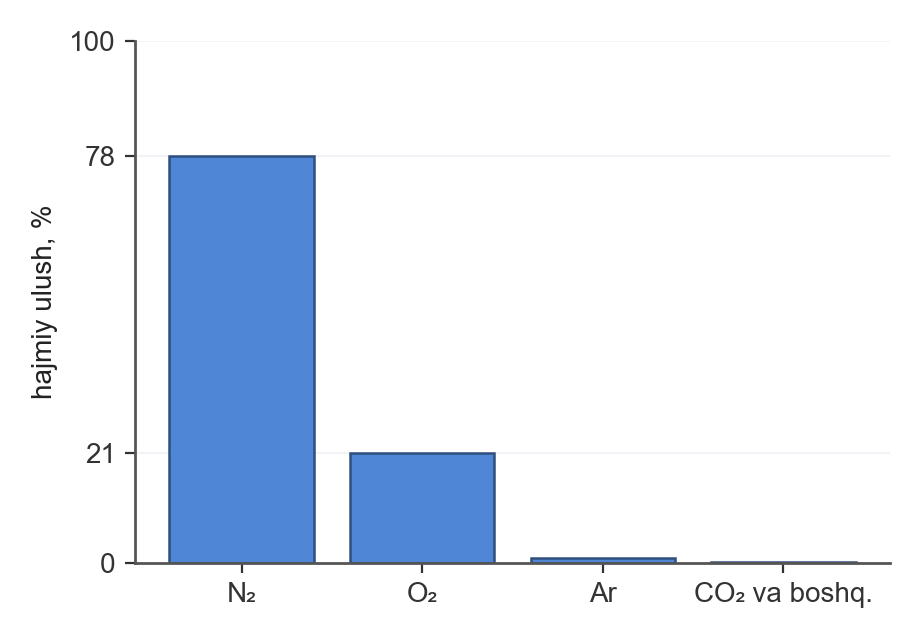
\includegraphics[width=0.86\linewidth]{rasmlar/gen/ai_v01_0.png}\end{center}
100 l (n.sh.) havo tarkibidagi kislorod \textbf{hajmini (l) toping.}

\noindent A)~\textsl{78} \hfill B)~\textsl{42} \hfill C)~\textsl{10,5} \hfill D)~\textsl{21}\par
\qsep
\noindent\qn{5.} CO + H\textsubscript{2}O $\rightleftarrows$ CO\textsubscript{2} + H\textsubscript{2} reaksiyasi 1 l hajmli idishda o`tkazildi. Ma'lumotlar jadvalda berilgan:
\begin{center}
\renewcommand{\arraystretch}{1.15}
\fitbox{\begin{tabular}{|c|c|c|c|}\hline
\textbf{Modda} & \textbf{CO} & \textbf{H\textsubscript{2}O} & \textbf{CO\textsubscript{2}} \\ \hline
Boshlang`ich, mol & 4 & 3 & 0 \\ \hline
Muvozanatda, mol & --- & --- & 1,5 \\ \hline
\end{tabular}}
\end{center}
Muvozanat \textbf{konstantasini (K) hisoblang.}

\noindent A)~\textsl{1,2} \hfill B)~\textsl{0,3} \hfill C)~\textsl{1,667} \hfill D)~\textsl{0,6}\par
\qsep
\noindent\qn{6.} 1 M sirka kislota eritmasida dissotsilanish darajasi 1\% bo`lsa, vodorod ionlari \textbf{konsentratsiyasini (mol/l) aniqlang.}

\noindent A)~\textsl{0,1} \hfill B)~\textsl{0,001} \hfill C)~\textsl{0,01} \hfill D)~\textsl{1}\par
\qsep
\noindent\qn{7.} 1,5 mol CH\textsubscript{4} tarkibida necha mol atom bor?

\noindent A)~\textsl{7,5} \hfill B)~\textsl{6} \hfill C)~\textsl{9} \hfill D)~\textsl{1,5}\par
\qsep
\noindent\qn{8.} 2SO\textsubscript{2} + O\textsubscript{2} $\rightleftarrows$ 2SO\textsubscript{3} + Q muvozanatni o`ngga siljitadigan \textbf{o`zgarishlarni toping}: 1) haroratni oshirish; 2) bosimni oshirish; 3) bosimni pasaytirish; 4) katalizator qo`shish.

\noindent A)~\textsl{2} \hfill B)~\textsl{3, 4} \hfill C)~\textsl{2, 4} \hfill D)~\textsl{2, 3}\par
\qsep
\noindent\qn{9.} Noma'lum \textit{X} tuzining eruvchanligi (g/100 g suv) haroratga bog`liq jadvalda keltirilgan:
\begin{center}
\renewcommand{\arraystretch}{1.15}
\fitbox{\begin{tabular}{|c|c|c|c|c|}\hline
\textbf{t, \textdegree{}C} & \textbf{0} & \textbf{20} & \textbf{40} & \textbf{60} \\ \hline
S, g/100 g suv & 13 & 32 & 64 & 110 \\ \hline
\end{tabular}}
\end{center}
40 \textdegree{}C da tayyorlangan to`yingan 164 g eritma 0 \textdegree{}C gacha sovitildi. Cho`kmaga tushgan tuz \textbf{massasini (g) aniqlang.}

\noindent A)~\textsl{64} \hfill B)~\textsl{51} \hfill C)~\textsl{13} \hfill D)~\textsl{102}\par
\qsep
\noindent\qn{10.} Quyidagi moddalarning qaysilarida ion bog` mavjud? 1) CO\textsubscript{2}; 2) NaOH; 3) Cl\textsubscript{2}; 4) KNO\textsubscript{3}

\noindent A)~\textsl{2, 3} \hfill B)~\textsl{1, 2, 3} \hfill C)~\textsl{2, 4} \hfill D)~\textsl{2, 3, 4}\par
\qsep
\noindent\qn{11.} Selen (\textit{Z} = 34) atomining tashqi energetik pog`onasidagi elektronlar \textbf{sonini aniqlang.}

\noindent A)~\textsl{7} \hfill B)~\textsl{6} \hfill C)~\textsl{5} \hfill D)~\textsl{8}\par
\qsep
\noindent\qn{12.} Quyidagi zarrachalardan qaysilari neon atomi bilan izoelektron? 1) Al\textsuperscript{3+}; 2) O\textsuperscript{2$-$}; 3) F\textsuperscript{$-$}; 4) Cl\textsuperscript{$-$}

\noindent A)~\textsl{1, 3} \hfill B)~\textsl{1, 2, 3} \hfill C)~\textsl{1, 2} \hfill D)~\textsl{2, 4}\par
\qsep
\noindent\qn{13.} NaCrO\textsubscript{2} + Br\textsubscript{2} + NaOH $\to$ Na\textsubscript{2}CrO\textsubscript{4} + NaBr + H\textsubscript{2}O reaksiya tenglamasini tenglang va barcha koeffitsiyentlar \textbf{yig`indisini aniqlang.}

\noindent A)~\textsl{26} \hfill B)~\textsl{25} \hfill C)~\textsl{24} \hfill D)~\textsl{27}\par
\qsep
\noindent\qn{14.} Reaksiya tenglamasi: 2CO + O\textsubscript{2} $\to$ 2CO\textsubscript{2}. Reaksiyaga 5,6 g CO kirishdi. CO\textsubscript{2} \textbf{hajmini (l, n.sh.) hisoblang.}

\noindent A)~\textsl{8,96} \hfill B)~\textsl{2,24} \hfill C)~\textsl{4,48} \hfill D)~\textsl{6,72}\par
\qsep
\noindent\qn{15.} NaI va NaCl dan iborat 40 g aralashma orqali mo`l xlor o`tkazilganda aralashma massasi 18,3 g ga kamaydi. Aralashmadagi NaI ning massa \textbf{ulushini (\%) aniqlang.}

\noindent A)~\textsl{25} \hfill B)~\textsl{30} \hfill C)~\textsl{75} \hfill D)~\textsl{45,8}\par
\qsep
\noindent\qn{16.} 2Na\textsubscript{2}O\textsubscript{2} + 2CO\textsubscript{2} $\to$ 2Na\textsubscript{2}CO\textsubscript{3} + O\textsubscript{2} jarayoni uchun 5,6 l (n.sh.) CO\textsubscript{2} olingan. Na\textsubscript{2}CO\textsubscript{3} \textbf{miqdorini (mol) aniqlang.}

\noindent A)~\textsl{0,5} \hfill B)~\textsl{0,12} \hfill C)~\textsl{0,38} \hfill D)~\textsl{0,25}\par
\qsep
\noindent\qn{17.} Rasmda metallarning kuchlanish qatori ko`rsatilgan (\textit{X}, \textit{Y}, \textit{Z} --- noma'lum metallar).
\begin{center}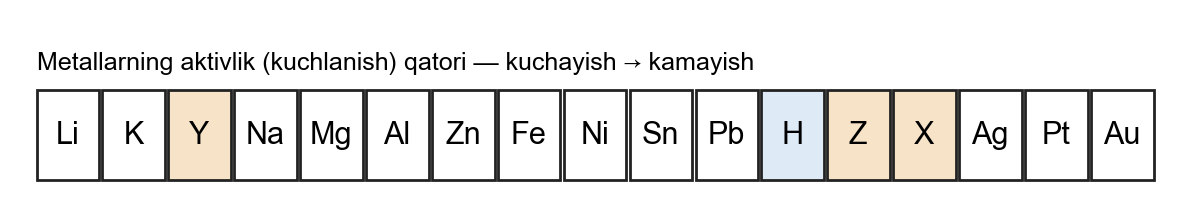
\includegraphics[width=0.86\linewidth]{rasmlar/gen/se_968458.png}\end{center}
\textit{Z} metali tuzining eritmasiga \textit{X} metall plastinka tushirilsa, reaksiya boradimi?
\noindent A)~\textsl{Boradi, \textit{X} faolroq}\par
\noindent B)~\textsl{Faqat qizdirilganda boradi}\par
\noindent C)~\textsl{Faqat konsentrlangan eritmada boradi}\par
\noindent D)~\textsl{Bormaydi, \textit{X} kamroq faol}\par
\qsep
\noindent\qn{18.} D-metallar va ularning birikmalari haqida qaysi fikrlar to`g`ri? 1) Temir sovuq konsentrlangan HNO\textsubscript{3} da passivlanadi; 2) Rux eritmada Fe\textsuperscript{2+} ni siqib chiqara olmaydi; 3) Xrom (VI) oksidi (CrO\textsubscript{3}) kislotali oksid; 4) Fe(OH)\textsubscript{2} havoda qo`ng`ir rangga o`tadi

\noindent A)~\textsl{2, 3, 4} \hfill B)~\textsl{1, 3, 4} \hfill C)~\textsl{1, 2} \hfill D)~\textsl{1, 3}\par
\qsep
\noindent\qn{19.} 1 l suvda 0,01 mol Ca(HCO\textsubscript{3})\textsubscript{2}, 0,01 mol CaSO\textsubscript{4} va 0,03 mol MgCl\textsubscript{2} erigan. Suv qaynatilgandan keyin qolgan qattiqlikni yo`qotish uchun necha gramm soda (Na\textsubscript{2}CO\textsubscript{3}) kerak?

\noindent A)~\textsl{5,3} \hfill B)~\textsl{1,06} \hfill C)~\textsl{3,18} \hfill D)~\textsl{4,24}\par
\qsep
\noindent\qn{20.} CH\textsubscript{3}--C(CH\textsubscript{3})\textsubscript{2}--OH birikmaning sistematik nomi qaysi qatorda to`g`ri keltirilgan?

\noindent\begin{tabular}{@{}p{0.47\linewidth}@{}p{0.47\linewidth}@{}}
A)~\textsl{2-metilpropanol-2} & B)~\textsl{butanol-2} \\
C)~\textsl{2-metilpropanol-1} & D)~\textsl{butanol-1} \\
\end{tabular}\par
\qsep
\noindent\qn{21.} 46 g etil spirtidan Lebedev usuli bilan (90\% unum) butadiyen-1,3 olindi (2C\textsubscript{2}H\textsubscript{5}OH $\to$ C\textsubscript{4}H\textsubscript{6} + H\textsubscript{2} + 2H\textsubscript{2}O). Butadiyen \textbf{massasini (g) aniqlang.}

\noindent A)~\textsl{48,6} \hfill B)~\textsl{27} \hfill C)~\textsl{46} \hfill D)~\textsl{24,3}\par
\qsep
\noindent\qn{22.} Arenlar, neft va tabiiy gaz haqida qaysi fikrlar to`g`ri? 1) Benzolda 6 ta sp\textsuperscript{2} gibridlangan uglerod bor; 2) Neft fraksiyalaridan gazolin 150 \textdegree{}C gacha haydaladi; 3) Naftalin -- bir halqali aren; 4) Benzol bromli suvni rangsizlantirmaydi

\noindent A)~\textsl{1, 3, 4} \hfill B)~\textsl{1, 4} \hfill C)~\textsl{2, 4} \hfill D)~\textsl{1, 2, 4}\par
\qsep
\noindent\qn{23.} 2C\textsubscript{2}H\textsubscript{5}OH + 2Na $\to$ 2C\textsubscript{2}H\textsubscript{5}ONa + H\textsubscript{2} reaksiyasida 4,6 g Na ishtirok etdi (unum 90\%). C\textsubscript{2}H\textsubscript{5}ONa \textbf{massasini (g) toping.}

\noindent A)~\textsl{13,6} \hfill B)~\textsl{12,24} \hfill C)~\textsl{24,48} \hfill D)~\textsl{6,12}\par
\qsep
\noindent\qn{24.} 2CH\textsubscript{3}CHO + 5O\textsubscript{2} $\to$ 4CO\textsubscript{2} + 4H\textsubscript{2}O jarayoni uchun 88 g CH\textsubscript{3}CHO olingan. CO\textsubscript{2} \textbf{massasini (g) aniqlang.}

\noindent A)~\textsl{44} \hfill B)~\textsl{176} \hfill C)~\textsl{352} \hfill D)~\textsl{88}\par
\qsep
\noindent\qn{25.} Karbon kislotalar haqida qaysi fikrlar to`g`ri? 1) Benzoy kislota Na\textsubscript{2}CO\textsubscript{3} bilan reaksiyaga kirishmaydi; 2) Sirka kislota karbonatlar bilan CO\textsubscript{2} ajratadi; 3) Karboksil guruh karbonil va gidroksil guruhlardan iborat; 4) Stearin kislota to`yinmagan kislota

\noindent A)~\textsl{2, 3} \hfill B)~\textsl{1, 4} \hfill C)~\textsl{1, 3, 4} \hfill D)~\textsl{2, 3, 4}\par
\qsep
\noindent\qn{26.} 17,6 g CH\textsubscript{3}COOC\textsubscript{2}H\textsubscript{5} mo`l NaOH bilan to`liq gidrolizlandi. Hosil bo`lgan spirt \textbf{massasini (g) aniqlang.}

\noindent A)~\textsl{17,6} \hfill B)~\textsl{18,4} \hfill C)~\textsl{9,2} \hfill D)~\textsl{16,4}\par
\qsep
\noindent\qn{27.} Uglevodlar haqida qaysi fikrlar to`g`ri? 1) Fruktoza ketospirt; 2) Glyukoza gidrolizlanadi; 3) Saxaroza Feling suyuqligini qaytaradi; 4) Kraxmal yod bilan ko`k rang beradi

\noindent A)~\textsl{1, 4} \hfill B)~\textsl{1, 2} \hfill C)~\textsl{2, 4} \hfill D)~\textsl{2}\par
\qsep
\noindent\qn{28.} 18,6 g anilin mo`l xlorid kislota bilan reaksiyaga kirishganda hosil bo`lgan tuz \textbf{massasini (g) aniqlang.}

\noindent A)~\textsl{18,6} \hfill B)~\textsl{51,8} \hfill C)~\textsl{25,9} \hfill D)~\textsl{7,3}\par
\qsep
\noindent\qn{29.} C\textsubscript{2}H\textsubscript{5}Cl + KOH (spirt) reaksiyasi natijasida qaysi organik modda hosil bo`ladi?

\noindent\begin{tabular}{@{}p{0.47\linewidth}@{}p{0.47\linewidth}@{}}
A)~\textsl{etilatsetat} & B)~\textsl{etilen} \\
C)~\textsl{etanol} & D)~\textsl{anilin} \\
\end{tabular}\par
\qsep
\noindent\qn{30.} Rasmda HCl ning suvda erishi ko`rsatilgan. 22,4 l (n.sh.) HCl 1000 g suvda eritilsa, hosil bo`lgan eritmadagi HCl ning massa ulushi necha foiz?
\begin{center}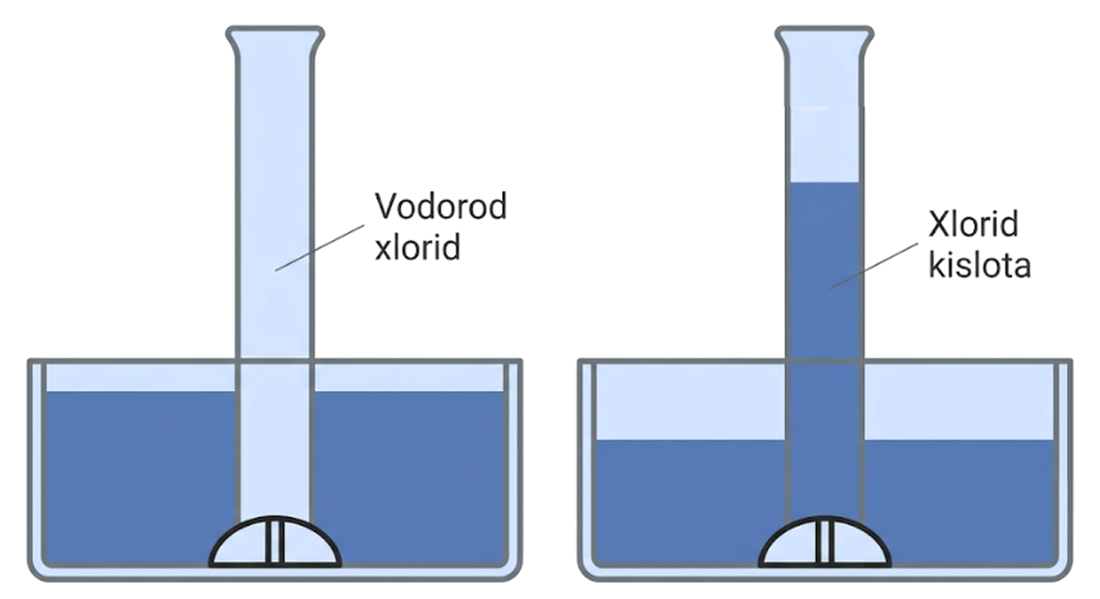
\includegraphics[width=0.86\linewidth]{rasmlar/darslik/d_hcl_erish.png}\end{center}

\noindent A)~\textsl{3,52} \hfill B)~\textsl{3,65} \hfill C)~\textsl{1,76} \hfill D)~\textsl{7,04}\par
\qsep
\noindent\qn{31.} Fenolftalein indikatori ishqoriy muhitda qanday rang beradi?
\noindent A)~\textsl{malina rangga kiradi (pushti)}\par
\noindent B)~\textsl{sariq}\par
\noindent C)~\textsl{binafsha}\par
\noindent D)~\textsl{rangsiz}\par
\qsep
\noindent\qn{32.} Laboratoriyada asetilen olish uchun qaysi moddalar ishlatiladi?
\noindent A)~\textsl{KMnO\textsubscript{4} (qizdirish)}\par
\noindent B)~\textsl{C\textsubscript{2}H\textsubscript{5}OH + H\textsubscript{2}SO\textsubscript{4} (kons.), 170 \textdegree{}C}\par
\noindent C)~\textsl{CaCO\textsubscript{3} + HCl}\par
\noindent D)~\textsl{CaC\textsubscript{2} + H\textsubscript{2}O   ---}\par
\qsep
\end{multicols}
\medskip
\noindent\setlength{\fboxsep}{0pt}\fbox{\begin{tabular}{p{0.74\linewidth}|p{0.2\linewidth}}
\parbox[t]{0.72\linewidth}{\vspace{3pt}\textbf{Topshiriqlar (33--35) va javob variant (A--F)larini o`zaro to`g`ri moslashtiring.} CaC\textsubscript{2} (12,8 g) va Al\textsubscript{4}C\textsubscript{3} (7,2 g) dan iborat aralashma mo`l suv bilan to`liq reaksiyaga kirishdi.
\vspace{3pt}} & \parbox[t]{0.19\linewidth}{\vspace{3pt}A~\textsl{7,04}\\[3pt]
B~\textsl{85,33}\\[3pt]
C~\textsl{5,43}\\[3pt]
D~\textsl{5,63}\\[3pt]
E~\textsl{10,86}\\[3pt]
F~\textsl{42,67}}\\ \hline
\parbox[t]{0.72\linewidth}{\vspace{2pt}\textbf{33. Hosil bo`lgan gazlar aralashmasining vodorodga nisbatan zichligini aniqlang.}\vspace{2pt}} & \\ \hline
\parbox[t]{0.72\linewidth}{\vspace{2pt}\textbf{34. Hosil bo`lgan gazlar aralashmasini to`liq yoqish uchun zarur havo hajmini (l, n.sh.; havoda 21\% kislorod bor) aniqlang.}\vspace{2pt}} & \\ \hline
\parbox[t]{0.72\linewidth}{\vspace{2pt}\textbf{35. Aralashmadagi to`yinmagan uglevodorod Kucherov reaksiyasi bo`yicha 80\% unum bilan reaksiyaga kirishsa, hosil bo`lgan aldegid massasini (g) aniqlang.}\vspace{2pt}} & 
\end{tabular}}
\par\bigskip
\noindent\qn{36.} Fe + H\textsubscript{2}SO\textsubscript{4} $\to$ Fe\textsubscript{2}(SO\textsubscript{4})\textsubscript{3} + SO\textsubscript{2} + H\textsubscript{2}O reaksiya tenglamasini tenglang va barcha koeffitsiyentlar \textbf{yig`indisini aniqlang.}
\javob\qsep
\noindent\qn{37.} pH = 1 bo`lgan kuchli kislota eritmasi 100 marta suyultirildi. Yangi eritmaning pH \textbf{qiymatini aniqlang.}
\javob\qsep
\noindent\qn{38.} Cu va CuO dan iborat 16,8 g aralashma mo`l suyultirilgan H\textsubscript{2}SO\textsubscript{4} da ishlandi, 12,8 g qattiq qoldiq qoldi. Hosil bo`lgan tuz \textbf{massasini (g) aniqlang.}
\javob\qsep
\noindent\qn{39.} C\textsubscript{3}H\textsubscript{7}OH va C\textsubscript{2}H\textsubscript{5}OH dan iborat 10,6 g aralashma natriy bilan to`liq reaksiyaga kirishganda 2,24 l (n.sh.) vodorod ajraldi. Aralashmadagi C\textsubscript{3}H\textsubscript{7}OH \textbf{massasini (g) toping.}
\javob\qsep
\noindent\qn{40.} 17,8 g tristearin mo`l NaOH eritmasi bilan to`liq gidrolizlandi (sovun unumi 80\%). Hosil bo`lgan natriy stearat (M = 306 g/mol) \textbf{massasini (g) toping.}
\javob\qsep
\par\bigskip\begin{center}\textbf{\fontsize{13}{15}\selectfont YOZMA ISH}\end{center}
\noindent\qn{41.} \textbf{Topshiriqni bajarish jarayonida barcha reaksiya tenglamalarini yozing. Miqdoriy va arifmetik hisoblashlarni (unga asos bo`lgan usul yoki formulani ko`rsatgan holda) uzviy ketma-ketlikda bajaring.}\par\smallskip
Sulfat kislotaning massa ulushi 40\% bo`lgan eritmasining zichligi 1,3 g/ml.\par
\noindent 1)\ Eritmaning molyar konsentratsiyasini (mol/l) hisoblang.\par
\noindent 2)\ Eritmaning normal konsentratsiyasini (ekv/l) toping. Sulfat kislotaning ekvivalent massasini (g/ekv) ham aniqlang.\par
\noindent 3)\ Eritmaning molyal konsentratsiyasini (mol/kg) aniqlang.\par
\noindent 4)\ Shu eritmadan 100 ml 0,5 mol/l li eritma tayyorlash uchun necha ml olish kerak? 100 ml eritmadagi suvning massasini (g) ham hisoblang.\par
\noindent 5)\ 100 ml shu eritmani to`liq neytrallash uchun necha gramm NaOH kerak? 250 ml shu eritmadagi H\textsubscript{2}SO\textsubscript{4} massasini (g) ham hisoblang.\par
\diqqat{Mazkur topshiriq kengaytirilgan javobni talab etib, uning yechilish usuli va shu usul asosidagi barcha hisoblash amallari javoblar varaqasida aks etishi lozim.}\qsep
\noindent\qn{42.} Quyidagi o`zgarishlar zanjirida \textit{X}, \textit{Y}, \textit{Z} noma'lum organik moddalar:\par
\[\setlength{\fboxsep}{0pt}\text{CH\textsubscript{3}CHO}\xrightarrow{\text{Ag\textsubscript{2}O, NH\textsubscript{3}}}\text{\textit{X}}\xrightarrow{\text{C\textsubscript{2}H\textsubscript{5}OH, H\textsubscript{2}SO\textsubscript{4}}}\text{\textit{Y}}\xrightarrow{\text{NaOH}}\text{\textit{Z}}\xrightarrow{\text{NaOH (suyuqlanma), t\textdegree{}}}\text{CH\textsubscript{4}}\]
\noindent 1)\ CH\textsubscript{3}CHO $\to$ \textit{X} : reaksiya tenglamasini yozing; hosil bo`lgan moddani nomlang.\par
\noindent 2)\ \textit{X} $\to$ \textit{Y} : reaksiya tenglamasini yozing; hosil bo`lgan moddani nomlang.\par
\noindent 3)\ \textit{Y} $\to$ \textit{Z} : reaksiya tenglamasini yozing; hosil bo`lgan moddani nomlang.\par
\noindent 4)\ \textit{Z} $\to$ CH\textsubscript{4} : reaksiya tenglamasini yozing; hosil bo`lgan moddani nomlang.\par
\diqqat{Mazkur topshiriq kengaytirilgan javobni talab etib, uning yechilish usuli va shu usul asosidagi barcha hisoblash amallari javoblar varaqasida aks etishi lozim.}\qsep
\noindent\qn{43.} \textbf{Topshiriqni bajarish jarayonida barcha reaksiya tenglamalarini yozing. Miqdoriy va arifmetik hisoblashlarni (unga asos bo`lgan usul yoki formulani ko`rsatgan holda) uzviy ketma-ketlikda bajaring.}\par\smallskip
SO\textsubscript{2} va CO\textsubscript{2} dan iborat 6,72 l (n.sh.) gazlar aralashmasi avval mo`l bromli suvdan, so`ngra mo`l Ba(OH)\textsubscript{2} eritmasidan o`tkazildi. Bromli suvdan o`tgandan keyin SO\textsubscript{2} to`liq yutildi.\par
\noindent 1)\ Bromli suv bilan SO\textsubscript{2} reaksiyasi tenglamasini yozing (SO\textsubscript{2} + Br\textsubscript{2} + 2H\textsubscript{2}O $\to$ H\textsubscript{2}SO\textsubscript{4} + 2HBr). Hosil bo`lgan H\textsubscript{2}SO\textsubscript{4} massasini (g) toping. SO\textsubscript{2} hajmini (l, n.sh.) ham hisoblang.\par
\noindent 2)\ Mo`l BaCl\textsubscript{2} qo`shilganda bromli suvli eritmada hosil bo`lgan cho`kma massasini (g) aniqlang.\par
\noindent 3)\ Ba(OH)\textsubscript{2} eritmasida hosil bo`lgan cho`kma massasini (g) hisoblang.\par
\noindent 4)\ Dastlabki aralashmaning o`rtacha molyar massasini (g/mol) va havoga nisbatan zichligini toping.\par
\noindent 5)\ Bromli suvli eritmada hosil bo`lgan HBr massasini (g) hisoblang.\par
\diqqat{Mazkur topshiriq kengaytirilgan javobni talab etib, uning yechilish usuli va shu usul asosidagi barcha hisoblash amallari javoblar varaqasida aks etishi lozim.}\qsep
\newpage
\renewcommand{\curvar}{2-variant}
\thispagestyle{first}
\noindent\textit{Davriy jadvaldan foydalanish mumkin.}
\par\smallskip
\begin{multicols}{2}
\noindent\qn{1.} Jadvalda ikki tuz eritmasi haqida ma'lumot berilgan:
\begin{center}
\renewcommand{\arraystretch}{1.15}
\fitbox{\begin{tabular}{|c|c|c|}\hline
\textbf{Eritma} & \textbf{Massasi, g} & \textbf{Massa ulushi, \%} \\ \hline
1 & 100 & 20 \\ \hline
2 & 200 & 30 \\ \hline
\end{tabular}}
\end{center}
Eritmalar aralashtirilganda hosil bo`lgan eritmaning massa \textbf{ulushini (\%) aniqlang.}

\noindent A)~\textsl{26,67} \hfill B)~\textsl{25} \hfill C)~\textsl{50} \hfill D)~\textsl{23,33}\par
\qsep
\noindent\qn{2.} CuSO\textsubscript{4}$\cdot$5H\textsubscript{2}O kristallogidratida kristallizatsion suvning massa \textbf{ulushini (\%) aniqlang.}

\noindent A)~\textsl{64} \hfill B)~\textsl{36} \hfill C)~\textsl{18} \hfill D)~\textsl{56,2}\par
\qsep
\noindent\qn{3.} 2-davr elementlari atom radiuslarining o`zgarishi diagrammada ko`rsatilgan.
\begin{center}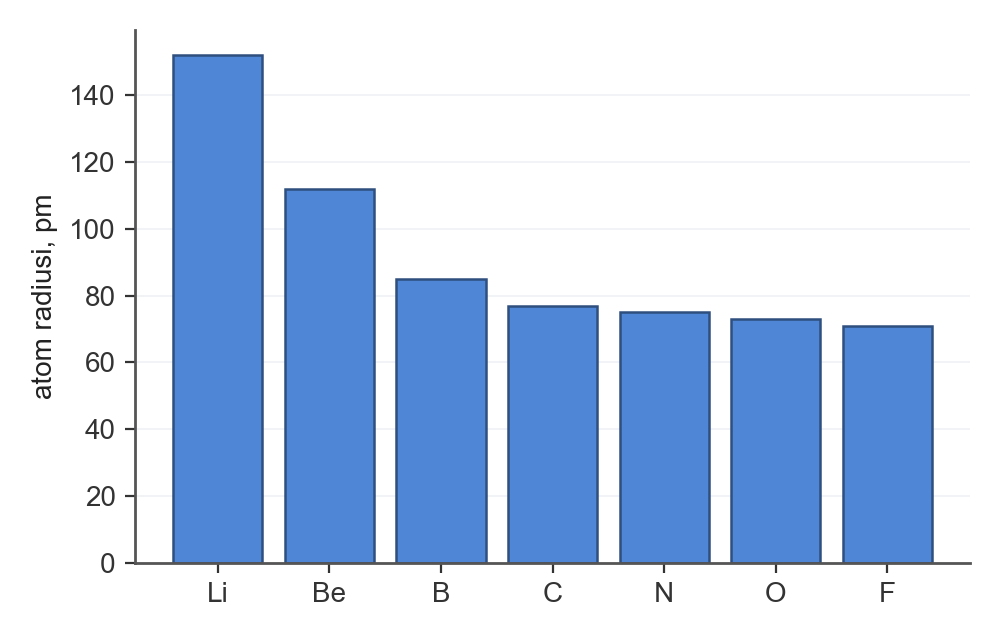
\includegraphics[width=0.86\linewidth]{rasmlar/gen/ra_v02_0.png}\end{center}
Davr bo`yicha chapdan o`ngga atom radiusi qanday o`zgaradi va sababi nima?
\noindent A)~\textsl{Ortadi, qavatlar soni ko`payishi tufayli}\par
\noindent B)~\textsl{Kamayadi, qavatlar soni kamayishi tufayli}\par
\noindent C)~\textsl{O`zgarmaydi}\par
\noindent D)~\textsl{Kamayadi, yadro zaryadi ortishi tufayli}\par
\qsep
\noindent\qn{4.} Rasmda radioaktiv yemirilish zanjiri berilgan (massa soni/zaryad; ``?'' -- oraliq yadrolar).
\begin{center}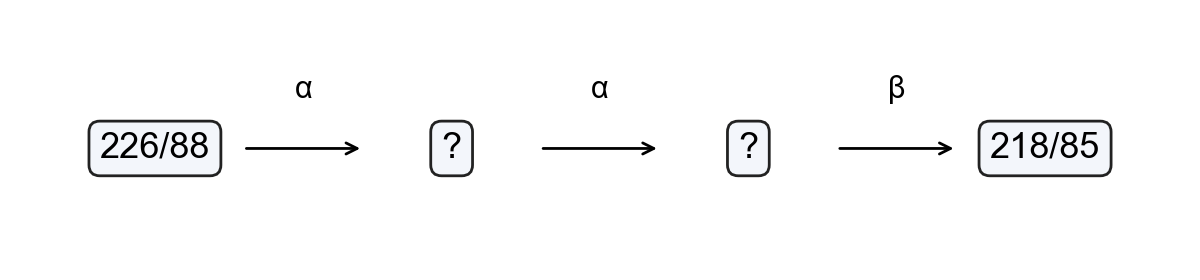
\includegraphics[width=0.86\linewidth]{rasmlar/gen/dc_297842.png}\end{center}
Oxirgi yadroning massa \textbf{sonini aniqlang.}

\noindent A)~\textsl{222} \hfill B)~\textsl{214} \hfill C)~\textsl{219} \hfill D)~\textsl{218}\par
\qsep
\noindent\qn{5.} Tarkibida 30\% SO\textsubscript{3} bo`lgan 100 g oleum 300 g suvga qo`shildi. Hosil bo`lgan eritmadagi H\textsubscript{2}SO\textsubscript{4} ning massa \textbf{ulushini (\%) aniqlang.}

\noindent A)~\textsl{17,5} \hfill B)~\textsl{26,69} \hfill C)~\textsl{35,58} \hfill D)~\textsl{40,03}\par
\qsep
\noindent\qn{6.} N\textsubscript{2} + 3H\textsubscript{2} $\rightleftarrows$ 2NH\textsubscript{3} reaksiyada muvozanat holatida [N\textsubscript{2}] = 1, [H\textsubscript{2}] = 0,5, [NH\textsubscript{3}] = 2 mol/l. Muvozanat \textbf{konstantasini (K) hisoblang.}

\noindent A)~\textsl{64} \hfill B)~\textsl{16} \hfill C)~\textsl{32} \hfill D)~\textsl{4}\par
\qsep
\noindent\qn{7.} 3 mol Al\textsubscript{2}(SO\textsubscript{4})\textsubscript{3} va 3 mol AlCl\textsubscript{3} suvda eritilib, eritma hajmi 2 l ga yetkazildi. Eritmadagi barcha ionlarning umumiy molyar \textbf{konsentratsiyasini (mol/l) aniqlang} (kuchli elektrolitlar to`liq dissotsilanadi).

\noindent A)~\textsl{3} \hfill B)~\textsl{27} \hfill C)~\textsl{13,5} \hfill D)~\textsl{6,75}\par
\qsep
\noindent\qn{8.} Jadvalda metall plastinkalarning tuz eritmalariga tushirilishidagi kuzatuvlar berilgan (``+'' -- metall ajraladi, reaksiya boradi; ``$-$'' -- reaksiya bormaydi):
\begin{center}
\renewcommand{\arraystretch}{1.15}
\fitbox{\begin{tabular}{|c|c|c|c|}\hline
\textbf{Metall} & \textbf{ZnSO\textsubscript{4} eritmasi} & \textbf{AgNO\textsubscript{3} eritmasi} & \textbf{CuSO\textsubscript{4} eritmasi} \\ \hline
Mg & + & + & + \\ \hline
Cu & $-$ & + & $-$ \\ \hline
Zn & $-$ & + & + \\ \hline
\end{tabular}}
\end{center}
Ushbu metallardan qaysi biri eng faol?

\noindent A)~\textsl{Cu} \hfill B)~\textsl{Mg} \hfill C)~\textsl{Zn} \hfill D)~\textsl{Fe}\par
\qsep
\noindent\qn{9.} 10 l H\textsubscript{2}S va 45 l O\textsubscript{2} aralashmasi 2H\textsubscript{2}S + 3O\textsubscript{2} $\to$ 2SO\textsubscript{2} + 2H\textsubscript{2}O tenglama bo`yicha to`liq reaksiyaga kirishdi (reaksiyadan so`ng suv suyuq holatda; gazlar bir xil sharoitda o`lchandi). Aralashma hajmi necha litrga o`zgargan (modul bo`yicha)?

\noindent A)~\textsl{55} \hfill B)~\textsl{40} \hfill C)~\textsl{10} \hfill D)~\textsl{15}\par
\qsep
\noindent\qn{10.} 8 g metall kislotada eritilganda 4,48 l (n.sh.) vodorod ajraldi. Metallning ekvivalent \textbf{massasini (g/mol) aniqlang} (\textit{V}\_E(H\textsubscript{2}) = 11,2 l/mol).

\noindent A)~\textsl{40} \hfill B)~\textsl{10} \hfill C)~\textsl{89,6} \hfill D)~\textsl{20}\par
\qsep
\noindent\qn{11.} Azot (\textit{Z} = 7) atomida nechta juftlashmagan elektron bor?

\noindent A)~\textsl{4} \hfill B)~\textsl{2} \hfill C)~\textsl{5} \hfill D)~\textsl{3}\par
\qsep
\noindent\qn{12.} Zichligi 1,4 g/ml bo`lgan 40\% li KOH eritmasining molyar \textbf{konsentratsiyasini (mol/l) aniqlang.}

\noindent A)~\textsl{1} \hfill B)~\textsl{20} \hfill C)~\textsl{10} \hfill D)~\textsl{7,14}\par
\qsep
\noindent\qn{13.} 61,25 g KClO\textsubscript{3} reaksiyaga kirishdi (2KClO\textsubscript{3} $\to$ 2KCl + 3O\textsubscript{2}). Ajralgan O\textsubscript{2} \textbf{hajmini (l, n.sh.) hisoblang} (unum 80\%).

\noindent A)~\textsl{13,44} \hfill B)~\textsl{16,8} \hfill C)~\textsl{26,88} \hfill D)~\textsl{6,72}\par
\qsep
\noindent\qn{14.} Ishqoriy metallar haqida qaysi fikrlar to`g`ri? 1) Ishqoriy metallar tabiatda erkin holda uchraydi; 2) Natriy yonganda Na\textsubscript{2}O\textsubscript{2} hosil bo`ladi; 3) Natriy kerosin ostida saqlanadi; 4) Litiy eng yengil metall

\noindent A)~\textsl{1, 2, 3} \hfill B)~\textsl{1, 4} \hfill C)~\textsl{2, 3, 4} \hfill D)~\textsl{1, 3}\par
\qsep
\noindent\qn{15.} Ca + 2H\textsubscript{2}O $\to$ Ca(OH)\textsubscript{2} + H\textsubscript{2} reaksiyasida 20 g Ca ishtirok etdi. H\textsubscript{2} \textbf{massasini (g) toping.}

\noindent A)~\textsl{1} \hfill B)~\textsl{2} \hfill C)~\textsl{0,5} \hfill D)~\textsl{1,5}\par
\qsep
\noindent\qn{16.} 11,2 g temir bir qismi xlor bilan, xuddi shuncha qismi xlorid kislota bilan reaksiyaga kirishdi. Hosil bo`lgan tuzlar massalari \textbf{farqini (g) aniqlang.}

\noindent A)~\textsl{32,5} \hfill B)~\textsl{25,4} \hfill C)~\textsl{14,2} \hfill D)~\textsl{7,1}\par
\qsep
\noindent\qn{17.} Reaksiya tenglamasi: Mg(HCO\textsubscript{3})\textsubscript{2} $\to$ MgCO\textsubscript{3} + CO\textsubscript{2} + H\textsubscript{2}O. Reaksiyaga 58,4 g Mg(HCO\textsubscript{3})\textsubscript{2} kirishdi (unum 50\%). CO\textsubscript{2} \textbf{miqdorini (mol) hisoblang.}

\noindent A)~\textsl{0,2} \hfill B)~\textsl{0,4} \hfill C)~\textsl{0,1} \hfill D)~\textsl{0,3}\par
\qsep
\noindent\qn{18.} Qaysi juftliklar o`zaro reaksiyaga kirishmaydi? 1) Fe\textsubscript{2}O\textsubscript{3} va H\textsubscript{2}O; 2) SiO\textsubscript{2} va H\textsubscript{2}O; 3) CO\textsubscript{2} va CaO; 4) ZnO va HCl

\noindent A)~\textsl{4} \hfill B)~\textsl{1, 2} \hfill C)~\textsl{1} \hfill D)~\textsl{2, 3, 4}\par
\qsep
\noindent\qn{19.} Reaksiya tenglamasi: 2Al + 3CuCl\textsubscript{2} $\to$ 2AlCl\textsubscript{3} + 3Cu. Reaksiyaga 27 g CuCl\textsubscript{2} kirishdi. Al \textbf{massasini (g) hisoblang.}

\noindent A)~\textsl{8,1} \hfill B)~\textsl{3,6} \hfill C)~\textsl{7,2} \hfill D)~\textsl{1,8}\par
\qsep
\noindent\qn{20.} C\textsubscript{4}H\textsubscript{9}OH tarkibli spirtlarning izomerlari soni nechta?

\noindent A)~\textsl{5} \hfill B)~\textsl{4} \hfill C)~\textsl{3} \hfill D)~\textsl{6}\par
\qsep
\noindent\qn{21.} 23 g etil spirtidan 90\% unum bilan etilen olindi. Etilen \textbf{hajmini (l, n.sh.) aniqlang.}

\noindent A)~\textsl{10,08} \hfill B)~\textsl{11,2} \hfill C)~\textsl{20,16} \hfill D)~\textsl{20,7}\par
\qsep
\noindent\qn{22.} Arenlar, neft va tabiiy gaz haqida qaysi fikrlar to`g`ri? 1) Benzolda 6 ta sp\textsuperscript{2} gibridlangan uglerod bor; 2) Benzol uchun birikish reaksiyalari mutlaqo xos emas; 3) Benzoldan nitrobenzol nitrolash bilan olinadi; 4) Naftalin -- bir halqali aren

\noindent A)~\textsl{1, 3, 4} \hfill B)~\textsl{1, 3} \hfill C)~\textsl{1, 4} \hfill D)~\textsl{1}\par
\qsep
\noindent\qn{23.} Spirt va fenollar haqida qaysi fikrlar to`g`ri? 1) Fenol Cu(OH)\textsubscript{2} ni eritib ko`k kompleks hosil qiladi; 2) Etanol natriy bilan reaksiyaga kirishadi; 3) Etilenglikol zaharsiz; 4) Birlamchi spirt oksidlanganda aldegid hosil bo`ladi

\noindent A)~\textsl{1, 2, 3} \hfill B)~\textsl{1, 2, 4} \hfill C)~\textsl{2, 4} \hfill D)~\textsl{1, 4}\par
\qsep
\noindent\qn{24.} Reaksiya tenglamasi: HCHO + Ag\textsubscript{2}O $\to$ HCOOH + 2Ag. Reaksiyaga 2,24 l (n.sh.) HCHO kirishdi. Ag\textsubscript{2}O \textbf{massasini (g) hisoblang.}

\noindent A)~\textsl{46,4} \hfill B)~\textsl{23,2} \hfill C)~\textsl{11,6} \hfill D)~\textsl{34,8}\par
\qsep
\noindent\qn{25.} 60 g CH\textsubscript{3}COOH dan quyidagi ikki bosqichda CH\textsubscript{4} olinadi: 1) CH\textsubscript{3}COOH + NaOH $\to$ CH\textsubscript{3}COONa + H\textsubscript{2}O (unum 50\%); 2) CH\textsubscript{3}COONa + NaOH $\to$ CH\textsubscript{4} + Na\textsubscript{2}CO\textsubscript{3} (unum 75\%). Oxirgi mahsulot CH\textsubscript{4} ning \textbf{hajmini (l, n.sh.) toping.}

\noindent A)~\textsl{16,8} \hfill B)~\textsl{11,2} \hfill C)~\textsl{8,4} \hfill D)~\textsl{22,4}\par
\qsep
\noindent\qn{26.} 445 g tristearin natriy ishqori bilan to`liq gidrolizlanganda necha gramm sovun hosil bo`ladi?

\noindent A)~\textsl{153} \hfill B)~\textsl{306} \hfill C)~\textsl{459} \hfill D)~\textsl{445}\par
\qsep
\noindent\qn{27.} 22 g CO\textsubscript{2} dan quyidagi ikki bosqichda C\textsubscript{2}H\textsubscript{5}OH olinadi: 1) 6CO\textsubscript{2} + 6H\textsubscript{2}O $\to$ C\textsubscript{6}H\textsubscript{12}O\textsubscript{6} + 6O\textsubscript{2} (unum 60\%); 2) C\textsubscript{6}H\textsubscript{12}O\textsubscript{6} $\to$ 2C\textsubscript{2}H\textsubscript{5}OH + 2CO\textsubscript{2} (unum 90\%). Oxirgi mahsulot C\textsubscript{2}H\textsubscript{5}OH ning \textbf{massasini (g) toping.}

\noindent A)~\textsl{4,14} \hfill B)~\textsl{6,9} \hfill C)~\textsl{4,6} \hfill D)~\textsl{7,67}\par
\qsep
\noindent\qn{28.} 24,6 g C\textsubscript{6}H\textsubscript{5}NO\textsubscript{2} dan quyidagi ikki bosqichda C\textsubscript{6}H\textsubscript{5}NH\textsubscript{3}Cl olinadi: 1) C\textsubscript{6}H\textsubscript{5}NO\textsubscript{2} + 3H\textsubscript{2} $\to$ C\textsubscript{6}H\textsubscript{5}NH\textsubscript{2} + 2H\textsubscript{2}O (unum 80\%); 2) C\textsubscript{6}H\textsubscript{5}NH\textsubscript{2} + HCl $\to$ C\textsubscript{6}H\textsubscript{5}NH\textsubscript{3}Cl (unum 75\%). Oxirgi mahsulot C\textsubscript{6}H\textsubscript{5}NH\textsubscript{3}Cl ning \textbf{massasini (g) toping.}

\noindent A)~\textsl{15,54} \hfill B)~\textsl{19,42} \hfill C)~\textsl{20,72} \hfill D)~\textsl{25,9}\par
\qsep
\noindent\qn{29.} 3C\textsubscript{2}H\textsubscript{2} (C, t) reaksiyasi natijasida qaysi organik modda hosil bo`ladi?

\noindent\begin{tabular}{@{}p{0.47\linewidth}@{}p{0.47\linewidth}@{}}
A)~\textsl{benzoy kislota} & B)~\textsl{etilatsetat} \\
C)~\textsl{benzol} & D)~\textsl{sirka aldegid} \\
\end{tabular}\par
\qsep
\noindent\qn{30.} Uch probirkada (\textit{X}, \textit{Y}, \textit{Z}) Na\textsubscript{2}SO\textsubscript{4}, K\textsubscript{2}CO\textsubscript{3}, NH\textsubscript{4}Cl eritmalari bor (tartibsiz). Ularga HCl va NaOH ta'sir ettirildi. Kuzatuvlar jadvalda:
\begin{center}
\renewcommand{\arraystretch}{1.15}
\fitbox{\begin{tabular}{|c|c|c|}\hline
\textbf{Probirka} & \textbf{HCl qo`shilganda} & \textbf{NaOH qo`shib qizdirilganda} \\ \hline
\textit{X} & o`zgarish yo`q & o`tkir hidli gaz ajraladi \\ \hline
\textit{Y} & o`zgarish yo`q & o`zgarish yo`q \\ \hline
\textit{Z} & gaz ajraladi & o`zgarish yo`q \\ \hline
\end{tabular}}
\end{center}
\textit{X}, \textit{Y}, \textit{Z} probirkalardagi \textbf{moddalarni aniqlang.}
\noindent A)~\textsl{\textit{X} -- K\textsubscript{2}CO\textsubscript{3}, \textit{Y} -- NH\textsubscript{4}Cl, \textit{Z} -- Na\textsubscript{2}SO\textsubscript{4}}\par
\noindent B)~\textsl{\textit{X} -- NH\textsubscript{4}Cl, \textit{Y} -- K\textsubscript{2}CO\textsubscript{3}, \textit{Z} -- Na\textsubscript{2}SO\textsubscript{4}}\par
\noindent C)~\textsl{\textit{X} -- Na\textsubscript{2}SO\textsubscript{4}, \textit{Y} -- NH\textsubscript{4}Cl, \textit{Z} -- K\textsubscript{2}CO\textsubscript{3}}\par
\noindent D)~\textsl{\textit{X} -- NH\textsubscript{4}Cl, \textit{Y} -- Na\textsubscript{2}SO\textsubscript{4}, \textit{Z} -- K\textsubscript{2}CO\textsubscript{3}}\par
\qsep
\noindent\qn{31.} Rasmda spirt lampasining tuzilishi ko`rsatilgan. 1 raqami bilan \textbf{belgilang}an qism nima deb ataladi?
\begin{center}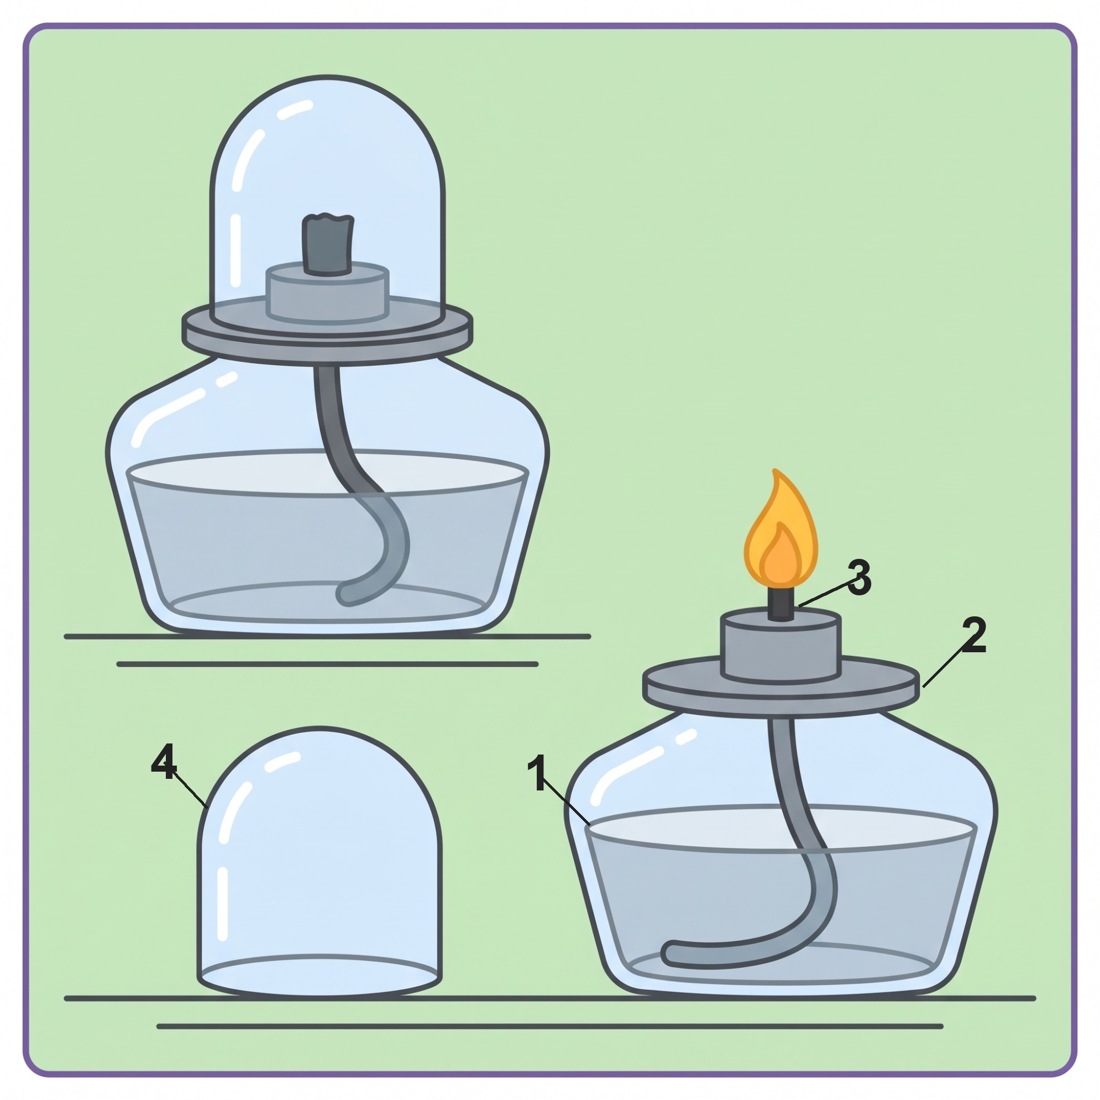
\includegraphics[width=0.86\linewidth]{rasmlar/darslik/d_spirt_lampa.png}\end{center}

\noindent A)~\textsl{idish} \hfill B)~\textsl{tutqich} \hfill C)~\textsl{pilik} \hfill D)~\textsl{shtativ}\par
\qsep
\noindent\qn{32.} 300 g 10\% li va 100 g 40\% li KCl eritmalari aralashtirildi. Yangi eritmaning massa \textbf{ulushini (\%) toping.}

\noindent\begin{tabular}{@{}p{0.47\linewidth}@{}p{0.47\linewidth}@{}}
A)~\textsl{25} & B)~\textsl{50} \\
C)~\textsl{15,75} & D)~\textsl{17,5   ---} \\
\end{tabular}\par
\qsep
\end{multicols}
\medskip
\noindent\setlength{\fboxsep}{0pt}\fbox{\begin{tabular}{p{0.74\linewidth}|p{0.2\linewidth}}
\parbox[t]{0.72\linewidth}{\vspace{3pt}\textbf{Topshiriqlar (33--35) va javob variant (A--F)larini o`zaro to`g`ri moslashtiring.} KI va NaBr dan iborat 18,6 g aralashma suvda eritilib, mo`l AgNO\textsubscript{3} eritmasi qo`shildi; hosil bo`lgan cho`kmalarning umumiy massasi 30,55 g.
\vspace{3pt}} & \parbox[t]{0.19\linewidth}{\vspace{3pt}A~\textsl{8,3}\\[3pt]
B~\textsl{204}\\[3pt]
C~\textsl{13,55}\\[3pt]
D~\textsl{510}\\[3pt]
E~\textsl{6,64}\\[3pt]
F~\textsl{255}}\\ \hline
\parbox[t]{0.72\linewidth}{\vspace{2pt}\textbf{33. Aralashmadagi KI massasini (g) aniqlang.}\vspace{2pt}} & \\ \hline
\parbox[t]{0.72\linewidth}{\vspace{2pt}\textbf{34. Sarflangan 10\% li AgNO\textsubscript{3} eritmasining massasini (g) aniqlang (M(AgNO\textsubscript{3}) = 170 g/mol).}\vspace{2pt}} & \\ \hline
\parbox[t]{0.72\linewidth}{\vspace{2pt}\textbf{35. Eritmada hosil bo`lgan nitratlarning umumiy massasini (g) aniqlang.}\vspace{2pt}} & 
\end{tabular}}
\par\bigskip
\noindent\qn{36.} KMnO\textsubscript{4} + FeSO\textsubscript{4} + H\textsubscript{2}SO\textsubscript{4} $\to$ MnSO\textsubscript{4} + Fe\textsubscript{2}(SO\textsubscript{4})\textsubscript{3} + K\textsubscript{2}SO\textsubscript{4} + H\textsubscript{2}O reaksiya tenglamasini tenglang va barcha koeffitsiyentlar \textbf{yig`indisini aniqlang.}
\javob\qsep
\noindent\qn{37.} Ketma-ket ulangan ikkita elektrolizyordan (CuSO\textsubscript{4} va AgNO\textsubscript{3} eritmalari, inert elektrodlar) tok o`tkazildi. Birinchi elektrolizyor katodida 12,8 g mis ajraldi. Ikkala elektrolizyor anodlarida ajralgan kislorodning umumiy \textbf{hajmini (l, n.sh.) toping} (anodda ikkalasida ham O\textsubscript{2} ajraladi).
\javob\qsep
\noindent\qn{38.} Alyuminiy (0,1 mol) va rux (0,1 mol) aralashmasi mo`l xlorid kislotada eritildi. Ajralgan vodorodning \textbf{hajmini (l, n.sh.) aniqlang.}
\javob\qsep
\noindent\qn{39.} 90 g glyukoza spirtli bijg`ish natijasida etanolga (unum 80\%), hosil bo`lgan etanol esa sirka kislotagacha (unum 80\%) aylantirildi. Olingan kislotani to`liq neytrallash uchun NaOH ning \textbf{massasini (g) toping.}
\javob\qsep
\noindent\qn{40.} 162 g kraxmal to`liq gidrolizlanib (unum 100\%), hosil bo`lgan glyukoza \textbf{massasini (g) aniqlang.}
\javob\qsep
\par\bigskip\begin{center}\textbf{\fontsize{13}{15}\selectfont YOZMA ISH}\end{center}
\noindent\qn{41.} \textbf{Topshiriqni bajarish jarayonida barcha reaksiya tenglamalarini yozing. Miqdoriy va arifmetik hisoblashlarni (unga asos bo`lgan usul yoki formulani ko`rsatgan holda) uzviy ketma-ketlikda bajaring.}\par\smallskip
CuSO\textsubscript{4}$\cdot$5H\textsubscript{2}O va Na\textsubscript{2}SO\textsubscript{4}$\cdot$10H\textsubscript{2}O dan iborat 114,4 g aralashma 300 g suvda eritildi. Eritma inert elektrodlar yordamida 5 A tok kuchi bilan 7720 s elektroliz qilindi; shu vaqt tugaganda eritmadagi Cu\textsuperscript{2+} ionlari to`liq tugagan edi.\par
\noindent 1)\ Aralashmadagi kristallogidratlarning massalarini (g) aniqlang.\par
\noindent 2)\ Dastlabki eritmada CuSO\textsubscript{4} va Na\textsubscript{2}SO\textsubscript{4} ning massa ulushlarini (\%) toping. Elektroliz davomida o`tgan zaryadni (C) ham hisoblang.\par
\noindent 3)\ Anodda ajralgan gazning hajmini (l, n.sh.) va elektroliz tugagandan keyingi eritma massasini (g) aniqlang.\par
\noindent 4)\ Elektroliz tugagach eritmadagi H\textsubscript{2}SO\textsubscript{4} va Na\textsubscript{2}SO\textsubscript{4} ning massa ulushlarini (\%) hisoblang. Dastlabki CuSO\textsubscript{4} ning massasini (g) ham hisoblang.\par
\noindent 5)\ Shu eritmani to`liq neytrallash uchun zichligi 1,22 g/ml bo`lgan 20\% li NaOH eritmasidan necha ml kerak? Agar tok kuchi 2 marta oshirilsa, xuddi shu miqdor Cu ajralishi uchun necha sekund kerak bo`ladi?\par
\diqqat{Mazkur topshiriq kengaytirilgan javobni talab etib, uning yechilish usuli va shu usul asosidagi barcha hisoblash amallari javoblar varaqasida aks etishi lozim.}\qsep
\noindent\qn{42.} Quyidagi o`zgarishlar zanjirida \textit{X}, \textit{Y}, \textit{Z} noma'lum organik moddalar:\par
\[\setlength{\fboxsep}{0pt}\text{CH\textsubscript{3}Cl}\xrightarrow{\text{Na}}\text{\textit{X}}\xrightarrow{\text{Cl\textsubscript{2}, yorug`lik}}\text{\textit{Y}}\xrightarrow{\text{KOH (suvli)}}\text{C\textsubscript{2}H\textsubscript{5}OH}\]
\noindent 1)\ CH\textsubscript{3}Cl $\to$ \textit{X} : reaksiya tenglamasini yozing; hosil bo`lgan moddani nomlang.\par
\noindent 2)\ \textit{X} $\to$ \textit{Y} : reaksiya tenglamasini yozing; hosil bo`lgan moddani nomlang.\par
\noindent 3)\ \textit{Y} $\to$ C\textsubscript{2}H\textsubscript{5}OH : reaksiya tenglamasini yozing; hosil bo`lgan moddani nomlang.\par
\diqqat{Mazkur topshiriq kengaytirilgan javobni talab etib, uning yechilish usuli va shu usul asosidagi barcha hisoblash amallari javoblar varaqasida aks etishi lozim.}\qsep
\noindent\qn{43.} \textbf{Topshiriqni bajarish jarayonida barcha reaksiya tenglamalarini yozing. Miqdoriy va arifmetik hisoblashlarni (unga asos bo`lgan usul yoki formulani ko`rsatgan holda) uzviy ketma-ketlikda bajaring.}\par\smallskip
50 m\textsuperscript{3} qattiq suvda Ca(HCO\textsubscript{3})\textsubscript{2} ning konsentratsiyasi 40 mol/m\textsuperscript{3}, Mg(HCO\textsubscript{3})\textsubscript{2} niki 10 mol/m\textsuperscript{3} ga teng (1 m\textsuperscript{3} = 1000 l).\par
\noindent 1)\ Suv qaynatilganda qanday reaksiyalar sodir bo`lishini yozing.\par
\noindent 2)\ Qaynatish natijasida hosil bo`ladigan CaCO\textsubscript{3} cho`kmasi massasini (kg) hisoblang. Qaynatish bilan ajralgan CO\textsubscript{2} hajmini (m\textsuperscript{3}, n.sh.) ham hisoblang.\par
\noindent 3)\ Mg(HCO\textsubscript{3})\textsubscript{2} dan hosil bo`ladigan MgCO\textsubscript{3} massasini (kg) toping.\par
\noindent 4)\ Suvni yumshatish uchun sodadan (Na\textsubscript{2}CO\textsubscript{3}) necha kilogramm kerakligini hisoblang (Ca\textsuperscript{2+} va Mg\textsuperscript{2+} ni to`liq cho`ktirish uchun).\par
\noindent 5)\ Suvni ohak sutini (Ca(OH)\textsubscript{2}) bilan yumshatishda zarur Ca(OH)\textsubscript{2} massasini (kg) hisoblang (Ca(HCO\textsubscript{3})\textsubscript{2} + Ca(OH)\textsubscript{2} $\to$ 2CaCO\textsubscript{3} + 2H\textsubscript{2}O; Mg(HCO\textsubscript{3})\textsubscript{2} + 2Ca(OH)\textsubscript{2} $\to$ Mg(OH)\textsubscript{2} + 2CaCO\textsubscript{3} + 2H\textsubscript{2}O).\par
\diqqat{Mazkur topshiriq kengaytirilgan javobni talab etib, uning yechilish usuli va shu usul asosidagi barcha hisoblash amallari javoblar varaqasida aks etishi lozim.}\qsep
\newpage
\renewcommand{\curvar}{3-variant}
\thispagestyle{first}
\noindent\textit{Davriy jadvaldan foydalanish mumkin.}
\par\smallskip
\begin{multicols}{2}
\noindent\qn{1.} Kislorod (\textit{Z} = 8) atomi elektron konfiguratsiyasida jami nechta juftlashgan elektron bor?

\noindent A)~\textsl{7} \hfill B)~\textsl{6} \hfill C)~\textsl{5} \hfill D)~\textsl{8}\par
\qsep
\noindent\qn{2.} N\textsubscript{2} + 3H\textsubscript{2} $\rightleftarrows$ 2NH\textsubscript{3} reaksiyasi 4 l hajmli idishda o`tkazildi. Ma'lumotlar jadvalda berilgan:
\begin{center}
\renewcommand{\arraystretch}{1.15}
\fitbox{\begin{tabular}{|c|c|c|c|}\hline
\textbf{Modda} & \textbf{N\textsubscript{2}} & \textbf{H\textsubscript{2}} & \textbf{NH\textsubscript{3}} \\ \hline
Boshlang`ich, mol & 6 & 6 & 0 \\ \hline
Muvozanatda, mol & --- & --- & 2 \\ \hline
\end{tabular}}
\end{center}
Muvozanat \textbf{konstantasini (K) hisoblang.}

\noindent A)~\textsl{0,948} \hfill B)~\textsl{0,237} \hfill C)~\textsl{1,896} \hfill D)~\textsl{0,474}\par
\qsep
\noindent\qn{3.} 400 g 15\% li tuz eritmasidan suv bug`latilib, massa ulushi 37\% ga yetkazildi. Bug`latilgan suv \textbf{massasini (g) aniqlang.}

\noindent A)~\textsl{160} \hfill B)~\textsl{240} \hfill C)~\textsl{480} \hfill D)~\textsl{600}\par
\qsep
\noindent\qn{4.} 2SO\textsubscript{2} + O\textsubscript{2} $\rightleftarrows$ 2SO\textsubscript{3} + Q muvozanatni o`ngga siljitadigan \textbf{o`zgarishlarni toping}: 1) haroratni oshirish; 2) katalizator qo`shish; 3) bosimni oshirish; 4) haroratni pasaytirish.

\noindent A)~\textsl{1, 2, 3} \hfill B)~\textsl{2, 4} \hfill C)~\textsl{4} \hfill D)~\textsl{3, 4}\par
\qsep
\noindent\qn{5.} Cu + HNO\textsubscript{3} $\to$ Cu(NO\textsubscript{3})\textsubscript{2} + NO\textsubscript{2} + H\textsubscript{2}O reaksiyasida 2 mol Cu erisa, HNO\textsubscript{3} ning necha moli oksidlovchi vazifasini bajaradi?

\noindent A)~\textsl{4} \hfill B)~\textsl{8} \hfill C)~\textsl{2} \hfill D)~\textsl{6}\par
\qsep
\noindent\qn{6.} 3 mol NaCl va 3 mol AlCl\textsubscript{3} suvda eritilib, eritma hajmi 2 l ga yetkazildi. Eritmadagi barcha ionlarning umumiy molyar \textbf{konsentratsiyasini (mol/l) aniqlang} (kuchli elektrolitlar to`liq dissotsilanadi).

\noindent A)~\textsl{3} \hfill B)~\textsl{18} \hfill C)~\textsl{4,5} \hfill D)~\textsl{9}\par
\qsep
\noindent\qn{7.} H\textsubscript{2} + I\textsubscript{2} $\rightleftarrows$ 2HI reaksiyada muvozanat qaror topganda [H\textsubscript{2}] = 1,5, [I\textsubscript{2}] = 3, [HI] = 1 mol/l bo`ldi. H\textsubscript{2} ning boshlang`ich \textbf{konsentratsiyasini (mol/l) aniqlang.}

\noindent A)~\textsl{2} \hfill B)~\textsl{1,5} \hfill C)~\textsl{2,5} \hfill D)~\textsl{4}\par
\qsep
\noindent\qn{8.} Grafikda A moddaning (A $\to$ mahsulot) konsentratsiyasi vaqt bo`yicha o`zgarishi ko`rsatilgan.
\begin{center}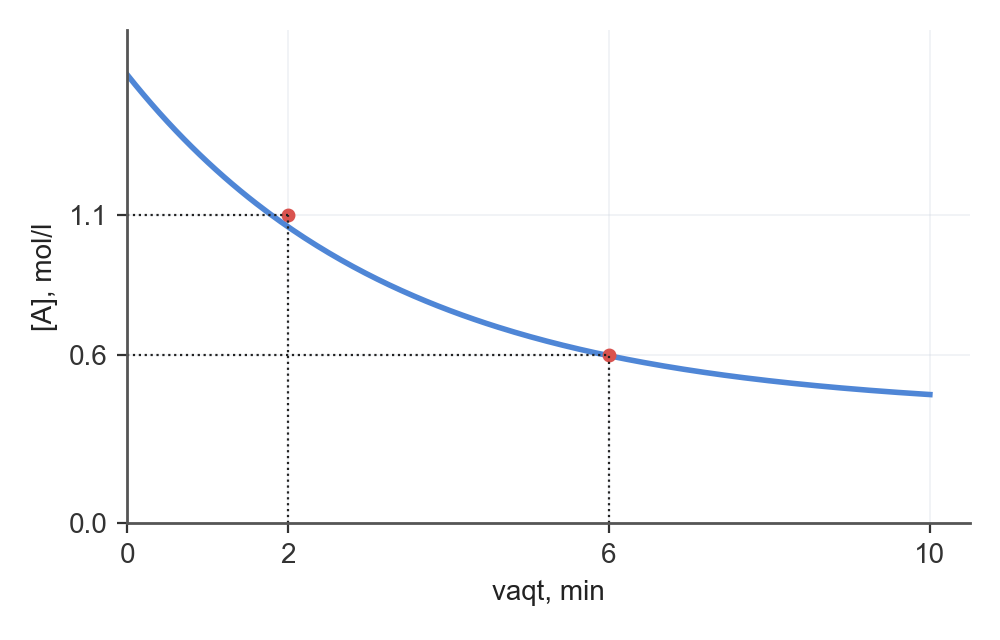
\includegraphics[width=0.86\linewidth]{rasmlar/gen/rate_v03_0.png}\end{center}
2-minutdan 6-minutgacha A moddaning konsentratsiyasi necha foizga kamaygan (2-minutdagiga nisbatan)?

\noindent A)~\textsl{54,5} \hfill B)~\textsl{83,3} \hfill C)~\textsl{45,5} \hfill D)~\textsl{50}\par
\qsep
\noindent\qn{9.} 9,6 g Mg va 14,6 g HCl aralashtirilib, reaksiya o`tkazildi (Mg + 2HCl $\to$ MgCl\textsubscript{2} + H\textsubscript{2}). Hosil bo`lgan MgCl\textsubscript{2} \textbf{massasini (g) aniqlang.}

\noindent A)~\textsl{38} \hfill B)~\textsl{9,5} \hfill C)~\textsl{19} \hfill D)~\textsl{28,5}\par
\qsep
\noindent\qn{10.} Quyidagi zarrachalardan qaysilari argon atomi bilan izoelektron? 1) Ca\textsuperscript{2+}; 2) F\textsuperscript{$-$}; 3) S\textsuperscript{2$-$}; 4) N\textsuperscript{3$-$}

\noindent A)~\textsl{1, 2, 4} \hfill B)~\textsl{1, 3} \hfill C)~\textsl{1, 2} \hfill D)~\textsl{2, 4}\par
\qsep
\noindent\qn{11.} CuSO\textsubscript{4} ning suvli eritmasi inert elektrodlar bilan elektroliz qilinganda qaysi moddalar ajraladi?

\noindent\begin{tabular}{@{}p{0.47\linewidth}@{}p{0.47\linewidth}@{}}
A)~\textsl{Ag va O\textsubscript{2}} & B)~\textsl{Zn, H\textsubscript{2} va O\textsubscript{2}} \\
C)~\textsl{H\textsubscript{2} va O\textsubscript{2}} & D)~\textsl{Cu va O\textsubscript{2}} \\
\end{tabular}\par
\qsep
\noindent\qn{12.} Jadvalda bog`lar hosil qiluvchi atomlarning elektrmanfiyliklari berilgan:
\begin{center}
\renewcommand{\arraystretch}{1.15}
\fitbox{\begin{tabular}{|c|c|c|}\hline
\textbf{Bog`} & \textbf{EM (1-atom)} & \textbf{EM (2-atom)} \\ \hline
H--O & 2,1 & 3,5 \\ \hline
C--H & 2,5 & 2,1 \\ \hline
H--Cl & 2,1 & 3 \\ \hline
Si--O & 1,8 & 3,5 \\ \hline
\end{tabular}}
\end{center}
Qaysi bog` eng qutbli (eng ko`p ionli xarakterga ega)?

\noindent A)~\textsl{H--O} \hfill B)~\textsl{C--H} \hfill C)~\textsl{Si--O} \hfill D)~\textsl{H--Cl}\par
\qsep
\noindent\qn{13.} 3 mol Ba(OH)\textsubscript{2} va 3 mol K\textsubscript{3}PO\textsubscript{4} suvda eritilib, eritma hajmi 2 l ga yetkazildi. Eritmadagi barcha ionlarning umumiy molyar \textbf{konsentratsiyasini (mol/l) aniqlang} (kuchli elektrolitlar to`liq dissotsilanadi).

\noindent A)~\textsl{3} \hfill B)~\textsl{10,5} \hfill C)~\textsl{21} \hfill D)~\textsl{5,25}\par
\qsep
\noindent\qn{14.} 4Fe(OH)\textsubscript{2} + O\textsubscript{2} + 2H\textsubscript{2}O $\to$ 4Fe(OH)\textsubscript{3} jarayoni uchun 22,5 g Fe(OH)\textsubscript{2} olingan. Fe(OH)\textsubscript{3} \textbf{massasini (g) aniqlang.}

\noindent A)~\textsl{53,5} \hfill B)~\textsl{13,38} \hfill C)~\textsl{26,75} \hfill D)~\textsl{40,12}\par
\qsep
\noindent\qn{15.} 0,02 mol Ca(HCO\textsubscript{3})\textsubscript{2} tutgan suv qaynatilganda ajralgan CO\textsubscript{2} hajmini (l, n.sh.)  \textbf{ni toping.}

\noindent A)~\textsl{0,9} \hfill B)~\textsl{0,45} \hfill C)~\textsl{0,22} \hfill D)~\textsl{0,67}\par
\qsep
\noindent\qn{16.} N\textsubscript{2}O\textsubscript{5} + H\textsubscript{2}O $\to$ 2HNO\textsubscript{3} jarayoni uchun 216 g N\textsubscript{2}O\textsubscript{5} olingan (unum 50\%). HNO\textsubscript{3} \textbf{miqdorini (mol) aniqlang.}

\noindent A)~\textsl{1} \hfill B)~\textsl{2} \hfill C)~\textsl{4} \hfill D)~\textsl{3}\par
\qsep
\noindent\qn{17.} Qaysi juftliklar o`zaro reaksiyaga kirishadi? 1) Ag va H\textsubscript{2}SO\textsubscript{4}(suyult.); 2) MgCl\textsubscript{2} va KNO\textsubscript{3}; 3) Fe va HCl; 4) Na\textsubscript{2}CO\textsubscript{3} va HCl

\noindent A)~\textsl{3, 4} \hfill B)~\textsl{1, 3} \hfill C)~\textsl{2, 3, 4} \hfill D)~\textsl{1, 2, 4}\par
\qsep
\noindent\qn{18.} Reaksiya tenglamasi: 2KCl + H\textsubscript{2}SO\textsubscript{4} $\to$ K\textsubscript{2}SO\textsubscript{4} + 2HCl. Reaksiyaga 49 g H\textsubscript{2}SO\textsubscript{4} kirishdi. HCl \textbf{hajmini (l, n.sh.) hisoblang.}

\noindent A)~\textsl{5,6} \hfill B)~\textsl{22,4} \hfill C)~\textsl{44,8} \hfill D)~\textsl{11,2}\par
\qsep
\noindent\qn{19.} NaNO\textsubscript{3} qizdirilganda qanday moddalar hosil bo`ladi?

\noindent\begin{tabular}{@{}p{0.47\linewidth}@{}p{0.47\linewidth}@{}}
A)~\textsl{KNO\textsubscript{2} va O\textsubscript{2}} & B)~\textsl{Ag, NO\textsubscript{2} va O\textsubscript{2}} \\
C)~\textsl{ZnO, NO\textsubscript{2} va O\textsubscript{2}} & D)~\textsl{NaNO\textsubscript{2} va O\textsubscript{2}} \\
\end{tabular}\par
\qsep
\noindent\qn{20.} CH\textsubscript{3}--CO--CH\textsubscript{2}--CH\textsubscript{3} birikmaning sistematik nomi qaysi qatorda to`g`ri keltirilgan?

\noindent A)~\textsl{butanon} \hfill B)~\textsl{butanal} \hfill C)~\textsl{butanol-2} \hfill D)~\textsl{propanon}\par
\qsep
\noindent\qn{21.} Etilen va asetilendan iborat 5,4 g aralashma mo`l bromli suv bilan to`liq reaksiyaga kirishdi. Sarflangan brom \textbf{massasini (g) aniqlang.} Aralashmadagi etilen va asetilenning mol nisbati 1 : 1.

\noindent A)~\textsl{48} \hfill B)~\textsl{96} \hfill C)~\textsl{24} \hfill D)~\textsl{32}\par
\qsep
\noindent\qn{22.} 39 g benzoldan nitrobenzol olishda unum 75\% bo`lsa, mahsulot \textbf{massasini (g) aniqlang.}

\noindent A)~\textsl{61,5} \hfill B)~\textsl{92,25} \hfill C)~\textsl{29,25} \hfill D)~\textsl{46,12}\par
\qsep
\noindent\qn{23.} Rasmdagi zanjirda CH\textsubscript{3}COOC\textsubscript{2}H\textsubscript{5} dan CH\textsubscript{3}COONa olish uchun \textit{X} reagent va \textbf{sharoitni aniqlang.}
\begin{center}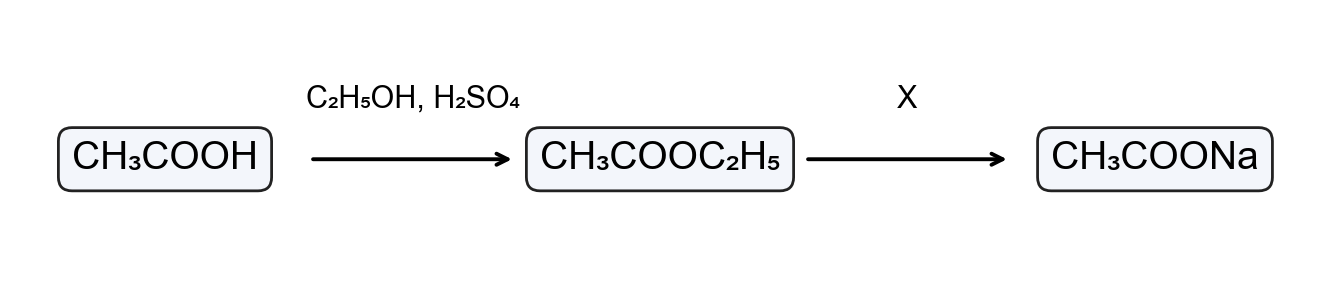
\includegraphics[width=0.86\linewidth]{rasmlar/gen/co_924866.png}\end{center}

\noindent\begin{tabular}{@{}p{0.47\linewidth}@{}p{0.47\linewidth}@{}}
A)~\textsl{H\textsubscript{2}SO\textsubscript{4} (kons.), 170 \textdegree{}C} & B)~\textsl{H\textsubscript{2}, kat.} \\
C)~\textsl{NaOH} & D)~\textsl{Br\textsubscript{2}} \\
\end{tabular}\par
\qsep
\noindent\qn{24.} Aldegid va ketonlar haqida qaysi fikrlar to`g`ri? 1) Aldegidlar qaytarilganda ikkilamchi spirt hosil bo`ladi; 2) Aseton Cu(OH)\textsubscript{2} ni qaytaradi; 3) Aseton suvda erimaydi; 4) Sirka aldegid Kucherov reaksiyasi bilan olinadi

\noindent A)~\textsl{1, 3} \hfill B)~\textsl{3} \hfill C)~\textsl{4} \hfill D)~\textsl{1}\par
\qsep
\noindent\qn{25.} Karbon kislotalar haqida qaysi fikrlar to`g`ri? 1) Sirka kislota karbonatlar bilan CO\textsubscript{2} ajratadi; 2) Karboksil guruh karbonil va gidroksil guruhlardan iborat; 3) Chumoli kislota "kumush ko`zgu" reaksiyasini beradi; 4) Olein kislota Br\textsubscript{2} ni biriktiradi

\noindent\begin{tabular}{@{}p{0.47\linewidth}@{}p{0.47\linewidth}@{}}
A)~\textsl{2, 3, 4} & B)~\textsl{1, 2, 3} \\
C)~\textsl{1, 3, 4} & D)~\textsl{1, 2, 3, 4} \\
\end{tabular}\par
\qsep
\noindent\qn{26.} 14,8 g CH\textsubscript{3}COOCH\textsubscript{3} mo`l NaOH bilan to`liq gidrolizlandi. Hosil bo`lgan tuz \textbf{massasini (g) aniqlang.}

\noindent A)~\textsl{16,4} \hfill B)~\textsl{14,8} \hfill C)~\textsl{32,8} \hfill D)~\textsl{8,2}\par
\qsep
\noindent\qn{27.} 36 g C\textsubscript{6}H\textsubscript{12}O\textsubscript{6} dan quyidagi ikki bosqichda C\textsubscript{2}H\textsubscript{5}ONa olinadi: 1) C\textsubscript{6}H\textsubscript{12}O\textsubscript{6} $\to$ 2C\textsubscript{2}H\textsubscript{5}OH + 2CO\textsubscript{2} (unum 75\%); 2) 2C\textsubscript{2}H\textsubscript{5}OH + 2Na $\to$ 2C\textsubscript{2}H\textsubscript{5}ONa + H\textsubscript{2} (unum 90\%). Oxirgi mahsulot C\textsubscript{2}H\textsubscript{5}ONa ning \textbf{massasini (g) toping.}

\noindent A)~\textsl{24,48} \hfill B)~\textsl{20,4} \hfill C)~\textsl{27,2} \hfill D)~\textsl{18,36}\par
\qsep
\noindent\qn{28.} 0,4 mol CH\textsubscript{3}NH\textsubscript{2} to`liq yondirilganda hosil bo`lgan CO\textsubscript{2} va N\textsubscript{2} hajmlari \textbf{yig`indisini (l, n.sh.) aniqlang} (4CH\textsubscript{3}NH\textsubscript{2} + 9O\textsubscript{2} $\to$ 4CO\textsubscript{2} + 10H\textsubscript{2}O + 2N\textsubscript{2}).

\noindent A)~\textsl{8,96} \hfill B)~\textsl{13,44} \hfill C)~\textsl{17,92} \hfill D)~\textsl{4,48}\par
\qsep
\noindent\qn{29.} Izobutilen monomeridan olingan polimerning polimerlanish darajasi 2000 bo`lsa, uning molyar \textbf{massasini (g/mol) aniqlang.}

\noindent A)~\textsl{56000} \hfill B)~\textsl{224000} \hfill C)~\textsl{112000} \hfill D)~\textsl{2056}\par
\qsep
\noindent\qn{30.} Metiloranj indikatori ishqoriy muhitda qanday rang beradi?

\noindent A)~\textsl{sariq} \hfill B)~\textsl{rangsiz} \hfill C)~\textsl{qizil} \hfill D)~\textsl{ko`k}\par
\qsep
\noindent\qn{31.} Rasmdagi asbob bilan qaysi aralashmani ajratish mumkin?
\begin{center}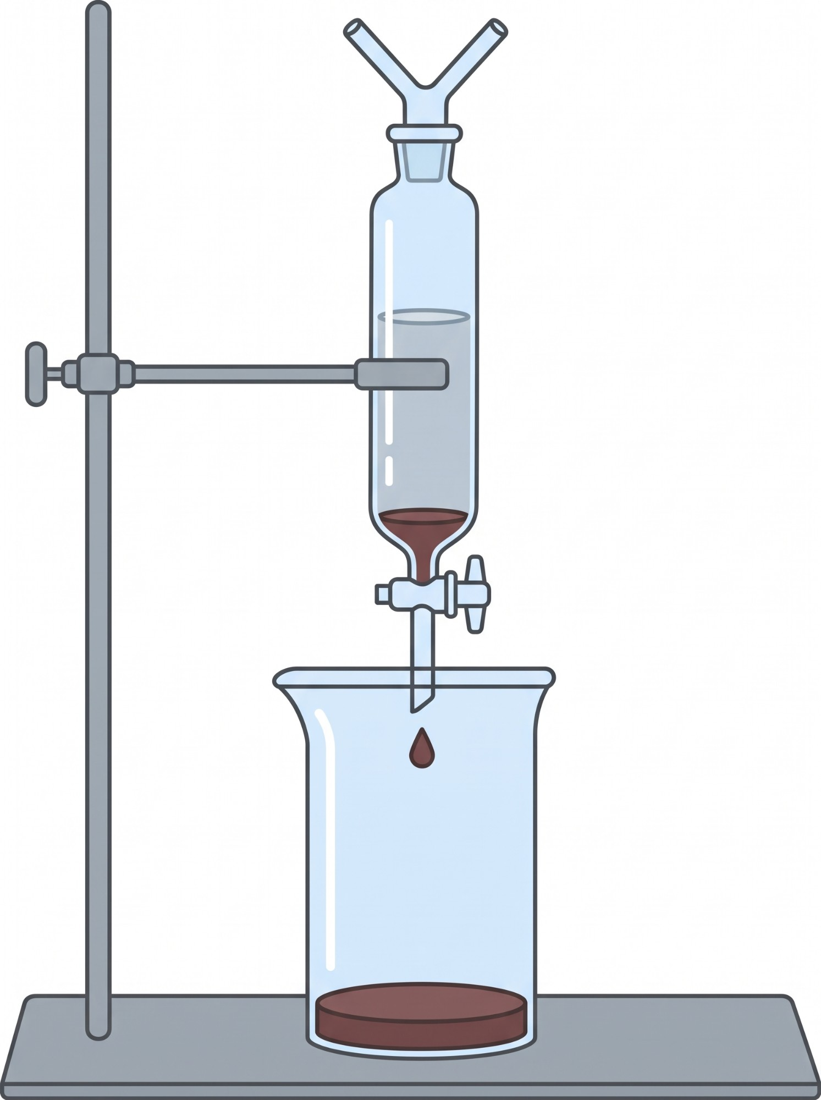
\includegraphics[width=0.86\linewidth]{rasmlar/darslik/d_ajratgich.png}\end{center}

\noindent\begin{tabular}{@{}p{0.47\linewidth}@{}p{0.47\linewidth}@{}}
A)~\textsl{suv va kerosin} & B)~\textsl{suv va etanol} \\
C)~\textsl{osh tuzi eritmasi} & D)~\textsl{suv va qum} \\
\end{tabular}\par
\qsep
\noindent\qn{32.} Laboratoriyada etilen olish uchun qaysi moddalar ishlatiladi?
\noindent A)~\textsl{FeS + HCl}\par
\noindent B)~\textsl{CaC\textsubscript{2} + H\textsubscript{2}O}\par
\noindent C)~\textsl{C\textsubscript{2}H\textsubscript{5}OH + H\textsubscript{2}SO\textsubscript{4} (kons.), 170 \textdegree{}C}\par
\noindent D)~\textsl{CH\textsubscript{3}COONa + NaOH (qizdirish)   ---}\par
\qsep
\end{multicols}
\medskip
\noindent\setlength{\fboxsep}{0pt}\fbox{\begin{tabular}{p{0.74\linewidth}|p{0.2\linewidth}}
\parbox[t]{0.72\linewidth}{\vspace{3pt}\textbf{Topshiriqlar (33--35) va javob variant (A--F)larini o`zaro to`g`ri moslashtiring.} Al va Al\textsubscript{2}O\textsubscript{3} dan iborat 12,9 g aralashma mo`l xlorid kislotada eritilganda 3,36 l (n.sh.) vodorod ajraldi.
\vspace{3pt}} & \parbox[t]{0.19\linewidth}{\vspace{3pt}A~\textsl{10,2}\\[3pt]
B~\textsl{164,25}\\[3pt]
C~\textsl{328,5}\\[3pt]
D~\textsl{60,08}\\[3pt]
E~\textsl{20,03}\\[3pt]
F~\textsl{40,05}}\\ \hline
\parbox[t]{0.72\linewidth}{\vspace{2pt}\textbf{33. Aralashmadagi Al\textsubscript{2}O\textsubscript{3} massasini (g) aniqlang.}\vspace{2pt}} & \\ \hline
\parbox[t]{0.72\linewidth}{\vspace{2pt}\textbf{34. Aralashmani eritish uchun sarflangan 20\% li HCl eritmasining massasini (g) aniqlang (M(HCl) = 36,5 g/mol).}\vspace{2pt}} & \\ \hline
\parbox[t]{0.72\linewidth}{\vspace{2pt}\textbf{35. Hosil bo`lgan AlCl\textsubscript{3} massasini (g) aniqlang.}\vspace{2pt}} & 
\end{tabular}}
\par\bigskip
\noindent\qn{36.} Cu + H\textsubscript{2}SO\textsubscript{4} $\to$ CuSO\textsubscript{4} + SO\textsubscript{2} + H\textsubscript{2}O reaksiya tenglamasini tenglang. Oksidlovchi va qaytaruvchi oldidagi koeffitsiyentlar \textbf{yig`indisini aniqlang.}
\javob\qsep
\noindent\qn{37.} Zichligi 1,12 g/ml bo`lgan 20\% li HNO\textsubscript{3} eritmasining molyar \textbf{konsentratsiyasini (mol/l) aniqlang.}
\javob\qsep
\noindent\qn{38.} 50 m\textsuperscript{3} suvda Ca(HCO\textsubscript{3})\textsubscript{2} konsentratsiyasi 10 mol/m\textsuperscript{3}, Mg(HCO\textsubscript{3})\textsubscript{2} niki 10 mol/m\textsuperscript{3}. Suvni Ca(OH)\textsubscript{2} bilan to`liq yumshatish uchun Ca(OH)\textsubscript{2} ning \textbf{massasini (kg) hisoblang.}
\javob\qsep
\noindent\qn{39.} Etilatsetat va metilatsetat dan iborat 25 g aralashma mo`l NaOH eritmasi bilan to`liq gidrolizlandi. Hosil bo`lgan spirtlar umumiy \textbf{massasini (g) toping.}
\javob\qsep
\noindent\qn{40.} To`yingan bir atomli aldegidning 7,2 g massasi Ag\textsubscript{2}O ning ammiakli eritmasi bilan oksidlanganda 21,6 g kumush ajraldi. Aldegidning molyar \textbf{massasini (g/mol) toping.}
\javob\qsep
\par\bigskip\begin{center}\textbf{\fontsize{13}{15}\selectfont YOZMA ISH}\end{center}
\noindent\qn{41.} \textbf{Topshiriqni bajarish jarayonida barcha reaksiya tenglamalarini yozing. Miqdoriy va arifmetik hisoblashlarni (unga asos bo`lgan usul yoki formulani ko`rsatgan holda) uzviy ketma-ketlikda bajaring.}\par\smallskip
HCOONa tuzining 1 mol/l li suvli eritmasi berilgan. HCOOH ning dissotsilanish konstantasi Ka = 1$\cdot$10\textsuperscript{$-$}4, K(suv) = 1$\cdot$10\textsuperscript{$-$14}.\par
\noindent 1)\ Tuzning gidrolizlanish reaksiyasi tenglamasini yozing va gidroliz konstantasini (Kh) hisoblang.\par
\noindent 2)\ Eritmadagi OH\textsuperscript{$-$} ionlarining konsentratsiyasini (mol/l) toping. pOH ni ham hisoblang.\par
\noindent 3)\ Eritmaning pH ini hisoblang.\par
\noindent 4)\ Gidrolizlanish darajasini (\%) aniqlang. Eritmadagi H\textsuperscript{+} konsentratsiyasini (mol/l) ham toping.\par
\noindent 5)\ Shunday eritmadan 500 ml tayyorlash uchun necha gramm HCOONa kerak? Eritma 10 marta suyultirilsa gidrolizlanish darajasi necha marta ortadi?\par
\diqqat{Mazkur topshiriq kengaytirilgan javobni talab etib, uning yechilish usuli va shu usul asosidagi barcha hisoblash amallari javoblar varaqasida aks etishi lozim.}\qsep
\noindent\qn{42.} Quyidagi o`zgarishlar zanjirida \textit{X}, \textit{Y}, \textit{Z} noma'lum organik moddalar:\par
\[\setlength{\fboxsep}{0pt}\text{CH\textsubscript{3}COOC\textsubscript{2}H\textsubscript{5}}\xrightarrow{\text{NaOH}}\text{\textit{X}}\xrightarrow{\text{NaOH (suyuqlanma), t\textdegree{}}}\text{\textit{Y}}\xrightarrow{\text{Cl\textsubscript{2}, yorug`lik}}\text{CH\textsubscript{3}Cl}\]
\noindent 1)\ CH\textsubscript{3}COOC\textsubscript{2}H\textsubscript{5} $\to$ \textit{X} : reaksiya tenglamasini yozing; hosil bo`lgan moddani nomlang.\par
\noindent 2)\ \textit{X} $\to$ \textit{Y} : reaksiya tenglamasini yozing; hosil bo`lgan moddani nomlang.\par
\noindent 3)\ \textit{Y} $\to$ CH\textsubscript{3}Cl : reaksiya tenglamasini yozing; hosil bo`lgan moddani nomlang.\par
\diqqat{Mazkur topshiriq kengaytirilgan javobni talab etib, uning yechilish usuli va shu usul asosidagi barcha hisoblash amallari javoblar varaqasida aks etishi lozim.}\qsep
\noindent\qn{43.} \textbf{Topshiriqni bajarish jarayonida barcha reaksiya tenglamalarini yozing. Miqdoriy va arifmetik hisoblashlarni (unga asos bo`lgan usul yoki formulani ko`rsatgan holda) uzviy ketma-ketlikda bajaring.}\par\smallskip
Uch probirkada XCl\textsubscript{2}, YCl\textsubscript{2} va ZCl\textsubscript{2} tarkibli metall xloridlarining eritmalari bor. Har bir eritmaga reagentlar ta'sir ettirildi, kuzatuvlar jadvalda ("---" belgisi reaksiya bormasligini bildiradi, bo`sh kataklar bo`yicha ma'lumot berilmagan):\par
\begin{center}
\renewcommand{\arraystretch}{1.15}
\begin{tabular}{|c|c|c|c|}\hline
\textbf{Reagent} & \textbf{XCl\textsubscript{2}} & \textbf{YCl\textsubscript{2}} & \textbf{ZCl\textsubscript{2}} \\ \hline
H\textsubscript{2}S & qora cho`kma & --- &  \\ \hline
Na\textsubscript{2}S & qora cho`kma & qora cho`kma & oq cho`kma \\ \hline
NaOH & havorang cho`kma & och yashil cho`kma & oq cho`kma \\ \hline
Zn plastinka & qizil qoplama &  & --- \\ \hline
\end{tabular}
\end{center}
\textit{X}, \textit{Y}, \textit{Z} --- davriy sistemaning to`rtinchi davridagi metallar.\par
\noindent 1)\ Jadvalda kuzatilgan barcha reaksiyalarning molekulyar tenglamalarini yozing. XCl\textsubscript{2} eritmasiga tushirilgan Zn plastinkada 0,1 mol \textit{X} ajralgan bo`lsa, plastinka massasi qanchaga (g) o`zgargan?\par
\noindent 2)\ \textit{X}, \textit{Y}, \textit{Z} metallarni aniqlang va tuzlarning formulalarini yozing. XCl\textsubscript{2} tarkibida \textit{X} ning massa ulushi 47,4\% ekanini hisob bilan tasdiqlang.\par
\noindent 3)\ 25,4 g YCl\textsubscript{2} eritmasiga mo`l NaOH qo`shildi, hosil bo`lgan cho`kma havoda to`liq oksidlanguncha qoldirildi. Barcha reaksiya tenglamalarini yozing va oxirgi cho`kma massasini (g) aniqlang.\par
\noindent 4)\ ZCl\textsubscript{2} ning 13,6 g massasi mo`l NaOH eritmasi bilan reaksiyaga kirishganda hosil bo`lgan kompleks tuz massasini (g) hisoblang (reaksiya tenglamalarini yozing).\par
\noindent 5)\ Hosil bo`lgan Cu(OH)\textsubscript{2} cho`kmasi (0,1 mol) qizdirilganda hosil bo`ladigan CuO massasini (g) hisoblang.\par
\diqqat{Mazkur topshiriq kengaytirilgan javobni talab etib, uning yechilish usuli va shu usul asosidagi barcha hisoblash amallari javoblar varaqasida aks etishi lozim.}\qsep
\newpage
\renewcommand{\curvar}{4-variant}
\thispagestyle{first}
\noindent\textit{Davriy jadvaldan foydalanish mumkin.}
\par\smallskip
\begin{multicols}{2}
\noindent\qn{1.} A moddaning parchalanish reaksiyasida konsentratsiyaning vaqt bo`yicha o`zgarishi jadvalda berilgan:
\begin{center}
\renewcommand{\arraystretch}{1.15}
\fitbox{\begin{tabular}{|c|c|}\hline
\textbf{t, min} & \textbf{c, mol/l} \\ \hline
0 & 1,6 \\ \hline
2 & 1,44 \\ \hline
4 & 1,28 \\ \hline
6 & 1,12 \\ \hline
\end{tabular}}
\end{center}
2-minutdan 6-minutgacha o`rtacha tezlikni mol/(l$\cdot$min) \textbf{hisoblang.}

\noindent A)~\textsl{0,16} \hfill B)~\textsl{0,08} \hfill C)~\textsl{0,04} \hfill D)~\textsl{0,32}\par
\qsep
\noindent\qn{2.} Mo`l kislota bilan Zn ning turli massalari ta'sirlashganda ajralgan H\textsubscript{2} hajmi grafikda keltirilgan (n.sh.).
\begin{center}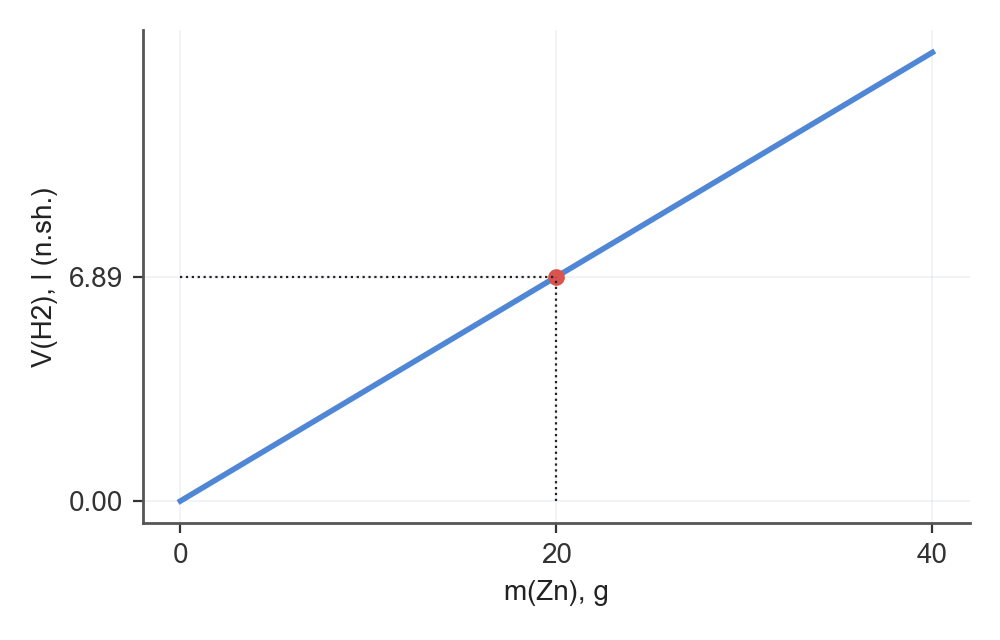
\includegraphics[width=0.86\linewidth]{rasmlar/gen/li_v04_0.png}\end{center}
Zn ning molyar massasini (g/mol) grafikdan \textbf{aniqlang.}

\noindent A)~\textsl{130} \hfill B)~\textsl{32,5} \hfill C)~\textsl{65} \hfill D)~\textsl{87,4}\par
\qsep
\noindent\qn{3.} 17-tartib raqamli elementning barcha elektronlaridan nechtasining spin kvant soni m\_s = +$\frac{1}{2}$ ga teng (Hund qoidasi bo`yicha to`ldirilgan holat)?

\noindent A)~\textsl{9} \hfill B)~\textsl{10} \hfill C)~\textsl{8} \hfill D)~\textsl{11}\par
\qsep
\noindent\qn{4.} 10 l CO va 7,5 l O\textsubscript{2} aralashmasi reaksiyaga kirishdi (2CO + O\textsubscript{2} $\to$ 2CO\textsubscript{2}, hamma moddalar bir xil sharoitda gaz holida). Reaksiyadan keyingi gaz aralashmasining \textbf{hajmini (l) aniqlang.}

\noindent A)~\textsl{17,5} \hfill B)~\textsl{12,5} \hfill C)~\textsl{10} \hfill D)~\textsl{2,5}\par
\qsep
\noindent\qn{5.} HNO\textsubscript{2} tarkibida N ning oksidlanish \textbf{darajasini aniqlang.}

\noindent A)~\textsl{$-$3} \hfill B)~\textsl{+2} \hfill C)~\textsl{$-$3 va +5} \hfill D)~\textsl{+3}\par
\qsep
\noindent\qn{6.} \textit{X}\textsuperscript{3+} ionida 10 ta elektron va 16 ta neytron bor. \textit{X} atomining nisbiy atom \textbf{massasini aniqlang.}

\noindent A)~\textsl{29} \hfill B)~\textsl{32} \hfill C)~\textsl{26} \hfill D)~\textsl{13}\par
\qsep
\noindent\qn{7.} 2SO\textsubscript{2} + O\textsubscript{2} $\rightleftarrows$ 2SO\textsubscript{3} reaksiyada muvozanat qaror topganda [SO\textsubscript{2}] = 0,5, [O\textsubscript{2}] = 3, [SO\textsubscript{3}] = 2 mol/l bo`ldi. SO\textsubscript{2} ning boshlang`ich \textbf{konsentratsiyasini (mol/l) aniqlang.}

\noindent A)~\textsl{0,5} \hfill B)~\textsl{3,5} \hfill C)~\textsl{2,5} \hfill D)~\textsl{1,5}\par
\qsep
\noindent\qn{8.} CaCO\textsubscript{3} $\rightleftarrows$ CaO + CO\textsubscript{2} -- Q muvozanatni o`ngga siljitadigan \textbf{o`zgarishlarni toping}: 1) haroratni pasaytirish; 2) bosimni oshirish; 3) bosimni pasaytirish; 4) haroratni oshirish.

\noindent A)~\textsl{1, 3, 4} \hfill B)~\textsl{1, 2} \hfill C)~\textsl{3, 4} \hfill D)~\textsl{1, 3}\par
\qsep
\noindent\qn{9.} Na\textsubscript{2}SO\textsubscript{4}$\cdot$10H\textsubscript{2}O kristallogidratida kristallizatsion suvning massa \textbf{ulushini (\%) aniqlang.}

\noindent A)~\textsl{44,1} \hfill B)~\textsl{55,9} \hfill C)~\textsl{28} \hfill D)~\textsl{126,8}\par
\qsep
\noindent\qn{10.} CuCl\textsubscript{2} eritmasi inert elektrodlar yordamida 10 A tok kuchi bilan 9650 s elektroliz qilindi. Katodda ajralgan Cu massasi (g) \textbf{ni toping.}

\noindent A)~\textsl{64} \hfill B)~\textsl{32} \hfill C)~\textsl{16} \hfill D)~\textsl{48}\par
\qsep
\noindent\qn{11.} Zarracha haqida ma'lumot jadvalda berilgan:
\begin{center}
\renewcommand{\arraystretch}{1.15}
\fitbox{\begin{tabular}{|c|c|}\hline
\textbf{Zarracha tarkibi} & \textbf{Soni} \\ \hline
proton & 16 \\ \hline
neytron & 17 \\ \hline
elektron & 17 \\ \hline
\end{tabular}}
\end{center}
Shu zarrachaning massa \textbf{sonini aniqlang.}

\noindent A)~\textsl{34} \hfill B)~\textsl{32} \hfill C)~\textsl{33} \hfill D)~\textsl{35}\par
\qsep
\noindent\qn{12.} Qaysi juftliklarda reaksiya bormaydi? 1) Fe va MgCl\textsubscript{2}; 2) Zn va CuSO\textsubscript{4}; 3) Al va CuSO\textsubscript{4}; 4) Cu va ZnSO\textsubscript{4}

\noindent A)~\textsl{1, 4} \hfill B)~\textsl{3, 4} \hfill C)~\textsl{1, 2} \hfill D)~\textsl{4}\par
\qsep
\noindent\qn{13.} Zichligi 1,15 g/ml bo`lgan 30\% li HCl eritmasining molyar \textbf{konsentratsiyasini (mol/l) aniqlang.}

\noindent A)~\textsl{9,45} \hfill B)~\textsl{0,95} \hfill C)~\textsl{18,9} \hfill D)~\textsl{8,22}\par
\qsep
\noindent\qn{14.} Qaysi juftliklar o`zaro reaksiyaga kirishadi? 1) CuSO\textsubscript{4} va NaOH; 2) Zn va NaOH; 3) MgCl\textsubscript{2} va KNO\textsubscript{3}; 4) Cu va HNO\textsubscript{3}(kons.)

\noindent A)~\textsl{1, 4} \hfill B)~\textsl{1, 2, 4} \hfill C)~\textsl{1, 3} \hfill D)~\textsl{2, 3, 4}\par
\qsep
\noindent\qn{15.} 2KClO\textsubscript{3} $\to$ 2KCl + 3O\textsubscript{2} reaksiyasida 245 g KClO\textsubscript{3} ishtirok etdi. O\textsubscript{2} \textbf{hajmini (l, n.sh.) toping.}

\noindent A)~\textsl{29,87} \hfill B)~\textsl{67,2} \hfill C)~\textsl{134,4} \hfill D)~\textsl{33,6}\par
\qsep
\noindent\qn{16.} K\textsubscript{2}SO\textsubscript{4} tarkibidagi kaliy ning massa \textbf{ulushini (\%) aniqlang.}

\noindent A)~\textsl{22,4} \hfill B)~\textsl{89,7} \hfill C)~\textsl{2,2} \hfill D)~\textsl{44,8}\par
\qsep
\noindent\qn{17.} AgNO\textsubscript{3} qizdirilganda qanday moddalar hosil bo`ladi?

\noindent\begin{tabular}{@{}p{0.47\linewidth}@{}p{0.47\linewidth}@{}}
A)~\textsl{CuO, NO\textsubscript{2} va O\textsubscript{2}} & B)~\textsl{KNO\textsubscript{2} va O\textsubscript{2}} \\
C)~\textsl{ZnO, NO\textsubscript{2} va O\textsubscript{2}} & D)~\textsl{Ag, NO\textsubscript{2} va O\textsubscript{2}} \\
\end{tabular}\par
\qsep
\noindent\qn{18.} Reaksiya tenglamasi: FeS + 2HCl $\to$ FeCl\textsubscript{2} + H\textsubscript{2}S. Reaksiyaga 11,2 l (n.sh.) HCl kirishdi. FeCl\textsubscript{2} \textbf{massasini (g) hisoblang.}

\noindent A)~\textsl{31,75} \hfill B)~\textsl{127} \hfill C)~\textsl{63,5} \hfill D)~\textsl{15,88}\par
\qsep
\noindent\qn{19.} Reaksiya tenglamasi: NH\textsubscript{4}Cl + NaOH $\to$ NaCl + NH\textsubscript{3} + H\textsubscript{2}O. Reaksiyaga tarkibida 60\% aralashma bo`lgan 40 g namuna (asosiy modda NaOH) kirishdi. NH\textsubscript{3} \textbf{hajmini (l, n.sh.) hisoblang.}

\noindent A)~\textsl{8,96} \hfill B)~\textsl{17,92} \hfill C)~\textsl{4,48} \hfill D)~\textsl{13,44}\par
\qsep
\noindent\qn{20.} Rasmda $\alpha$-aminokislotaning tuzilish formulasi berilgan.
\begin{center}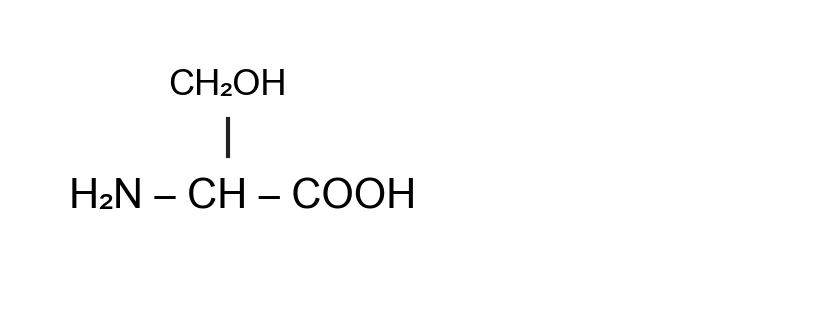
\includegraphics[width=0.86\linewidth]{rasmlar/gen/aa_999520.png}\end{center}
Aminokislotaning \textbf{nomini toping.}

\noindent A)~\textsl{alanin} \hfill B)~\textsl{serin} \hfill C)~\textsl{glitsin} \hfill D)~\textsl{valin}\par
\qsep
\noindent\qn{21.} Alken, alkadiyen va alkinlar haqida qaysi fikrlar to`g`ri? 1) Alkenlarda $\pi$-bog` yo`q; 2) Alkinlar uchun umumiy formula CnH\textsubscript{2}n+2; 3) Kauchuk izoprenning polimeri; 4) Etilen sanoatda kreking gazlaridan olinadi

\noindent A)~\textsl{1, 2, 4} \hfill B)~\textsl{1, 2, 3} \hfill C)~\textsl{1, 3} \hfill D)~\textsl{3, 4}\par
\qsep
\noindent\qn{22.} Arenlar, neft va tabiiy gaz haqida qaysi fikrlar to`g`ri? 1) Benzol bromli suvni rangsizlantirmaydi; 2) Benzoldan nitrobenzol nitrolash bilan olinadi; 3) Neft fraksiyalaridan gazolin 150 \textdegree{}C gacha haydaladi; 4) Naftalin -- bir halqali aren

\noindent A)~\textsl{3, 4} \hfill B)~\textsl{1, 2, 4} \hfill C)~\textsl{1, 3} \hfill D)~\textsl{1, 2, 3}\par
\qsep
\noindent\qn{23.} Spirt va fenollar haqida qaysi fikrlar to`g`ri? 1) Fenol FeCl\textsubscript{3} bilan binafsha rang beradi; 2) Uchlamchi spirtlar oson oksidlanadi; 3) Fenol Cu(OH)\textsubscript{2} ni eritib ko`k kompleks hosil qiladi; 4) Glitserin Cu(OH)\textsubscript{2} bilan ko`k kompleks hosil qiladi

\noindent A)~\textsl{1, 2, 3} \hfill B)~\textsl{1, 3, 4} \hfill C)~\textsl{1, 3} \hfill D)~\textsl{1, 4}\par
\qsep
\noindent\qn{24.} 44 g CH\textsubscript{3}CHO dan quyidagi ikki bosqichda (CH\textsubscript{3}COO)\textsubscript{2}Ca olinadi: 1) CH\textsubscript{3}CHO + 2Cu(OH)\textsubscript{2} $\to$ CH\textsubscript{3}COOH + Cu\textsubscript{2}O + 2H\textsubscript{2}O (unum 60\%); 2) 2CH\textsubscript{3}COOH + CaCO\textsubscript{3} $\to$ (CH\textsubscript{3}COO)\textsubscript{2}Ca + CO\textsubscript{2} + H\textsubscript{2}O (unum 90\%). Oxirgi mahsulot (CH\textsubscript{3}COO)\textsubscript{2}Ca ning \textbf{massasini (g) toping.}

\noindent A)~\textsl{71,1} \hfill B)~\textsl{47,4} \hfill C)~\textsl{79} \hfill D)~\textsl{42,66}\par
\qsep
\noindent\qn{25.} Karbon kislotalar haqida qaysi fikrlar to`g`ri? 1) Sirka kislota karbonatlar bilan CO\textsubscript{2} ajratadi; 2) Qattiq suvda sovun yaxshi ko`piklanadi; 3) Benzoy kislota Na\textsubscript{2}CO\textsubscript{3} bilan reaksiyaga kirishmaydi; 4) Chumoli kislota "kumush ko`zgu" reaksiyasini beradi

\noindent A)~\textsl{3, 4} \hfill B)~\textsl{1, 3} \hfill C)~\textsl{1, 4} \hfill D)~\textsl{2, 3}\par
\qsep
\noindent\qn{26.} CH\textsubscript{3}COOCH\textsubscript{3} + NaOH $\to$ CH\textsubscript{3}COONa + CH\textsubscript{3}OH jarayoni uchun 20 g NaOH olingan (unum 90\%). CH\textsubscript{3}COONa \textbf{massasini (g) aniqlang.}

\noindent A)~\textsl{41} \hfill B)~\textsl{73,8} \hfill C)~\textsl{36,9} \hfill D)~\textsl{18,45}\par
\qsep
\noindent\qn{27.} Quyidagi birikmalardan qaysi biri spirt sinfiga kiradi?

\noindent\begin{tabular}{@{}p{0.47\linewidth}@{}p{0.47\linewidth}@{}}
A)~\textsl{CH\textsubscript{3}COOH} & B)~\textsl{C\textsubscript{6}H\textsubscript{5}NH\textsubscript{2}} \\
C)~\textsl{C\textsubscript{2}H\textsubscript{5}OH} & D)~\textsl{CH\textsubscript{3}COOC\textsubscript{2}H\textsubscript{5}} \\
\end{tabular}\par
\qsep
\noindent\qn{28.} NH\textsubscript{2}CH\textsubscript{2}COOH + C\textsubscript{2}H\textsubscript{5}OH $\to$ NH\textsubscript{2}CH\textsubscript{2}COOC\textsubscript{2}H\textsubscript{5} + H\textsubscript{2}O reaksiyasida 46 g C\textsubscript{2}H\textsubscript{5}OH ishtirok etdi (unum 90\%). NH\textsubscript{2}CH\textsubscript{2}COOC\textsubscript{2}H\textsubscript{5} \textbf{massasini (g) toping.}

\noindent A)~\textsl{92,7} \hfill B)~\textsl{103} \hfill C)~\textsl{185,4} \hfill D)~\textsl{46,35}\par
\qsep
\noindent\qn{29.} Izopren monomeridan olingan polimerning molyar massasi 34000 g/mol. Polimerlanish \textbf{darajasini aniqlang.}

\noindent A)~\textsl{1000} \hfill B)~\textsl{500} \hfill C)~\textsl{250} \hfill D)~\textsl{510}\par
\qsep
\noindent\qn{30.} Ba\textsuperscript{2+} ionini aniqlash uchun qaysi reagent mos va qanday belgi kuzatiladi?
\noindent A)~\textsl{H\textsubscript{2}SO\textsubscript{4}: oq cho`kma (BaSO\textsubscript{4}), HCl da erimaydi}\par
\noindent B)~\textsl{AgNO\textsubscript{3}: sariq cho`kma (Ag\textsubscript{3}PO\textsubscript{4}), HNO\textsubscript{3} da eriydi}\par
\noindent C)~\textsl{AgNO\textsubscript{3}: och sariq cho`kma (AgBr)}\par
\noindent D)~\textsl{HCl: rangsiz gaz (CO\textsubscript{2}) ajraladi}\par
\qsep
\noindent\qn{31.} Uch probirkada (\textit{X}, \textit{Y}, \textit{Z}) glyukoza, saxaroza, kraxmal eritmalari bor (tartibsiz). Ularga yod va Cu(OH)\textsubscript{2} ta'sir ettirildi. Kuzatuvlar jadvalda:
\begin{center}
\renewcommand{\arraystretch}{1.15}
\fitbox{\begin{tabular}{|c|c|c|}\hline
\textbf{Probirka} & \textbf{I\textsubscript{2} eritmasi} & \textbf{Cu(OH)\textsubscript{2} (qizdirilganda)} \\ \hline
\textit{X} & o`zgarish yo`q & o`zgarish yo`q \\ \hline
\textit{Y} & o`zgarish yo`q & qizdirilganda qizil cho`kma \\ \hline
\textit{Z} & ko`k rang & o`zgarish yo`q \\ \hline
\end{tabular}}
\end{center}
\textit{X}, \textit{Y}, \textit{Z} probirkalardagi \textbf{moddalarni aniqlang.}
\noindent A)~\textsl{\textit{X} -- glyukoza, \textit{Y} -- saxaroza, \textit{Z} -- kraxmal}\par
\noindent B)~\textsl{\textit{X} -- glyukoza, \textit{Y} -- kraxmal, \textit{Z} -- saxaroza}\par
\noindent C)~\textsl{\textit{X} -- kraxmal, \textit{Y} -- saxaroza, \textit{Z} -- glyukoza}\par
\noindent D)~\textsl{\textit{X} -- saxaroza, \textit{Y} -- glyukoza, \textit{Z} -- kraxmal}\par
\qsep
\noindent\qn{32.} Rasmdagi asbobda sirka kislota va izoamil spirti konsentrlangan H\textsubscript{2}SO\textsubscript{4} ishtirokida qizdirilmoqda. Qanday modda hosil bo`ladi?
\begin{center}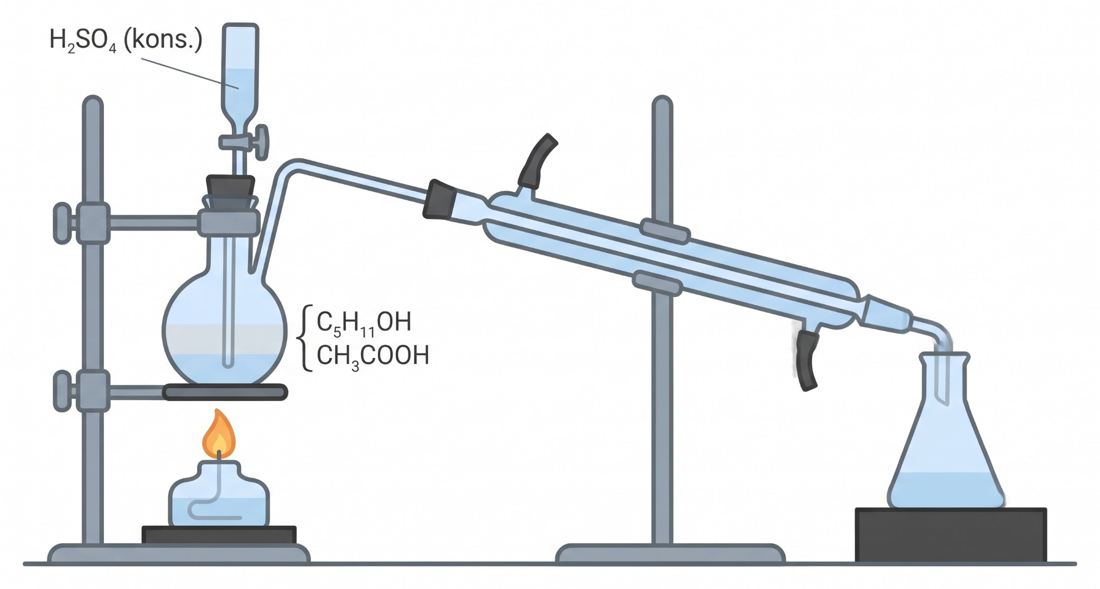
\includegraphics[width=0.86\linewidth]{rasmlar/darslik/d_efir.png}\end{center}
\noindent A)~\textsl{aldegid}\par
\noindent B)~\textsl{uglevod}\par
\noindent C)~\textsl{murakkab efir (izoamilasetat)}\par
\noindent D)~\textsl{oddiy efir   ---}\par
\qsep
\end{multicols}
\medskip
\noindent\setlength{\fboxsep}{0pt}\fbox{\begin{tabular}{p{0.74\linewidth}|p{0.2\linewidth}}
\parbox[t]{0.72\linewidth}{\vspace{3pt}\textbf{Topshiriqlar (33--35) va javob variant (A--F)larini o`zaro to`g`ri moslashtiring.} Propan (C\textsubscript{3}H\textsubscript{8}) va eten (C\textsubscript{2}H\textsubscript{4}) dan iborat 6,72 l (n.sh.) aralashma bromli suvdan o`tkazilganda 16 g brom yutildi.
\vspace{3pt}} & \parbox[t]{0.19\linewidth}{\vspace{3pt}A~\textsl{138,67}\\[3pt]
B~\textsl{208}\\[3pt]
C~\textsl{33,33}\\[3pt]
D~\textsl{2,24}\\[3pt]
E~\textsl{26,67}\\[3pt]
F~\textsl{3,36}}\\ \hline
\parbox[t]{0.72\linewidth}{\vspace{2pt}\textbf{33. Aralashmadagi eten (C\textsubscript{2}H\textsubscript{4}) hajmini (l, n.sh.) aniqlang.}\vspace{2pt}} & \\ \hline
\parbox[t]{0.72\linewidth}{\vspace{2pt}\textbf{34. Aralashmadagi eten (C\textsubscript{2}H\textsubscript{4}) hajmiy ulushini (\%) aniqlang.}\vspace{2pt}} & \\ \hline
\parbox[t]{0.72\linewidth}{\vspace{2pt}\textbf{35. Aralashmani to`liq yoqish uchun zarur havo hajmini (l, n.sh.; havoda 21\% kislorod bor) aniqlang.}\vspace{2pt}} & 
\end{tabular}}
\par\bigskip
\noindent\qn{36.} KMnO\textsubscript{4} + Na\textsubscript{2}SO\textsubscript{3} + H\textsubscript{2}O $\to$ MnO\textsubscript{2} + Na\textsubscript{2}SO\textsubscript{4} + KOH reaksiya tenglamasini tenglang. Oksidlovchi va qaytaruvchi oldidagi koeffitsiyentlar \textbf{yig`indisini aniqlang.}
\javob\qsep
\noindent\qn{37.} 1 l hajmli yopiq idishda 1 mol N\textsubscript{2}O\textsubscript{4} qizdirilganda N\textsubscript{2}O\textsubscript{4} $\rightleftarrows$ 2NO\textsubscript{2} muvozanati qaror topdi. Muvozanat aralashmasining vodorodga nisbatan zichligi 30,67 ga teng. Shu haroratdagi muvozanat \textbf{konstantasini (K, mol/l) hisoblang.}
\javob\qsep
\noindent\qn{38.} Alyuminiy va mis dan iborat 9,1 g aralashma mo`l NaOH eritmasida eritildi. Ajralgan gazning \textbf{hajmini (l, n.sh.) aniqlang} (mis ishqor bilan reaksiyaga kirishmaydi).
\javob\qsep
\noindent\qn{39.} 4,6 g etanol avval sirka aldegidgacha (unum 75\%), so`ng sirka kislotagacha (unum 60\%) oksidlandi; hosil bo`lgan kislota mo`l etanol bilan efirlandi (unum 100\%). Etilatsetat \textbf{massasini (g) toping.}
\javob\qsep
\noindent\qn{40.} Polipropilen polimerining (polimerlanish darajasi 2000) 168 g namunasini olish uchun polimerlanish unumi 90\% bo`lganda qancha monomer (C\textsubscript{3}H\textsubscript{6}) kerak (g)?
\javob\qsep
\par\bigskip\begin{center}\textbf{\fontsize{13}{15}\selectfont YOZMA ISH}\end{center}
\noindent\qn{41.} \textbf{Topshiriqni bajarish jarayonida barcha reaksiya tenglamalarini yozing. Miqdoriy va arifmetik hisoblashlarni (unga asos bo`lgan usul yoki formulani ko`rsatgan holda) uzviy ketma-ketlikda bajaring.}\par\smallskip
Laboratoriyada xlor olish uchun K\textsubscript{2}Cr\textsubscript{2}O\textsubscript{7} ga konsentrlangan xlorid kislota ta'sir ettirildi: K\textsubscript{2}Cr\textsubscript{2}O\textsubscript{7} + 14HCl $\to$ 2KCl + 2CrCl\textsubscript{3} + 3Cl\textsubscript{2} + 7H\textsubscript{2}O. Ajralgan 13,44 l (n.sh.) xlor gazining yarmi mo`l KI eritmasidan o`tkazildi, qolgan yarmi esa issiq mo`l KOH eritmasiga yuttirildi.\par
\noindent 1)\ Reaksiyani elektron balans usulida tenglang: oksidlovchi va qaytaruvchini ko`rsating, koeffitsiyentlar yig`indisini toping.\par
\noindent 2)\ K\textsubscript{2}Cr\textsubscript{2}O\textsubscript{7} ning sarflangan massasini (g) hisoblang. Sarflangan oksidlovchining miqdorini (mol) ham toping.\par
\noindent 3)\ Sarflangan HCl miqdorini (mol) va shundan qaytaruvchi sifatida ishtirok etgan qismini (mol) aniqlang.\par
\noindent 4)\ Xlor mo`l KI eritmasidan o`tkazilganda ajralgan yodning massasini (g) toping (reaksiya tenglamasini yozing). Sarflangan KI massasini (g) ham toping.\par
\noindent 5)\ Issiq KOH eritmasiga yuttirilganda (3Cl\textsubscript{2} + 6KOH $\to$ KClO\textsubscript{3} + 5KCl + 3H\textsubscript{2}O) hosil bo`lgan KClO\textsubscript{3} massasini (g) aniqlang. Agar xlor sovuq KOH eritmasiga yuttirilsa (Cl\textsubscript{2} + 2KOH $\to$ KCl + KClO + H\textsubscript{2}O), hosil bo`ladigan KClO massasini (g) ham toping.\par
\diqqat{Mazkur topshiriq kengaytirilgan javobni talab etib, uning yechilish usuli va shu usul asosidagi barcha hisoblash amallari javoblar varaqasida aks etishi lozim.}\qsep
\noindent\qn{42.} Quyidagi o`zgarishlar zanjirida \textit{X}, \textit{Y}, \textit{Z} noma'lum organik moddalar:\par
\[\setlength{\fboxsep}{0pt}\text{CaC\textsubscript{2}}\xrightarrow{\text{H\textsubscript{2}O}}\text{\textit{X}}\xrightarrow{\text{C (aktiv), 600 \textdegree{}C}}\text{\textit{Y}}\xrightarrow{\text{HNO\textsubscript{3}, H\textsubscript{2}SO\textsubscript{4}}}\text{\textit{Z}}\xrightarrow{\text{Fe, HCl}}\text{C\textsubscript{6}H\textsubscript{5}NH\textsubscript{2}}\]
\noindent 1)\ CaC\textsubscript{2} $\to$ \textit{X} : reaksiya tenglamasini yozing; hosil bo`lgan moddani nomlang.\par
\noindent 2)\ \textit{X} $\to$ \textit{Y} : reaksiya tenglamasini yozing; hosil bo`lgan moddani nomlang.\par
\noindent 3)\ \textit{Y} $\to$ \textit{Z} : reaksiya tenglamasini yozing; hosil bo`lgan moddani nomlang.\par
\noindent 4)\ \textit{Z} $\to$ C\textsubscript{6}H\textsubscript{5}NH\textsubscript{2} : reaksiya tenglamasini yozing; hosil bo`lgan moddani nomlang.\par
\diqqat{Mazkur topshiriq kengaytirilgan javobni talab etib, uning yechilish usuli va shu usul asosidagi barcha hisoblash amallari javoblar varaqasida aks etishi lozim.}\qsep
\noindent\qn{43.} \textbf{Topshiriqni bajarish jarayonida barcha reaksiya tenglamalarini yozing. Miqdoriy va arifmetik hisoblashlarni (unga asos bo`lgan usul yoki formulani ko`rsatgan holda) uzviy ketma-ketlikda bajaring.}\par\smallskip
33,1 g Pb(NO\textsubscript{3})\textsubscript{2} qizdirilganda qisman parchalandi va qattiq qoldiq massasi 30,4 g bo`ldi. Ajralgan gazlar aralashmasi 300 g suvga to`liq yuttirildi. Qattiq qoldiqdagi PbO esa mo`l suyultirilgan H\textsubscript{2}SO\textsubscript{4} bilan reaksiyaga kiritildi.\par
\noindent 1)\ Parchalanish reaksiyasi tenglamasini yozing. Parchalangan Pb(NO\textsubscript{3})\textsubscript{2} ning ulushini (\%) va ajralgan gazlar umumiy hajmini (l, n.sh.) aniqlang.\par
\noindent 2)\ Qattiq qoldiqdagi PbO ning massa ulushini (\%) hisoblang.\par
\noindent 3)\ Gazlar suvga yuttirilganda hosil bo`lgan eritmadagi HNO\textsubscript{3} ning massa ulushini (\%) toping (reaksiya tenglamasini yozing).\par
\noindent 4)\ Qoldiqdagi PbO ni to`liq eritish uchun 20\% li H\textsubscript{2}SO\textsubscript{4} eritmasidan necha gramm kerak va hosil bo`lgan PbSO\textsubscript{4} ning massasi qancha?\par
\noindent 5)\ Ajralgan NO\textsubscript{2} va O\textsubscript{2} gazlari aralashmasining o`rtacha molyar massasini (g/mol) hisoblang.\par
\diqqat{Mazkur topshiriq kengaytirilgan javobni talab etib, uning yechilish usuli va shu usul asosidagi barcha hisoblash amallari javoblar varaqasida aks etishi lozim.}\qsep
\newpage
\renewcommand{\curvar}{5-variant}
\thispagestyle{first}
\noindent\textit{Davriy jadvaldan foydalanish mumkin.}
\par\smallskip
\begin{multicols}{2}
\noindent\qn{1.} Quyidagi tuzlarning qaysilari suvli eritmasi kislotali muhitga ega? 1) CH\textsubscript{3}COONa; 2) Na\textsubscript{2}SO\textsubscript{4}; 3) FeCl\textsubscript{3}; 4) Na\textsubscript{2}CO\textsubscript{3}

\noindent A)~\textsl{2} \hfill B)~\textsl{3} \hfill C)~\textsl{2, 4} \hfill D)~\textsl{1, 3}\par
\qsep
\noindent\qn{2.} 2NO + O\textsubscript{2} $\rightleftarrows$ 2NO\textsubscript{2} reaksiyasi 2 l hajmli idishda o`tkazildi. Ma'lumotlar jadvalda berilgan:
\begin{center}
\renewcommand{\arraystretch}{1.15}
\fitbox{\begin{tabular}{|c|c|c|c|}\hline
\textbf{Modda} & \textbf{NO} & \textbf{O\textsubscript{2}} & \textbf{NO\textsubscript{2}} \\ \hline
Boshlang`ich, mol & 4 & 6 & 0 \\ \hline
Muvozanatda, mol & --- & --- & 3 \\ \hline
\end{tabular}}
\end{center}
NO ning necha foizi reaksiyaga \textbf{kirishganini aniqlang.}

\noindent A)~\textsl{37,5} \hfill B)~\textsl{112,5} \hfill C)~\textsl{25} \hfill D)~\textsl{75}\par
\qsep
\noindent\qn{3.} N\textsubscript{2}O\textsubscript{4} $\rightleftarrows$ 2NO\textsubscript{2} reaksiyasi 1 l hajmli idishda o`tkazildi. Ma'lumotlar jadvalda berilgan:
\begin{center}
\renewcommand{\arraystretch}{1.15}
\fitbox{\begin{tabular}{|c|c|c|}\hline
\textbf{Modda} & \textbf{N\textsubscript{2}O\textsubscript{4}} & \textbf{NO\textsubscript{2}} \\ \hline
Boshlang`ich, mol & 4 & 0 \\ \hline
Muvozanatda, mol & --- & 1 \\ \hline
\end{tabular}}
\end{center}
Muvozanat \textbf{konstantasini (K) hisoblang.}

\noindent A)~\textsl{0,571} \hfill B)~\textsl{0,143} \hfill C)~\textsl{0,286} \hfill D)~\textsl{3,5}\par
\qsep
\noindent\qn{4.} CH\textsubscript{3}--CH\textsubscript{2}--CH\textsubscript{3} molekulasidagi $\sigma$ va $\pi$ bog`lar \textbf{sonini aniqlang.}

\noindent A)~\textsl{9 va 0} \hfill B)~\textsl{10 va 1} \hfill C)~\textsl{10 va 0} \hfill D)~\textsl{11 va 0}\par
\qsep
\noindent\qn{5.} 1 mol CH\textsubscript{4} tarkibidagi atomlar \textbf{sonini toping} (N\textsubscript{A} = 6,02$\cdot$10\textsuperscript{23}). Javobni 10\textsuperscript{23} birligida yozing.

\noindent A)~\textsl{6,02} \hfill B)~\textsl{1,505} \hfill C)~\textsl{0,602} \hfill D)~\textsl{3,01}\par
\qsep
\noindent\qn{6.} Zn + HNO\textsubscript{3} $\to$ Zn(NO\textsubscript{3})\textsubscript{2} + NH\textsubscript{4}NO\textsubscript{3} + H\textsubscript{2}O reaksiya tenglamasini tenglang va barcha koeffitsiyentlar \textbf{yig`indisini aniqlang.}

\noindent A)~\textsl{23} \hfill B)~\textsl{21} \hfill C)~\textsl{24} \hfill D)~\textsl{22}\par
\qsep
\noindent\qn{7.} Na\textsubscript{2}SO\textsubscript{4} ning suvli eritmasi inert elektrodlar bilan elektroliz qilinganda qaysi moddalar ajraladi?

\noindent\begin{tabular}{@{}p{0.47\linewidth}@{}p{0.47\linewidth}@{}}
A)~\textsl{Zn, H\textsubscript{2} va O\textsubscript{2}} & B)~\textsl{H\textsubscript{2} va O\textsubscript{2}} \\
C)~\textsl{H\textsubscript{2}, Cl\textsubscript{2} va NaOH} & D)~\textsl{Ag va O\textsubscript{2}} \\
\end{tabular}\par
\qsep
\noindent\qn{8.} Reaksiyaning energetik diagrammasi berilgan (boshlang`ich moddalar energiyasi 20, mahsulotlar 90 kJ/mol).
\begin{center}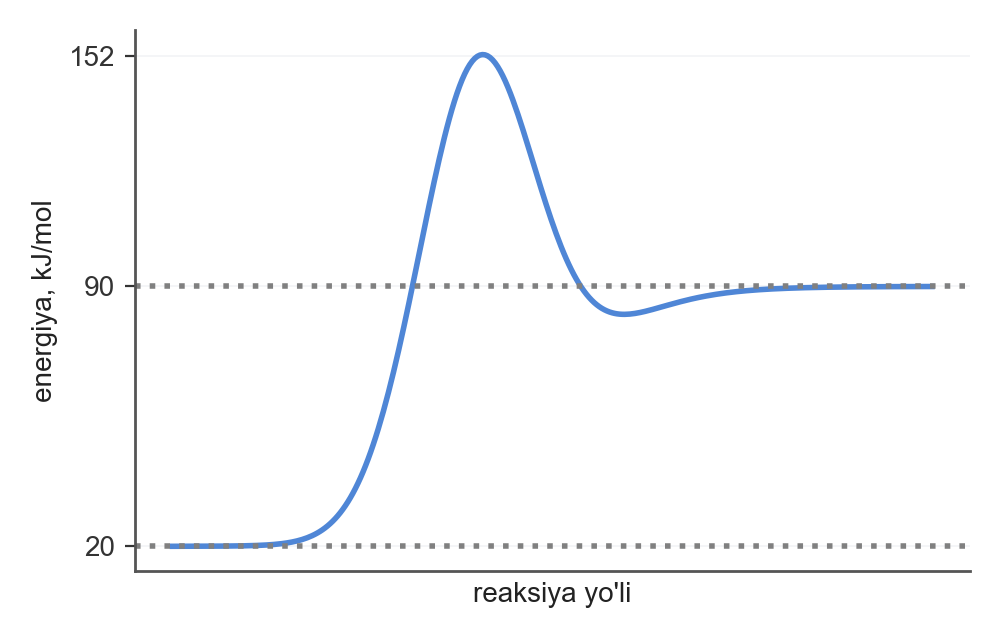
\includegraphics[width=0.86\linewidth]{rasmlar/gen/en_v05_0.png}\end{center}
To`g`ri reaksiyaning aktivlanish \textbf{energiyasini (kJ/mol) aniqlang.}

\noindent A)~\textsl{202} \hfill B)~\textsl{70} \hfill C)~\textsl{132} \hfill D)~\textsl{264}\par
\qsep
\noindent\qn{9.} Mn\textsubscript{2}O\textsubscript{7} tarkibida marganes ning \textbf{valentligini aniqlang.}

\noindent A)~\textsl{VII} \hfill B)~\textsl{II} \hfill C)~\textsl{\textit{V}} \hfill D)~\textsl{III}\par
\qsep
\noindent\qn{10.} Mis atomida d-pog`onachadagi elektronlar \textbf{sonini aniqlang} (\textit{Z} = 29).

\noindent A)~\textsl{11} \hfill B)~\textsl{9} \hfill C)~\textsl{12} \hfill D)~\textsl{10}\par
\qsep
\noindent\qn{11.} Cu + H\textsubscript{2}SO\textsubscript{4} $\to$ CuSO\textsubscript{4} + SO\textsubscript{2} + H\textsubscript{2}O reaksiyasida 2 mol Cu erisa, H\textsubscript{2}SO\textsubscript{4} ning necha moli oksidlovchi vazifasini bajaradi?

\noindent A)~\textsl{4} \hfill B)~\textsl{2} \hfill C)~\textsl{1} \hfill D)~\textsl{3}\par
\qsep
\noindent\qn{12.} HC$\equiv$C--CH=CH\textsubscript{2} molekulasida sp gibridlangan uglerod atomlari nechta?

\noindent A)~\textsl{3} \hfill B)~\textsl{4} \hfill C)~\textsl{1} \hfill D)~\textsl{2}\par
\qsep
\noindent\qn{13.} H\textsubscript{2} + I\textsubscript{2} $\rightleftarrows$ 2HI reaksiyada muvozanat holatida [H\textsubscript{2}] = 2, [I\textsubscript{2}] = 0,5, [HI] = 2 mol/l. Muvozanat \textbf{konstantasini (K) hisoblang.}

\noindent A)~\textsl{8} \hfill B)~\textsl{2} \hfill C)~\textsl{1,6} \hfill D)~\textsl{4}\par
\qsep
\noindent\qn{14.} Nodir gazlar haqida qaysi fikrlar to`g`ri? 1) Nodir gazlar kimyoviy jihatdan juda faol; 2) Geliy eng yengil inert gaz; 3) Argon havoning hajmi bo`yicha eng ko`p uchraydigan inert gazi; 4) Geliyda 8 ta tashqi elektron bor

\noindent A)~\textsl{3} \hfill B)~\textsl{2, 3} \hfill C)~\textsl{4} \hfill D)~\textsl{2, 3, 4}\par
\qsep
\noindent\qn{15.} 10,1 g KNO\textsubscript{3} to`liq parchalanguncha qizdirildi. Qattiq qoldiq \textbf{massasini (g) aniqlang.}

\noindent A)~\textsl{8,5} \hfill B)~\textsl{10,1} \hfill C)~\textsl{17} \hfill D)~\textsl{4,25}\par
\qsep
\noindent\qn{16.} Qaysi juftliklar o`zaro reaksiyaga kirishadi? 1) Ag va H\textsubscript{2}SO\textsubscript{4}(suyult.); 2) CO\textsubscript{2} va CaO; 3) Na\textsubscript{2}CO\textsubscript{3} va HCl; 4) Fe va HCl

\noindent A)~\textsl{3, 4} \hfill B)~\textsl{2, 3, 4} \hfill C)~\textsl{1, 3, 4} \hfill D)~\textsl{1, 3}\par
\qsep
\noindent\qn{17.} 44,8 l (n.sh.) ammiakdan nitrat kislota olindi (jami unum 80\%). Kislota \textbf{massasini (g) aniqlang.}

\noindent A)~\textsl{126} \hfill B)~\textsl{201,6} \hfill C)~\textsl{50,4} \hfill D)~\textsl{100,8}\par
\qsep
\noindent\qn{18.} 0,3 mol NaOH tutgan eritmadan 0,15 mol CO\textsubscript{2} o`tkazildi. Hosil bo`lgan Na\textsubscript{2}CO\textsubscript{3} \textbf{massasini (g) aniqlang.}

\noindent A)~\textsl{31,8} \hfill B)~\textsl{15,9} \hfill C)~\textsl{7,95} \hfill D)~\textsl{12}\par
\qsep
\noindent\qn{19.} 11,7 g NaCl ga mo`l kons. H\textsubscript{2}SO\textsubscript{4} ta'sir ettirilib, ajralgan HCl 500 g suvda eritildi. Hosil bo`lgan xlorid kislota massa \textbf{ulushini (\%) aniqlang.}

\noindent A)~\textsl{1,46} \hfill B)~\textsl{2,88} \hfill C)~\textsl{1,44} \hfill D)~\textsl{0,72}\par
\qsep
\noindent\qn{20.} Rasmda aromatik uglevodorod hosilasining tuzilish formulasi berilgan.
\begin{center}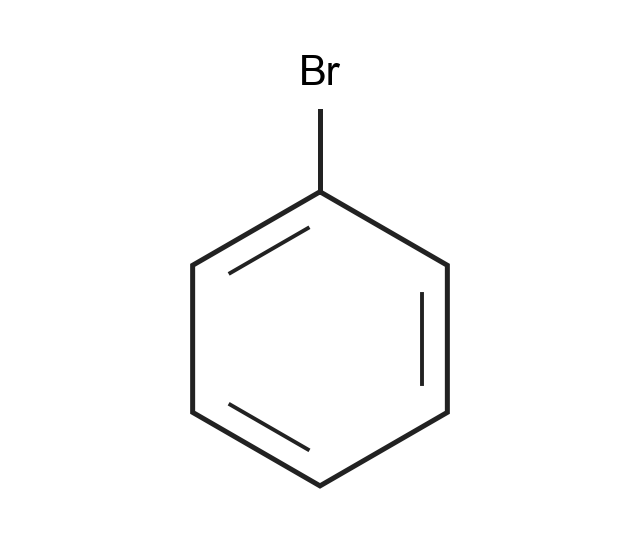
\includegraphics[width=0.86\linewidth]{rasmlar/gen/bz_539431.png}\end{center}
Birikmaning \textbf{nomini toping.}

\noindent\begin{tabular}{@{}p{0.47\linewidth}@{}p{0.47\linewidth}@{}}
A)~\textsl{toluol} & B)~\textsl{fenol} \\
C)~\textsl{brombenzol} & D)~\textsl{benzoy kislota} \\
\end{tabular}\par
\qsep
\noindent\qn{21.} Alken, alkadiyen va alkinlar haqida qaysi fikrlar to`g`ri? 1) Propenga HBr birikishi Markovnikov qoidasiga bo`ysunadi; 2) Alkinlar uchun umumiy formula CnH\textsubscript{2}n+2; 3) Asetilenni Kucherov reaksiyasi bilan sirka aldegidiga aylantirish mumkin; 4) Asetilen Ag\textsubscript{2}O ning ammiakli eritmasi bilan cho`kma beradi (butin-2 beradi)

\noindent A)~\textsl{1} \hfill B)~\textsl{1, 2} \hfill C)~\textsl{1, 3} \hfill D)~\textsl{3}\par
\qsep
\noindent\qn{22.} Arenlar, neft va tabiiy gaz haqida qaysi fikrlar to`g`ri? 1) Neft fraksiyalaridan gazolin 150 \textdegree{}C gacha haydaladi; 2) Naftalin -- bir halqali aren; 3) Benzoldan nitrobenzol nitrolash bilan olinadi; 4) Toluol KMnO\textsubscript{4} bilan benzoy kislotagacha oksidlanadi

\noindent A)~\textsl{2, 3} \hfill B)~\textsl{1, 2, 3} \hfill C)~\textsl{3, 4} \hfill D)~\textsl{1, 3, 4}\par
\qsep
\noindent\qn{23.} Reaksiya tenglamasi: C\textsubscript{6}H\textsubscript{12}O\textsubscript{6} $\to$ 2C\textsubscript{2}H\textsubscript{5}OH + 2CO\textsubscript{2}. Reaksiyaga 360 g C\textsubscript{6}H\textsubscript{12}O\textsubscript{6} kirishdi (unum 75\%). C\textsubscript{2}H\textsubscript{5}OH \textbf{massasini (g) hisoblang.}

\noindent A)~\textsl{46} \hfill B)~\textsl{138} \hfill C)~\textsl{276} \hfill D)~\textsl{69}\par
\qsep
\noindent\qn{24.} 2,3 g chumoli kislota Ag\textsubscript{2}O ning ammiakli eritmasi bilan to`liq oksidlanganda hosil bo`lgan kumush \textbf{massasini (g) aniqlang.}

\noindent A)~\textsl{10,8} \hfill B)~\textsl{5,4} \hfill C)~\textsl{21,6} \hfill D)~\textsl{2,3}\par
\qsep
\noindent\qn{25.} Karbon kislotalar haqida qaysi fikrlar to`g`ri? 1) Sirka angidrid ikki molekula sirka kislotadan suv chiqib hosil bo`ladi; 2) Olein kislota Br\textsubscript{2} ni biriktiradi; 3) Stearin kislota to`yinmagan kislota; 4) Sirka kislota karbonatlar bilan CO\textsubscript{2} ajratadi

\noindent A)~\textsl{1, 2, 4} \hfill B)~\textsl{1, 3, 4} \hfill C)~\textsl{3, 4} \hfill D)~\textsl{2, 3}\par
\qsep
\noindent\qn{26.} Murakkab efirlar va yog`lar haqida qaysi fikrlar to`g`ri? 1) Suyuq yog`larni gidrogenlab qattiq yog` olinadi; 2) Efirlanish reaksiyasi qaytmas; 3) Dietil efir spirtdan yuqori haroratda qaynaydi; 4) Sovun --- yuqori yog` kislotalarning natriyli tuzi

\noindent A)~\textsl{1, 4} \hfill B)~\textsl{2, 3} \hfill C)~\textsl{3, 4} \hfill D)~\textsl{4}\par
\qsep
\noindent\qn{27.} 6CO\textsubscript{2} + 6H\textsubscript{2}O $\to$ C\textsubscript{6}H\textsubscript{12}O\textsubscript{6} + 6O\textsubscript{2} jarayoni uchun 11,2 l (n.sh.) CO\textsubscript{2} olingan. O\textsubscript{2} \textbf{massasini (g) aniqlang.}

\noindent A)~\textsl{32} \hfill B)~\textsl{8} \hfill C)~\textsl{16} \hfill D)~\textsl{24}\par
\qsep
\noindent\qn{28.} Aminlar, aminokislotalar va oqsillar haqida qaysi fikrlar to`g`ri? 1) Nitrobenzoldan anilin Zinin reaksiyasi bilan olinadi; 2) Dipeptidda 2 ta peptid bog` bor; 3) Aminokislotalar amfoter birikmalar; 4) Anilin bromli suv bilan oq cho`kma beradi

\noindent A)~\textsl{1, 2} \hfill B)~\textsl{1, 3, 4} \hfill C)~\textsl{3, 4} \hfill D)~\textsl{1, 2, 4}\par
\qsep
\noindent\qn{29.} Yuqori molekulyar birikmalar haqida qaysi fikrlar to`g`ri? 1) Teflon --- polivinilxlorid; 2) Termoreaktiv polimerlar qizdirilganda qayta yumshaydi; 3) Lavsan poliamid tola; 4) Tabiiy kauchuk -- sis-1,4-poliizopren

\noindent A)~\textsl{1, 3} \hfill B)~\textsl{1} \hfill C)~\textsl{4} \hfill D)~\textsl{1, 4}\par
\qsep
\noindent\qn{30.} 100 g 10\% li Na\textsubscript{2}CO\textsubscript{3} eritmasini Na\textsubscript{2}CO\textsubscript{3}$\cdot$10H\textsubscript{2}O dan tayyorlash uchun necha gramm kristallogidrat kerak?

\noindent A)~\textsl{26,98} \hfill B)~\textsl{10} \hfill C)~\textsl{53,96} \hfill D)~\textsl{13,49}\par
\qsep
\noindent\qn{31.} Quyidagi aralashmani ajratish uchun qaysi usul mos: qum va suv aralashmasi?
\noindent A)~\textsl{filtrlash}\par
\noindent B)~\textsl{suvda eritib, filtrlash, so`ng bug`latish}\par
\noindent C)~\textsl{distillash (fraksiyalab haydash)}\par
\noindent D)~\textsl{ajratgich voronka}\par
\qsep
\noindent\qn{32.} Rasmdagi asbobda osh tuzining quruq kristallari lampochkani yondirmaydi, eritmasi esa yondiradi. Sababi nima?
\begin{center}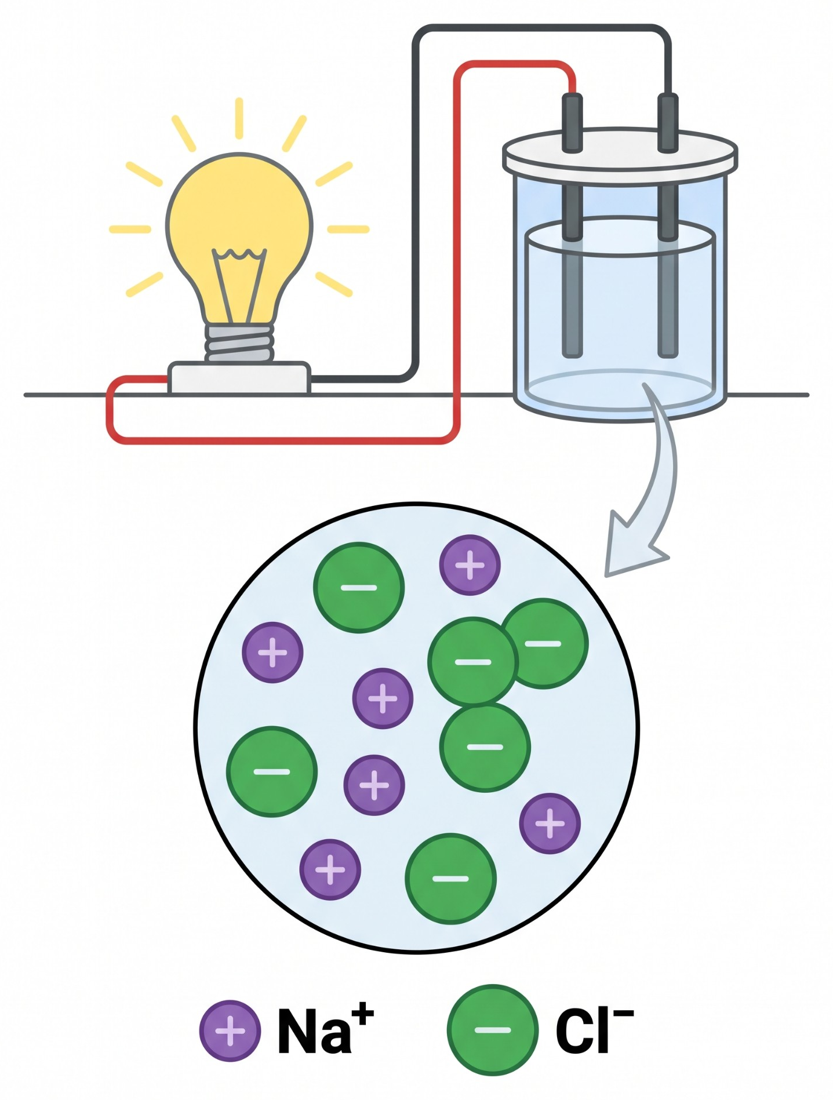
\includegraphics[width=0.86\linewidth]{rasmlar/darslik/d_elektr_asbob.png}\end{center}
\noindent A)~\textsl{eritmada erkin harakatlanuvchi ionlar hosil bo`ladi}\par
\noindent B)~\textsl{tuz suvda molekulalarga parchalanadi}\par
\noindent C)~\textsl{eritmada erkin elektronlar bor}\par
\noindent D)~\textsl{suv metall o`tkazgich   ---}\par
\qsep
\end{multicols}
\medskip
\noindent\setlength{\fboxsep}{0pt}\fbox{\begin{tabular}{p{0.74\linewidth}|p{0.2\linewidth}}
\parbox[t]{0.72\linewidth}{\vspace{3pt}\textbf{Topshiriqlar (33--35) va javob variant (A--F)larini o`zaro to`g`ri moslashtiring.} CaCO\textsubscript{3} va Na\textsubscript{2}CO\textsubscript{3} dan iborat 30,6 g aralashma mo`l xlorid kislota bilan reaksiyaga kirishdi. Ajralgan gaz 0,45 mol NaOH tutgan eritmadan o`tkazildi.
\vspace{3pt}} & \parbox[t]{0.19\linewidth}{\vspace{3pt}A~\textsl{13,44}\\[3pt]
B~\textsl{6,72}\\[3pt]
C~\textsl{10,08}\\[3pt]
D~\textsl{0,6}\\[3pt]
E~\textsl{5,38}\\[3pt]
F~\textsl{0,3}}\\ \hline
\parbox[t]{0.72\linewidth}{\vspace{2pt}\textbf{33. Ajralgan gazning hajmini (l, n.sh.) aniqlang.}\vspace{2pt}} & \\ \hline
\parbox[t]{0.72\linewidth}{\vspace{2pt}\textbf{34. Aralashmani to`liq eritish uchun sarflangan HCl miqdorini (mol) aniqlang.}\vspace{2pt}} & \\ \hline
\parbox[t]{0.72\linewidth}{\vspace{2pt}\textbf{35. Gaz NaOH eritmasidan o`tkazilganda hosil bo`lgan tuz (NaHCO\textsubscript{3}) massasini (g) aniqlang (reaksiya unumi 80\%).}\vspace{2pt}} & 
\end{tabular}}
\par\bigskip
\noindent\qn{36.} KMnO\textsubscript{4} + KI + H\textsubscript{2}SO\textsubscript{4} $\to$ MnSO\textsubscript{4} + I\textsubscript{2} + K\textsubscript{2}SO\textsubscript{4} + H\textsubscript{2}O reaksiya tenglamasini tenglang. Oksidlovchi va qaytaruvchi oldidagi koeffitsiyentlar \textbf{yig`indisini aniqlang.}
\javob\qsep
\noindent\qn{37.} H\textsubscript{2}SO\textsubscript{4} ning 0,025 mol/l li eritmasidan 0,4 l va Ba(OH)\textsubscript{2} ning 0,025 mol/l li eritmasidan 0,6 l aralashtirildi (umumiy hajm 1 l, ikkala modda to`liq dissotsilanadi, BaSO\textsubscript{4} cho`kmasi e'tiborga olinmasin). Hosil bo`lgan eritmaning pH \textbf{ini aniqlang.}
\javob\qsep
\noindent\qn{38.} NaBr va NaI dan iborat 28,1 g aralashma eritilib, mo`l xlor o`tkazildi, eritma bug`latilib quruq qoldiq 14,62 g chiqdi. Aralashmadagi NaI ning \textbf{massasini (g) toping.}
\javob\qsep
\noindent\qn{39.} Etilen va asetilendan iborat 4,48 l (n.sh.) aralashma bromli suvdan o`tkazilganda 40 g brom yutildi. Aralashmadagi asetilenning \textbf{hajmini (l, n.sh.) toping.}
\javob\qsep
\noindent\qn{40.} Alkanning vodorodga nisbatan zichligi 36, uglerodning massa ulushi 83,33\%. Shu alkan molekulasidagi $\sigma$-bog`lar umumiy \textbf{sonini toping.}
\javob\qsep
\par\bigskip\begin{center}\textbf{\fontsize{13}{15}\selectfont YOZMA ISH}\end{center}
\noindent\qn{41.} \textbf{Topshiriqni bajarish jarayonida barcha reaksiya tenglamalarini yozing. Miqdoriy va arifmetik hisoblashlarni (unga asos bo`lgan usul yoki formulani ko`rsatgan holda) uzviy ketma-ketlikda bajaring.}\par\smallskip
Tabiiy mis ikki izotopdan iborat: \textsuperscript{63}Cu (70\%) va \textsuperscript{65}Cu (30\%). 32 g shu element namunasi olingan (\textit{Z} = 29, N\textsubscript{A} = 6,02$\cdot$10\textsuperscript{23}).\par
\noindent 1)\ Elementning o`rtacha nisbiy atom massasini hisoblang.\par
\noindent 2)\ Namunadagi atomlarning umumiy miqdorini (mol) toping. Namunadagi protonlar sonini (mol) ham toping.\par
\noindent 3)\ Og`irroq izotop (\textsuperscript{65}Cu) atomlarining miqdorini (mol) hisoblang.\par
\noindent 4)\ Namunadagi neytronlarning umumiy miqdorini (mol) toping. Bitta atom massasini (g) ham hisoblang.\par
\noindent 5)\ Namunadagi atomlar sonini (10\textsuperscript{23} birligida) aniqlang. Namunadagi protonlar sonining neytronlar soniga nisbatini ham toping.\par
\diqqat{Mazkur topshiriq kengaytirilgan javobni talab etib, uning yechilish usuli va shu usul asosidagi barcha hisoblash amallari javoblar varaqasida aks etishi lozim.}\qsep
\noindent\qn{42.} Quyidagi o`zgarishlar zanjirida \textit{X}, \textit{Y}, \textit{Z} noma'lum organik moddalar:\par
\[\setlength{\fboxsep}{0pt}\text{C\textsubscript{2}H\textsubscript{5}Cl}\xrightarrow{\text{KOH (suvli)}}\text{\textit{X}}\xrightarrow{\text{H\textsubscript{2}SO\textsubscript{4} (kons.), 170 \textdegree{}C}}\text{\textit{Y}}\xrightarrow{\text{Br\textsubscript{2}}}\text{\textit{Z}}\xrightarrow{\text{KOH (spirtli)}}\text{C\textsubscript{2}H\textsubscript{2}}\]
\noindent 1)\ C\textsubscript{2}H\textsubscript{5}Cl $\to$ \textit{X} : reaksiya tenglamasini yozing; hosil bo`lgan moddani nomlang.\par
\noindent 2)\ \textit{X} $\to$ \textit{Y} : reaksiya tenglamasini yozing; hosil bo`lgan moddani nomlang.\par
\noindent 3)\ \textit{Y} $\to$ \textit{Z} : reaksiya tenglamasini yozing; hosil bo`lgan moddani nomlang.\par
\noindent 4)\ \textit{Z} $\to$ C\textsubscript{2}H\textsubscript{2} : reaksiya tenglamasini yozing; hosil bo`lgan moddani nomlang.\par
\diqqat{Mazkur topshiriq kengaytirilgan javobni talab etib, uning yechilish usuli va shu usul asosidagi barcha hisoblash amallari javoblar varaqasida aks etishi lozim.}\qsep
\noindent\qn{43.} \textbf{Topshiriqni bajarish jarayonida barcha reaksiya tenglamalarini yozing. Miqdoriy va arifmetik hisoblashlarni (unga asos bo`lgan usul yoki formulani ko`rsatgan holda) uzviy ketma-ketlikda bajaring.}\par\smallskip
CaCO\textsubscript{3} va MgCO\textsubscript{3} dan iborat 28,4 g aralashma doimiy massagacha qizdirildi. Ajralgan gaz mo`l Ca(OH)\textsubscript{2} eritmasidan o`tkazildi.\par
\noindent 1)\ Aralashmadagi har bir tuzning massasini (g) va massa ulushini (\%) aniqlang (reaksiya tenglamalarini yozing).\par
\noindent 2)\ Ajralgan gaz hajmini (l, n.sh.) va qattiq qoldiq massasini (g) toping. Qoldiqdagi CaO ning massa ulushini (\%) ham hisoblang.\par
\noindent 3)\ Gaz Ca(OH)\textsubscript{2} eritmasidan o`tkazilganda hosil bo`lgan cho`kma massasini (g) hisoblang.\par
\noindent 4)\ Qattiq qoldiqni to`liq eritish uchun 10\% li HCl eritmasidan necha gramm kerak?\par
\noindent 5)\ Qoldiq oksidlar suvga solinganda hosil bo`ladigan Ca(OH)\textsubscript{2} massasini (g) toping (CaO + H\textsubscript{2}O $\to$ Ca(OH)\textsubscript{2}).\par
\diqqat{Mazkur topshiriq kengaytirilgan javobni talab etib, uning yechilish usuli va shu usul asosidagi barcha hisoblash amallari javoblar varaqasida aks etishi lozim.}\qsep
\newpage
\renewcommand{\curvar}{6-variant}
\thispagestyle{first}
\noindent\textit{Davriy jadvaldan foydalanish mumkin.}
\par\smallskip
\begin{multicols}{2}
\noindent\qn{1.} Rasmda kristall panjara tuzilishi tasvirlangan.
\begin{center}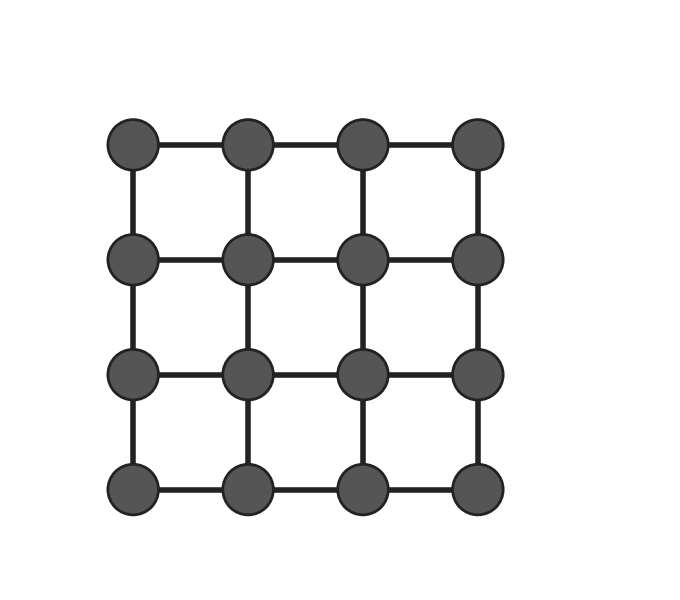
\includegraphics[width=0.86\linewidth]{rasmlar/gen/la_142898.png}\end{center}
Shunday panjarali moddalar uchun qaysi xususiyat xos?
\noindent A)~\textsl{Yuqori suyuqlanish harorati, suyuqlanmasi elektr tokini o`tkazadi}\par
\noindent B)~\textsl{Past suyuqlanish harorati, uchuvchan}\par
\noindent C)~\textsl{Juda qattiq, suyuqlanish harorati juda yuqori}\par
\noindent D)~\textsl{Elektr tokini yaxshi o`tkazadi, plastik}\par
\qsep
\noindent\qn{2.} 4 g metall oksidlanganda 5,6 g oksid hosil bo`ldi. Metallning ekvivalent \textbf{massasini (g/mol) aniqlang.}

\noindent A)~\textsl{40} \hfill B)~\textsl{20} \hfill C)~\textsl{10} \hfill D)~\textsl{30}\par
\qsep
\noindent\qn{3.} Radioaktiv izotop yadrolari sonining vaqtga bog`liqligi grafikda berilgan.
\begin{center}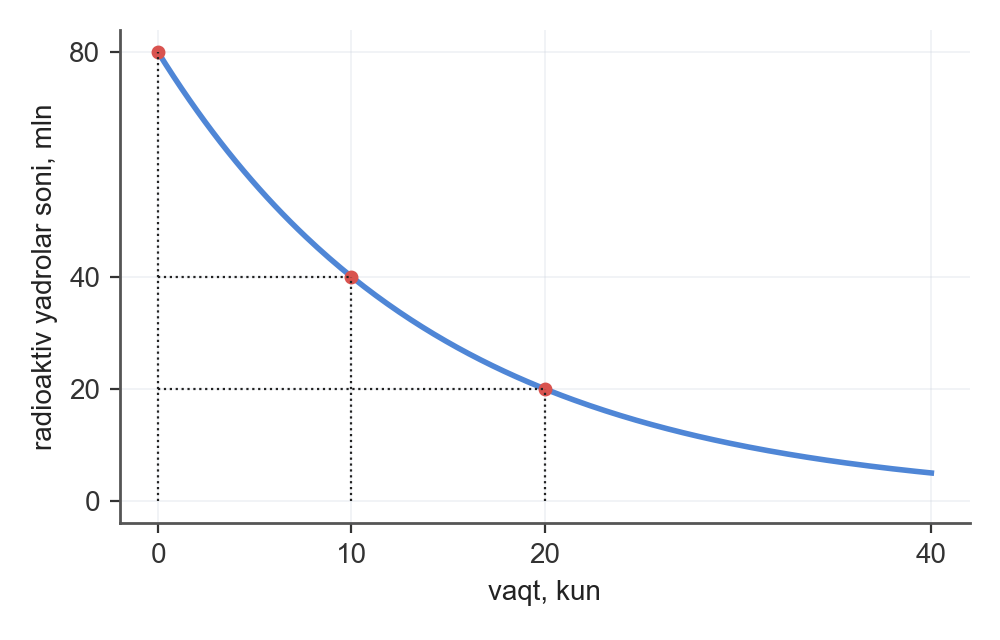
\includegraphics[width=0.86\linewidth]{rasmlar/gen/de_v06_0.png}\end{center}
20 kundan keyin necha mln yadro yemirilgan bo`ladi?

\noindent A)~\textsl{20} \hfill B)~\textsl{60} \hfill C)~\textsl{40} \hfill D)~\textsl{80}\par
\qsep
\noindent\qn{4.} C\textsubscript{6}H\textsubscript{5}CH\textsubscript{3} molekulasidagi $\sigma$ va $\pi$ bog`lar \textbf{sonini aniqlang.}

\noindent A)~\textsl{15 va 3} \hfill B)~\textsl{14 va 3} \hfill C)~\textsl{15 va 4} \hfill D)~\textsl{16 va 3}\par
\qsep
\noindent\qn{5.} Jadvalda Mn elementining birikmalaridagi oksidlanish darajasi berilgan:
\begin{center}
\renewcommand{\arraystretch}{1.15}
\fitbox{\begin{tabular}{|c|c|}\hline
\textbf{Modda} & \textbf{Oksidlanish darajasi} \\ \hline
K\textsubscript{2}MnO\textsubscript{4} & +6 \\ \hline
MnO\textsubscript{2} & +4 \\ \hline
KMnO\textsubscript{4} & +7 \\ \hline
MnSO\textsubscript{4} & +2 \\ \hline
\end{tabular}}
\end{center}
Ushbu moddalardan nechtasida Mn elementi ham oksidlovchi, ham qaytaruvchi xossani namoyon qiladi? (Mn uchun eng past oksidlanish darajasi 0, eng yuqorisi +7)

\noindent A)~\textsl{3} \hfill B)~\textsl{4} \hfill C)~\textsl{5} \hfill D)~\textsl{1}\par
\qsep
\noindent\qn{6.} Gazlar aralashmasi tarkibi jadvalda berilgan (n.sh.):
\begin{center}
\renewcommand{\arraystretch}{1.15}
\fitbox{\begin{tabular}{|c|c|}\hline
\textbf{Gaz} & \textbf{Hajmi, l} \\ \hline
H\textsubscript{2} & 3 \\ \hline
NH\textsubscript{3} & 2 \\ \hline
CH\textsubscript{4} & 3 \\ \hline
\end{tabular}}
\end{center}
Aralashmaning havoga nisbatan \textbf{zichligini aniqlang} (M(havo) = 29 g/mol).

\noindent A)~\textsl{0,76} \hfill B)~\textsl{0,19} \hfill C)~\textsl{0,38} \hfill D)~\textsl{11}\par
\qsep
\noindent\qn{7.} K\textsubscript{2}CO\textsubscript{3} ning suvli eritmasi inert elektrodlar bilan elektroliz qilinganda qaysi moddalar ajraladi?

\noindent\begin{tabular}{@{}p{0.47\linewidth}@{}p{0.47\linewidth}@{}}
A)~\textsl{Zn, H\textsubscript{2} va O\textsubscript{2}} & B)~\textsl{H\textsubscript{2} va O\textsubscript{2}} \\
C)~\textsl{Cu va Cl\textsubscript{2}} & D)~\textsl{Ag va O\textsubscript{2}} \\
\end{tabular}\par
\qsep
\noindent\qn{8.} S + HNO\textsubscript{3} $\to$ H\textsubscript{2}SO\textsubscript{4} + NO reaksiya tenglamasini tenglang va barcha koeffitsiyentlar \textbf{yig`indisini aniqlang.}

\noindent A)~\textsl{7} \hfill B)~\textsl{5} \hfill C)~\textsl{8} \hfill D)~\textsl{6}\par
\qsep
\noindent\qn{9.} Zn plastinka 33,1 g Pb(NO\textsubscript{3})\textsubscript{2} ni tutgan eritmaga tushirildi va Pb to`liq ajralib chiqquncha ushlab turildi. Plastinka massasi necha gramm ortadi?

\noindent A)~\textsl{28,4} \hfill B)~\textsl{7,1} \hfill C)~\textsl{33,1} \hfill D)~\textsl{14,2}\par
\qsep
\noindent\qn{10.} Massasi 7 g bo`lgan gaz 27 \textdegree{}C va 0,5 atm bosimda 12,3 l hajm egallaydi. Gazning vodorodga nisbatan \textbf{zichligini aniqlang.} (R = 0,082 l$\cdot$atm/(mol$\cdot$K))

\noindent A)~\textsl{14} \hfill B)~\textsl{28} \hfill C)~\textsl{7} \hfill D)~\textsl{56}\par
\qsep
\noindent\qn{11.} Quyidagi zarrachalardan qaysilari argon atomi bilan izoelektron? 1) Ca\textsuperscript{2+}; 2) K\textsuperscript{+}; 3) Cl\textsuperscript{$-$}; 4) Li\textsuperscript{+}

\noindent A)~\textsl{1, 2} \hfill B)~\textsl{1, 2, 3} \hfill C)~\textsl{1, 2, 4} \hfill D)~\textsl{1, 3}\par
\qsep
\noindent\qn{12.} 30-tartib raqamli element atomida n = 3 va l = 2 bo`lgan elektronlar \textbf{sonini aniqlang.}

\noindent A)~\textsl{11} \hfill B)~\textsl{10} \hfill C)~\textsl{9} \hfill D)~\textsl{12}\par
\qsep
\noindent\qn{13.} \textit{X} moddaning parchalanish reaksiyasida konsentratsiyaning vaqt bo`yicha o`zgarishi jadvalda berilgan:
\begin{center}
\renewcommand{\arraystretch}{1.15}
\fitbox{\begin{tabular}{|c|c|}\hline
\textbf{t, min} & \textbf{c, mol/l} \\ \hline
0 & 2,4 \\ \hline
2 & 1,92 \\ \hline
4 & 1,44 \\ \hline
6 & 0,96 \\ \hline
\end{tabular}}
\end{center}
0-minutdan 2-minutgacha o`rtacha tezlikni mol/(l$\cdot$min) \textbf{hisoblang.}

\noindent A)~\textsl{0,48} \hfill B)~\textsl{0,12} \hfill C)~\textsl{1,2} \hfill D)~\textsl{0,24}\par
\qsep
\noindent\qn{14.} Qaysi juftliklar o`zaro reaksiyaga kirishadi? 1) SiO\textsubscript{2} va H\textsubscript{2}O; 2) Ag va H\textsubscript{2}SO\textsubscript{4}(suyult.); 3) MgCl\textsubscript{2} va KNO\textsubscript{3}; 4) Fe va HCl

\noindent A)~\textsl{2, 3} \hfill B)~\textsl{1} \hfill C)~\textsl{3, 4} \hfill D)~\textsl{4}\par
\qsep
\noindent\qn{15.} 37,8 g Zn(NO\textsubscript{3})\textsubscript{2} to`liq parchalanguncha qizdirildi. Qattiq qoldiq \textbf{massasini (g) aniqlang.}

\noindent A)~\textsl{16,2} \hfill B)~\textsl{37,8} \hfill C)~\textsl{32,4} \hfill D)~\textsl{8,1}\par
\qsep
\noindent\qn{16.} 0,2 mol NaOH tutgan eritmadan 0,15 mol CO\textsubscript{2} o`tkazildi. Hosil bo`lgan NaHCO\textsubscript{3} \textbf{massasini (g) aniqlang.}

\noindent A)~\textsl{8,4} \hfill B)~\textsl{4,2} \hfill C)~\textsl{2,1} \hfill D)~\textsl{8}\par
\qsep
\noindent\qn{17.} Reaksiya tenglamasi: 2NaCl + H\textsubscript{2}SO\textsubscript{4} $\to$ Na\textsubscript{2}SO\textsubscript{4} + 2HCl. Reaksiyaga 196 g H\textsubscript{2}SO\textsubscript{4} kirishdi. HCl \textbf{massasini (g) hisoblang.}

\noindent A)~\textsl{36,5} \hfill B)~\textsl{292} \hfill C)~\textsl{146} \hfill D)~\textsl{73}\par
\qsep
\noindent\qn{18.} Li va K dan iborat 6 g aralashma suv bilan reaksiyaga kirishdi. Ajralgan vodorodning \textbf{hajmini (l, n.sh.) aniqlang.}

\noindent A)~\textsl{4,48} \hfill B)~\textsl{8,96} \hfill C)~\textsl{2,24} \hfill D)~\textsl{3}\par
\qsep
\noindent\qn{19.} Alyuminiy (0,2 mol) va magniy (0,2 mol) aralashmasi mo`l xlorid kislotada eritildi. Ajralgan vodorodning \textbf{hajmini (l, n.sh.) aniqlang.}

\noindent A)~\textsl{11,2} \hfill B)~\textsl{8,96} \hfill C)~\textsl{22,4} \hfill D)~\textsl{5,6}\par
\qsep
\noindent\qn{20.} CH\textsubscript{3}--CH(CH\textsubscript{3})--CH(C\textsubscript{2}H\textsubscript{5})--CH\textsubscript{2}--CH\textsubscript{3} birikmaning sistematik nomi qaysi qatorda to`g`ri keltirilgan?

\noindent\begin{tabular}{@{}p{0.47\linewidth}@{}p{0.47\linewidth}@{}}
A)~\textsl{2-metil-3-etilpentan} & B)~\textsl{3-izopropilpentan} \\
C)~\textsl{3-etil-2-metilpentan} & D)~\textsl{2,3-dietilbutan} \\
\end{tabular}\par
\qsep
\noindent\qn{21.} Alken, alkadiyen va alkinlar haqida qaysi fikrlar to`g`ri? 1) Asetilen Ag\textsubscript{2}O ning ammiakli eritmasi bilan cho`kma beradi (butin-2 beradi); 2) Etilen sanoatda kreking gazlaridan olinadi; 3) Alkinlar uchun umumiy formula CnH\textsubscript{2}n+2; 4) Kauchuk izoprenning polimeri

\noindent A)~\textsl{1, 3} \hfill B)~\textsl{1, 4} \hfill C)~\textsl{2, 4} \hfill D)~\textsl{1, 3, 4}\par
\qsep
\noindent\qn{22.} 18,8 g fenoldan 2,4,6-tribromfenol olishda unum 75\% bo`lsa, mahsulot \textbf{massasini (g) aniqlang.}

\noindent A)~\textsl{66,2} \hfill B)~\textsl{99,3} \hfill C)~\textsl{14,1} \hfill D)~\textsl{49,65}\par
\qsep
\noindent\qn{23.} C\textsubscript{6}H\textsubscript{5}OH + 3Br\textsubscript{2} $\to$ C\textsubscript{6}H\textsubscript{2}Br\textsubscript{3}OH + 3HBr reaksiyasida 9,4 g C\textsubscript{6}H\textsubscript{5}OH ishtirok etdi. C\textsubscript{6}H\textsubscript{2}Br\textsubscript{3}OH \textbf{miqdorini (mol) toping.}

\noindent A)~\textsl{0,1} \hfill B)~\textsl{0,2} \hfill C)~\textsl{0,05} \hfill D)~\textsl{0,15}\par
\qsep
\noindent\qn{24.} 11,6 g propanal Ag\textsubscript{2}O ning ammiakli eritmasi bilan to`liq oksidlanganda hosil bo`lgan kumush \textbf{massasini (g) aniqlang.}

\noindent A)~\textsl{21,6} \hfill B)~\textsl{43,2} \hfill C)~\textsl{86,4} \hfill D)~\textsl{11,6}\par
\qsep
\noindent\qn{25.} 60 g CH\textsubscript{3}COOH dan quyidagi ikki bosqichda Na\textsubscript{2}CO\textsubscript{3} olinadi: 1) CH\textsubscript{3}COOH + NaOH $\to$ CH\textsubscript{3}COONa + H\textsubscript{2}O (unum 90\%); 2) CH\textsubscript{3}COONa + NaOH $\to$ CH\textsubscript{4} + Na\textsubscript{2}CO\textsubscript{3} (unum 50\%). Oxirgi mahsulot Na\textsubscript{2}CO\textsubscript{3} ning \textbf{massasini (g) toping.}

\noindent A)~\textsl{53} \hfill B)~\textsl{95,4} \hfill C)~\textsl{47,7} \hfill D)~\textsl{106}\par
\qsep
\noindent\qn{26.} 60 g CH\textsubscript{3}COOH dan quyidagi ikki bosqichda CH\textsubscript{3}COONa olinadi: 1) CH\textsubscript{3}COOH + C\textsubscript{2}H\textsubscript{5}OH $\to$ CH\textsubscript{3}COOC\textsubscript{2}H\textsubscript{5} + H\textsubscript{2}O (unum 60\%); 2) CH\textsubscript{3}COOC\textsubscript{2}H\textsubscript{5} + NaOH $\to$ CH\textsubscript{3}COONa + C\textsubscript{2}H\textsubscript{5}OH (unum 50\%). Oxirgi mahsulot CH\textsubscript{3}COONa ning \textbf{massasini (g) toping.}

\noindent A)~\textsl{41} \hfill B)~\textsl{24,6} \hfill C)~\textsl{49,2} \hfill D)~\textsl{82}\par
\qsep
\noindent\qn{27.} Uglevodlar haqida qaysi fikrlar to`g`ri? 1) Kraxmal va selluloza bir xil M ga ega; 2) Saxaroza Feling suyuqligini qaytaradi; 3) Maltoza gidrolizlanganda ikki molekula glyukoza hosil qiladi; 4) Glyukoza "kumush ko`zgu" reaksiyasini beradi

\noindent A)~\textsl{3, 4} \hfill B)~\textsl{1, 3} \hfill C)~\textsl{2} \hfill D)~\textsl{2, 3}\par
\qsep
\noindent\qn{28.} Quyidagi birikmalardan qaysi biri fenol sinfiga kiradi?

\noindent\begin{tabular}{@{}p{0.47\linewidth}@{}p{0.47\linewidth}@{}}
A)~\textsl{H\textsubscript{2}NCH\textsubscript{2}COOH} & B)~\textsl{CH\textsubscript{3}CHO} \\
C)~\textsl{C\textsubscript{6}H\textsubscript{12}O\textsubscript{6}} & D)~\textsl{C\textsubscript{6}H\textsubscript{5}OH} \\
\end{tabular}\par
\qsep
\noindent\qn{29.} Izobutilen monomeridan olingan polimerning molyar massasi 140000 g/mol. Polimerlanish \textbf{darajasini aniqlang.}

\noindent A)~\textsl{5000} \hfill B)~\textsl{1250} \hfill C)~\textsl{2500} \hfill D)~\textsl{2510}\par
\qsep
\noindent\qn{30.} Rasmdagi tajribada etanolga konsentrlangan H\textsubscript{2}SO\textsubscript{4} ning vazifasi nima?
\begin{center}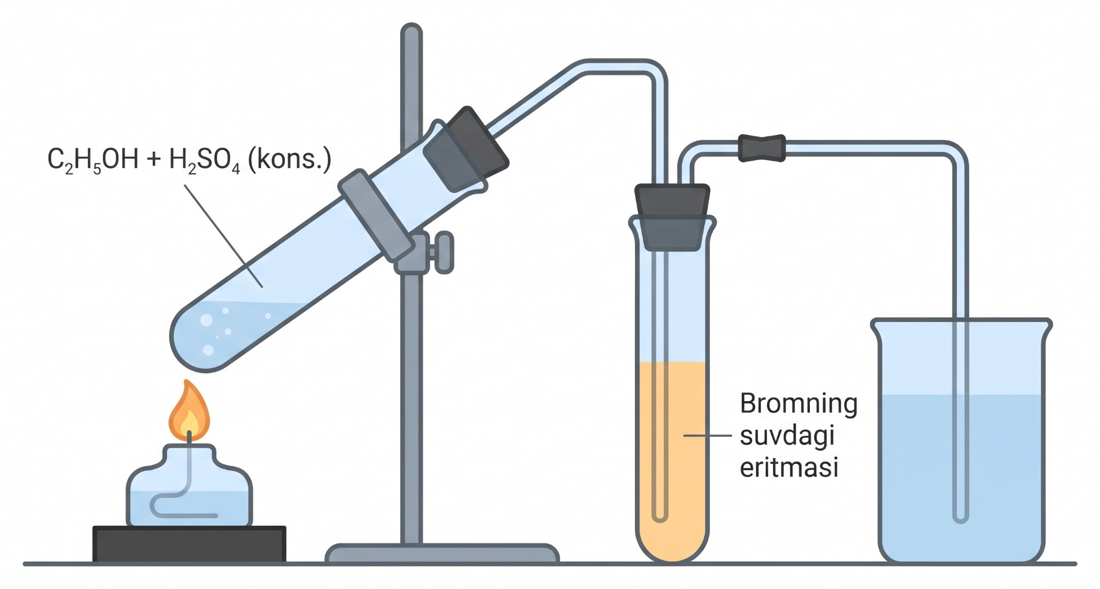
\includegraphics[width=0.86\linewidth]{rasmlar/darslik/d_etilen.png}\end{center}
\noindent A)~\textsl{oksidlovchi, etilenni oksidlaydi}\par
\noindent B)~\textsl{faqat erituvchi}\par
\noindent C)~\textsl{reaksiyada ishtirok etmaydi}\par
\noindent D)~\textsl{suv tortuvchi va katalizator}\par
\qsep
\noindent\qn{31.} Kimyo laboratoriyasida ishlash qoidalari haqida qaysi fikrlar to`g`ri? 1) Zaharli gaz ajraladigan tajriba mo`rili shkafda o`tkaziladi; 2) Kimyoviy moddalar hidini bevosita nafas olib aniqlash kerak; 3) Suvni konsentrlangan kislotaga tez quyish mumkin; 4) Ortiqcha reaktiv idishga qaytariladi

\noindent A)~\textsl{1, 4} \hfill B)~\textsl{1, 3} \hfill C)~\textsl{1} \hfill D)~\textsl{4}\par
\qsep
\noindent\qn{32.} 400 g 4\% li CuSO\textsubscript{4} eritmasini CuSO\textsubscript{4}$\cdot$5H\textsubscript{2}O dan tayyorlash uchun necha gramm kristallogidrat kerak?

\noindent A)~\textsl{16} \hfill B)~\textsl{50} \hfill C)~\textsl{12,5} \hfill D)~\textsl{25   ---}\par
\qsep
\end{multicols}
\medskip
\noindent\setlength{\fboxsep}{0pt}\fbox{\begin{tabular}{p{0.74\linewidth}|p{0.2\linewidth}}
\parbox[t]{0.72\linewidth}{\vspace{3pt}\textbf{Topshiriqlar (33--35) va javob variant (A--F)larini o`zaro to`g`ri moslashtiring.} CuO va Fe\textsubscript{2}O\textsubscript{3} dan iborat 32 g aralashma qizdirilib, H\textsubscript{2} oqimida to`liq qaytarildi; qoldiq (metallar) massasi 24 g.
\vspace{3pt}} & \parbox[t]{0.19\linewidth}{\vspace{3pt}A~\textsl{18}\\[3pt]
B~\textsl{9}\\[3pt]
C~\textsl{16}\\[3pt]
D~\textsl{13,44}\\[3pt]
E~\textsl{12,8}\\[3pt]
F~\textsl{24}}\\ \hline
\parbox[t]{0.72\linewidth}{\vspace{2pt}\textbf{33. Aralashmadagi CuO massasini (g) aniqlang.}\vspace{2pt}} & \\ \hline
\parbox[t]{0.72\linewidth}{\vspace{2pt}\textbf{34. Qaytarish uchun (20\% ortiqcha olingan) sarflangan H\textsubscript{2} hajmini (l, n.sh.) aniqlang.}\vspace{2pt}} & \\ \hline
\parbox[t]{0.72\linewidth}{\vspace{2pt}\textbf{35. Qaytarish natijasida hosil bo`lgan suv massasini (g) aniqlang.}\vspace{2pt}} & 
\end{tabular}}
\par\bigskip
\noindent\qn{36.} KMnO\textsubscript{4} + Na\textsubscript{2}SO\textsubscript{3} + H\textsubscript{2}O $\to$ MnO\textsubscript{2} + Na\textsubscript{2}SO\textsubscript{4} + KOH reaksiya tenglamasini tenglang. Reagentlar (chap qism) koeffitsiyentlari \textbf{yig`indisini toping.}
\javob\qsep
\noindent\qn{37.} NaCl eritmasi inert elektrodlar yordamida 2 A tok kuchi bilan 3860 s elektroliz qilindi. Katodda ajralgan H\textsubscript{2} massasi (g) \textbf{ni toping.}
\javob\qsep
\noindent\qn{38.} Zn va ZnO dan iborat 22,7 g aralashma mo`l NaOH eritmasida eritilganda 2,24 l (n.sh.) vodorod ajraldi. Aralashmadagi ZnO \textbf{massasini (g) aniqlang.}
\javob\qsep
\noindent\qn{39.} Etanol va fenoldan iborat 23,4 g aralashma natriy bilan to`liq reaksiyaga kirishganda 3,36 l (n.sh.) vodorod ajraldi. Shu aralashmaga mo`l bromli suv ta'sir ettirilganda hosil bo`ladigan cho`kma \textbf{massasini (g) toping.}
\javob\qsep
\noindent\qn{40.} Etilen monomeridan olingan polimerning molyar massasi 56000 g/mol. Polimerlanish \textbf{darajasini aniqlang.}
\javob\qsep
\par\bigskip\begin{center}\textbf{\fontsize{13}{15}\selectfont YOZMA ISH}\end{center}
\noindent\qn{41.} \textbf{Topshiriqni bajarish jarayonida barcha reaksiya tenglamalarini yozing. Miqdoriy va arifmetik hisoblashlarni (unga asos bo`lgan usul yoki formulani ko`rsatgan holda) uzviy ketma-ketlikda bajaring.}\par\smallskip
300 g 20\% li NaCl eritmasi inert elektrodlar yordamida 5 A tok kuchi bilan 3860 s elektroliz qilindi.\par
\noindent 1)\ Katodda va anodda ajralgan gazlarning hajmlarini (l, n.sh.) hisoblang.\par
\noindent 2)\ Elektrolizdan keyingi eritma massasini (g) aniqlang. Ajralgan gazlarning umumiy massasini (g) ham hisoblang.\par
\noindent 3)\ Elektrolizdan keyingi eritmada NaOH ning massa ulushini (\%) toping.\par
\noindent 4)\ Hosil bo`lgan NaOH ni to`liq neytrallash uchun 10\% li HCl eritmasidan necha gramm kerak? Hosil bo`lgan NaCl massasini (g) ham hisoblang.\par
\noindent 5)\ Anodda ajralgan xlor KI eritmasidan o`tkazilsa, ajralgan yod massasini (g) aniqlang. Anodda ajralgan xlorning massasini (g) ham toping.\par
\diqqat{Mazkur topshiriq kengaytirilgan javobni talab etib, uning yechilish usuli va shu usul asosidagi barcha hisoblash amallari javoblar varaqasida aks etishi lozim.}\qsep
\noindent\qn{42.} Reaksiya tenglamalarini tugallang va tenglang. Hosil bo`lgan organik moddalarning tuzilish formulalarini yozing va ularni nomlang.\par
\noindent 1)\ C\textsubscript{6}H\textsubscript{5}--CH\textsubscript{3} + Cl\textsubscript{2} $\xrightarrow{\text{yorug`lik}}$\par
\noindent 2)\ CH\textsubscript{3}--CH\textsubscript{2}--OH + CuO $\xrightarrow{\text{t}}$\par
\noindent 3)\ 2CH\textsubscript{4} $\xrightarrow{\text{1500 \textdegree{}C}}$\par
\noindent 4)\ CH\textsubscript{3}CHO + Ag\textsubscript{2}O $\xrightarrow{\text{NH\textsubscript{3}, t}}$\par
\noindent 5)\ C\textsubscript{2}H\textsubscript{5}Br + KOH(spirtli) $\to$\par
\noindent 6)\ n CH\textsubscript{2}=CH--CH=CH\textsubscript{2} $\to$\par
\noindent 7)\ CH\textsubscript{3}--CH=CH\textsubscript{2} + HBr $\to$\par
\diqqat{Mazkur topshiriq kengaytirilgan javobni talab etib, uning yechilish usuli va shu usul asosidagi barcha hisoblash amallari javoblar varaqasida aks etishi lozim.}\qsep
\noindent\qn{43.} \textbf{Topshiriqni bajarish jarayonida barcha reaksiya tenglamalarini yozing. Miqdoriy va arifmetik hisoblashlarni (unga asos bo`lgan usul yoki formulani ko`rsatgan holda) uzviy ketma-ketlikda bajaring.}\par\smallskip
0,05 mol AlCl\textsubscript{3} saqlagan eritmaga NaOH eritmasi qo`shildi. Avval 0,15 mol NaOH qo`shilganda cho`kma hosil bo`ldi, so`ng yana 0,05 mol NaOH qo`shilganda cho`kma to`liq erib ketdi (Na[Al(OH)\textsubscript{4}] hosil bo`ldi).\par
\noindent 1)\ Cho`kma hosil bo`lish va erish reaksiyalari tenglamalarini yozing. Cho`kma massasini (g) hisoblang.\par
\noindent 2)\ Jami sarflangan NaOH massasini (g) aniqlang.\par
\noindent 3)\ Hosil bo`lgan Na[Al(OH)\textsubscript{4}] eritmasidan mo`l CO\textsubscript{2} o`tkazilganda cho`kadigan Al(OH)\textsubscript{3} massasini (g) toping.\par
\noindent 4)\ Al(OH)\textsubscript{3} cho`kmasi qizdirilganda hosil bo`ladigan oksid massasini (g) hisoblang.\par
\noindent 5)\ Na[Al(OH)\textsubscript{4}] eritmasining hajmi 500 ml bo`lsa, tuzning molyar konsentratsiyasini (mol/l) hisoblang.\par
\diqqat{Mazkur topshiriq kengaytirilgan javobni talab etib, uning yechilish usuli va shu usul asosidagi barcha hisoblash amallari javoblar varaqasida aks etishi lozim.}\qsep
\newpage
\renewcommand{\curvar}{7-variant}
\thispagestyle{first}
\noindent\textit{Davriy jadvaldan foydalanish mumkin.}
\par\smallskip
\begin{multicols}{2}
\noindent\qn{1.} 1 mol CO\textsubscript{2} tarkibida necha mol atom bor?

\noindent A)~\textsl{3} \hfill B)~\textsl{2} \hfill C)~\textsl{4} \hfill D)~\textsl{1}\par
\qsep
\noindent\qn{2.} pH = 9 bo`lgan eritmada gidroksid ionlari konsentratsiyasi 10\textsuperscript{$-$x} mol/l ga teng. x \textbf{ni aniqlang.}

\noindent A)~\textsl{9} \hfill B)~\textsl{5} \hfill C)~\textsl{6} \hfill D)~\textsl{8}\par
\qsep
\noindent\qn{3.} Tuzning eruvchanligi yuqori haroratda 150 g, past haroratda 40 g (100 g suvda). Yuqori haroratda to`yingan 500 g eritma past haroratgacha sovitilsa, necha gramm tuz cho`kmaga tushadi?

\noindent A)~\textsl{300} \hfill B)~\textsl{80} \hfill C)~\textsl{220} \hfill D)~\textsl{440}\par
\qsep
\noindent\qn{4.} Zichligi 1,11 g/ml bo`lgan 10\% li NaOH eritmasining molyar \textbf{konsentratsiyasini (mol/l) aniqlang.}

\noindent A)~\textsl{2,78} \hfill B)~\textsl{0,28} \hfill C)~\textsl{5,55} \hfill D)~\textsl{2,5}\par
\qsep
\noindent\qn{5.} Gazlar aralashmasi tarkibi jadvalda berilgan (n.sh.):
\begin{center}
\renewcommand{\arraystretch}{1.15}
\fitbox{\begin{tabular}{|c|c|}\hline
\textbf{Gaz} & \textbf{Hajmi, l} \\ \hline
CO\textsubscript{2} & 1 \\ \hline
N\textsubscript{2} & 2 \\ \hline
SO\textsubscript{2} & 3 \\ \hline
\end{tabular}}
\end{center}
Aralashmaning havoga nisbatan \textbf{zichligini aniqlang} (M(havo) = 29 g/mol).

\noindent A)~\textsl{1,68} \hfill B)~\textsl{3,36} \hfill C)~\textsl{0,84} \hfill D)~\textsl{48,67}\par
\qsep
\noindent\qn{6.} Metall oksidida kislorodning massa ulushi 22,22\%. Metallning ekvivalent \textbf{massasini (g/mol) aniqlang.}

\noindent A)~\textsl{56} \hfill B)~\textsl{14} \hfill C)~\textsl{28} \hfill D)~\textsl{42}\par
\qsep
\noindent\qn{7.} Jadvalda nuklidlarning proton soni (\textit{Z}) va massa soni (A) berilgan:
\begin{center}
\renewcommand{\arraystretch}{1.15}
\fitbox{\begin{tabular}{|c|c|c|}\hline
\textbf{Nuklid} & \textbf{\textit{Z}} & \textbf{A} \\ \hline
\textit{X} & 20 & 40 \\ \hline
\textit{Y} & 20 & 42 \\ \hline
T & 21 & 40 \\ \hline
\textit{U} & 21 & 41 \\ \hline
\textit{V} & 20 & 42 \\ \hline
\end{tabular}}
\end{center}
\textit{X} nuklidning nechta izobari jadvalda keltirilgan?

\noindent A)~\textsl{2} \hfill B)~\textsl{3} \hfill C)~\textsl{1} \hfill D)~\textsl{4}\par
\qsep
\noindent\qn{8.} Quyidagi tuzlarning qaysilari suvli eritmasi ishqoriy muhitga ega? 1) CH\textsubscript{3}COONa; 2) FeCl\textsubscript{3}; 3) Al\textsubscript{2}(SO\textsubscript{4})\textsubscript{3}; 4) Na\textsubscript{2}CO\textsubscript{3}

\noindent A)~\textsl{1, 3} \hfill B)~\textsl{3} \hfill C)~\textsl{1} \hfill D)~\textsl{1, 4}\par
\qsep
\noindent\qn{9.} Hajmi 5 l bo`lgan idishda A modda miqdori 30 s davomida 3 mol ga kamaydi. Reaksiyaning o`rtacha tezligini (mol/(l$\cdot$s)) \textbf{toping.}

\noindent A)~\textsl{0,1} \hfill B)~\textsl{0,6} \hfill C)~\textsl{0,02} \hfill D)~\textsl{0,5}\par
\qsep
\noindent\qn{10.} VA guruh elementlarining vodorodli birikmalari qaynash haroratlari grafikda berilgan.
\begin{center}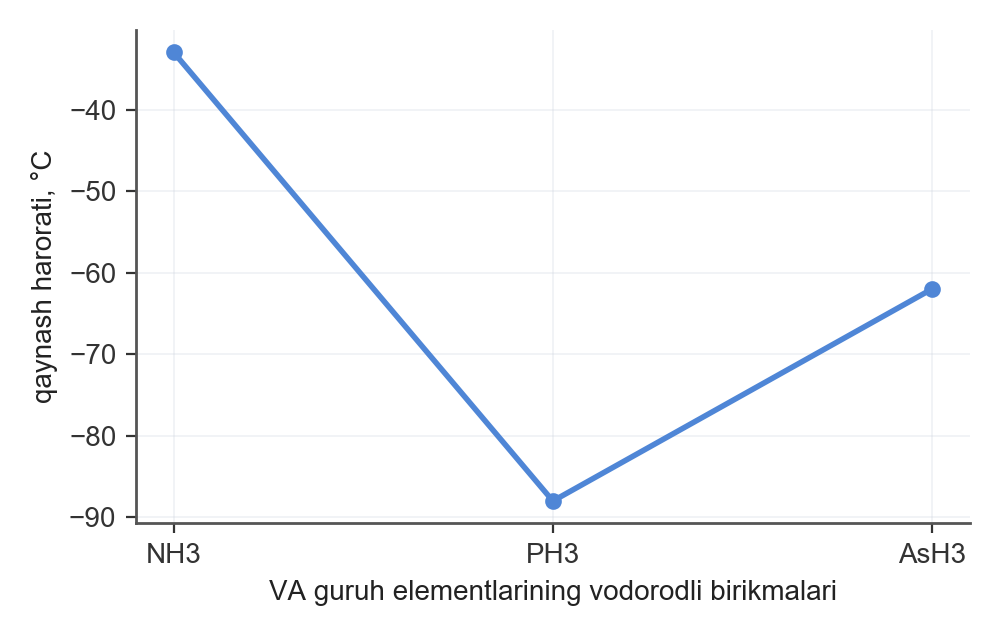
\includegraphics[width=0.86\linewidth]{rasmlar/gen/hy2_v07_0.png}\end{center}
Qaysi birikmaning qaynash harorati qonuniyatdan keskin farq qiladi?

\noindent A)~\textsl{NH\textsubscript{3}} \hfill B)~\textsl{PH\textsubscript{3}} \hfill C)~\textsl{AsH\textsubscript{3}}\par
\qsep
\noindent\qn{11.} Rux (\textit{Z} = 30) atomining tashqi energetik pog`onasidagi elektronlar \textbf{sonini aniqlang.}

\noindent A)~\textsl{3} \hfill B)~\textsl{1} \hfill C)~\textsl{4} \hfill D)~\textsl{2}\par
\qsep
\noindent\qn{12.} A + B $\to$ mahsulot reaksiyada v = k$\cdot$[A]\textsuperscript{2}$\cdot$[B]\textsuperscript{2}. Idish hajmi 2 marta kamaytirilsa (T = const), reaksiya tezligi necha marta o`zgaradi?

\noindent A)~\textsl{4} \hfill B)~\textsl{2} \hfill C)~\textsl{16} \hfill D)~\textsl{32}\par
\qsep
\noindent\qn{13.} Rasmda tasvirlangan A elementi haqida qaysi fikr to`g`ri?
\begin{center}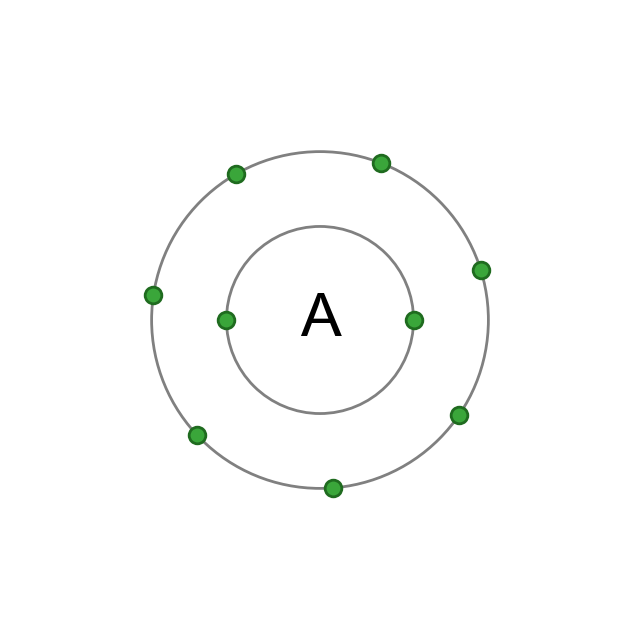
\includegraphics[width=0.86\linewidth]{rasmlar/gen/atom_9_16432.png}\end{center}
\noindent A)~\textsl{Metall, oksidi asosli xossali}\par
\noindent B)~\textsl{Metall, vodorodli birikma hosil qilmaydi}\par
\noindent C)~\textsl{Inert gaz, birikmalar hosil qilmaydi}\par
\noindent D)~\textsl{Metallmas, oksidi kislotali xossali}\par
\qsep
\noindent\qn{14.} 3,1 g fosfor yondirilib, hosil bo`lgan oksid suvda eritildi (ortofosfat kislota), so`ng 0,3 mol NaOH qo`shildi. Hosil bo`lgan Na\textsubscript{3}PO\textsubscript{4} \textbf{massasini (g) aniqlang.}

\noindent A)~\textsl{32,8} \hfill B)~\textsl{16,4} \hfill C)~\textsl{8,2} \hfill D)~\textsl{12}\par
\qsep
\noindent\qn{15.} NaBr + AgNO\textsubscript{3} $\to$ AgBr + NaNO\textsubscript{3} reaksiyasida 51,5 g NaBr ishtirok etdi. AgBr \textbf{miqdorini (mol) toping.}

\noindent A)~\textsl{1} \hfill B)~\textsl{0,25} \hfill C)~\textsl{0,75} \hfill D)~\textsl{0,5}\par
\qsep
\noindent\qn{16.} Ishqoriy metallar haqida qaysi fikrlar to`g`ri? 1) Natriy yonganda Na\textsubscript{2}O\textsubscript{2} hosil bo`ladi; 2) Natriy kerosin ostida saqlanadi; 3) Natriyning olinishi suyuqlanma NaCl elektrolizi bilan; 4) Ishqoriy metallar tabiatda erkin holda uchraydi

\noindent A)~\textsl{2, 4} \hfill B)~\textsl{2, 3} \hfill C)~\textsl{1, 3, 4} \hfill D)~\textsl{1, 2, 3}\par
\qsep
\noindent\qn{17.} Alyuminiy va magniy dan iborat 5,1 g aralashma mo`l xlorid kislotada eritilganda 5,6 l (n.sh.) vodorod ajraldi. Aralashmadagi alyuminiyning massa \textbf{ulushini (\%) aniqlang.}

\noindent A)~\textsl{52,9} \hfill B)~\textsl{47,1} \hfill C)~\textsl{26,5} \hfill D)~\textsl{2,7}\par
\qsep
\noindent\qn{18.} D-metallar va ularning birikmalari haqida qaysi fikrlar to`g`ri? 1) Cu(OH)\textsubscript{2} qizdirilganda CuO ga parchalanadi; 2) Fe(OH)\textsubscript{2} havoda qo`ng`ir rangga o`tadi; 3) Cr\textsubscript{2}O\textsubscript{3} asosli oksid; 4) Mis suyultirilgan HCl bilan reaksiyaga kirishadi

\noindent A)~\textsl{1, 2} \hfill B)~\textsl{4} \hfill C)~\textsl{1, 2, 3} \hfill D)~\textsl{1, 3, 4}\par
\qsep
\noindent\qn{19.} 0,1 mol Ca(HCO\textsubscript{3})\textsubscript{2} tutgan suv qaynatilganda hosil bo`lgan CaCO\textsubscript{3} cho`kma massasini (g)  \textbf{ni toping.}

\noindent A)~\textsl{20} \hfill B)~\textsl{10} \hfill C)~\textsl{5} \hfill D)~\textsl{15}\par
\qsep
\noindent\qn{20.} CH\textsubscript{3}--C(CH\textsubscript{3})\textsubscript{2}--CH\textsubscript{2}--CH\textsubscript{3} birikmaning sistematik nomi qaysi qatorda to`g`ri keltirilgan?

\noindent\begin{tabular}{@{}p{0.47\linewidth}@{}p{0.47\linewidth}@{}}
A)~\textsl{2-metilpentan} & B)~\textsl{3,3-dimetilbutan} \\
C)~\textsl{2,2-dimetilpropan} & D)~\textsl{2,2-dimetilbutan} \\
\end{tabular}\par
\qsep
\noindent\qn{21.} Etilen va asetilendan iborat 5,4 g aralashmani to`liq gidrogenlash uchun sarflanadigan vodorod \textbf{hajmini (l, n.sh.) aniqlang.} Aralashmadagi etilen va asetilenning mol nisbati 1 : 1.

\noindent A)~\textsl{13,44} \hfill B)~\textsl{6,72} \hfill C)~\textsl{3,36} \hfill D)~\textsl{4,48}\par
\qsep
\noindent\qn{22.} Reaksiya tenglamasi: 2C\textsubscript{6}H\textsubscript{6} + 15O\textsubscript{2} $\to$ 12CO\textsubscript{2} + 6H\textsubscript{2}O. Reaksiyaga 32 g O\textsubscript{2} kirishdi. CO\textsubscript{2} \textbf{hajmini (l, n.sh.) hisoblang.}

\noindent A)~\textsl{28} \hfill B)~\textsl{35,84} \hfill C)~\textsl{8,96} \hfill D)~\textsl{17,92}\par
\qsep
\noindent\qn{23.} CH\textsubscript{3}CHO + Ag\textsubscript{2}O (NH\textsubscript{3}) reaksiyasi natijasida qaysi organik modda hosil bo`ladi?

\noindent\begin{tabular}{@{}p{0.47\linewidth}@{}p{0.47\linewidth}@{}}
A)~\textsl{etilatsetat} & B)~\textsl{sirka kislota} \\
C)~\textsl{metan} & D)~\textsl{sirka aldegid} \\
\end{tabular}\par
\qsep
\noindent\qn{24.} Aldegid va ketonlar haqida qaysi fikrlar to`g`ri? 1) Formalin --- formaldegidning 40\% li eritmasi; 2) Sirka aldegid Kucherov reaksiyasi bilan olinadi; 3) Aseton suvda erimaydi; 4) Formaldegid gaz holatda, suvda yaxshi eriydi

\noindent A)~\textsl{1, 3, 4} \hfill B)~\textsl{1, 2, 4} \hfill C)~\textsl{1, 4} \hfill D)~\textsl{2, 3, 4}\par
\qsep
\noindent\qn{25.} Karbon kislotalar haqida qaysi fikrlar to`g`ri? 1) Sirka kislota karbonatlar bilan CO\textsubscript{2} ajratadi; 2) Sirka angidrid ikki molekula sirka kislotadan suv chiqib hosil bo`ladi; 3) Benzoy kislota Na\textsubscript{2}CO\textsubscript{3} bilan reaksiyaga kirishmaydi; 4) Karboksil guruh karbonil va gidroksil guruhlardan iborat

\noindent A)~\textsl{3, 4} \hfill B)~\textsl{2, 3} \hfill C)~\textsl{1, 2, 4} \hfill D)~\textsl{1, 3}\par
\qsep
\noindent\qn{26.} 88 g CH\textsubscript{3}COOC\textsubscript{2}H\textsubscript{5} dan quyidagi ikki bosqichda C\textsubscript{2}H\textsubscript{4} olinadi: 1) CH\textsubscript{3}COOC\textsubscript{2}H\textsubscript{5} + H\textsubscript{2}O $\to$ CH\textsubscript{3}COOH + C\textsubscript{2}H\textsubscript{5}OH (unum 75\%); 2) C\textsubscript{2}H\textsubscript{5}OH $\to$ C\textsubscript{2}H\textsubscript{4} + H\textsubscript{2}O (unum 50\%). Oxirgi mahsulot C\textsubscript{2}H\textsubscript{4} ning \textbf{hajmini (l, n.sh.) toping.}

\noindent A)~\textsl{11,2} \hfill B)~\textsl{16,8} \hfill C)~\textsl{8,4} \hfill D)~\textsl{22,4}\par
\qsep
\noindent\qn{27.} 68,4 g maltoza to`liq gidrolizlanib, hosil bo`lgan mahsulot Ag\textsubscript{2}O ning ammiakli eritmasi bilan oksidlandi. Ajralgan kumush \textbf{massasini (g) aniqlang.}

\noindent A)~\textsl{43,2} \hfill B)~\textsl{172,8} \hfill C)~\textsl{86,4} \hfill D)~\textsl{21,6}\par
\qsep
\noindent\qn{28.} 61,5 g C\textsubscript{6}H\textsubscript{5}NO\textsubscript{2} dan quyidagi ikki bosqichda C\textsubscript{6}H\textsubscript{5}NH\textsubscript{3}Cl olinadi: 1) C\textsubscript{6}H\textsubscript{5}NO\textsubscript{2} + 3H\textsubscript{2} $\to$ C\textsubscript{6}H\textsubscript{5}NH\textsubscript{2} + 2H\textsubscript{2}O (unum 80\%); 2) C\textsubscript{6}H\textsubscript{5}NH\textsubscript{2} + HCl $\to$ C\textsubscript{6}H\textsubscript{5}NH\textsubscript{3}Cl (unum 75\%). Oxirgi mahsulot C\textsubscript{6}H\textsubscript{5}NH\textsubscript{3}Cl ning \textbf{massasini (g) toping.}

\noindent A)~\textsl{48,56} \hfill B)~\textsl{38,85} \hfill C)~\textsl{51,8} \hfill D)~\textsl{64,75}\par
\qsep
\noindent\qn{29.} Vinilxlorid monomeridan olingan polimerning molyar massasi 62500 g/mol. Polimerlanish \textbf{darajasini aniqlang.}

\noindent A)~\textsl{1000} \hfill B)~\textsl{2000} \hfill C)~\textsl{500} \hfill D)~\textsl{1010}\par
\qsep
\noindent\qn{30.} Rasmdagi asbobda oxirgi idishga NaOH eritmasi solingan. Uning vazifasi nima?
\begin{center}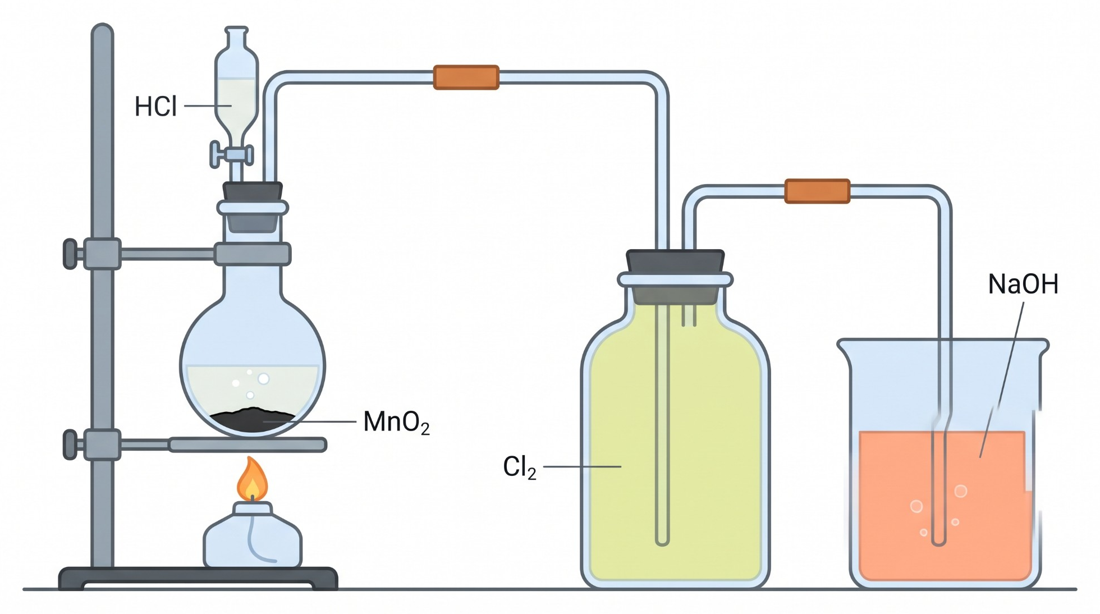
\includegraphics[width=0.86\linewidth]{rasmlar/darslik/d_xlor.png}\end{center}
\noindent A)~\textsl{xlorni suvda eritish}\par
\noindent B)~\textsl{ortiqcha xlorni yutib, atrof-muhitni zaharlanishdan saqlash}\par
\noindent C)~\textsl{xlorni quritish}\par
\noindent D)~\textsl{reaksiyani tezlashtirish}\par
\qsep
\noindent\qn{31.} I\textsuperscript{$-$} ionini aniqlash uchun qaysi reagent mos va qanday belgi kuzatiladi?
\noindent A)~\textsl{AgNO\textsubscript{3}: sariq cho`kma (AgI), HNO\textsubscript{3} da erimaydi}\par
\noindent B)~\textsl{NaOH: qo`ng`ir cho`kma (Fe(OH)\textsubscript{3})}\par
\noindent C)~\textsl{HCl: rangsiz gaz (CO\textsubscript{2}) ajraladi}\par
\noindent D)~\textsl{AgNO\textsubscript{3}: sariq cho`kma (Ag\textsubscript{3}PO\textsubscript{4}), HNO\textsubscript{3} da eriydi}\par
\qsep
\noindent\qn{32.} Uch probirkada (\textit{X}, \textit{Y}, \textit{Z}) Na\textsubscript{2}SO\textsubscript{4}, K\textsubscript{2}CO\textsubscript{3}, NH\textsubscript{4}Cl eritmalari bor (tartibsiz). Ularga HCl va NaOH ta'sir ettirildi. Kuzatuvlar jadvalda:
\begin{center}
\renewcommand{\arraystretch}{1.15}
\fitbox{\begin{tabular}{|c|c|c|}\hline
\textbf{Probirka} & \textbf{HCl qo`shilganda} & \textbf{NaOH qo`shib qizdirilganda} \\ \hline
\textit{X} & gaz ajraladi & o`zgarish yo`q \\ \hline
\textit{Y} & o`zgarish yo`q & o`tkir hidli gaz ajraladi \\ \hline
\textit{Z} & o`zgarish yo`q & o`zgarish yo`q \\ \hline
\end{tabular}}
\end{center}
\textit{X}, \textit{Y}, \textit{Z} probirkalardagi \textbf{moddalarni aniqlang.}
\noindent A)~\textsl{\textit{X} -- NH\textsubscript{4}Cl, \textit{Y} -- Na\textsubscript{2}SO\textsubscript{4}, \textit{Z} -- K\textsubscript{2}CO\textsubscript{3}}\par
\noindent B)~\textsl{\textit{X} -- Na\textsubscript{2}SO\textsubscript{4}, \textit{Y} -- NH\textsubscript{4}Cl, \textit{Z} -- K\textsubscript{2}CO\textsubscript{3}}\par
\noindent C)~\textsl{\textit{X} -- NH\textsubscript{4}Cl, \textit{Y} -- K\textsubscript{2}CO\textsubscript{3}, \textit{Z} -- Na\textsubscript{2}SO\textsubscript{4}}\par
\noindent D)~\textsl{\textit{X} -- K\textsubscript{2}CO\textsubscript{3}, \textit{Y} -- NH\textsubscript{4}Cl, \textit{Z} -- Na\textsubscript{2}SO\textsubscript{4}   ---}\par
\qsep
\end{multicols}
\medskip
\noindent\setlength{\fboxsep}{0pt}\fbox{\begin{tabular}{p{0.74\linewidth}|p{0.2\linewidth}}
\parbox[t]{0.72\linewidth}{\vspace{3pt}\textbf{Topshiriqlar (33--35) va javob variant (A--F)larini o`zaro to`g`ri moslashtiring.} NaHCO\textsubscript{3} va KHCO\textsubscript{3} dan iborat 36,8 g aralashma mo`l xlorid kislota bilan to`liq reaksiyaga kirishdi.
\vspace{3pt}} & \parbox[t]{0.19\linewidth}{\vspace{3pt}A~\textsl{32}\\[3pt]
B~\textsl{8,96}\\[3pt]
C~\textsl{40}\\[3pt]
D~\textsl{116,8}\\[3pt]
E~\textsl{146}\\[3pt]
F~\textsl{7,17}}\\ \hline
\parbox[t]{0.72\linewidth}{\vspace{2pt}\textbf{33. Ajralgan gaz hajmini (l, n.sh.) aniqlang.}\vspace{2pt}} & \\ \hline
\parbox[t]{0.72\linewidth}{\vspace{2pt}\textbf{34. Aralashmani to`liq eritish uchun sarflangan 10\% li HCl eritmasining massasini (g) aniqlang (M(HCl) = 36,5 g/mol).}\vspace{2pt}} & \\ \hline
\parbox[t]{0.72\linewidth}{\vspace{2pt}\textbf{35. Ajralgan gaz mo`l Ca(OH)\textsubscript{2} eritmasidan o`tkazilganda hosil bo`lgan cho`kma massasini (g) aniqlang.}\vspace{2pt}} & 
\end{tabular}}
\par\bigskip
\noindent\qn{36.} KMnO\textsubscript{4} + KI + H\textsubscript{2}SO\textsubscript{4} $\to$ MnSO\textsubscript{4} + I\textsubscript{2} + K\textsubscript{2}SO\textsubscript{4} + H\textsubscript{2}O reaksiya tenglamasini elektron balans usulida tenglang va barcha koeffitsiyentlar \textbf{yig`indisini aniqlang.}
\javob\qsep
\noindent\qn{37.} AgNO\textsubscript{3} eritmasi inert elektrodlar yordamida 2 A tok kuchi bilan 965 s elektroliz qilindi. Anodda ajralgan O\textsubscript{2} hajmi (l, n.sh.) \textbf{ni toping.}
\javob\qsep
\noindent\qn{38.} 47 g Cu(NO\textsubscript{3})\textsubscript{2} to`liq parchalanguncha qizdirildi. Qattiq qoldiq \textbf{massasini (g) aniqlang.}
\javob\qsep
\noindent\qn{39.} 12 g sirka kislotani neytrallash uchun 10\% li NaOH eritmasidan necha gramm kerak?
\javob\qsep
\noindent\qn{40.} 12,3 g nitrobenzol anilinga qaytarildi (unum 80\%), hosil bo`lgan anilin mo`l bromli suv bilan reaksiyaga kirishdi (unum 80\%). Hosil bo`lgan 2,4,6-tribromanilin (M = 330 g/mol) \textbf{massasini (g) toping.}
\javob\qsep
\par\bigskip\begin{center}\textbf{\fontsize{13}{15}\selectfont YOZMA ISH}\end{center}
\noindent\qn{41.} \textbf{Topshiriqni bajarish jarayonida barcha reaksiya tenglamalarini yozing. Miqdoriy va arifmetik hisoblashlarni (unga asos bo`lgan usul yoki formulani ko`rsatgan holda) uzviy ketma-ketlikda bajaring.}\par\smallskip
29,25 g NaCl 300 g suvda eritildi. Hosil bo`lgan eritma inert elektrodlar yordamida 20 A tok kuchi bilan 965 s davomida elektroliz qilindi.\par
\noindent 1)\ Elektroliz tenglamasini yozing. Katodda va anodda ajralgan gazlarning hajmini (l, n.sh.) hisoblang (F = 96500 C/mol).\par
\noindent 2)\ Elektroliz qilingan NaCl ning massasini (g) toping. Elektroliz davomida o`tgan zaryadni (C) ham hisoblang.\par
\noindent 3)\ Elektroliz tugagach eritmadagi NaOH va qolgan NaCl ning massa ulushlarini (\%) aniqlang.\par
\noindent 4)\ Anodda ajralgan gaz mo`l KI eritmasidan o`tkazildi. Ajralgan yodning massasini (g) hisoblang (reaksiya tenglamasini yozing). Neytrallash uchun sarflangan HCl miqdorini (mol) ham toping.\par
\noindent 5)\ Elektroliz tugagan eritmani to`liq neytrallash uchun 10\% li HCl eritmasidan necha gramm kerak? Elektroliz tugagan eritmadan CO\textsubscript{2} o`rta tuz (karbonat) hosil bo`lguncha yuttirilsa, hosil bo`ladigan karbonat massasini (g) ham hisoblang.\par
\diqqat{Mazkur topshiriq kengaytirilgan javobni talab etib, uning yechilish usuli va shu usul asosidagi barcha hisoblash amallari javoblar varaqasida aks etishi lozim.}\qsep
\noindent\qn{42.} Quyidagi o`zgarishlar zanjirida \textit{X}, \textit{Y}, \textit{Z} noma'lum organik moddalar:\par
\[\setlength{\fboxsep}{0pt}\text{C\textsubscript{2}H\textsubscript{2}}\xrightarrow{\text{H\textsubscript{2}O, Hg\textsuperscript{2+}}}\text{\textit{X}}\xrightarrow{\text{Ag\textsubscript{2}O, NH\textsubscript{3}}}\text{\textit{Y}}\xrightarrow{\text{Cl\textsubscript{2}, P}}\text{ClCH\textsubscript{2}COOH}\]
\noindent 1)\ C\textsubscript{2}H\textsubscript{2} $\to$ \textit{X} : reaksiya tenglamasini yozing; hosil bo`lgan moddani nomlang.\par
\noindent 2)\ \textit{X} $\to$ \textit{Y} : reaksiya tenglamasini yozing; hosil bo`lgan moddani nomlang.\par
\noindent 3)\ \textit{Y} $\to$ ClCH\textsubscript{2}COOH : reaksiya tenglamasini yozing; hosil bo`lgan moddani nomlang.\par
\diqqat{Mazkur topshiriq kengaytirilgan javobni talab etib, uning yechilish usuli va shu usul asosidagi barcha hisoblash amallari javoblar varaqasida aks etishi lozim.}\qsep
\noindent\qn{43.} \textbf{Topshiriqni bajarish jarayonida barcha reaksiya tenglamalarini yozing. Miqdoriy va arifmetik hisoblashlarni (unga asos bo`lgan usul yoki formulani ko`rsatgan holda) uzviy ketma-ketlikda bajaring.}\par\smallskip
11,2 g temir mo`l xlorda yondirildi. Hosil bo`lgan tuz suvda eritilib, avval ishqor bilan, so`ng boshqa porsiyasi KI eritmasi bilan ta'sirlashtirildi.\par
\noindent 1)\ Reaksiya tenglamasini yozing. Sarflangan xlor hajmini (l, n.sh.) va hosil bo`lgan tuz massasini (g) toping. Hosil bo`lgan FeCl\textsubscript{3} miqdorini (mol) ham toping.\par
\noindent 2)\ Tuz eritmasiga mo`l NaOH qo`shilganda hosil bo`lgan cho`kma massasini (g) aniqlang.\par
\noindent 3)\ Cho`kma qizdirilganda hosil bo`ladigan oksid massasini (g) hisoblang.\par
\noindent 4)\ Tuzning shunday miqdoriga mo`l KI qo`shilganda ajraladigan yod massasini (g) toping (2FeCl\textsubscript{3} + 2KI $\to$ 2FeCl\textsubscript{2} + 2KCl + I\textsubscript{2}).\par
\noindent 5)\ Hosil bo`lgan FeCl\textsubscript{3} eritmasiga temir qo`shilib FeCl\textsubscript{2} hosil qilindi (2FeCl\textsubscript{3} + Fe $\to$ 3FeCl\textsubscript{2}). Sarflangan temir massasini (g) toping.\par
\diqqat{Mazkur topshiriq kengaytirilgan javobni talab etib, uning yechilish usuli va shu usul asosidagi barcha hisoblash amallari javoblar varaqasida aks etishi lozim.}\qsep
\newpage
\renewcommand{\curvar}{8-variant}
\thispagestyle{first}
\noindent\textit{Davriy jadvaldan foydalanish mumkin.}
\par\smallskip
\begin{multicols}{2}
\noindent\qn{1.} Qotishmaning massa bo`yicha tarkibi doira diagrammasida ko`rsatilgan.
\begin{center}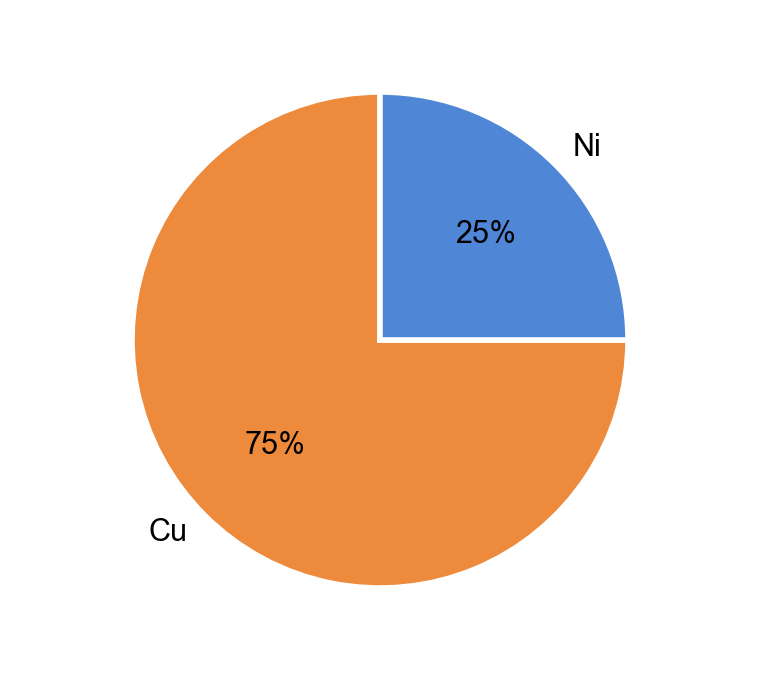
\includegraphics[width=0.86\linewidth]{rasmlar/gen/pi_v08_0.png}\end{center}
200 g qotishmadagi Ni \textbf{massasini (g) toping.}

\noindent A)~\textsl{150} \hfill B)~\textsl{50} \hfill C)~\textsl{100} \hfill D)~\textsl{5000}\par
\qsep
\noindent\qn{2.} H\textsubscript{2}O\textsubscript{2} moddaning parchalanish reaksiyasida konsentratsiyaning vaqt bo`yicha o`zgarishi jadvalda berilgan:
\begin{center}
\renewcommand{\arraystretch}{1.15}
\fitbox{\begin{tabular}{|c|c|}\hline
\textbf{t, min} & \textbf{c, mol/l} \\ \hline
0 & 2,4 \\ \hline
2 & 2,04 \\ \hline
4 & 1,68 \\ \hline
6 & 1,32 \\ \hline
\end{tabular}}
\end{center}
0-minutdan 2-minutgacha o`rtacha tezlikni mol/(l$\cdot$min) \textbf{hisoblang.}

\noindent A)~\textsl{0,36} \hfill B)~\textsl{0,09} \hfill C)~\textsl{1,2} \hfill D)~\textsl{0,18}\par
\qsep
\noindent\qn{3.} 40 l H\textsubscript{2} va 40 l O\textsubscript{2} aralashmasi reaksiyaga kirishdi (2H\textsubscript{2} + O\textsubscript{2} $\to$ 2H\textsubscript{2}O, hamma moddalar bir xil sharoitda gaz holida, suv bug` holida). Reaksiyadan keyingi gaz aralashmasining \textbf{hajmini (l) aniqlang.}

\noindent A)~\textsl{80} \hfill B)~\textsl{60} \hfill C)~\textsl{40} \hfill D)~\textsl{20}\par
\qsep
\noindent\qn{4.} Brom atomida d-pog`onachadagi elektronlar \textbf{sonini aniqlang} (\textit{Z} = 35).

\noindent A)~\textsl{11} \hfill B)~\textsl{9} \hfill C)~\textsl{10} \hfill D)~\textsl{12}\par
\qsep
\noindent\qn{5.} pH = 3 bo`lgan HCl eritmasining 100 ml siga pH = 11 bo`lgan NaOH eritmasidan 100 ml qo`shildi. Hosil bo`lgan eritmaning pH \textbf{qiymatini aniqlang.}

\noindent A)~\textsl{3} \hfill B)~\textsl{11} \hfill C)~\textsl{4} \hfill D)~\textsl{7}\par
\qsep
\noindent\qn{6.} 35-tartib raqamli element atomida magnit kvant soni m\_l = 1 bo`lgan elektronlardan nechtasining spin kvant soni m\_s = +$\frac{1}{2}$ ga, nechtasiniki m\_s = $-$$\frac{1}{2}$ ga teng?

\noindent A)~\textsl{3 va 4} \hfill B)~\textsl{5 va 3} \hfill C)~\textsl{4 va 4} \hfill D)~\textsl{4 va 3}\par
\qsep
\noindent\qn{7.} MgSO\textsubscript{4}$\cdot$7H\textsubscript{2}O kristallogidratida kristallizatsion suvning massa \textbf{ulushini (\%) aniqlang.}

\noindent A)~\textsl{51,2} \hfill B)~\textsl{48,8} \hfill C)~\textsl{25,6} \hfill D)~\textsl{105}\par
\qsep
\noindent\qn{8.} 40 g NaOH 250 g suvda eritildi. Eritmaning molyal \textbf{konsentratsiyasini (mol/kg) aniqlang.}

\noindent A)~\textsl{4} \hfill B)~\textsl{3,45} \hfill C)~\textsl{0} \hfill D)~\textsl{8}\par
\qsep
\noindent\qn{9.} 50 g CuSO\textsubscript{4}$\cdot$5H\textsubscript{2}O 100 g suvda eritildi. Eritmadagi tuzning massa \textbf{ulushini (\%) aniqlang.}

\noindent A)~\textsl{32} \hfill B)~\textsl{21,33} \hfill C)~\textsl{33,33} \hfill D)~\textsl{42,67}\par
\qsep
\noindent\qn{10.} 13,9 g FeSO\textsubscript{4}$\cdot$7H\textsubscript{2}O 100 g suvda eritildi. Eritmadagi tuzning massa \textbf{ulushini (\%) aniqlang.}

\noindent A)~\textsl{6,67} \hfill B)~\textsl{7,6} \hfill C)~\textsl{12,2} \hfill D)~\textsl{13,35}\par
\qsep
\noindent\qn{11.} Quyidagi zarrachalardan qaysilari argon atomi bilan izoelektron? 1) O\textsuperscript{2$-$}; 2) Cl\textsuperscript{$-$}; 3) Na\textsuperscript{+}; 4) Ca\textsuperscript{2+}

\noindent A)~\textsl{1, 3} \hfill B)~\textsl{3, 4} \hfill C)~\textsl{2, 4} \hfill D)~\textsl{1, 2}\par
\qsep
\noindent\qn{12.} 2 mol HNO\textsubscript{3} va 2 mol Ba(OH)\textsubscript{2} suvda eritilib, eritma hajmi 5 l ga yetkazildi. Eritmadagi barcha ionlarning umumiy molyar \textbf{konsentratsiyasini (mol/l) aniqlang} (kuchli elektrolitlar to`liq dissotsilanadi).

\noindent A)~\textsl{0,8} \hfill B)~\textsl{4} \hfill C)~\textsl{2} \hfill D)~\textsl{1}\par
\qsep
\noindent\qn{13.} N\textsubscript{2} + 3H\textsubscript{2} $\rightleftarrows$ 2NH\textsubscript{3} reaksiyasi 4 l hajmli idishda o`tkazildi. Moddalar miqdori jadvalda berilgan:
\begin{center}
\renewcommand{\arraystretch}{1.15}
\fitbox{\begin{tabular}{|c|c|c|c|}\hline
\textbf{Modda} & \textbf{N\textsubscript{2}} & \textbf{H\textsubscript{2}} & \textbf{NH\textsubscript{3}} \\ \hline
Boshlang`ich miqdor, mol & 4 & 6 & 0 \\ \hline
Muvozanatdagi miqdor, mol & --- & --- & 2 \\ \hline
\end{tabular}}
\end{center}
Muvozanat \textbf{konstantasini (K) hisoblang.}

\noindent A)~\textsl{1,58} \hfill B)~\textsl{0,395} \hfill C)~\textsl{3,16} \hfill D)~\textsl{0,79}\par
\qsep
\noindent\qn{14.} 4Li + O\textsubscript{2} $\to$ 2Li\textsubscript{2}O jarayoni uchun 64 g O\textsubscript{2} olingan. Li\textsubscript{2}O \textbf{massasini (g) aniqlang.}

\noindent A)~\textsl{30} \hfill B)~\textsl{120} \hfill C)~\textsl{240} \hfill D)~\textsl{60}\par
\qsep
\noindent\qn{15.} 0,4 mol Ca(OH)\textsubscript{2} tutgan eritmadan 0,6 mol karbonat angidrid o`tkazildi. Eritmada qolgan kalsiy gidrokarbonatning \textbf{massasini (g) aniqlang.}

\noindent A)~\textsl{32,4} \hfill B)~\textsl{40} \hfill C)~\textsl{97,2} \hfill D)~\textsl{20}\par
\qsep
\noindent\qn{16.} D-metallar va ularning birikmalari haqida qaysi fikrlar to`g`ri? 1) Fe(OH)\textsubscript{2} havoda qo`ng`ir rangga o`tadi; 2) Xrom (VI) oksidi (CrO\textsubscript{3}) kislotali oksid; 3) Rux eritmada Fe\textsuperscript{2+} ni siqib chiqara olmaydi; 4) Cr\textsubscript{2}O\textsubscript{3} asosli oksid

\noindent A)~\textsl{1, 3} \hfill B)~\textsl{1, 4} \hfill C)~\textsl{2, 3} \hfill D)~\textsl{1, 2}\par
\qsep
\noindent\qn{17.} Ca(HCO\textsubscript{3})\textsubscript{2} $\to$ CaCO\textsubscript{3} + CO\textsubscript{2} + H\textsubscript{2}O jarayoni uchun tarkibida 80\% aralashma bo`lgan 81 g namuna (asosiy modda Ca(HCO\textsubscript{3})\textsubscript{2}) olingan. CO\textsubscript{2} \textbf{hajmini (l, n.sh.) aniqlang.}

\noindent A)~\textsl{4,48} \hfill B)~\textsl{1,12} \hfill C)~\textsl{2,24} \hfill D)~\textsl{3,36}\par
\qsep
\noindent\qn{18.} CaO + CO\textsubscript{2} $\to$ CaCO\textsubscript{3} jarayoni uchun 4,48 l (n.sh.) CO\textsubscript{2} olingan. CaCO\textsubscript{3} \textbf{miqdorini (mol) aniqlang.}

\noindent A)~\textsl{0,4} \hfill B)~\textsl{0,2} \hfill C)~\textsl{0,1} \hfill D)~\textsl{0,3}\par
\qsep
\noindent\qn{19.} Ca $\to$ ? $\to$ ? $\to$ ? o`zgarishlar zanjirida (reagentlar: O\textsubscript{2}, H\textsubscript{2}O, CO\textsubscript{2}) 1-bosqichda hosil bo`ladigan modda \textbf{formulasini toping.}

\noindent A)~\textsl{NaCl} \hfill B)~\textsl{CaO} \hfill C)~\textsl{K\textsubscript{3}PO\textsubscript{4}} \hfill D)~\textsl{H\textsubscript{2}SO\textsubscript{3}}\par
\qsep
\noindent\qn{20.} 0,1 mol metan xlor bilan to`liq xlorlanib, CCl\textsubscript{4} olindi. Sarflangan xlor \textbf{hajmini (l, n.sh.) aniqlang.}

\noindent A)~\textsl{8,96} \hfill B)~\textsl{2,24} \hfill C)~\textsl{4,48} \hfill D)~\textsl{6,72}\par
\qsep
\noindent\qn{21.} 23 g C\textsubscript{2}H\textsubscript{5}OH dan quyidagi ikki bosqichda C\textsubscript{2}H\textsubscript{6} olinadi: 1) C\textsubscript{2}H\textsubscript{5}OH $\to$ C\textsubscript{2}H\textsubscript{4} + H\textsubscript{2}O (unum 50\%); 2) C\textsubscript{2}H\textsubscript{4} + H\textsubscript{2} $\to$ C\textsubscript{2}H\textsubscript{6} (unum 50\%). Oxirgi mahsulot C\textsubscript{2}H\textsubscript{6} ning \textbf{hajmini (l, n.sh.) toping.}

\noindent A)~\textsl{5,6} \hfill B)~\textsl{11,2} \hfill C)~\textsl{1,4} \hfill D)~\textsl{2,8}\par
\qsep
\noindent\qn{22.} Arenlar, neft va tabiiy gaz haqida qaysi fikrlar to`g`ri? 1) Benzolda 6 ta sp\textsuperscript{2} gibridlangan uglerod bor; 2) Benzoldan nitrobenzol nitrolash bilan olinadi; 3) Benzol uchun birikish reaksiyalari mutlaqo xos emas; 4) Benzol bromli suvni rangsizlantirmaydi

\noindent A)~\textsl{1, 2, 4} \hfill B)~\textsl{1, 4} \hfill C)~\textsl{1, 3} \hfill D)~\textsl{3, 4}\par
\qsep
\noindent\qn{23.} C\textsubscript{2}H\textsubscript{5}Cl + KOH $\to$ C\textsubscript{2}H\textsubscript{5}OH + KCl reaksiyasida 5,6 g KOH ishtirok etdi. KCl \textbf{massasini (g) toping.}

\noindent A)~\textsl{14,9} \hfill B)~\textsl{3,73} \hfill C)~\textsl{7,45} \hfill D)~\textsl{11,18}\par
\qsep
\noindent\qn{24.} 3 g metanal Ag\textsubscript{2}O ning ammiakli eritmasi bilan to`liq oksidlanganda hosil bo`lgan kumush \textbf{massasini (g) aniqlang.}

\noindent A)~\textsl{10,8} \hfill B)~\textsl{43,2} \hfill C)~\textsl{86,4} \hfill D)~\textsl{21,6}\par
\qsep
\noindent\qn{25.} Karbon kislotalar haqida qaysi fikrlar to`g`ri? 1) Sirka angidrid ikki molekula sirka kislotadan suv chiqib hosil bo`ladi; 2) Karboksil guruh karbonil va gidroksil guruhlardan iborat; 3) Olein kislota Br\textsubscript{2} ni biriktiradi; 4) Chumoli kislota "kumush ko`zgu" reaksiyasini beradi

\noindent\begin{tabular}{@{}p{0.47\linewidth}@{}p{0.47\linewidth}@{}}
A)~\textsl{1, 2, 3} & B)~\textsl{2, 3, 4} \\
C)~\textsl{1, 2, 3, 4} & D)~\textsl{1, 3, 4} \\
\end{tabular}\par
\qsep
\noindent\qn{26.} Murakkab efirlar va yog`lar haqida qaysi fikrlar to`g`ri? 1) Dietil efir spirtdan yuqori haroratda qaynaydi; 2) Suyuq yog`larni gidrogenlab qattiq yog` olinadi; 3) Suyuq yog`lar to`yinmagan kislotalardan hosil bo`lgan; 4) Murakkab efirlarning gidrolizi ishqoriy muhitda qaytmas

\noindent A)~\textsl{1, 4} \hfill B)~\textsl{2, 3} \hfill C)~\textsl{1, 2} \hfill D)~\textsl{2, 3, 4}\par
\qsep
\noindent\qn{27.} Quyidagi birikmalardan qaysi biri amin sinfiga kiradi?

\noindent A)~\textsl{CH\textsubscript{3}COOH} \hfill B)~\textsl{C\textsubscript{2}H\textsubscript{5}NH\textsubscript{2}} \hfill C)~\textsl{C\textsubscript{12}H\textsubscript{22}O\textsubscript{11}} \hfill D)~\textsl{C\textsubscript{6}H\textsubscript{5}OH}\par
\qsep
\noindent\qn{28.} 4CH\textsubscript{3}NH\textsubscript{2} + 9O\textsubscript{2} $\to$ 4CO\textsubscript{2} + 10H\textsubscript{2}O + 2N\textsubscript{2} reaksiyasida 4,48 l (n.sh.) CH\textsubscript{3}NH\textsubscript{2} ishtirok etdi. O\textsubscript{2} \textbf{hajmini (l, n.sh.) toping.}

\noindent A)~\textsl{1,99} \hfill B)~\textsl{20,16} \hfill C)~\textsl{5,04} \hfill D)~\textsl{10,08}\par
\qsep
\noindent\qn{29.} Rasmda organik birikmaning tuzilish formulasi keltirilgan.
\begin{center}
\includegraphics[width=0.86\linewidth]{rasmlar/gen/fg_475166.png}\end{center}
Molekuladagi uglerod atomlari \textbf{sonini aniqlang.}

\noindent A)~\textsl{5} \hfill B)~\textsl{6} \hfill C)~\textsl{4} \hfill D)~\textsl{7}\par
\qsep
\noindent\qn{30.} Kimyo laboratoriyasida ishlash qoidalari haqida qaysi fikrlar to`g`ri? 1) Ortiqcha reaktiv idishga qaytariladi; 2) Reaktivlarni tatib ko`rish mumkin; 3) Suvni konsentrlangan kislotaga tez quyish mumkin; 4) Zaharli gaz ajraladigan tajriba mo`rili shkafda o`tkaziladi

\noindent A)~\textsl{1, 4} \hfill B)~\textsl{3, 4} \hfill C)~\textsl{4} \hfill D)~\textsl{2, 4}\par
\qsep
\noindent\qn{31.} Rasmdagi asbobda 23,4 g NaCl ga konsentrlangan H\textsubscript{2}SO\textsubscript{4} ta'sir ettirib qizdirildi (NaCl + H\textsubscript{2}SO\textsubscript{4} $\to$ NaHSO\textsubscript{4} + HCl). Ajralgan HCl \textbf{hajmini (l, n.sh.) aniqlang.}
\begin{center}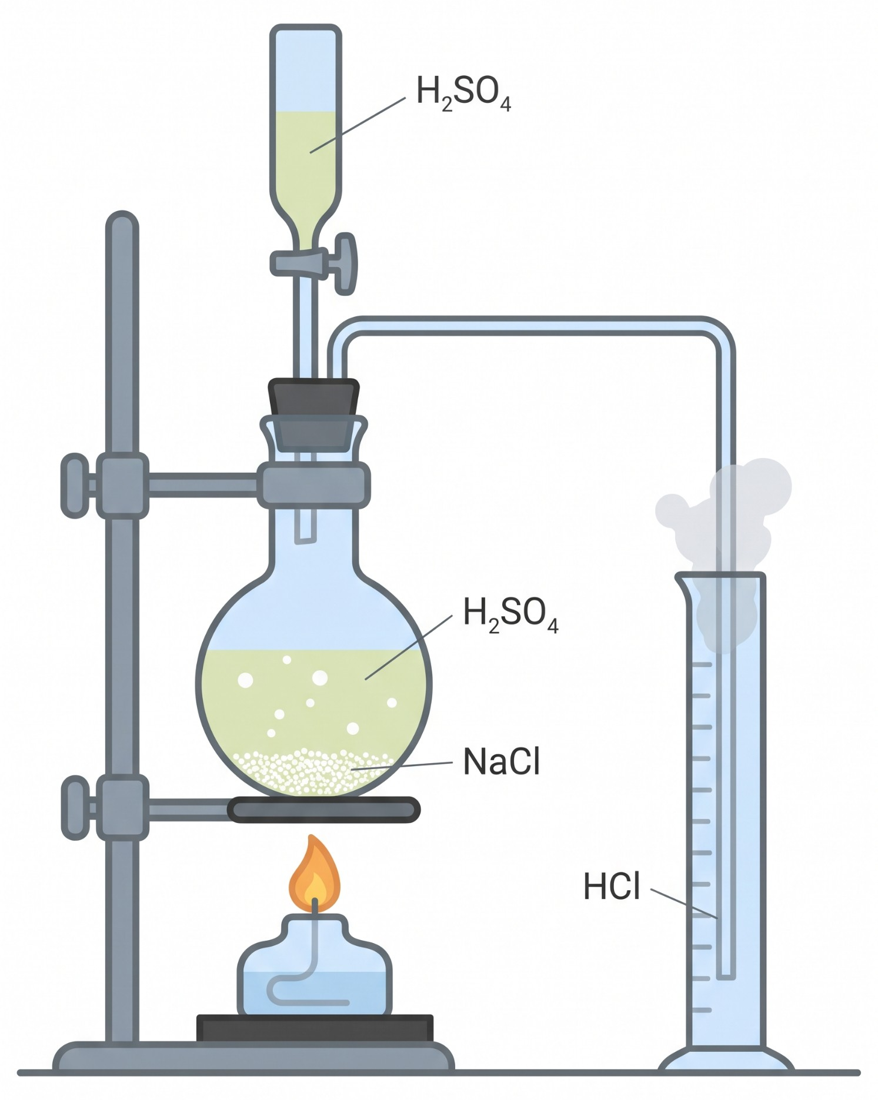
\includegraphics[width=0.86\linewidth]{rasmlar/darslik/d_hcl_lab.png}\end{center}

\noindent A)~\textsl{8,96} \hfill B)~\textsl{17,92} \hfill C)~\textsl{4,48} \hfill D)~\textsl{0,64}\par
\qsep
\noindent\qn{32.} 400 g 12\% li NaCl eritmasidan 100 g suv bug`latildi. Qolgan eritmadagi tuzning massa \textbf{ulushini (\%) toping.}

\noindent\begin{tabular}{@{}p{0.47\linewidth}@{}p{0.47\linewidth}@{}}
A)~\textsl{9,6} & B)~\textsl{3} \\
C)~\textsl{16} & D)~\textsl{12,8   ---} \\
\end{tabular}\par
\qsep
\end{multicols}
\medskip
\noindent\setlength{\fboxsep}{0pt}\fbox{\begin{tabular}{p{0.74\linewidth}|p{0.2\linewidth}}
\parbox[t]{0.72\linewidth}{\vspace{3pt}\textbf{Topshiriqlar (33--35) va javob variant (A--F)larini o`zaro to`g`ri moslashtiring.} Na va Na\textsubscript{2}O dan iborat 17 g aralashma 100 g suvda to`liq eritildi, bunda 2,24 l (n.sh.) vodorod ajraldi. Hosil bo`lgan eritma sirka kislota bilan to`liq neytrallandi.
\vspace{3pt}} & \parbox[t]{0.19\linewidth}{\vspace{3pt}A~\textsl{12,4}\\[3pt]
B~\textsl{20,55}\\[3pt]
C~\textsl{30,82}\\[3pt]
D~\textsl{180}\\[3pt]
E~\textsl{90}\\[3pt]
F~\textsl{24,8}}\\ \hline
\parbox[t]{0.72\linewidth}{\vspace{2pt}\textbf{33. Hosil bo`lgan eritmadagi NaOH ning massa ulushini (\%) aniqlang.}\vspace{2pt}} & \\ \hline
\parbox[t]{0.72\linewidth}{\vspace{2pt}\textbf{34. Dastlabki aralashmadagi Na\textsubscript{2}O massasini (g) aniqlang.}\vspace{2pt}} & \\ \hline
\parbox[t]{0.72\linewidth}{\vspace{2pt}\textbf{35. Neytrallash uchun sarflangan 20\% li sirka kislota eritmasining massasini (g) aniqlang.}\vspace{2pt}} & 
\end{tabular}}
\par\bigskip
\noindent\qn{36.} Mg + HNO\textsubscript{3} $\to$ Mg(NO\textsubscript{3})\textsubscript{2} + NH\textsubscript{4}NO\textsubscript{3} + H\textsubscript{2}O reaksiya tenglamasini elektron balans usulida tenglang va barcha koeffitsiyentlar \textbf{yig`indisini aniqlang.}
\javob\qsep
\noindent\qn{37.} CH\textsubscript{4} va H\textsubscript{2} dan iborat 20 ml aralashma mo`l kisloroda yondirildi (suv suyuq holatda; hajmlar bir xil sharoitda o`lchandi). Reaksiyadan so`ng gazlar hajmi 35 ml ga kamaydi. Aralashmadagi CH\textsubscript{4} \textbf{hajmini (ml) toping.}
\javob\qsep
\noindent\qn{38.} 6,2 g fosfor yondirib hosil bo`lgan oksid suvda eritildi, so`ng eritmaga 0,3 mol NaOH qo`shildi (NaOH : H\textsubscript{3}PO\textsubscript{4} = 1,5 : 1). Hosil bo`lgan tuzlar umumiy \textbf{massasini (g) toping.}
\javob\qsep
\noindent\qn{39.} Uglevodorodning 5,6 g massasi yondirilganda 17,6 g CO\textsubscript{2} va 7,2 g H\textsubscript{2}O hosil bo`ldi. Uglevodorodning molyar \textbf{massasini (g/mol) aniqlang.}
\javob\qsep
\noindent\qn{40.} Polietilen polimerining (polimerlanish darajasi 2000) 280 g namunasini olish uchun polimerlanish unumi 90\% bo`lganda qancha monomer (C\textsubscript{2}H\textsubscript{4}) kerak (g)?
\javob\qsep
\par\bigskip\begin{center}\textbf{\fontsize{13}{15}\selectfont YOZMA ISH}\end{center}
\noindent\qn{41.} \textbf{Topshiriqni bajarish jarayonida barcha reaksiya tenglamalarini yozing. Miqdoriy va arifmetik hisoblashlarni (unga asos bo`lgan usul yoki formulani ko`rsatgan holda) uzviy ketma-ketlikda bajaring.}\par\smallskip
CO va CO\textsubscript{2} dan iborat gazlar aralashmasi (n.sh.) 4,48 l hajm egallaydi va massasi 7,2 g.\par
\noindent 1)\ Aralashmadagi gazlarning mol miqdorlarini hisoblang.\par
\noindent 2)\ Aralashmaning vodorodga nisbatan zichligini va gazlarning hajmiy ulushlarini (\%) aniqlang. Aralashmaning to`liq massasini (g) ham ayting.\par
\noindent 3)\ Aralashmani to`liq yoqish uchun zarur kislorod hajmini (l, n.sh.) toping.\par
\noindent 4)\ Yonishdan keyingi gazlar mo`l NaOH eritmasidan o`tkazildi. Hosil bo`lgan Na\textsubscript{2}CO\textsubscript{3} massasini (g) hisoblang (CO\textsubscript{2} + 2NaOH $\to$ Na\textsubscript{2}CO\textsubscript{3} + H\textsubscript{2}O). NaOH sarfini (g) ham toping.\par
\noindent 5)\ Aralashmaning o`rtacha molyar massasini (g/mol) toping. Shu miqdor CO ni yoqish uchun havo (21\% O\textsubscript{2}) hajmi qancha (l, n.sh.)?\par
\diqqat{Mazkur topshiriq kengaytirilgan javobni talab etib, uning yechilish usuli va shu usul asosidagi barcha hisoblash amallari javoblar varaqasida aks etishi lozim.}\qsep
\noindent\qn{42.} Quyidagi o`zgarishlar zanjirida \textit{X}, \textit{Y}, \textit{Z} noma'lum organik moddalar:\par
\[\setlength{\fboxsep}{0pt}\text{CH\textsubscript{4}}\xrightarrow{\text{Cl\textsubscript{2}, yorug`lik}}\text{\textit{X}}\xrightarrow{\text{Na}}\text{\textit{Y}}\xrightarrow{\text{Cl\textsubscript{2}, yorug`lik}}\text{C\textsubscript{2}H\textsubscript{5}Cl}\]
\noindent 1)\ CH\textsubscript{4} $\to$ \textit{X} : reaksiya tenglamasini yozing; hosil bo`lgan moddani nomlang.\par
\noindent 2)\ \textit{X} $\to$ \textit{Y} : reaksiya tenglamasini yozing; hosil bo`lgan moddani nomlang.\par
\noindent 3)\ \textit{Y} $\to$ C\textsubscript{2}H\textsubscript{5}Cl : reaksiya tenglamasini yozing; hosil bo`lgan moddani nomlang.\par
\diqqat{Mazkur topshiriq kengaytirilgan javobni talab etib, uning yechilish usuli va shu usul asosidagi barcha hisoblash amallari javoblar varaqasida aks etishi lozim.}\qsep
\noindent\qn{43.} \textbf{Topshiriqni bajarish jarayonida barcha reaksiya tenglamalarini yozing. Miqdoriy va arifmetik hisoblashlarni (unga asos bo`lgan usul yoki formulani ko`rsatgan holda) uzviy ketma-ketlikda bajaring.}\par\smallskip
Rux, temir va misdan iborat 27,4 g aralashma mo`l NaOH eritmasi bilan reaksiyaga kirishganda 4,48 l (n.sh.) vodorod ajraldi. Xuddi shunday tarkibli 27,4 g aralashma mo`l xlorid kislota bilan reaksiyaga kirishganda esa 8,96 l (n.sh.) vodorod ajraldi.\par
\noindent 1)\ Aralashmadagi har bir metallning massasini (g) va massa ulushini (\%) aniqlang (reaksiya tenglamalarini yozing).\par
\noindent 2)\ Xlorid kislota bilan reaksiyadan keyin qolgan qoldiq konsentrlangan HNO\textsubscript{3} da to`liq eritildi. Ajralgan gazning hajmini (l, n.sh.) hisoblang.\par
\noindent 3)\ Xlorid kislota bilan olingan eritmaga mo`l NaOH qo`shildi, cho`kma ajratib olinib, havoda to`liq oksidlandi. Cho`kma massasini (g) toping.\par
\noindent 4)\ Hosil bo`lgan Cu(NO\textsubscript{3})\textsubscript{2} eritmasi bug`latilib, quruq tuz qizdirilganda hosil bo`ladigan qattiq qoldiq massasini (g) va gazlar aralashmasining hajmini (l, n.sh.) aniqlang.\par
\noindent 5)\ Ushbu aralashma (butun massasi) to`liq reaksiyaga kirishishi uchun 20\% li HCl eritmasidan necha gramm kerak (mis reaksiyaga kirishmaydi)?\par
\diqqat{Mazkur topshiriq kengaytirilgan javobni talab etib, uning yechilish usuli va shu usul asosidagi barcha hisoblash amallari javoblar varaqasida aks etishi lozim.}\qsep
\newpage
\renewcommand{\curvar}{9-variant}
\thispagestyle{first}
\noindent\textit{Davriy jadvaldan foydalanish mumkin.}
\par\smallskip
\begin{multicols}{2}
\noindent\qn{1.} A + B $\rightleftarrows$ C reaksiyada moddalar konsentratsiyalarining vaqt bo`yicha o`zgarishi grafikda ko`rsatilgan.
\begin{center}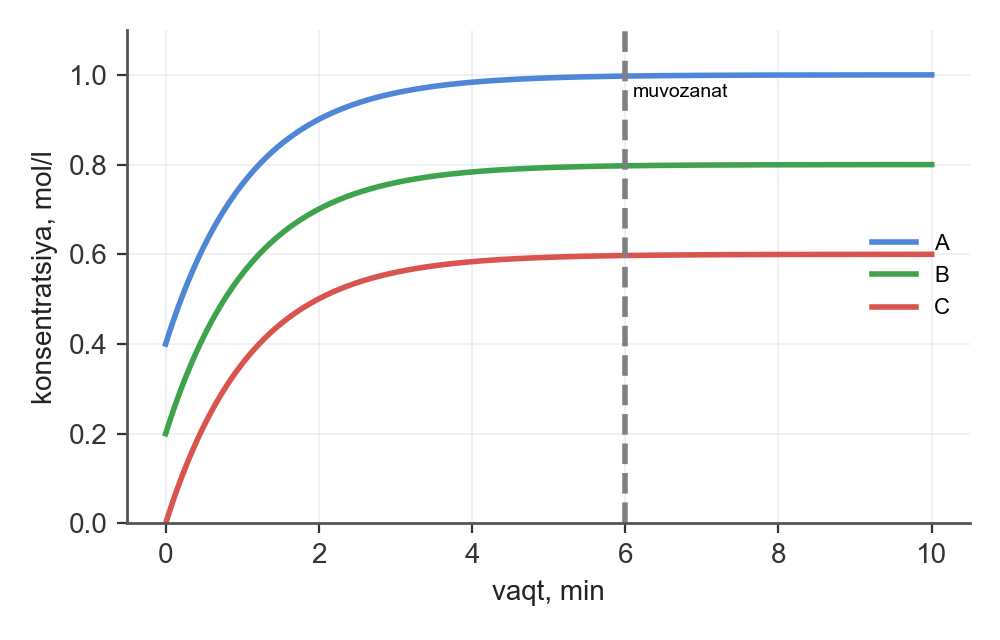
\includegraphics[width=0.86\linewidth]{rasmlar/gen/conc_v09_0.png}\end{center}
Grafikdan foydalanib, muvozanat \textbf{konstantasini (K) aniqlang.}

\noindent A)~\textsl{15} \hfill B)~\textsl{7,5} \hfill C)~\textsl{3,75} \hfill D)~\textsl{1}\par
\qsep
\noindent\qn{2.} Quyidagi zarrachalardan qaysilari neon atomi bilan izoelektron? 1) Al\textsuperscript{3+}; 2) Cl\textsuperscript{$-$}; 3) S\textsuperscript{2$-$}; 4) F\textsuperscript{$-$}

\noindent A)~\textsl{2, 3, 4} \hfill B)~\textsl{1, 2} \hfill C)~\textsl{1, 4} \hfill D)~\textsl{2, 4}\par
\qsep
\noindent\qn{3.} N\textsubscript{2} + 3H\textsubscript{2} $\rightleftarrows$ 2NH\textsubscript{3} reaksiyasi 2 l hajmli idishda o`tkazildi. Ma'lumotlar jadvalda berilgan:
\begin{center}
\renewcommand{\arraystretch}{1.15}
\fitbox{\begin{tabular}{|c|c|c|c|}\hline
\textbf{Modda} & \textbf{N\textsubscript{2}} & \textbf{H\textsubscript{2}} & \textbf{NH\textsubscript{3}} \\ \hline
Boshlang`ich, mol & 4 & 6 & 0 \\ \hline
Muvozanatda, mol & --- & --- & 2 \\ \hline
\end{tabular}}
\end{center}
N\textsubscript{2} ning necha foizi reaksiyaga \textbf{kirishganini aniqlang.}

\noindent A)~\textsl{12,5} \hfill B)~\textsl{25} \hfill C)~\textsl{37,5} \hfill D)~\textsl{75}\par
\qsep
\noindent\qn{4.} Quyidagi tuzlarning qaysilari suvli eritmasi ishqoriy muhitga ega? 1) K\textsubscript{3}PO\textsubscript{4}; 2) ZnCl\textsubscript{2}; 3) K\textsubscript{2}SO\textsubscript{4}; 4) NH\textsubscript{4}Cl

\noindent A)~\textsl{1} \hfill B)~\textsl{2, 3} \hfill C)~\textsl{3} \hfill D)~\textsl{3, 4}\par
\qsep
\noindent\qn{5.} Gazlar aralashmasi tarkibi jadvalda berilgan (n.sh.):
\begin{center}
\renewcommand{\arraystretch}{1.15}
\fitbox{\begin{tabular}{|c|c|}\hline
\textbf{Gaz} & \textbf{Hajmi, l} \\ \hline
He & 1 \\ \hline
N\textsubscript{2} & 1 \\ \hline
SO\textsubscript{2} & 2 \\ \hline
\end{tabular}}
\end{center}
Aralashmaning havoga nisbatan \textbf{zichligini aniqlang} (M(havo) = 29 g/mol).

\noindent A)~\textsl{2,76} \hfill B)~\textsl{0,69} \hfill C)~\textsl{40} \hfill D)~\textsl{1,38}\par
\qsep
\noindent\qn{6.} Reaksiya tezligining harorat koeffitsiyenti $\gamma$ = 4. 20 \textdegree{}C da reaksiya 32 minutda tugasa, 40 \textdegree{}C da necha sekundda tugaydi?

\noindent A)~\textsl{30720} \hfill B)~\textsl{480} \hfill C)~\textsl{2} \hfill D)~\textsl{120}\par
\qsep
\noindent\qn{7.} 1 M HCl eritmasining normal \textbf{konsentratsiyasini (n) aniqlang.}

\noindent A)~\textsl{2} \hfill B)~\textsl{0,5} \hfill C)~\textsl{1} \hfill D)~\textsl{1,5}\par
\qsep
\noindent\qn{8.} NaCl eritmasi inert elektrodlar yordamida 10 A tok kuchi bilan 965 s elektroliz qilindi. Anodda ajralgan Cl\textsubscript{2} hajmi (l, n.sh.) \textbf{ni toping.}

\noindent A)~\textsl{2,24} \hfill B)~\textsl{1,12} \hfill C)~\textsl{0,56} \hfill D)~\textsl{0,112}\par
\qsep
\noindent\qn{9.} H\textsubscript{2} + I\textsubscript{2} $\rightleftarrows$ 2HI reaksiyada muvozanat qaror topganda [H\textsubscript{2}] = 1, [I\textsubscript{2}] = 2, [HI] = 4 mol/l bo`ldi. I\textsubscript{2} ning boshlang`ich \textbf{konsentratsiyasini (mol/l) aniqlang.}

\noindent A)~\textsl{4} \hfill B)~\textsl{2} \hfill C)~\textsl{6} \hfill D)~\textsl{8}\par
\qsep
\noindent\qn{10.} Faqat oksidlovchi bo`la oladigan \textbf{ionlarni aniqlang}: 1) I\textsuperscript{$-$}; 2) Cl\textsuperscript{$-$}; 3) K\textsuperscript{+}; 4) Na\textsuperscript{+}

\noindent A)~\textsl{1} \hfill B)~\textsl{1, 2, 4} \hfill C)~\textsl{2, 4} \hfill D)~\textsl{3, 4}\par
\qsep
\noindent\qn{11.} CuCl\textsubscript{2} ning suvli eritmasi inert elektrodlar bilan elektroliz qilinganda qaysi moddalar ajraladi?

\noindent\begin{tabular}{@{}p{0.47\linewidth}@{}p{0.47\linewidth}@{}}
A)~\textsl{Cu va O\textsubscript{2}} & B)~\textsl{Cu va Cl\textsubscript{2}} \\
C)~\textsl{Zn, H\textsubscript{2} va O\textsubscript{2}} & D)~\textsl{Ag va O\textsubscript{2}} \\
\end{tabular}\par
\qsep
\noindent\qn{12.} 4,6 g Na va 3,55 g Cl\textsubscript{2} aralashtirilib, reaksiya o`tkazildi (2Na + Cl\textsubscript{2} $\to$ 2NaCl). Hosil bo`lgan NaCl \textbf{massasini (g) aniqlang.}

\noindent A)~\textsl{5,85} \hfill B)~\textsl{11,7} \hfill C)~\textsl{2,93} \hfill D)~\textsl{8,78}\par
\qsep
\noindent\qn{13.} 18,25 g HCl 500 g suvda eritildi. Eritmaning molyal \textbf{konsentratsiyasini (mol/kg) aniqlang.}

\noindent A)~\textsl{0,96} \hfill B)~\textsl{0} \hfill C)~\textsl{2} \hfill D)~\textsl{1}\par
\qsep
\noindent\qn{14.} Reaksiya tenglamasi: ZnO + 2HCl $\to$ ZnCl\textsubscript{2} + H\textsubscript{2}O. Reaksiyaga tarkibida 20\% aralashma bo`lgan 20,25 g namuna (asosiy modda ZnO) kirishdi. HCl \textbf{hajmini (l, n.sh.) hisoblang.}

\noindent A)~\textsl{2,24} \hfill B)~\textsl{17,92} \hfill C)~\textsl{8,96} \hfill D)~\textsl{4,48}\par
\qsep
\noindent\qn{15.} Mg(HCO\textsubscript{3})\textsubscript{2} $\to$ MgCO\textsubscript{3} + CO\textsubscript{2} + H\textsubscript{2}O reaksiyasida 146 g Mg(HCO\textsubscript{3})\textsubscript{2} ishtirok etdi. MgCO\textsubscript{3} \textbf{massasini (g) toping.}

\noindent A)~\textsl{168} \hfill B)~\textsl{42} \hfill C)~\textsl{84} \hfill D)~\textsl{126}\par
\qsep
\noindent\qn{16.} Reaksiya tenglamasi: N\textsubscript{2}O\textsubscript{5} + H\textsubscript{2}O $\to$ 2HNO\textsubscript{3}. Reaksiyaga tarkibida 10\% aralashma bo`lgan 12 g namuna (asosiy modda N\textsubscript{2}O\textsubscript{5}) kirishdi. HNO\textsubscript{3} \textbf{massasini (g) hisoblang.}

\noindent A)~\textsl{3,15} \hfill B)~\textsl{25,2} \hfill C)~\textsl{12,6} \hfill D)~\textsl{6,3}\par
\qsep
\noindent\qn{17.} P $\to$ ? $\to$ ? $\to$ ? o`zgarishlar zanjirida (reagentlar: O\textsubscript{2}, H\textsubscript{2}O, KOH) 3-bosqichda hosil bo`ladigan modda \textbf{formulasini toping.}

\noindent A)~\textsl{SO\textsubscript{2}} \hfill B)~\textsl{Na\textsubscript{2}O} \hfill C)~\textsl{K\textsubscript{3}PO\textsubscript{4}} \hfill D)~\textsl{NaOH}\par
\qsep
\noindent\qn{18.} NH\textsubscript{3} + H\textsubscript{3}PO\textsubscript{4} $\to$ NH\textsubscript{4}H\textsubscript{2}PO\textsubscript{4} jarayoni uchun 98 g H\textsubscript{3}PO\textsubscript{4} olingan (unum 60\%). NH\textsubscript{4}H\textsubscript{2}PO\textsubscript{4} \textbf{massasini (g) aniqlang.}

\noindent A)~\textsl{115} \hfill B)~\textsl{138} \hfill C)~\textsl{69} \hfill D)~\textsl{34,5}\par
\qsep
\noindent\qn{19.} NH\textsubscript{4}NO\textsubscript{3} qizdirilganda qanday moddalar hosil bo`ladi?

\noindent\begin{tabular}{@{}p{0.47\linewidth}@{}p{0.47\linewidth}@{}}
A)~\textsl{Ag, NO\textsubscript{2} va O\textsubscript{2}} & B)~\textsl{KNO\textsubscript{2} va O\textsubscript{2}} \\
C)~\textsl{CuO, NO\textsubscript{2} va O\textsubscript{2}} & D)~\textsl{N\textsubscript{2}O va H\textsubscript{2}O} \\
\end{tabular}\par
\qsep
\noindent\qn{20.} CH\textsubscript{4} + Cl\textsubscript{2} $\to$ CH\textsubscript{3}Cl + HCl jarayoni uchun 4,48 l (n.sh.) CH\textsubscript{4} olingan. CH\textsubscript{3}Cl \textbf{miqdorini (mol) aniqlang.}

\noindent A)~\textsl{0,4} \hfill B)~\textsl{0,1} \hfill C)~\textsl{0,3} \hfill D)~\textsl{0,2}\par
\qsep
\noindent\qn{21.} Alken, alkadiyen va alkinlar haqida qaysi fikrlar to`g`ri? 1) Alkinlar uchun umumiy formula CnH\textsubscript{2}n+2; 2) Asetilen Ag\textsubscript{2}O ning ammiakli eritmasi bilan cho`kma beradi (butin-2 beradi); 3) Etilen bromli suvni rangsizlantiradi; 4) Alkenlarda $\pi$-bog` yo`q

\noindent A)~\textsl{2, 3} \hfill B)~\textsl{3} \hfill C)~\textsl{1, 4} \hfill D)~\textsl{1, 3}\par
\qsep
\noindent\qn{22.} Rasmda siklik uglevodorodning tuzilish formulasi berilgan.
\begin{center}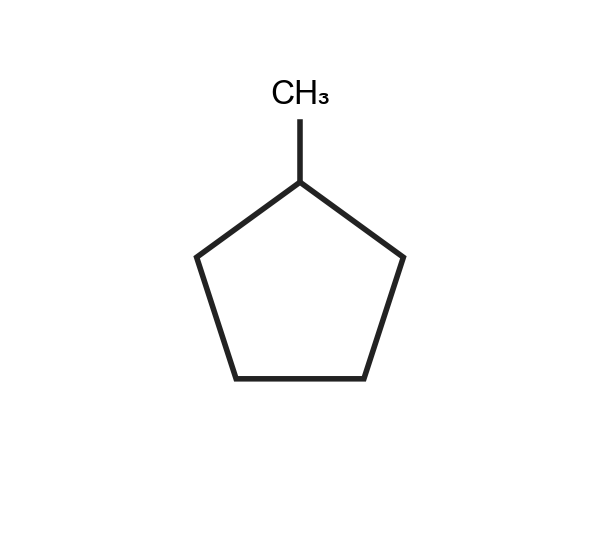
\includegraphics[width=0.86\linewidth]{rasmlar/gen/rn_873219.png}\end{center}
Birikmaning \textbf{nomini toping.}

\noindent\begin{tabular}{@{}p{0.47\linewidth}@{}p{0.47\linewidth}@{}}
A)~\textsl{1,2-dimetilsiklogeksan} & B)~\textsl{metilsiklopropan} \\
C)~\textsl{1,2-dimetilsiklopentan} & D)~\textsl{metilsiklopentan} \\
\end{tabular}\par
\qsep
\noindent\qn{23.} Spirt va fenollar haqida qaysi fikrlar to`g`ri? 1) Fenol FeCl\textsubscript{3} bilan binafsha rang beradi; 2) Glitserin Cu(OH)\textsubscript{2} bilan ko`k kompleks hosil qiladi; 3) Fenol Cu(OH)\textsubscript{2} ni eritib ko`k kompleks hosil qiladi; 4) Uchlamchi spirtlar oson oksidlanadi

\noindent A)~\textsl{4} \hfill B)~\textsl{1, 2} \hfill C)~\textsl{3} \hfill D)~\textsl{1, 2, 4}\par
\qsep
\noindent\qn{24.} 18 g glyukoza Ag\textsubscript{2}O ning ammiakli eritmasi bilan to`liq oksidlanganda hosil bo`lgan kumush \textbf{massasini (g) aniqlang.}

\noindent A)~\textsl{21,6} \hfill B)~\textsl{10,8} \hfill C)~\textsl{43,2} \hfill D)~\textsl{18}\par
\qsep
\noindent\qn{25.} Karbon kislotalar haqida qaysi fikrlar to`g`ri? 1) Sirka kislota karbonatlar bilan CO\textsubscript{2} ajratadi; 2) Sirka angidrid ikki molekula sirka kislotadan suv chiqib hosil bo`ladi; 3) Benzoy kislota Na\textsubscript{2}CO\textsubscript{3} bilan reaksiyaga kirishmaydi; 4) Olein kislota Br\textsubscript{2} ni biriktiradi

\noindent A)~\textsl{1, 2, 4} \hfill B)~\textsl{1, 3} \hfill C)~\textsl{2, 3, 4} \hfill D)~\textsl{2, 4}\par
\qsep
\noindent\qn{26.} Murakkab efirlar va yog`lar haqida qaysi fikrlar to`g`ri? 1) Suyuq yog`lar to`yinmagan kislotalardan hosil bo`lgan; 2) Yog`lar glitserin va yuqori yog` kislotalarning murakkab efirlari; 3) Efirlanish reaksiyasi qaytmas; 4) Sovun --- yuqori yog` kislotalarning natriyli tuzi

\noindent A)~\textsl{1, 4} \hfill B)~\textsl{1, 2, 4} \hfill C)~\textsl{1, 3, 4} \hfill D)~\textsl{1, 3}\par
\qsep
\noindent\qn{27.} Uglevodlar haqida qaysi fikrlar to`g`ri? 1) Kraxmal yod bilan ko`k rang beradi; 2) Selluloza $\beta$-glyukoza qoldiqlaridan iborat; 3) Glyukoza gidrolizlanadi; 4) Glyukoza "kumush ko`zgu" reaksiyasini beradi

\noindent A)~\textsl{1, 3, 4} \hfill B)~\textsl{2, 3} \hfill C)~\textsl{1, 2, 4} \hfill D)~\textsl{1, 2, 3}\par
\qsep
\noindent\qn{28.} 15 g glitsin HCl bilan reaksiyaga kirishganda hosil bo`lgan tuz \textbf{massasini (g) aniqlang.}

\noindent A)~\textsl{22,3} \hfill B)~\textsl{15} \hfill C)~\textsl{7,3} \hfill D)~\textsl{44,6}\par
\qsep
\noindent\qn{29.} 5,6 g C\textsubscript{2}H\textsubscript{4} dan quyidagi ikki bosqichda C\textsubscript{2}H\textsubscript{5}OH olinadi: 1) C\textsubscript{2}H\textsubscript{4} + HCl $\to$ C\textsubscript{2}H\textsubscript{5}Cl (unum 80\%); 2) C\textsubscript{2}H\textsubscript{5}Cl + KOH $\to$ C\textsubscript{2}H\textsubscript{5}OH + KCl (unum 75\%). Oxirgi mahsulot C\textsubscript{2}H\textsubscript{5}OH ning \textbf{massasini (g) toping.}

\noindent A)~\textsl{6,9} \hfill B)~\textsl{5,52} \hfill C)~\textsl{7,36} \hfill D)~\textsl{9,2}\par
\qsep
\noindent\qn{30.} Rasmda tasvirlangan usul bilan qaysi aralashmani ajratish mumkin?
\begin{center}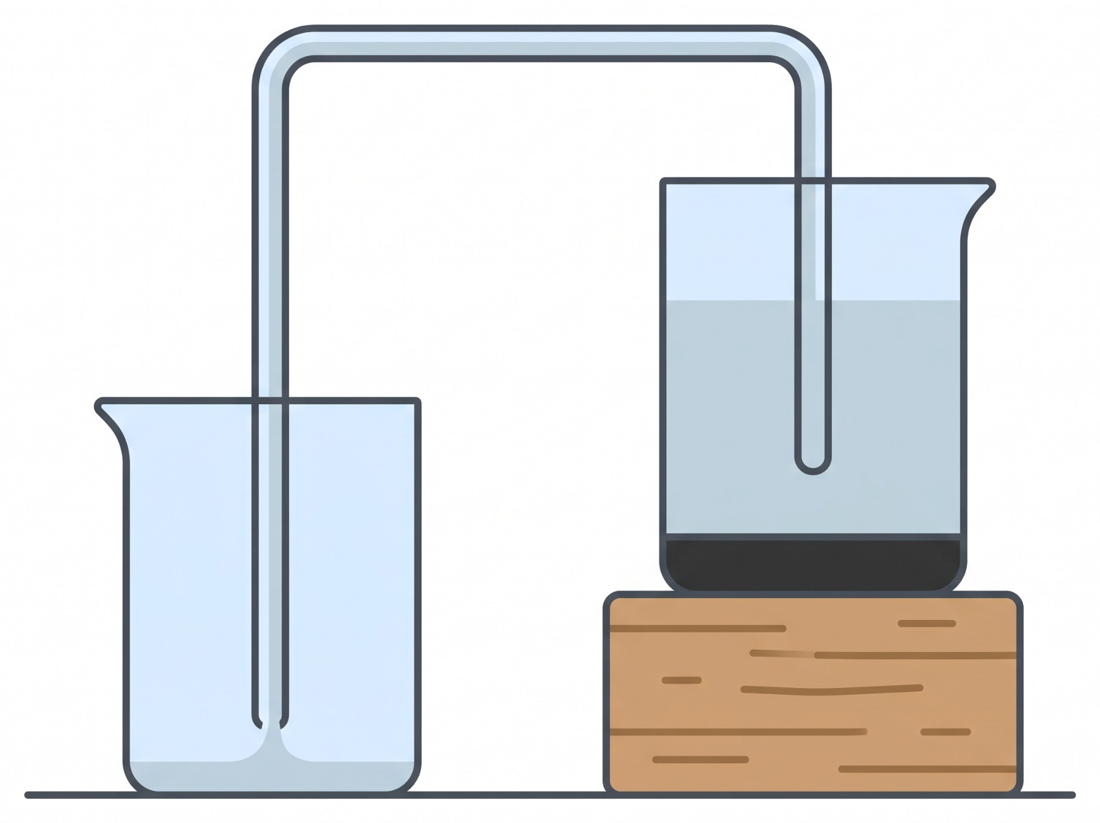
\includegraphics[width=0.86\linewidth]{rasmlar/darslik/d_tindirish.png}\end{center}
\noindent A)~\textsl{loyqa suv (suv va qum zarrachalari)}\par
\noindent B)~\textsl{suv va etanol}\par
\noindent C)~\textsl{suv va kerosin}\par
\noindent D)~\textsl{osh tuzi eritmasi}\par
\qsep
\noindent\qn{31.} Quyidagi aralashmani ajratish uchun qaysi usul mos: suv va etanol aralashmasi?
\noindent A)~\textsl{distillash (fraksiyalab haydash)}\par
\noindent B)~\textsl{ajratgich voronka}\par
\noindent C)~\textsl{bug`latish}\par
\noindent D)~\textsl{magnit yordamida ajratish (temir tortiladi)}\par
\qsep
\noindent\qn{32.} Eritmaga BaCl\textsubscript{2} qo`shilganda oq cho`kma (BaSO\textsubscript{4}), HCl da erimaydi kuzatildi. Eritmada qaysi ion bor?

\noindent\begin{tabular}{@{}p{0.47\linewidth}@{}p{0.47\linewidth}@{}}
A)~\textsl{NH\textsubscript{4}\textsuperscript{+}} & B)~\textsl{Br\textsuperscript{$-$}} \\
C)~\textsl{CO\textsubscript{3}\textsuperscript{2$-$}} & D)~\textsl{SO\textsubscript{4}\textsuperscript{2$-$}   ---} \\
\end{tabular}\par
\qsep
\end{multicols}
\medskip
\noindent\setlength{\fboxsep}{0pt}\fbox{\begin{tabular}{p{0.74\linewidth}|p{0.2\linewidth}}
\parbox[t]{0.72\linewidth}{\vspace{3pt}\textbf{Topshiriqlar (33--35) va javob variant (A--F)larini o`zaro to`g`ri moslashtiring.} NaBr va NaCl dan iborat 16,15 g aralashma suvda eritilib, mo`l AgNO\textsubscript{3} eritmasi qo`shildi; hosil bo`lgan cho`kmalarning umumiy massasi 33,15 g.
\vspace{3pt}} & \parbox[t]{0.19\linewidth}{\vspace{3pt}A~\textsl{5,15}\\[3pt]
B~\textsl{8,5}\\[3pt]
C~\textsl{10,3}\\[3pt]
D~\textsl{17}\\[3pt]
E~\textsl{340}\\[3pt]
F~\textsl{510}}\\ \hline
\parbox[t]{0.72\linewidth}{\vspace{2pt}\textbf{33. Aralashmadagi NaBr massasini (g) aniqlang.}\vspace{2pt}} & \\ \hline
\parbox[t]{0.72\linewidth}{\vspace{2pt}\textbf{34. Sarflangan 10\% li AgNO\textsubscript{3} eritmasining massasini (g) aniqlang (M(AgNO\textsubscript{3}) = 170 g/mol).}\vspace{2pt}} & \\ \hline
\parbox[t]{0.72\linewidth}{\vspace{2pt}\textbf{35. Eritmada hosil bo`lgan nitratlarning umumiy massasini (g) aniqlang.}\vspace{2pt}} & 
\end{tabular}}
\par\bigskip
\noindent\qn{36.} Cu + HNO\textsubscript{3} $\to$ Cu(NO\textsubscript{3})\textsubscript{2} + NO + H\textsubscript{2}O reaksiya tenglamasini tenglang va barcha koeffitsiyentlar \textbf{yig`indisini aniqlang.}
\javob\qsep
\noindent\qn{37.} Reaksiya 30 \textdegree{}C da 72 minutda tugaydi. $\gamma$ = 2. Harorat 20 \textdegree{}C ga oshirilib, reagentlardan birining konsentratsiyasi 2 marta oshirildi (reaksiya shu modda bo`yicha 1-tartibli). Reaksiya necha minutda tugaydi?
\javob\qsep
\noindent\qn{38.} 37,6 g Cu(NO\textsubscript{3})\textsubscript{2} qizdirilganda qisman parchalandi, qattiq qoldiq massasi 26,8 g bo`ldi. Ajralgan gazlar (n.sh.) \textbf{hajmini (l) hisoblang.}
\javob\qsep
\noindent\qn{39.} Etilen va asetilendan iborat 4,48 l (n.sh.) aralashma bromli suvdan o`tkazilganda 40 g brom yutildi. Aralashmadagi asetilenning \textbf{hajmini (l, n.sh.) toping.}
\javob\qsep
\noindent\qn{40.} Polistirol polimerining (polimerlanish darajasi 2000) 416 g namunasini olish uchun polimerlanish unumi 80\% bo`lganda qancha monomer (C\textsubscript{8}H\textsubscript{8}) kerak (g)?
\javob\qsep
\par\bigskip\begin{center}\textbf{\fontsize{13}{15}\selectfont YOZMA ISH}\end{center}
\noindent\qn{41.} \textbf{Topshiriqni bajarish jarayonida barcha reaksiya tenglamalarini yozing. Miqdoriy va arifmetik hisoblashlarni (unga asos bo`lgan usul yoki formulani ko`rsatgan holda) uzviy ketma-ketlikda bajaring.}\par\smallskip
Elementar 2SO\textsubscript{2} + O\textsubscript{2} $\to$ 2SO\textsubscript{3} reaksiyasi 30 \textdegree{}C da 162 minutda tugaydi. Reaksiyaning temperatura koeffitsiyenti $\gamma$ = 3. Boshlang`ich konsentratsiyalar [SO\textsubscript{2}] = [O\textsubscript{2}] = 0,2 mol/l bo`lganda boshlang`ich tezlik 1$\cdot$10\textsuperscript{$-$3} mol/(l$\cdot$min) ga teng.\par
\noindent 1)\ Reaksiya tezligi konstantasini (k) hisoblang va kinetik tenglamani yozing.\par
\noindent 2)\ Harorat 40 \textdegree{}C ga oshirilganda reaksiya tezligi necha marta ortadi?\par
\noindent 3)\ Harorat 40 \textdegree{}C ga oshirilganda reaksiya necha minutda tugaydi?\par
\noindent 4)\ Idish hajmi 2 marta kamaytirilsa, 30 \textdegree{}C da tezlik necha marta o`zgaradi? Idish hajmi 3 marta oshirilsa tezlik necha marta kamayadi?\par
\noindent 5)\ SO\textsubscript{2} ning konsentratsiyasini 3 marta oshirib, O\textsubscript{2} niki o`zgarmasa, tezlik necha marta o`zgaradi? Shuningdek harorat 30 \textdegree{}C dan 10 \textdegree{}C gacha pasaytirilsa tezlik necha marta kamayadi?\par
\diqqat{Mazkur topshiriq kengaytirilgan javobni talab etib, uning yechilish usuli va shu usul asosidagi barcha hisoblash amallari javoblar varaqasida aks etishi lozim.}\qsep
\noindent\qn{42.} Quyidagi o`zgarishlar zanjirida \textit{X}, \textit{Y}, \textit{Z} noma'lum organik moddalar:\par
\[\setlength{\fboxsep}{0pt}\text{C\textsubscript{2}H\textsubscript{5}OH}\xrightarrow{\text{CuO, t\textdegree{}}}\text{\textit{X}}\xrightarrow{\text{Ag\textsubscript{2}O, NH\textsubscript{3}}}\text{\textit{Y}}\xrightarrow{\text{Cl\textsubscript{2}, P}}\text{\textit{Z}}\xrightarrow{\text{NH\textsubscript{3}}}\text{NH\textsubscript{2}CH\textsubscript{2}COOH}\]
\noindent 1)\ C\textsubscript{2}H\textsubscript{5}OH $\to$ \textit{X} : reaksiya tenglamasini yozing; hosil bo`lgan moddani nomlang.\par
\noindent 2)\ \textit{X} $\to$ \textit{Y} : reaksiya tenglamasini yozing; hosil bo`lgan moddani nomlang.\par
\noindent 3)\ \textit{Y} $\to$ \textit{Z} : reaksiya tenglamasini yozing; hosil bo`lgan moddani nomlang.\par
\noindent 4)\ \textit{Z} $\to$ NH\textsubscript{2}CH\textsubscript{2}COOH : reaksiya tenglamasini yozing; hosil bo`lgan moddani nomlang.\par
\diqqat{Mazkur topshiriq kengaytirilgan javobni talab etib, uning yechilish usuli va shu usul asosidagi barcha hisoblash amallari javoblar varaqasida aks etishi lozim.}\qsep
\noindent\qn{43.} \textbf{Topshiriqni bajarish jarayonida barcha reaksiya tenglamalarini yozing. Miqdoriy va arifmetik hisoblashlarni (unga asos bo`lgan usul yoki formulani ko`rsatgan holda) uzviy ketma-ketlikda bajaring.}\par\smallskip
12,4 g qizil fosfor mo`l kislorodda yondirildi, hosil bo`lgan oksid suvda to`liq eritildi (ortofosfat kislota). Eritmaga 0,8 mol NaOH qo`shildi.\par
\noindent 1)\ Reaksiya tenglamalarini yozing. Hosil bo`lgan P\textsubscript{2}O\textsubscript{5} massasini (g) hisoblang.\par
\noindent 2)\ Hosil bo`lgan H\textsubscript{3}PO\textsubscript{4} massasini (g) toping. Kislotada fosforning massa ulushini (\%) ham hisoblang.\par
\noindent 3)\ Eritmada qanday tuz hosil bo`lganini aniqlang va uning massasini (g) hisoblang.\par
\noindent 4)\ Hosil bo`lgan eritmani to`liq neytrallash uchun yana qancha NaOH (g) kerak (Na\textsubscript{2}HPO\textsubscript{4} $\to$ Na\textsubscript{3}PO\textsubscript{4})?\par
\noindent 5)\ Hosil bo`lgan tuzning 10\% li eritmasi massasini (g) hisoblang.\par
\diqqat{Mazkur topshiriq kengaytirilgan javobni talab etib, uning yechilish usuli va shu usul asosidagi barcha hisoblash amallari javoblar varaqasida aks etishi lozim.}\qsep
\newpage
\renewcommand{\curvar}{10-variant}
\thispagestyle{first}
\noindent\textit{Davriy jadvaldan foydalanish mumkin.}
\par\smallskip
\begin{multicols}{2}
\noindent\qn{1.} PCl\textsubscript{5} $\rightleftarrows$ PCl\textsubscript{3} + Cl\textsubscript{2} reaksiyasi 1 l hajmli idishda o`tkazildi. Ma'lumotlar jadvalda berilgan:
\begin{center}
\renewcommand{\arraystretch}{1.15}
\fitbox{\begin{tabular}{|c|c|c|}\hline
\textbf{Modda} & \textbf{PCl\textsubscript{5}} & \textbf{PCl\textsubscript{3}} \\ \hline
Boshlang`ich, mol & 6 & 0 \\ \hline
Muvozanatda, mol & --- & 0,5 \\ \hline
\end{tabular}}
\end{center}
Muvozanat \textbf{konstantasini (K) hisoblang.}

\noindent A)~\textsl{0,091} \hfill B)~\textsl{0,045} \hfill C)~\textsl{0,023} \hfill D)~\textsl{22}\par
\qsep
\noindent\qn{2.} 10 l SO\textsubscript{2} va 10 l O\textsubscript{2} aralashmasi reaksiyaga kirishdi (2SO\textsubscript{2} + O\textsubscript{2} $\to$ 2SO\textsubscript{3}, hamma moddalar bir xil sharoitda gaz holida). Reaksiyadan keyingi gaz aralashmasining \textbf{hajmini (l) aniqlang.}

\noindent A)~\textsl{15} \hfill B)~\textsl{20} \hfill C)~\textsl{10} \hfill D)~\textsl{5}\par
\qsep
\noindent\qn{3.} KClO\textsubscript{3} tarkibida Cl ning oksidlanish \textbf{darajasini aniqlang.}

\noindent A)~\textsl{+6} \hfill B)~\textsl{+7} \hfill C)~\textsl{+5} \hfill D)~\textsl{$-$2}\par
\qsep
\noindent\qn{4.} Azot atomining p- va d- pog`onachalaridagi elektronlardan nechtasining magnit kvant soni m\_l = 1 ga teng? (\textit{Z} = 7)

\noindent A)~\textsl{2} \hfill B)~\textsl{1} \hfill C)~\textsl{4} \hfill D)~\textsl{3}\par
\qsep
\noindent\qn{5.} 1 mol AlCl\textsubscript{3} va 3 mol Ba(OH)\textsubscript{2} suvda eritilib, eritma hajmi 2 l ga yetkazildi. Eritmadagi barcha ionlarning umumiy molyar \textbf{konsentratsiyasini (mol/l) aniqlang} (kuchli elektrolitlar to`liq dissotsilanadi).

\noindent A)~\textsl{2} \hfill B)~\textsl{13} \hfill C)~\textsl{3,25} \hfill D)~\textsl{6,5}\par
\qsep
\noindent\qn{6.} 16,8 g CaO va 8,1 g H\textsubscript{2}O aralashtirilib, reaksiya o`tkazildi (CaO + H\textsubscript{2}O $\to$ Ca(OH)\textsubscript{2}). Hosil bo`lgan Ca(OH)\textsubscript{2} \textbf{massasini (g) aniqlang.}

\noindent A)~\textsl{33,3} \hfill B)~\textsl{44,4} \hfill C)~\textsl{22,2} \hfill D)~\textsl{11,1}\par
\qsep
\noindent\qn{7.} N\textsubscript{2} + 3H\textsubscript{2} $\rightleftarrows$ 2NH\textsubscript{3} reaksiyada muvozanat qaror topganda [N\textsubscript{2}] = 1, [H\textsubscript{2}] = 1, [NH\textsubscript{3}] = 4 mol/l bo`ldi. N\textsubscript{2} ning boshlang`ich \textbf{konsentratsiyasini (mol/l) aniqlang.}

\noindent A)~\textsl{3} \hfill B)~\textsl{1} \hfill C)~\textsl{5} \hfill D)~\textsl{6}\par
\qsep
\noindent\qn{8.} Gazlar aralashmasi tarkibi jadvalda berilgan (n.sh.):
\begin{center}
\renewcommand{\arraystretch}{1.15}
\fitbox{\begin{tabular}{|c|c|}\hline
\textbf{Gaz} & \textbf{Hajmi, l} \\ \hline
NH\textsubscript{3} & 1 \\ \hline
SO\textsubscript{2} & 3 \\ \hline
O\textsubscript{2} & 3 \\ \hline
\end{tabular}}
\end{center}
Aralashmaning havoga nisbatan \textbf{zichligini aniqlang} (M(havo) = 29 g/mol).

\noindent A)~\textsl{3} \hfill B)~\textsl{1,5} \hfill C)~\textsl{0,75} \hfill D)~\textsl{43,57}\par
\qsep
\noindent\qn{9.} 300 g 10\% li Na\textsubscript{2}SO\textsubscript{4} eritmasiga 25 g shu tuzning o`zi qo`shilib eritildi. Hosil bo`lgan eritmaning massa \textbf{ulushini (\%) aniqlang.}

\noindent A)~\textsl{16,92} \hfill B)~\textsl{18,33} \hfill C)~\textsl{9,17} \hfill D)~\textsl{13,54}\par
\qsep
\noindent\qn{10.} Azot (\textit{Z} = 7) atomining tashqi energetik pog`onasidagi elektronlar \textbf{sonini aniqlang.}

\noindent A)~\textsl{6} \hfill B)~\textsl{4} \hfill C)~\textsl{5} \hfill D)~\textsl{7}\par
\qsep
\noindent\qn{11.} Quyidagi zarrachalardan qaysilari argon atomi bilan izoelektron? 1) Na\textsuperscript{+}; 2) Cl\textsuperscript{$-$}; 3) Ca\textsuperscript{2+}; 4) K\textsuperscript{+}

\noindent A)~\textsl{2, 4} \hfill B)~\textsl{1, 3, 4} \hfill C)~\textsl{2, 3, 4} \hfill D)~\textsl{1, 4}\par
\qsep
\noindent\qn{12.} KNO\textsubscript{3} va NaCl eruvchanligining haroratga bog`liqligi grafikda berilgan.
\begin{center}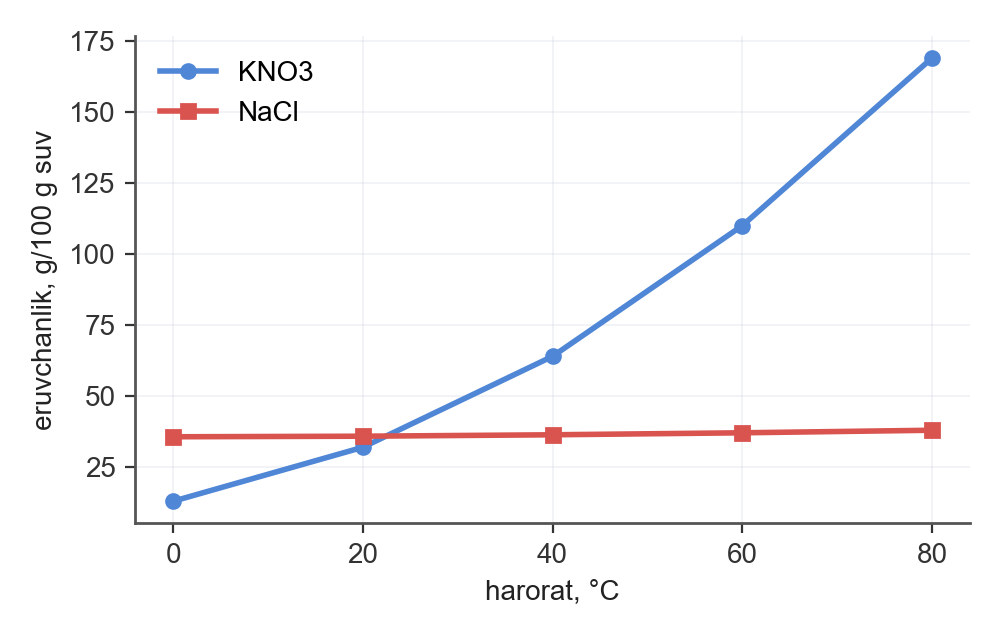
\includegraphics[width=0.86\linewidth]{rasmlar/gen/s2_v10_0.png}\end{center}
60 \textdegree{}C da qaysi tuzning eruvchanligi katta?

\noindent A)~\textsl{NaCl} \hfill B)~\textsl{KCl} \hfill C)~\textsl{NH\textsubscript{4}Cl} \hfill D)~\textsl{KNO\textsubscript{3}}\par
\qsep
\noindent\qn{13.} 16,1 g Na\textsubscript{2}SO\textsubscript{4}$\cdot$10H\textsubscript{2}O 100 g suvda eritildi. Eritmadagi tuzning massa \textbf{ulushini (\%) aniqlang.}

\noindent A)~\textsl{7,1} \hfill B)~\textsl{13,87} \hfill C)~\textsl{12,23} \hfill D)~\textsl{6,12}\par
\qsep
\noindent\qn{14.} Quyidagi tuzlardan qaysilari asosli tuz? 1) K\textsubscript{2}SO\textsubscript{4}; 2) (CuOH)\textsubscript{2}CO\textsubscript{3}; 3) CaCO\textsubscript{3}; 4) KAl(SO\textsubscript{4})\textsubscript{2}

\noindent A)~\textsl{2, 4} \hfill B)~\textsl{2} \hfill C)~\textsl{2, 3} \hfill D)~\textsl{4}\par
\qsep
\noindent\qn{15.} CaCO\textsubscript{3} $\to$ CaO + CO\textsubscript{2} jarayoni uchun 50 g CaCO\textsubscript{3} olingan (unum 90\%). CaO \textbf{massasini (g) aniqlang.}

\noindent A)~\textsl{28} \hfill B)~\textsl{50,4} \hfill C)~\textsl{25,2} \hfill D)~\textsl{12,6}\par
\qsep
\noindent\qn{16.} Nodir gazlar haqida qaysi fikrlar to`g`ri? 1) Argon elektr lampalarida ishlatiladi; 2) Nodir gazlar odatiy sharoitda ko`p atomli molekulalar hosil qiladi; 3) Nodir gazlar kimyoviy jihatdan juda faol; 4) Neon reklama naylarida ishlatiladi

\noindent A)~\textsl{1, 2, 3} \hfill B)~\textsl{2, 3} \hfill C)~\textsl{3, 4} \hfill D)~\textsl{1, 4}\par
\qsep
\noindent\qn{17.} 2NaNO\textsubscript{3} $\to$ 2NaNO\textsubscript{2} + O\textsubscript{2} reaksiyasida tarkibida 60\% aralashma bo`lgan 42,5 g namuna (asosiy modda NaNO\textsubscript{3}) ishtirok etdi. NaNO\textsubscript{2} \textbf{massasini (g) toping.}

\noindent A)~\textsl{27,6} \hfill B)~\textsl{6,9} \hfill C)~\textsl{13,8} \hfill D)~\textsl{20,7}\par
\qsep
\noindent\qn{18.} 60 g FeS\textsubscript{2} yondirilib, hosil bo`lgan SO\textsubscript{2} dan H\textsubscript{2}SO\textsubscript{4} olindi (jami unum 100\%). Sulfat kislota \textbf{massasini (g) aniqlang.}

\noindent A)~\textsl{98} \hfill B)~\textsl{49} \hfill C)~\textsl{196} \hfill D)~\textsl{147}\par
\qsep
\noindent\qn{19.} KNO\textsubscript{3} qizdirilganda qanday moddalar hosil bo`ladi?

\noindent\begin{tabular}{@{}p{0.47\linewidth}@{}p{0.47\linewidth}@{}}
A)~\textsl{N\textsubscript{2}O va H\textsubscript{2}O} & B)~\textsl{Ag, NO\textsubscript{2} va O\textsubscript{2}} \\
C)~\textsl{KNO\textsubscript{2} va O\textsubscript{2}} & D)~\textsl{CuO, NO\textsubscript{2} va O\textsubscript{2}} \\
\end{tabular}\par
\qsep
\noindent\qn{20.} Rasmda uchta uglevodorodning tuzilish formulasi berilgan.
\begin{center}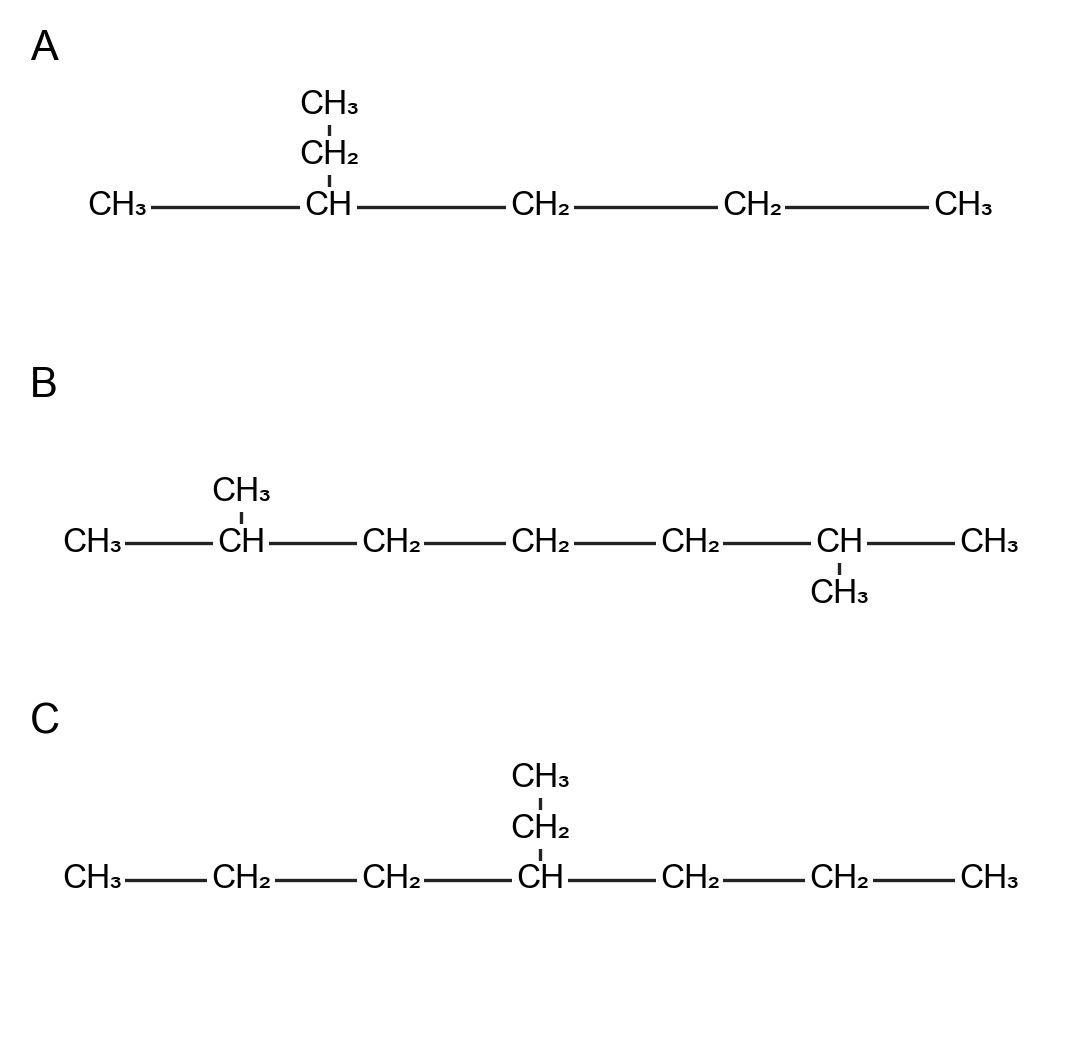
\includegraphics[width=0.86\linewidth]{rasmlar/gen/is_479186.png}\end{center}
Qaysi juftlik o`zaro izomerlar hisoblanadi?

\noindent A)~\textsl{A va B} \hfill B)~\textsl{A va C} \hfill C)~\textsl{A, B va C} \hfill D)~\textsl{B va C}\par
\qsep
\noindent\qn{21.} CH\textsubscript{2}=CH--CH\textsubscript{2}--CH\textsubscript{3} birikmaning sistematik nomi qaysi qatorda to`g`ri keltirilgan?

\noindent A)~\textsl{buten-2} \hfill B)~\textsl{buten-1} \hfill C)~\textsl{1-butin} \hfill D)~\textsl{butan}\par
\qsep
\noindent\qn{22.} Arenlar, neft va tabiiy gaz haqida qaysi fikrlar to`g`ri? 1) Benzol bromli suvni rangsizlantirmaydi; 2) Tabiiy gazning asosiy qismi propan; 3) Neft fraksiyalaridan gazolin 150 \textdegree{}C gacha haydaladi; 4) Benzoldan nitrobenzol nitrolash bilan olinadi

\noindent A)~\textsl{3, 4} \hfill B)~\textsl{1, 2} \hfill C)~\textsl{1, 3, 4} \hfill D)~\textsl{2, 3, 4}\par
\qsep
\noindent\qn{23.} C\textsubscript{2}H\textsubscript{5}OH + CuO (t) reaksiyasi natijasida qaysi organik modda hosil bo`ladi?

\noindent\begin{tabular}{@{}p{0.47\linewidth}@{}p{0.47\linewidth}@{}}
A)~\textsl{sirka aldegid} & B)~\textsl{etilen} \\
C)~\textsl{etanol} & D)~\textsl{asetilen} \\
\end{tabular}\par
\qsep
\noindent\qn{24.} Aldegid va ketonlar haqida qaysi fikrlar to`g`ri? 1) Formalin --- formaldegidning 40\% li eritmasi; 2) Aldegidlar qaytarilganda ikkilamchi spirt hosil bo`ladi; 3) Sirka aldegid Kucherov reaksiyasi bilan olinadi; 4) Ketonlar kuchsiz oksidlovchilar bilan oksidlanmaydi

\noindent A)~\textsl{2, 3, 4} \hfill B)~\textsl{1, 3} \hfill C)~\textsl{1, 4} \hfill D)~\textsl{1, 3, 4}\par
\qsep
\noindent\qn{25.} CH\textsubscript{3}COOH + C\textsubscript{2}H\textsubscript{5}OH $\to$ CH\textsubscript{3}COOC\textsubscript{2}H\textsubscript{5} + H\textsubscript{2}O jarayoni uchun 46 g C\textsubscript{2}H\textsubscript{5}OH olingan (unum 75\%). CH\textsubscript{3}COOC\textsubscript{2}H\textsubscript{5} \textbf{massasini (g) aniqlang.}

\noindent A)~\textsl{88} \hfill B)~\textsl{132} \hfill C)~\textsl{33} \hfill D)~\textsl{66}\par
\qsep
\noindent\qn{26.} Murakkab efirlar va yog`lar haqida qaysi fikrlar to`g`ri? 1) Murakkab efirlarning gidrolizi ishqoriy muhitda qaytmas; 2) Suyuq yog`larni gidrogenlab qattiq yog` olinadi; 3) Sovun --- yuqori yog` kislotalarning natriyli tuzi; 4) Suyuq yog`lar to`yinmagan kislotalardan hosil bo`lgan

\noindent\begin{tabular}{@{}p{0.47\linewidth}@{}p{0.47\linewidth}@{}}
A)~\textsl{1, 2, 3, 4} & B)~\textsl{1, 2, 3} \\
C)~\textsl{1, 3, 4} & D)~\textsl{1, 2, 4} \\
\end{tabular}\par
\qsep
\noindent\qn{27.} 68,4 g saxaroza gidrolizlanganda necha gramm glyukoza hosil bo`ladi?

\noindent A)~\textsl{36} \hfill B)~\textsl{68,4} \hfill C)~\textsl{72} \hfill D)~\textsl{18}\par
\qsep
\noindent\qn{28.} 26,7 g alanin HCl bilan reaksiyaga kirishganda hosil bo`lgan tuz \textbf{massasini (g) aniqlang.}

\noindent A)~\textsl{26,7} \hfill B)~\textsl{10,95} \hfill C)~\textsl{75,3} \hfill D)~\textsl{37,65}\par
\qsep
\noindent\qn{29.} C\textsubscript{2}H\textsubscript{4} + Cl\textsubscript{2} $\to$ C\textsubscript{2}H\textsubscript{4}Cl\textsubscript{2} reaksiyasida 4,48 l (n.sh.) Cl\textsubscript{2} ishtirok etdi. C\textsubscript{2}H\textsubscript{4}Cl\textsubscript{2} \textbf{massasini (g) toping.}

\noindent A)~\textsl{39,6} \hfill B)~\textsl{19,8} \hfill C)~\textsl{9,9} \hfill D)~\textsl{29,7}\par
\qsep
\noindent\qn{30.} Rasmdagi asbobda 6,5 g rux mo`l xlorid kislota bilan reaksiyaga kirishdi (Zn + 2HCl $\to$ ZnCl\textsubscript{2} + H\textsubscript{2}). Ajralgan vodorodning \textbf{hajmini (l, n.sh.) aniqlang.}
\begin{center}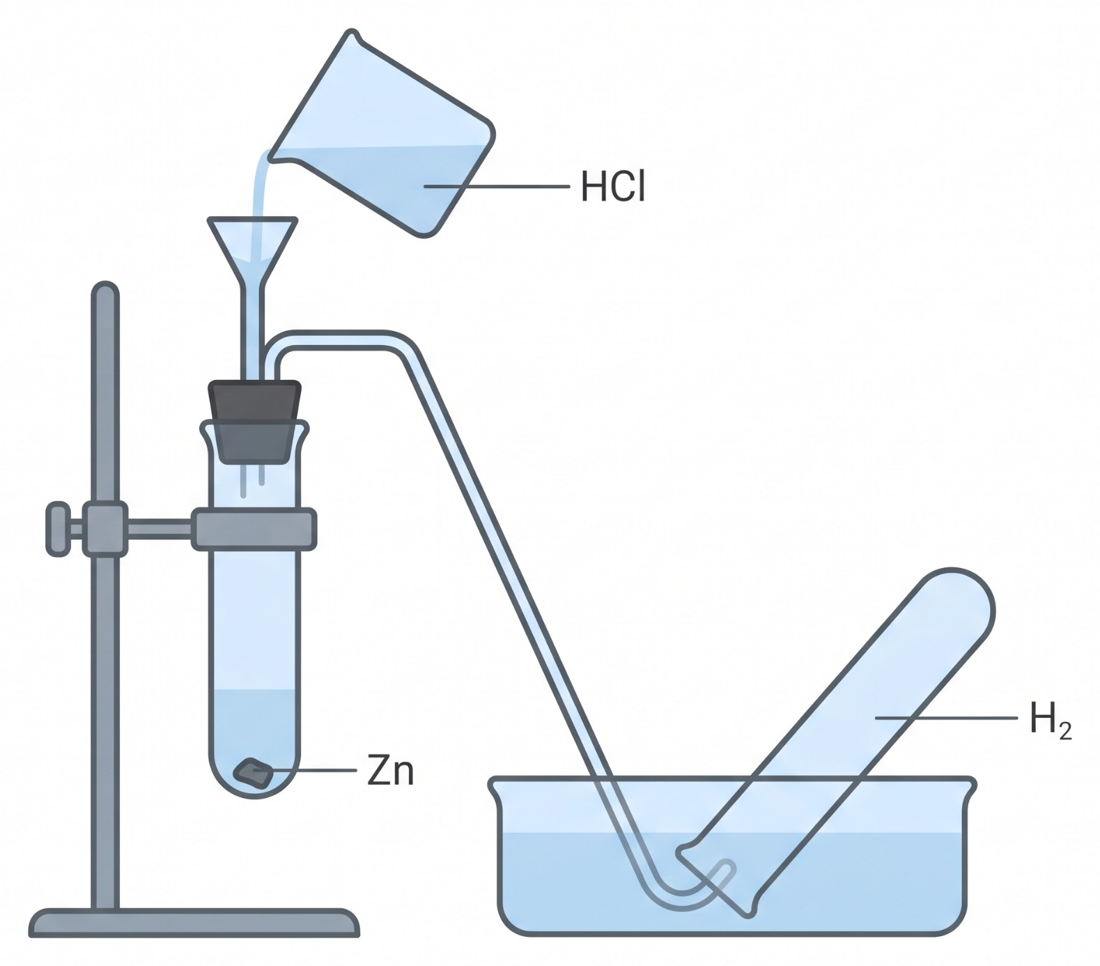
\includegraphics[width=0.86\linewidth]{rasmlar/darslik/d_vodorod.png}\end{center}

\noindent A)~\textsl{4,48} \hfill B)~\textsl{2,24} \hfill C)~\textsl{1,12} \hfill D)~\textsl{0,1}\par
\qsep
\noindent\qn{31.} 200 g 30\% li va 100 g 50\% li Na\textsubscript{2}SO\textsubscript{4} eritmalari aralashtirildi. Yangi eritmaning massa \textbf{ulushini (\%) toping.}

\noindent A)~\textsl{36,67} \hfill B)~\textsl{40} \hfill C)~\textsl{80} \hfill D)~\textsl{33}\par
\qsep
\noindent\qn{32.} Kimyoviy laboratoriyada o`lchov silindri nima uchun ishlatiladi?
\noindent A)~\textsl{eritmaning kichik hajmlarini o`lchab olish}\par
\noindent B)~\textsl{suyuqlik hajmini o`lchash}\par
\noindent C)~\textsl{eritmalarni bug`latish}\par
\noindent D)~\textsl{titrlashda reagent hajmini aniq o`lchash   ---}\par
\qsep
\end{multicols}
\medskip
\noindent\setlength{\fboxsep}{0pt}\fbox{\begin{tabular}{p{0.74\linewidth}|p{0.2\linewidth}}
\parbox[t]{0.72\linewidth}{\vspace{3pt}\textbf{Topshiriqlar (33--35) va javob variant (A--F)larini o`zaro to`g`ri moslashtiring.} Etanol va fenoldan iborat 28 g aralashma natriy bilan to`liq reaksiyaga kirishganda 4,48 l (n.sh.) vodorod ajraldi. Xuddi shu massadagi aralashma NaOH eritmasi bilan (faqat fenol) va bromli suv bilan (faqat fenol) ham reaksiyaga kirishadi.
\vspace{3pt}} & \parbox[t]{0.19\linewidth}{\vspace{3pt}A~\textsl{67,14}\\[3pt]
B~\textsl{47,66}\\[3pt]
C~\textsl{8}\\[3pt]
D~\textsl{119,16}\\[3pt]
E~\textsl{59,58}\\[3pt]
F~\textsl{12}}\\ \hline
\parbox[t]{0.72\linewidth}{\vspace{2pt}\textbf{33. Aralashmadagi fenol massa ulushini (\%) aniqlang.}\vspace{2pt}} & \\ \hline
\parbox[t]{0.72\linewidth}{\vspace{2pt}\textbf{34. Fenolni to`liq neytrallash uchun zarur NaOH massasini (g) aniqlang.}\vspace{2pt}} & \\ \hline
\parbox[t]{0.72\linewidth}{\vspace{2pt}\textbf{35. Mo`l bromli suv bilan reaksiyada hosil bo`lgan tribromfenol massasini (g) aniqlang (reaksiya unumi 90\%).}\vspace{2pt}} & 
\end{tabular}}
\par\bigskip
\noindent\qn{36.} Cu + HNO\textsubscript{3} $\to$ Cu(NO\textsubscript{3})\textsubscript{2} + NO\textsubscript{2} + H\textsubscript{2}O reaksiya tenglamasini tenglang va barcha koeffitsiyentlar \textbf{yig`indisini aniqlang.}
\javob\qsep
\noindent\qn{37.} Ketma-ket ulangan ikkita elektrolizyordan (CuSO\textsubscript{4} va AgNO\textsubscript{3} eritmalari, inert elektrodlar) tok o`tkazildi. Birinchi elektrolizyor katodida 12,8 g mis ajraldi. Ikkala elektrolizyor anodlarida ajralgan kislorodning umumiy \textbf{hajmini (l, n.sh.) toping} (anodda ikkalasida ham O\textsubscript{2} ajraladi).
\javob\qsep
\noindent\qn{38.} Alyuminiy va kalsiy dan iborat 13,4 g aralashma mo`l xlorid kislotada eritilganda 11,2 l (n.sh.) vodorod ajraldi. Aralashmadagi alyuminiyning massa \textbf{ulushini (\%) aniqlang.}
\javob\qsep
\noindent\qn{39.} 61,5 g nitrobenzoldan anilin olishda unum 75\% bo`lsa, mahsulot \textbf{massasini (g) aniqlang.}
\javob\qsep
\noindent\qn{40.} 22,2 g propion kislota va 9,6 g metanol dan 75\% unum bilan murakkab efir olindi. Efir \textbf{massasini (g) toping.}
\javob\qsep
\par\bigskip\begin{center}\textbf{\fontsize{13}{15}\selectfont YOZMA ISH}\end{center}
\noindent\qn{41.} \textbf{Topshiriqni bajarish jarayonida barcha reaksiya tenglamalarini yozing. Miqdoriy va arifmetik hisoblashlarni (unga asos bo`lgan usul yoki formulani ko`rsatgan holda) uzviy ketma-ketlikda bajaring.}\par\smallskip
1,2 g noma'lum metall kislota bilan to`liq reaksiyaga kirishib, 1,12 l (n.sh.) vodorod ajratdi. (Vodorodning ekvivalent hajmi \textit{V}\_E(H\textsubscript{2}) = 11,2 l/mol.)\par
\noindent 1)\ Metallning ekvivalent massasini (g/mol) hisoblang.\par
\noindent 2)\ Metallning valentligi 2 bo`lsa, uning atom massasini hisoblab, metallni aniqlang. Ajralgan vodorodning massasini (g) ham hisoblang.\par
\noindent 3)\ Shu metallning oksidi formulasini yozing va molyar massasini hisoblang.\par
\noindent 4)\ 1,2 g metall to`liq yonganda hosil bo`lgan oksid massasini (g) toping. Metall oksidining ekvivalent massasini (g/mol) ham aniqlang.\par
\noindent 5)\ Yonishga sarflangan kislorod hajmini (l, n.sh.) aniqlang. Shuningdek metall xloridida (MCl\textsubscript{2}) metallning massa ulushini (\%) toping.\par
\diqqat{Mazkur topshiriq kengaytirilgan javobni talab etib, uning yechilish usuli va shu usul asosidagi barcha hisoblash amallari javoblar varaqasida aks etishi lozim.}\qsep
\noindent\qn{42.} Quyidagi o`zgarishlar zanjirida \textit{X}, \textit{Y}, \textit{Z} noma'lum organik moddalar:\par
\[\setlength{\fboxsep}{0pt}\text{C\textsubscript{12}H\textsubscript{22}O\textsubscript{11}}\xrightarrow{\text{H\textsubscript{2}O, H\textsuperscript{+}}}\text{\textit{X}}\xrightarrow{\text{bijg`ish}}\text{\textit{Y}}\xrightarrow{\text{Na}}\text{C\textsubscript{2}H\textsubscript{5}ONa}\]
\noindent 1)\ C\textsubscript{12}H\textsubscript{22}O\textsubscript{11} $\to$ \textit{X} : reaksiya tenglamasini yozing; hosil bo`lgan moddani nomlang.\par
\noindent 2)\ \textit{X} $\to$ \textit{Y} : reaksiya tenglamasini yozing; hosil bo`lgan moddani nomlang.\par
\noindent 3)\ \textit{Y} $\to$ C\textsubscript{2}H\textsubscript{5}ONa : reaksiya tenglamasini yozing; hosil bo`lgan moddani nomlang.\par
\diqqat{Mazkur topshiriq kengaytirilgan javobni talab etib, uning yechilish usuli va shu usul asosidagi barcha hisoblash amallari javoblar varaqasida aks etishi lozim.}\qsep
\noindent\qn{43.} \textbf{Topshiriqni bajarish jarayonida barcha reaksiya tenglamalarini yozing. Miqdoriy va arifmetik hisoblashlarni (unga asos bo`lgan usul yoki formulani ko`rsatgan holda) uzviy ketma-ketlikda bajaring.}\par\smallskip
NaBr va NaI dan iborat 32,8 g aralashma suvda eritilib, mo`l xlor o`tkazildi. Eritma bug`latilib, qoldiq quritilganda uning massasi 14,62 g bo`ldi.\par
\noindent 1)\ Reaksiya tenglamalarini yozing. Aralashmadagi NaBr va NaI massalarini (g) toping.\par
\noindent 2)\ Sarflangan xlor hajmini (l, n.sh.) hisoblang. Hosil bo`lgan NaCl miqdorini (mol) ham toping.\par
\noindent 3)\ Ajralgan brom va yodning massalarini (g) toping.\par
\noindent 4)\ Dastlabki aralashma eritmasiga mo`l AgNO\textsubscript{3} qo`shilganda hosil bo`ladigan cho`kmalar massasini (g) aniqlang.\par
\noindent 5)\ Ajralgan brom va yod aralashmasida bromning massa ulushini (\%) toping.\par
\diqqat{Mazkur topshiriq kengaytirilgan javobni talab etib, uning yechilish usuli va shu usul asosidagi barcha hisoblash amallari javoblar varaqasida aks etishi lozim.}\qsep
\newpage
\renewcommand{\curvar}{11-variant}
\thispagestyle{first}
\noindent\textit{Davriy jadvaldan foydalanish mumkin.}
\par\smallskip
\begin{multicols}{2}
\noindent\qn{1.} 19,5 g Zn va 4,8 g S aralashtirilib, reaksiya o`tkazildi (Zn + S $\to$ ZnS). Hosil bo`lgan ZnS \textbf{massasini (g) aniqlang.}

\noindent A)~\textsl{14,55} \hfill B)~\textsl{29,1} \hfill C)~\textsl{7,27} \hfill D)~\textsl{21,82}\par
\qsep
\noindent\qn{2.} 28,6 g Na\textsubscript{2}CO\textsubscript{3}$\cdot$10H\textsubscript{2}O 300 g suvda eritildi. Eritmadagi tuzning massa \textbf{ulushini (\%) aniqlang.}

\noindent A)~\textsl{3,53} \hfill B)~\textsl{8,7} \hfill C)~\textsl{3,23} \hfill D)~\textsl{6,45}\par
\qsep
\noindent\qn{3.} Quyidagi jadvalda MgSO\textsubscript{4} tuzining eritmalari keltirilgan:
\begin{center}
\renewcommand{\arraystretch}{1.15}
\fitbox{\begin{tabular}{|c|c|c|}\hline
\textbf{No.} & \textbf{m(eritma), g} & \textbf{$\omega$, \%} \\ \hline
I & 150 & 20 \\ \hline
II & 100 & 30 \\ \hline
\end{tabular}}
\end{center}
Eritmalar aralashtirildi. Oxirgi eritmadagi tuzning massa \textbf{ulushini (\%) toping.}

\noindent A)~\textsl{24} \hfill B)~\textsl{25} \hfill C)~\textsl{50} \hfill D)~\textsl{26}\par
\qsep
\noindent\qn{4.} Jadvalda bog`lar hosil qiluvchi atomlarning elektrmanfiyliklari berilgan:
\begin{center}
\renewcommand{\arraystretch}{1.15}
\fitbox{\begin{tabular}{|c|c|c|}\hline
\textbf{Bog`} & \textbf{EM (1-atom)} & \textbf{EM (2-atom)} \\ \hline
Mg--O & 1,2 & 3,5 \\ \hline
H--F & 2,1 & 4 \\ \hline
Si--O & 1,8 & 3,5 \\ \hline
C--H & 2,5 & 2,1 \\ \hline
\end{tabular}}
\end{center}
Qaysi bog` eng qutbli (eng ko`p ionli xarakterga ega)?

\noindent A)~\textsl{H--F} \hfill B)~\textsl{Si--O} \hfill C)~\textsl{Mg--O} \hfill D)~\textsl{C--H}\par
\qsep
\noindent\qn{5.} 1 mol C\textsubscript{2}H\textsubscript{6} tarkibidagi atomlar \textbf{sonini toping} (N\textsubscript{A} = 6,02$\cdot$10\textsuperscript{23}). Javobni 10\textsuperscript{23} birligida yozing.

\noindent A)~\textsl{9,632} \hfill B)~\textsl{2,408} \hfill C)~\textsl{4,816} \hfill D)~\textsl{0,602}\par
\qsep
\noindent\qn{6.} Na\textsubscript{2}CO\textsubscript{3}$\cdot$10H\textsubscript{2}O kristallogidratida kristallizatsion suvning massa \textbf{ulushini (\%) aniqlang.}

\noindent A)~\textsl{37,1} \hfill B)~\textsl{62,9} \hfill C)~\textsl{31,5} \hfill D)~\textsl{169,8}\par
\qsep
\noindent\qn{7.} ZnSO\textsubscript{4} ning suvli eritmasi inert elektrodlar bilan elektroliz qilinganda qaysi moddalar ajraladi?

\noindent\begin{tabular}{@{}p{0.47\linewidth}@{}p{0.47\linewidth}@{}}
A)~\textsl{Zn, H\textsubscript{2} va O\textsubscript{2}} & B)~\textsl{H\textsubscript{2}, Cl\textsubscript{2} va NaOH} \\
C)~\textsl{Cu va Cl\textsubscript{2}} & D)~\textsl{Ag va O\textsubscript{2}} \\
\end{tabular}\par
\qsep
\noindent\qn{8.} Massa soni 226, zaryadi 88 bo`lgan yadro massa soni 206, zaryadi 82 bo`lgan yadroga aylandi ($\alpha$ va $\beta$\textsuperscript{$-$} parchalanish). Nechta $\beta$\textsuperscript{$-$}-zarra chiqarilgan?

\noindent A)~\textsl{5} \hfill B)~\textsl{3} \hfill C)~\textsl{4} \hfill D)~\textsl{6}\par
\qsep
\noindent\qn{9.} Quyidagi tuzlarning qaysilari suvli eritmasi ishqoriy muhitga ega? 1) K\textsubscript{3}PO\textsubscript{4}; 2) K\textsubscript{2}S; 3) Al\textsubscript{2}(SO\textsubscript{4})\textsubscript{3}; 4) NaCl

\noindent A)~\textsl{1} \hfill B)~\textsl{4} \hfill C)~\textsl{1, 2} \hfill D)~\textsl{1, 2, 3}\par
\qsep
\noindent\qn{10.} CH\textsubscript{3}--C$\equiv$CH molekulasida sp gibridlangan uglerod atomlari nechta?

\noindent A)~\textsl{3} \hfill B)~\textsl{4} \hfill C)~\textsl{1} \hfill D)~\textsl{2}\par
\qsep
\noindent\qn{11.} A elementi atomining ketma-ket ionlanish energiyalari diagrammada berilgan.
\begin{center}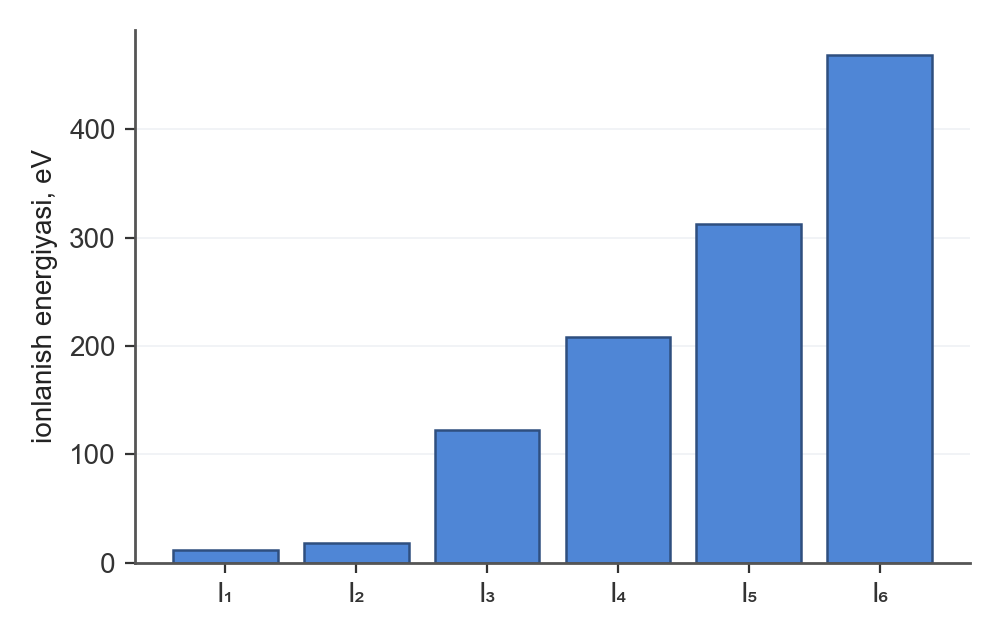
\includegraphics[width=0.86\linewidth]{rasmlar/gen/ie_v11_0.png}\end{center}
A elementining eng yuqori oksidi \textbf{formulasini toping.}

\noindent A)~\textsl{A\textsubscript{2}O} \hfill B)~\textsl{AO} \hfill C)~\textsl{A\textsubscript{2}O\textsubscript{3}} \hfill D)~\textsl{AO\textsubscript{2}}\par
\qsep
\noindent\qn{12.} Massa soni 238 va zaryadi 92 bo`lgan yadro massa soni 206, zaryadi 82 bo`lgan yadroga aylanishida nechta $\alpha$- va $\beta$\textsuperscript{$-$}-zarra chiqaradi?

\noindent A)~\textsl{8$\alpha$ va 6$\beta$} \hfill B)~\textsl{9$\alpha$ va 6$\beta$} \hfill C)~\textsl{8$\alpha$ va 8$\beta$} \hfill D)~\textsl{6$\alpha$ va 8$\beta$}\par
\qsep
\noindent\qn{13.} N\textsubscript{2}O\textsubscript{5} tarkibida azot ning \textbf{valentligini aniqlang.}

\noindent A)~\textsl{\textit{V}} \hfill B)~\textsl{VI} \hfill C)~\textsl{VII} \hfill D)~\textsl{IV}\par
\qsep
\noindent\qn{14.} Nodir gazlar haqida qaysi fikrlar to`g`ri? 1) Geliy eng yengil inert gaz; 2) Argon elektr lampalarida ishlatiladi; 3) Neon atomida 8 ta tashqi elektron bor; 4) Neon reklama naylarida ishlatiladi

\noindent\begin{tabular}{@{}p{0.47\linewidth}@{}p{0.47\linewidth}@{}}
A)~\textsl{1, 3, 4} & B)~\textsl{1, 2, 4} \\
C)~\textsl{1, 2, 3} & D)~\textsl{1, 2, 3, 4} \\
\end{tabular}\par
\qsep
\noindent\qn{15.} Zn(NO\textsubscript{3})\textsubscript{2} qizdirilganda qanday moddalar hosil bo`ladi?

\noindent\begin{tabular}{@{}p{0.47\linewidth}@{}p{0.47\linewidth}@{}}
A)~\textsl{NaNO\textsubscript{2} va O\textsubscript{2}} & B)~\textsl{ZnO, NO\textsubscript{2} va O\textsubscript{2}} \\
C)~\textsl{CuO, NO\textsubscript{2} va O\textsubscript{2}} & D)~\textsl{Ag, NO\textsubscript{2} va O\textsubscript{2}} \\
\end{tabular}\par
\qsep
\noindent\qn{16.} 2ZnS + 3O\textsubscript{2} $\to$ 2ZnO + 2SO\textsubscript{2} reaksiyasida tarkibida 75\% aralashma bo`lgan 77,6 g namuna (asosiy modda ZnS) ishtirok etdi. SO\textsubscript{2} \textbf{massasini (g) toping.}

\noindent A)~\textsl{25,6} \hfill B)~\textsl{6,4} \hfill C)~\textsl{19,2} \hfill D)~\textsl{12,8}\par
\qsep
\noindent\qn{17.} 42,5 g AgNO\textsubscript{3} to`liq parchalanguncha qizdirildi. Qattiq qoldiq \textbf{massasini (g) aniqlang.}

\noindent A)~\textsl{42,5} \hfill B)~\textsl{27} \hfill C)~\textsl{54} \hfill D)~\textsl{13,5}\par
\qsep
\noindent\qn{18.} 2CO + O\textsubscript{2} $\to$ 2CO\textsubscript{2} reaksiyasida 32 g O\textsubscript{2} ishtirok etdi (unum 80\%). CO\textsubscript{2} \textbf{hajmini (l, n.sh.) toping.}

\noindent A)~\textsl{11,2} \hfill B)~\textsl{35,84} \hfill C)~\textsl{71,68} \hfill D)~\textsl{17,92}\par
\qsep
\noindent\qn{19.} NaCl + AgNO\textsubscript{3} $\to$ AgCl + NaNO\textsubscript{3} jarayoni uchun 85 g AgNO\textsubscript{3} olingan. NaCl \textbf{massasini (g) aniqlang.}

\noindent A)~\textsl{58,5} \hfill B)~\textsl{14,62} \hfill C)~\textsl{43,88} \hfill D)~\textsl{29,25}\par
\qsep
\noindent\qn{20.} Reaksiya tenglamasi: C\textsubscript{3}H\textsubscript{8} + 5O\textsubscript{2} $\to$ 3CO\textsubscript{2} + 4H\textsubscript{2}O. Reaksiyaga 11,2 l (n.sh.) C\textsubscript{3}H\textsubscript{8} kirishdi. O\textsubscript{2} \textbf{hajmini (l, n.sh.) hisoblang.}

\noindent A)~\textsl{2,24} \hfill B)~\textsl{56} \hfill C)~\textsl{112} \hfill D)~\textsl{28}\par
\qsep
\noindent\qn{21.} C\textsubscript{2}H\textsubscript{5}OH $\to$ C\textsubscript{2}H\textsubscript{4} + H\textsubscript{2}O jarayoni uchun 46 g C\textsubscript{2}H\textsubscript{5}OH olingan. C\textsubscript{2}H\textsubscript{4} \textbf{hajmini (l, n.sh.) aniqlang.}

\noindent A)~\textsl{44,8} \hfill B)~\textsl{11,2} \hfill C)~\textsl{33,6} \hfill D)~\textsl{22,4}\par
\qsep
\noindent\qn{22.} 32 g CaC\textsubscript{2} suv bilan reaksiyaga kirishganda ajraladigan asetilen \textbf{hajmini (l, n.sh.) aniqlang} (unum 80\%).

\noindent A)~\textsl{8,96} \hfill B)~\textsl{11,2} \hfill C)~\textsl{25,6} \hfill D)~\textsl{22,4}\par
\qsep
\noindent\qn{23.} Rasmda ko`rsatilgan molekulalar o`zaro ta'sirlashganda (H\textsubscript{2}SO\textsubscript{4} ishtirokida) hosil bo`lgan murakkab efir molekulasidagi uglerod atomlarining sp\textsuperscript{3} gibrid orbitallari sonini sp\textsuperscript{2} gibrid orbitallari soniga \textbf{nisbatini aniqlang.}
\begin{center}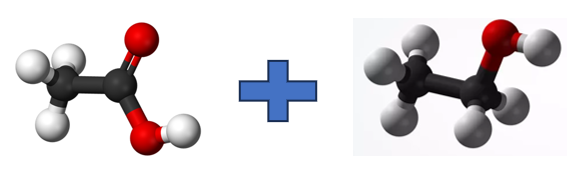
\includegraphics[width=0.86\linewidth]{rasmlar/m_efir.png}\end{center}

\noindent A)~\textsl{3} \hfill B)~\textsl{5} \hfill C)~\textsl{4} \hfill D)~\textsl{2,5}\par
\qsep
\noindent\qn{24.} Aldegid va ketonlar haqida qaysi fikrlar to`g`ri? 1) Aldegidlar qaytarilganda ikkilamchi spirt hosil bo`ladi; 2) Sirka aldegid Kucherov reaksiyasi bilan olinadi; 3) Formaldegid gaz holatda, suvda yaxshi eriydi; 4) Aldegidlar "kumush ko`zgu" reaksiyasini beradi

\noindent A)~\textsl{2, 3, 4} \hfill B)~\textsl{2, 3} \hfill C)~\textsl{1, 2, 3} \hfill D)~\textsl{1, 3}\par
\qsep
\noindent\qn{25.} Karbon kislotalar haqida qaysi fikrlar to`g`ri? 1) Karboksil guruh karbonil va gidroksil guruhlardan iborat; 2) Qattiq suvda sovun yaxshi ko`piklanadi; 3) Olein kislota Br\textsubscript{2} ni biriktiradi; 4) Sirka angidrid ikki molekula sirka kislotadan suv chiqib hosil bo`ladi

\noindent A)~\textsl{1, 2, 3} \hfill B)~\textsl{1, 3, 4} \hfill C)~\textsl{1, 3} \hfill D)~\textsl{2, 4}\par
\qsep
\noindent\qn{26.} 161,2 g tripalmitin natriy ishqori bilan to`liq gidrolizlanganda necha gramm sovun hosil bo`ladi?

\noindent A)~\textsl{55,6} \hfill B)~\textsl{111,2} \hfill C)~\textsl{161,2} \hfill D)~\textsl{166,8}\par
\qsep
\noindent\qn{27.} Quyidagi birikmalardan qaysi biri keton sinfiga kiradi?

\noindent A)~\textsl{C\textsubscript{6}H\textsubscript{5}OH} \hfill B)~\textsl{CH\textsubscript{3}OCH\textsubscript{3}} \hfill C)~\textsl{CH\textsubscript{3}COOH} \hfill D)~\textsl{CH\textsubscript{3}COCH\textsubscript{3}}\par
\qsep
\noindent\qn{28.} Aminlar, aminokislotalar va oqsillar haqida qaysi fikrlar to`g`ri? 1) Glitsin optik faol; 2) Dipeptidda 2 ta peptid bog` bor; 3) Anilin bromli suv bilan oq cho`kma beradi; 4) Aminokislotalar faqat kislotali xossaga ega

\noindent A)~\textsl{2, 4} \hfill B)~\textsl{3, 4} \hfill C)~\textsl{3} \hfill D)~\textsl{1, 2}\par
\qsep
\noindent\qn{29.} 26 g C\textsubscript{2}H\textsubscript{2} dan quyidagi ikki bosqichda C\textsubscript{2}H\textsubscript{6} olinadi: 1) C\textsubscript{2}H\textsubscript{2} + H\textsubscript{2} $\to$ C\textsubscript{2}H\textsubscript{4} (unum 50\%); 2) C\textsubscript{2}H\textsubscript{4} + H\textsubscript{2} $\to$ C\textsubscript{2}H\textsubscript{6} (unum 50\%). Oxirgi mahsulot C\textsubscript{2}H\textsubscript{6} ning \textbf{hajmini (l, n.sh.) toping.}

\noindent A)~\textsl{11,2} \hfill B)~\textsl{5,6} \hfill C)~\textsl{22,4} \hfill D)~\textsl{2,8}\par
\qsep
\noindent\qn{30.} Laboratoriyada vodorod olish uchun qaysi moddalar ishlatiladi?
\noindent A)~\textsl{CaCO\textsubscript{3} + HCl}\par
\noindent B)~\textsl{CH\textsubscript{3}COONa + NaOH (qizdirish)}\par
\noindent C)~\textsl{KMnO\textsubscript{4} (qizdirish)}\par
\noindent D)~\textsl{Zn + HCl}\par
\qsep
\noindent\qn{31.} Rasmdagi usul bilan qaysi moddani eritmadan ajratib olish mumkin?
\begin{center}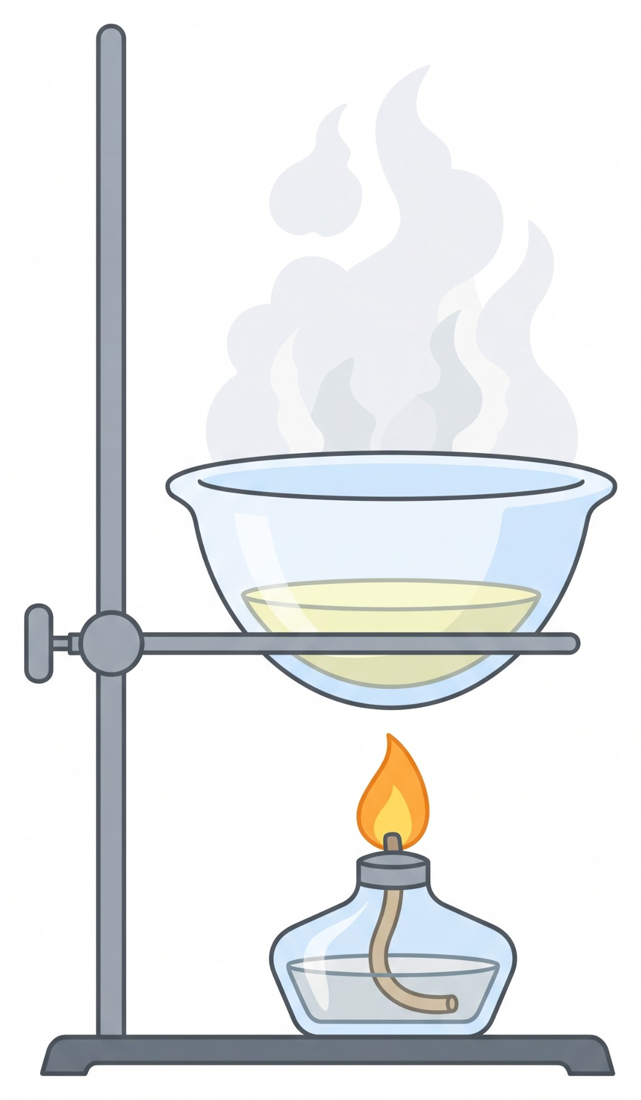
\includegraphics[width=0.86\linewidth]{rasmlar/darslik/d_bugla.png}\end{center}
\noindent A)~\textsl{osh tuzini tuz eritmasidan}\par
\noindent B)~\textsl{kerosinni suvdan}\par
\noindent C)~\textsl{qumni suvdan}\par
\noindent D)~\textsl{suvni osh tuzi eritmasidan (toza holda)}\par
\qsep
\noindent\qn{32.} NaNO\textsubscript{3} ning 50\% li eritmasidan 200 g 10\% li eritma tayyorlash uchun necha gramm suv kerak?

\noindent A)~\textsl{40} \hfill B)~\textsl{200} \hfill C)~\textsl{160} \hfill D)~\textsl{320   ---}\par
\qsep
\end{multicols}
\medskip
\noindent\setlength{\fboxsep}{0pt}\fbox{\begin{tabular}{p{0.74\linewidth}|p{0.2\linewidth}}
\parbox[t]{0.72\linewidth}{\vspace{3pt}\textbf{Topshiriqlar (33--35) va javob variant (A--F)larini o`zaro to`g`ri moslashtiring.} K\textsubscript{2}CO\textsubscript{3} va BaCO\textsubscript{3} dan iborat 60,1 g aralashma mo`l xlorid kislota bilan to`liq reaksiyaga kirishdi.
\vspace{3pt}} & \parbox[t]{0.19\linewidth}{\vspace{3pt}A~\textsl{7,84}\\[3pt]
B~\textsl{52,77}\\[3pt]
C~\textsl{255,5}\\[3pt]
D~\textsl{11,76}\\[3pt]
E~\textsl{6,27}\\[3pt]
F~\textsl{204,4}}\\ \hline
\parbox[t]{0.72\linewidth}{\vspace{2pt}\textbf{33. Ajralgan gaz hajmini (l, n.sh.) aniqlang.}\vspace{2pt}} & \\ \hline
\parbox[t]{0.72\linewidth}{\vspace{2pt}\textbf{34. Aralashmani to`liq eritish uchun sarflangan 10\% li HCl eritmasining massasini (g) aniqlang (M(HCl) = 36,5 g/mol).}\vspace{2pt}} & \\ \hline
\parbox[t]{0.72\linewidth}{\vspace{2pt}\textbf{35. Reaksiyadan so`ng eritmadagi tuzlar umumiy massasini (g) aniqlang.}\vspace{2pt}} & 
\end{tabular}}
\par\bigskip
\noindent\qn{36.} K\textsubscript{2}Cr\textsubscript{2}O\textsubscript{7} + FeSO\textsubscript{4} + H\textsubscript{2}SO\textsubscript{4} $\to$ Cr\textsubscript{2}(SO\textsubscript{4})\textsubscript{3} + Fe\textsubscript{2}(SO\textsubscript{4})\textsubscript{3} + K\textsubscript{2}SO\textsubscript{4} + H\textsubscript{2}O reaksiya tenglamasini tenglang va barcha koeffitsiyentlar \textbf{yig`indisini aniqlang.}
\javob\qsep
\noindent\qn{37.} 5,4 g Al reaksiyaga kirishdi (2Al + 6HCl $\to$ 2AlCl\textsubscript{3} + 3H\textsubscript{2}). Ajralgan H\textsubscript{2} \textbf{hajmini (l, n.sh.) hisoblang} (unum 80\%).
\javob\qsep
\noindent\qn{38.} Al, Fe va Cu dan iborat aralashma mo`l NaOH eritmasi bilan ta'sirlashganda 6,72 l (n.sh.) vodorod ajraldi; xuddi shunday massadagi aralashma mo`l HCl bilan ta'sirlashganda 11,2 l (n.sh.) vodorod ajraldi, erimay qolgan qoldiq (mis) massasi 6,4 g. Aralashmaning dastlabki \textbf{massasini (g) toping.}
\javob\qsep
\noindent\qn{39.} 180 g glyukoza spirtli bijg`ish natijasida etanolga (unum 80\%), hosil bo`lgan etanol esa sirka kislotagacha (unum 75\%) aylantirildi. Olingan kislotani to`liq neytrallash uchun NaOH ning \textbf{massasini (g) toping.}
\javob\qsep
\noindent\qn{40.} Polivinilxlorid polimerining (polimerlanish darajasi 1000) 62,5 g namunasini olish uchun polimerlanish unumi 50\% bo`lganda qancha monomer (C\textsubscript{2}H\textsubscript{3}Cl) kerak (g)?
\javob\qsep
\par\bigskip\begin{center}\textbf{\fontsize{13}{15}\selectfont YOZMA ISH}\end{center}
\noindent\qn{41.} \textbf{Topshiriqni bajarish jarayonida barcha reaksiya tenglamalarini yozing. Miqdoriy va arifmetik hisoblashlarni (unga asos bo`lgan usul yoki formulani ko`rsatgan holda) uzviy ketma-ketlikda bajaring.}\par\smallskip
2 l hajmli idishda N\textsubscript{2} + 3H\textsubscript{2} $\rightleftarrows$ 2NH\textsubscript{3} reaksiyasi muvozanat holatiga keldi. Muvozanatda idishda 4 mol N\textsubscript{2}, 4 mol H\textsubscript{2} va 8 mol NH\textsubscript{3} bor.\par
\noindent 1)\ Muvozanat konstantasini (K) hisoblang.\par
\noindent 2)\ Azot va vodorodning boshlang`ich konsentratsiyalarini (mol/l) aniqlang. H\textsubscript{2} ning boshlang`ich massasini (g) ham toping.\par
\noindent 3)\ Vodorodning necha foizi reaksiyaga kirishgan?\par
\noindent 4)\ Hosil bo`lgan ammiakning hammasi 800 g suvda eritildi. Eritmadagi ammiakning massa ulushini (\%) hisoblang. Ajralgan NH\textsubscript{3} hajmini (l, n.sh.) ham toping.\par
\noindent 5)\ Shu eritmani (NH\textsubscript{4})\textsubscript{2}SO\textsubscript{4} hosil bo`lguncha neytrallash uchun 20\% li H\textsubscript{2}SO\textsubscript{4} eritmasidan necha gramm kerak? Idish hajmi 2 marta kamaytirilsa, to`g`ri reaksiya tezligi (elementar deb hisoblang) necha marta ortadi?\par
\diqqat{Mazkur topshiriq kengaytirilgan javobni talab etib, uning yechilish usuli va shu usul asosidagi barcha hisoblash amallari javoblar varaqasida aks etishi lozim.}\qsep
\noindent\qn{42.} Quyidagi o`zgarishlar zanjirida \textit{X}, \textit{Y}, \textit{Z} noma'lum organik moddalar:\par
\[\setlength{\fboxsep}{0pt}\text{CaC\textsubscript{2}}\xrightarrow{\text{H\textsubscript{2}O}}\text{\textit{X}}\xrightarrow{\text{H\textsubscript{2}O, Hg\textsuperscript{2+}}}\text{\textit{Y}}\xrightarrow{\text{Ag\textsubscript{2}O, NH\textsubscript{3}}}\text{\textit{Z}}\xrightarrow{\text{Cl\textsubscript{2}, P}}\text{ClCH\textsubscript{2}COOH}\]
\noindent 1)\ CaC\textsubscript{2} $\to$ \textit{X} : reaksiya tenglamasini yozing; hosil bo`lgan moddani nomlang.\par
\noindent 2)\ \textit{X} $\to$ \textit{Y} : reaksiya tenglamasini yozing; hosil bo`lgan moddani nomlang.\par
\noindent 3)\ \textit{Y} $\to$ \textit{Z} : reaksiya tenglamasini yozing; hosil bo`lgan moddani nomlang.\par
\noindent 4)\ \textit{Z} $\to$ ClCH\textsubscript{2}COOH : reaksiya tenglamasini yozing; hosil bo`lgan moddani nomlang.\par
\diqqat{Mazkur topshiriq kengaytirilgan javobni talab etib, uning yechilish usuli va shu usul asosidagi barcha hisoblash amallari javoblar varaqasida aks etishi lozim.}\qsep
\noindent\qn{43.} \textbf{Topshiriqni bajarish jarayonida barcha reaksiya tenglamalarini yozing. Miqdoriy va arifmetik hisoblashlarni (unga asos bo`lgan usul yoki formulani ko`rsatgan holda) uzviy ketma-ketlikda bajaring.}\par\smallskip
Uch probirkada (\textit{X}, \textit{Y}, \textit{Z}) natriy yoki kaliy tuzlarining eritmalari bor: Na\textsubscript{2}CO\textsubscript{3}, Na\textsubscript{3}PO\textsubscript{4}, NaBr (tartibsiz). Har bir eritmaga reagentlar ta'sir ettirildi, kuzatuvlar jadvalda:\par
\begin{center}
\renewcommand{\arraystretch}{1.15}
\begin{tabular}{|c|c|c|c|}\hline
\textbf{Reagent} & \textbf{\textit{X}} & \textbf{\textit{Y}} & \textbf{\textit{Z}} \\ \hline
AgNO\textsubscript{3} & och sariq cho`kma (AgBr) & oq-sarg`ish cho`kma & sariq cho`kma (Ag\textsubscript{3}PO\textsubscript{4}) \\ \hline
BaCl\textsubscript{2} & --- & oq cho`kma (BaCO\textsubscript{3}) & oq cho`kma \\ \hline
HCl & --- & gaz (CO\textsubscript{2}) ajraladi & --- \\ \hline
\end{tabular}
\end{center}
\noindent 1)\ \textit{X}, \textit{Y}, \textit{Z} probirkalardagi moddalarni aniqlang va kuzatilgan reaksiyalarning ionli tenglamalarini yozing.\par
\noindent 2)\ \textit{X} probirkadagi tuz 0,2 mol miqdorda olingan. Unga mo`l AgNO\textsubscript{3} qo`shilganda hosil bo`lgan cho`kma massasini (g) toping.\par
\noindent 3)\ Uchala eritmaning har biriga 0,2 mol dan solingan bo`lsa, mo`l AgNO\textsubscript{3} qo`shilganda hosil bo`ladigan barcha cho`kmalarning umumiy massasini (g) toping (ularning formulalarini yozing).\par
\noindent 4)\ Eritmalarda kuzatilgan hodisalarni (cho`kma yoki gaz hosil bo`lishi) tushuntiring: qaysi ion qaysi reagent bilan qanday birikma hosil qiladi? Shu usul bilan ionlarni aniqlash qoidasini yozing.\par
\noindent 5)\ Uchala eritmaning har biriga 0,2 mol dan solingan. AgNO\textsubscript{3} bilan cho`kadigan ionlarni to`liq cho`ktirish uchun 10\% li AgNO\textsubscript{3} eritmasidan necha gramm kerak?\par
\diqqat{Mazkur topshiriq kengaytirilgan javobni talab etib, uning yechilish usuli va shu usul asosidagi barcha hisoblash amallari javoblar varaqasida aks etishi lozim.}\qsep
\newpage
\renewcommand{\curvar}{12-variant}
\thispagestyle{first}
\noindent\textit{Davriy jadvaldan foydalanish mumkin.}
\par\smallskip
\begin{multicols}{2}
\noindent\qn{1.} Qaysi juftliklarda reaksiya boradi? 1) Pb va ZnCl\textsubscript{2}; 2) Al va CuSO\textsubscript{4}; 3) Zn va CuSO\textsubscript{4}; 4) Ag va CuSO\textsubscript{4}

\noindent A)~\textsl{1, 2} \hfill B)~\textsl{4} \hfill C)~\textsl{1, 2, 4} \hfill D)~\textsl{2, 3}\par
\qsep
\noindent\qn{2.} Jadvalda bog`lar hosil qiluvchi atomlarning elektrmanfiyliklari berilgan:
\begin{center}
\renewcommand{\arraystretch}{1.15}
\fitbox{\begin{tabular}{|c|c|c|}\hline
\textbf{Bog`} & \textbf{EM (1-atom)} & \textbf{EM (2-atom)} \\ \hline
H--Cl & 2,1 & 3 \\ \hline
H--O & 2,1 & 3,5 \\ \hline
H--F & 2,1 & 4 \\ \hline
C--O & 2,5 & 3,5 \\ \hline
\end{tabular}}
\end{center}
Qaysi bog` eng qutbli (eng ko`p ionli xarakterga ega)?

\noindent A)~\textsl{H--Cl} \hfill B)~\textsl{H--O} \hfill C)~\textsl{C--O} \hfill D)~\textsl{H--F}\par
\qsep
\noindent\qn{3.} Rasmda neytral atom elektron qavatlarining orbital diagrammasi (kataklar -- orbitallar, o`qlar -- elektronlar) berilgan.
\begin{center}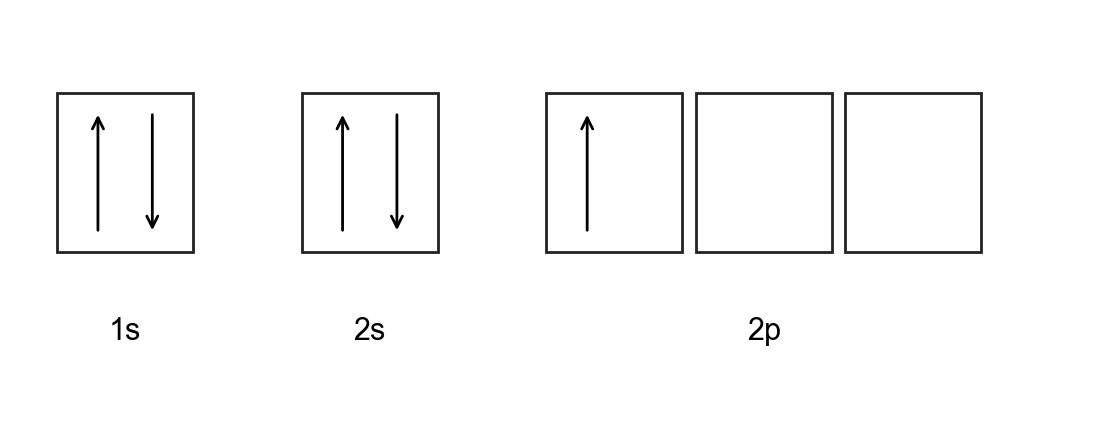
\includegraphics[width=0.86\linewidth]{rasmlar/gen/or_588848.png}\end{center}
Diagramma qaysi element atomiga tegishli?

\noindent A)~\textsl{kislorod} \hfill B)~\textsl{bor} \hfill C)~\textsl{azot} \hfill D)~\textsl{uglerod}\par
\qsep
\noindent\qn{4.} Gazlar aralashmasi tarkibi jadvalda berilgan (n.sh.):
\begin{center}
\renewcommand{\arraystretch}{1.15}
\fitbox{\begin{tabular}{|c|c|}\hline
\textbf{Gaz} & \textbf{Hajmi, l} \\ \hline
N\textsubscript{2} & 1 \\ \hline
H\textsubscript{2} & 1 \\ \hline
SO\textsubscript{2} & 3 \\ \hline
\end{tabular}}
\end{center}
Aralashmaning havoga nisbatan \textbf{zichligini aniqlang} (M(havo) = 29 g/mol).

\noindent A)~\textsl{3,06} \hfill B)~\textsl{0,77} \hfill C)~\textsl{1,53} \hfill D)~\textsl{44,4}\par
\qsep
\noindent\qn{5.} FeSO\textsubscript{4}$\cdot$7H\textsubscript{2}O kristallogidratida kristallizatsion suvning massa \textbf{ulushini (\%) aniqlang.}

\noindent A)~\textsl{54,7} \hfill B)~\textsl{22,7} \hfill C)~\textsl{82,9} \hfill D)~\textsl{45,3}\par
\qsep
\noindent\qn{6.} Konsentratsiyasi bir xil (0,1 mol/l) eritmalarning pH qiymatlari diagrammada berilgan.
\begin{center}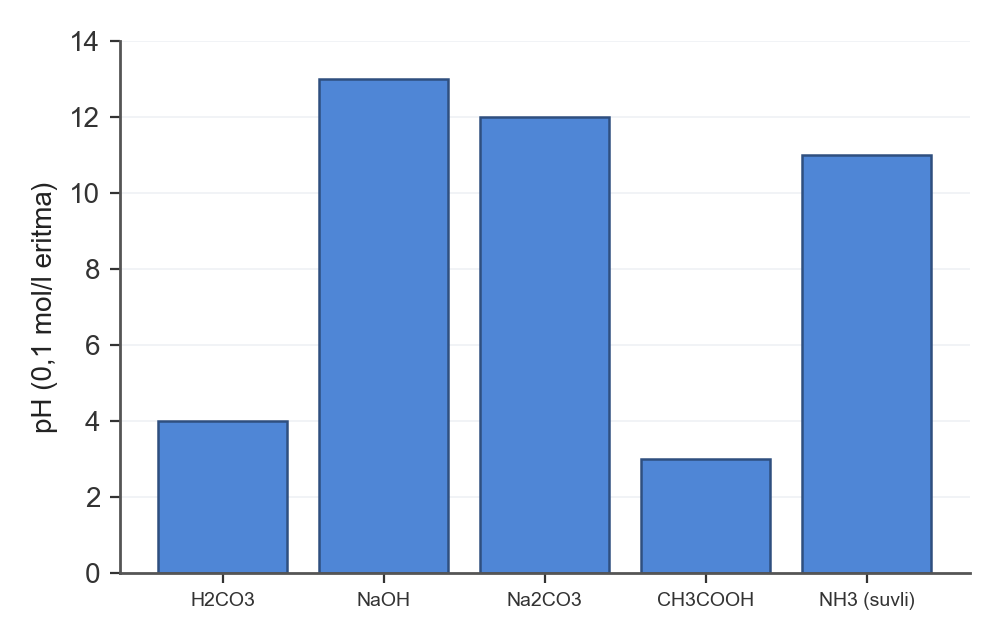
\includegraphics[width=0.86\linewidth]{rasmlar/gen/pb_v12_0.png}\end{center}
Qaysi eritmada [H\textsuperscript{+}] eng katta?

\noindent\begin{tabular}{@{}p{0.47\linewidth}@{}p{0.47\linewidth}@{}}
A)~\textsl{CH\textsubscript{3}COOH} & B)~\textsl{NH\textsubscript{3} (suvli)} \\
C)~\textsl{Na\textsubscript{2}CO\textsubscript{3}} & D)~\textsl{H\textsubscript{2}CO\textsubscript{3}} \\
\end{tabular}\par
\qsep
\noindent\qn{7.} Fosfor (\textit{Z} = 15) atomida nechta juftlashmagan elektron bor?

\noindent A)~\textsl{4} \hfill B)~\textsl{2} \hfill C)~\textsl{5} \hfill D)~\textsl{3}\par
\qsep
\noindent\qn{8.} 4 g NaOH ni to`liq neytrallash uchun 6 g CH\textsubscript{3}COOH sarflandi. CH\textsubscript{3}COOH ning ekvivalent \textbf{massasini (g/mol) aniqlang.}

\noindent A)~\textsl{60} \hfill B)~\textsl{120} \hfill C)~\textsl{30} \hfill D)~\textsl{6}\par
\qsep
\noindent\qn{9.} 100 g 10\% li MgSO\textsubscript{4} eritmasiga 50 g shu tuzning o`zi qo`shilib eritildi. Hosil bo`lgan eritmaning massa \textbf{ulushini (\%) aniqlang.}

\noindent A)~\textsl{40} \hfill B)~\textsl{60} \hfill C)~\textsl{30} \hfill D)~\textsl{32}\par
\qsep
\noindent\qn{10.} 1,5 mol H\textsubscript{2}O tarkibida necha mol atom bor?

\noindent A)~\textsl{3} \hfill B)~\textsl{4,5} \hfill C)~\textsl{6} \hfill D)~\textsl{1,5}\par
\qsep
\noindent\qn{11.} Fe plastinka 8 g CuSO\textsubscript{4} ni tutgan eritmaga tushirildi va Cu to`liq ajralib chiqquncha ushlab turildi. Plastinka massasi necha gramm ortadi?

\noindent A)~\textsl{0,4} \hfill B)~\textsl{0,8} \hfill C)~\textsl{0,2} \hfill D)~\textsl{8}\par
\qsep
\noindent\qn{12.} H\textsubscript{3}PO\textsubscript{3} tarkibida P ning oksidlanish \textbf{darajasini aniqlang.}

\noindent A)~\textsl{+3} \hfill B)~\textsl{$-$1} \hfill C)~\textsl{+3 va +5} \hfill D)~\textsl{+4}\par
\qsep
\noindent\qn{13.} Mishyak (\textit{Z} = 33) atomi elektron konfiguratsiyasida jami nechta juftlashgan elektron bor?

\noindent A)~\textsl{31} \hfill B)~\textsl{29} \hfill C)~\textsl{30} \hfill D)~\textsl{32}\par
\qsep
\noindent\qn{14.} Qaysi juftliklar o`zaro reaksiyaga kirishadi? 1) Fe va HCl; 2) Fe\textsubscript{2}O\textsubscript{3} va H\textsubscript{2}O; 3) CuSO\textsubscript{4} va NaOH; 4) CuO va H\textsubscript{2}

\noindent A)~\textsl{1, 2, 4} \hfill B)~\textsl{2, 3} \hfill C)~\textsl{1, 3, 4} \hfill D)~\textsl{1, 3}\par
\qsep
\noindent\qn{15.} Cu(NO\textsubscript{3})\textsubscript{2} qizdirilganda qanday moddalar hosil bo`ladi?

\noindent\begin{tabular}{@{}p{0.47\linewidth}@{}p{0.47\linewidth}@{}}
A)~\textsl{CuO, NO\textsubscript{2} va O\textsubscript{2}} & B)~\textsl{ZnO, NO\textsubscript{2} va O\textsubscript{2}} \\
C)~\textsl{Ag, NO\textsubscript{2} va O\textsubscript{2}} & D)~\textsl{NaNO\textsubscript{2} va O\textsubscript{2}} \\
\end{tabular}\par
\qsep
\noindent\qn{16.} 6,2 g fosfor yondirilib, hosil bo`lgan oksid suvda eritildi (ortofosfat kislota), so`ng 0,3 mol NaOH qo`shildi. Hosil bo`lgan NaH\textsubscript{2}PO\textsubscript{4} \textbf{massasini (g) aniqlang.}

\noindent A)~\textsl{24} \hfill B)~\textsl{6} \hfill C)~\textsl{12} \hfill D)~\textsl{32,8}\par
\qsep
\noindent\qn{17.} 2NaBr + Cl\textsubscript{2} $\to$ 2NaCl + Br\textsubscript{2} jarayoni uchun 22,4 l (n.sh.) Cl\textsubscript{2} olingan (unum 75\%). Br\textsubscript{2} \textbf{massasini (g) aniqlang.}

\noindent A)~\textsl{160} \hfill B)~\textsl{120} \hfill C)~\textsl{240} \hfill D)~\textsl{60}\par
\qsep
\noindent\qn{18.} Li va Na dan iborat 6,7 g aralashma suv bilan reaksiyaga kirishdi. Ajralgan vodorodning \textbf{hajmini (l, n.sh.) aniqlang.}

\noindent A)~\textsl{11,2} \hfill B)~\textsl{2,8} \hfill C)~\textsl{5,6} \hfill D)~\textsl{3,35}\par
\qsep
\noindent\qn{19.} Alyuminiy va rux dan iborat 18,4 g aralashma mo`l xlorid kislotada eritilganda 11,2 l (n.sh.) vodorod ajraldi. Aralashmadagi alyuminiyning massa \textbf{ulushini (\%) aniqlang.}

\noindent A)~\textsl{70,7} \hfill B)~\textsl{29,3} \hfill C)~\textsl{14,7} \hfill D)~\textsl{5,4}\par
\qsep
\noindent\qn{20.} Uglevodorodning 4,4 g massasi yondirilganda 13,2 g CO\textsubscript{2} va 7,2 g H\textsubscript{2}O hosil bo`ldi. Uglevodorod molekulasidagi uglerod atomlari \textbf{sonini toping} (M = 44 g/mol).

\noindent A)~\textsl{4} \hfill B)~\textsl{3} \hfill C)~\textsl{2} \hfill D)~\textsl{8}\par
\qsep
\noindent\qn{21.} CH\textsubscript{3}--CH\textsubscript{2}--CH(CH\textsubscript{3})--CHO birikmaning sistematik nomi qaysi qatorda to`g`ri keltirilgan?

\noindent\begin{tabular}{@{}p{0.47\linewidth}@{}p{0.47\linewidth}@{}}
A)~\textsl{3-metilbutanal} & B)~\textsl{2-metilbutanal} \\
C)~\textsl{pentanal} & D)~\textsl{2-metilbutanon} \\
\end{tabular}\par
\qsep
\noindent\qn{22.} 6,5 g C\textsubscript{2}H\textsubscript{2} dan quyidagi ikki bosqichda C\textsubscript{2}H\textsubscript{5}OH olinadi: 1) C\textsubscript{2}H\textsubscript{2} + H\textsubscript{2}O $\to$ CH\textsubscript{3}CHO (unum 80\%); 2) CH\textsubscript{3}CHO + H\textsubscript{2} $\to$ C\textsubscript{2}H\textsubscript{5}OH (unum 50\%). Oxirgi mahsulot C\textsubscript{2}H\textsubscript{5}OH ning \textbf{massasini (g) toping.}

\noindent A)~\textsl{5,75} \hfill B)~\textsl{9,2} \hfill C)~\textsl{11,5} \hfill D)~\textsl{4,6}\par
\qsep
\noindent\qn{23.} CH\textsubscript{3}COONa + NaOH (t) reaksiyasi natijasida qaysi organik modda hosil bo`ladi?

\noindent\begin{tabular}{@{}p{0.47\linewidth}@{}p{0.47\linewidth}@{}}
A)~\textsl{sirka aldegid} & B)~\textsl{metan} \\
C)~\textsl{etilen} & D)~\textsl{benzoy kislota} \\
\end{tabular}\par
\qsep
\noindent\qn{24.} Aldegid va ketonlar haqida qaysi fikrlar to`g`ri? 1) Aseton Cu(OH)\textsubscript{2} ni qaytaradi; 2) Aldegidlar "kumush ko`zgu" reaksiyasini beradi; 3) Ketonlar kuchsiz oksidlovchilar bilan oksidlanmaydi; 4) Formalin --- formaldegidning 40\% li eritmasi

\noindent A)~\textsl{1, 2, 3} \hfill B)~\textsl{2, 3, 4} \hfill C)~\textsl{1, 3, 4} \hfill D)~\textsl{2, 4}\par
\qsep
\noindent\qn{25.} Reaksiya tenglamasi: C\textsubscript{2}H\textsubscript{5}COOH + KOH $\to$ C\textsubscript{2}H\textsubscript{5}COOK + H\textsubscript{2}O. Reaksiyaga 56 g KOH kirishdi. C\textsubscript{2}H\textsubscript{5}COOH \textbf{miqdorini (mol) hisoblang.}

\noindent A)~\textsl{2} \hfill B)~\textsl{0,5} \hfill C)~\textsl{1,5} \hfill D)~\textsl{1}\par
\qsep
\noindent\qn{26.} Murakkab efirlar va yog`lar haqida qaysi fikrlar to`g`ri? 1) Suyuq yog`lar to`yinmagan kislotalardan hosil bo`lgan; 2) Etilatsetat efir hidli suyuqlik; 3) Murakkab efirlarning gidrolizi ishqoriy muhitda qaytmas; 4) Dietil efir spirtdan yuqori haroratda qaynaydi

\noindent A)~\textsl{2, 3, 4} \hfill B)~\textsl{1, 4} \hfill C)~\textsl{1, 2, 3} \hfill D)~\textsl{1, 3, 4}\par
\qsep
\noindent\qn{27.} Quyidagi birikmalardan qaysi biri aldegid sinfiga kiradi?

\noindent\begin{tabular}{@{}p{0.47\linewidth}@{}p{0.47\linewidth}@{}}
A)~\textsl{CH\textsubscript{3}CHO} & B)~\textsl{CH\textsubscript{3}COCH\textsubscript{3}} \\
C)~\textsl{C\textsubscript{6}H\textsubscript{5}OH} & D)~\textsl{H\textsubscript{2}NCH\textsubscript{2}COOH} \\
\end{tabular}\par
\qsep
\noindent\qn{28.} Quyidagi birikmalardan qaysi biri murakkab efir sinfiga kiradi?

\noindent\begin{tabular}{@{}p{0.47\linewidth}@{}p{0.47\linewidth}@{}}
A)~\textsl{C\textsubscript{6}H\textsubscript{5}OH} & B)~\textsl{CH\textsubscript{3}COOH} \\
C)~\textsl{CH\textsubscript{3}COOC\textsubscript{2}H\textsubscript{5}} & D)~\textsl{CH\textsubscript{3}CHO} \\
\end{tabular}\par
\qsep
\noindent\qn{29.} Yuqori molekulyar birikmalar haqida qaysi fikrlar to`g`ri? 1) Kapron poliamid tola; 2) Teflon --- polivinilxlorid; 3) Fenolformaldegid smola polikondensatsiya mahsuloti; 4) Polimerning M = zveno M $\cdot$ polimerlanish darajasi

\noindent A)~\textsl{1, 3} \hfill B)~\textsl{3, 4} \hfill C)~\textsl{2, 3, 4} \hfill D)~\textsl{1, 3, 4}\par
\qsep
\noindent\qn{30.} Uch probirkada (\textit{X}, \textit{Y}, \textit{Z}) NaCl, NaBr, NaI eritmalari bor (tartibsiz). Ularga AgNO\textsubscript{3} ta'sir ettirildi. Kuzatuvlar jadvalda:
\begin{center}
\renewcommand{\arraystretch}{1.15}
\fitbox{\begin{tabular}{|c|c|}\hline
\textbf{Probirka} & \textbf{AgNO\textsubscript{3} qo`shilganda} \\ \hline
\textit{X} & och sariq cho`kma \\ \hline
\textit{Y} & oq cho`kma \\ \hline
\textit{Z} & sariq cho`kma \\ \hline
\end{tabular}}
\end{center}
\textit{X}, \textit{Y}, \textit{Z} probirkalardagi \textbf{moddalarni aniqlang.}
\noindent A)~\textsl{\textit{X} -- NaBr, \textit{Y} -- NaCl, \textit{Z} -- NaI}\par
\noindent B)~\textsl{\textit{X} -- NaI, \textit{Y} -- NaCl, \textit{Z} -- NaBr}\par
\noindent C)~\textsl{\textit{X} -- NaBr, \textit{Y} -- NaI, \textit{Z} -- NaCl}\par
\noindent D)~\textsl{\textit{X} -- NaCl, \textit{Y} -- NaBr, \textit{Z} -- NaI}\par
\qsep
\noindent\qn{31.} Kimyo laboratoriyasida ishlash qoidalari haqida qaysi fikrlar to`g`ri? 1) Kuygan joy ko`p suv bilan yuviladi; 2) Ishqor teriga tushsa, qo`l suv bilan yuviladi; 3) Zaharli gaz ajraladigan tajriba mo`rili shkafda o`tkaziladi; 4) Konsentrlangan kislotani suvga ohista, aralashtirib quyiladi

\noindent\begin{tabular}{@{}p{0.47\linewidth}@{}p{0.47\linewidth}@{}}
A)~\textsl{1, 2, 3} & B)~\textsl{1, 3, 4} \\
C)~\textsl{2, 3, 4} & D)~\textsl{1, 2, 3, 4} \\
\end{tabular}\par
\qsep
\noindent\qn{32.} Rasmda aralashmani ajratish usuli ko`rsatilgan. Bu \textbf{usulni toping.}
\begin{center}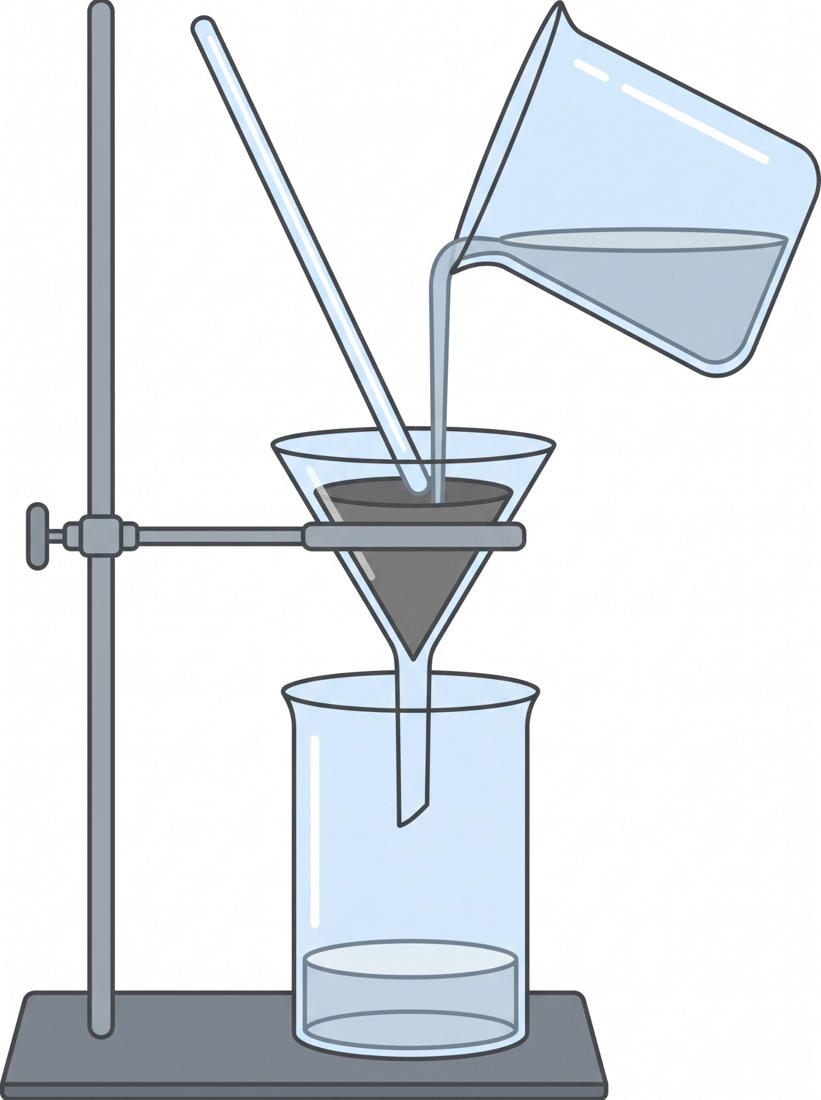
\includegraphics[width=0.86\linewidth]{rasmlar/darslik/d_filtr.png}\end{center}
\noindent A)~\textsl{distillash}\par
\noindent B)~\textsl{magnit yordamida ajratish}\par
\noindent C)~\textsl{filtrlash}\par
\noindent D)~\textsl{bug`latish   ---}\par
\qsep
\end{multicols}
\medskip
\noindent\setlength{\fboxsep}{0pt}\fbox{\begin{tabular}{p{0.74\linewidth}|p{0.2\linewidth}}
\parbox[t]{0.72\linewidth}{\vspace{3pt}\textbf{Topshiriqlar (33--35) va javob variant (A--F)larini o`zaro to`g`ri moslashtiring.} Alyuminiy va temir (Al va Fe) dan iborat 12,45 g qotishma mo`l H\textsubscript{2}SO\textsubscript{4} eritmasida eritilganda 8,4 l (n.sh.) gaz ajraldi.
\vspace{3pt}} & \parbox[t]{0.19\linewidth}{\vspace{3pt}A~\textsl{48,45}\\[3pt]
B~\textsl{183,75}\\[3pt]
C~\textsl{48,8}\\[3pt]
D~\textsl{91,88}\\[3pt]
E~\textsl{32,53}\\[3pt]
F~\textsl{38,76}}\\ \hline
\parbox[t]{0.72\linewidth}{\vspace{2pt}\textbf{33. Qotishmadagi Al massa ulushini (\%) aniqlang.}\vspace{2pt}} & \\ \hline
\parbox[t]{0.72\linewidth}{\vspace{2pt}\textbf{34. Reaksiya uchun sarflangan 20\% li H\textsubscript{2}SO\textsubscript{4} massasini (g) aniqlang.}\vspace{2pt}} & \\ \hline
\parbox[t]{0.72\linewidth}{\vspace{2pt}\textbf{35. Eritmadagi tuzlarning umumiy massasini (g) aniqlang.}\vspace{2pt}} & 
\end{tabular}}
\par\bigskip
\noindent\qn{36.} Fe + H\textsubscript{2}SO\textsubscript{4} $\to$ Fe\textsubscript{2}(SO\textsubscript{4})\textsubscript{3} + SO\textsubscript{2} + H\textsubscript{2}O reaksiya tenglamasini tenglang. Oksidlovchi va qaytaruvchi oldidagi koeffitsiyentlar \textbf{yig`indisini aniqlang.}
\javob\qsep
\noindent\qn{37.} CuSO\textsubscript{4} eritmasi inert elektrodlar yordamida 2 A tok kuchi bilan 9650 s elektroliz qilindi. Katodda ajralgan Cu massasi (g) \textbf{ni toping.}
\javob\qsep
\noindent\qn{38.} CaCO\textsubscript{3} va MgCO\textsubscript{3} dan iborat 18,4 g aralashma doimiy massagacha qizdirilganda qoldiq massasi 9,6 g bo`ldi. Aralashmadagi CaCO\textsubscript{3} ning \textbf{massasini (g) toping.}
\javob\qsep
\noindent\qn{39.} 4,4 g etanal Ag\textsubscript{2}O ning ammiakli eritmasi bilan to`liq oksidlanganda hosil bo`lgan kumush \textbf{massasini (g) aniqlang.}
\javob\qsep
\noindent\qn{40.} 1,5 mol asetilendan Zelinskiy usuli bilan (100\% unum) benzol olindi. Benzol \textbf{massasini (g) aniqlang.}
\javob\qsep
\par\bigskip\begin{center}\textbf{\fontsize{13}{15}\selectfont YOZMA ISH}\end{center}
\noindent\qn{41.} \textbf{Topshiriqni bajarish jarayonida barcha reaksiya tenglamalarini yozing. Miqdoriy va arifmetik hisoblashlarni (unga asos bo`lgan usul yoki formulani ko`rsatgan holda) uzviy ketma-ketlikda bajaring.}\par\smallskip
14,35 g ZnSO\textsubscript{4}$\cdot$7H\textsubscript{2}O 400 g suvda eritildi.\par
\noindent 1)\ Hosil bo`lgan eritmadagi ZnSO\textsubscript{4} ning massa ulushini (\%) toping.\par
\noindent 2)\ Eritmaga mo`l BaCl\textsubscript{2} eritmasi qo`shildi. Hosil bo`lgan cho`kma massasini (g) toping. Eritmadagi kation miqdorini (mol) ham toping.\par
\noindent 3)\ Xuddi shunday eritmaga ekvivalent miqdorda NaOH qo`shilganda hosil bo`lgan Zn(OH)\textsubscript{2} cho`kmasining massasini (g) toping.\par
\noindent 4)\ Eritmaga Mg plastinka tushirildi (ZnSO\textsubscript{4} tuzidagi metall to`liq siqib chiqarildi). Plastinka massasi qanchaga (g) o`zgargan? Dastlabki eritma massasini (g) ham ayting.\par
\noindent 5)\ Kristallogidratdagi kristallizatsion suvning massa ulushini (\%) va unda suv molekulalari sonini toping. Shu miqdor kristallogidrat suvsizlantirilganda massa necha gramm kamayadi?\par
\diqqat{Mazkur topshiriq kengaytirilgan javobni talab etib, uning yechilish usuli va shu usul asosidagi barcha hisoblash amallari javoblar varaqasida aks etishi lozim.}\qsep
\noindent\qn{42.} Reaksiya tenglamalarini tugallang va tenglang. Hosil bo`lgan organik moddalarning tuzilish formulalarini yozing va ularni nomlang.\par
\noindent 1)\ CH\textsubscript{3}COOCH\textsubscript{3} + NaOH $\xrightarrow{\text{t}}$\par
\noindent 2)\ CH\textsubscript{3}COOH + NaHCO\textsubscript{3} $\to$\par
\noindent 3)\ CH\textsubscript{4} + Cl\textsubscript{2} $\xrightarrow{\text{yorug`lik}}$\par
\noindent 4)\ CH\textsubscript{2}=CH\textsubscript{2} + Br\textsubscript{2} $\to$\par
\noindent 5)\ C\textsubscript{6}H\textsubscript{5}NO\textsubscript{2} + H\textsubscript{2} $\xrightarrow{\text{kat.}}$\par
\noindent 6)\ C\textsubscript{2}H\textsubscript{5}OH $\xrightarrow{\text{H\textsubscript{2}SO\textsubscript{4}(kons.), 170 \textdegree{}C}}$\par
\noindent 7)\ CH\textsubscript{3}CHO + Ag\textsubscript{2}O $\xrightarrow{\text{NH\textsubscript{3}, t}}$\par
\diqqat{Mazkur topshiriq kengaytirilgan javobni talab etib, uning yechilish usuli va shu usul asosidagi barcha hisoblash amallari javoblar varaqasida aks etishi lozim.}\qsep
\noindent\qn{43.} \textbf{Topshiriqni bajarish jarayonida barcha reaksiya tenglamalarini yozing. Miqdoriy va arifmetik hisoblashlarni (unga asos bo`lgan usul yoki formulani ko`rsatgan holda) uzviy ketma-ketlikda bajaring.}\par\smallskip
75,2 g Cu(NO\textsubscript{3})\textsubscript{2} qizdirilganda qisman parchalandi va qattiq qoldiq massasi 64,4 g bo`ldi. Ajralgan gazlar aralashmasi 300 g suvga to`liq yuttirildi. Qattiq qoldiq esa CuO ni to`liq eritadigan (ortiqcha bo`lmagan) miqdordagi suyultirilgan H\textsubscript{2}SO\textsubscript{4} da eritildi, hosil bo`lgan eritmaga temir qipig`i solindi.\par
\noindent 1)\ Parchalanish reaksiyasi tenglamasini yozing. Parchalangan Cu(NO\textsubscript{3})\textsubscript{2} ning ulushini (\%) va ajralgan gazlar hajmini (l, n.sh.) aniqlang.\par
\noindent 2)\ Qattiq qoldiqdagi CuO ning massa ulushini (\%) hisoblang.\par
\noindent 3)\ Gazlar suvga yuttirilganda hosil bo`lgan eritmadagi HNO\textsubscript{3} ning massa ulushini (\%) toping (reaksiya tenglamasini yozing).\par
\noindent 4)\ Temir qipig`i eritmadagi barcha Cu\textsuperscript{2+} ionlarini siqib chiqarishi uchun zarur temir massasini (g) va ajralgan mis massasini (g) aniqlang (reaksiya tenglamalarini yozing).\par
\noindent 5)\ Ajralgan NO\textsubscript{2} va O\textsubscript{2} gazlari aralashmasining o`rtacha molyar massasini (g/mol) hisoblang.\par
\diqqat{Mazkur topshiriq kengaytirilgan javobni talab etib, uning yechilish usuli va shu usul asosidagi barcha hisoblash amallari javoblar varaqasida aks etishi lozim.}\qsep
\newpage
\renewcommand{\curvar}{13-variant}
\thispagestyle{first}
\noindent\textit{Davriy jadvaldan foydalanish mumkin.}
\par\smallskip
\begin{multicols}{2}
\noindent\qn{1.} Reaksiya tezligining haroratga bog`liqligi diagrammada ko`rsatilgan.
\begin{center}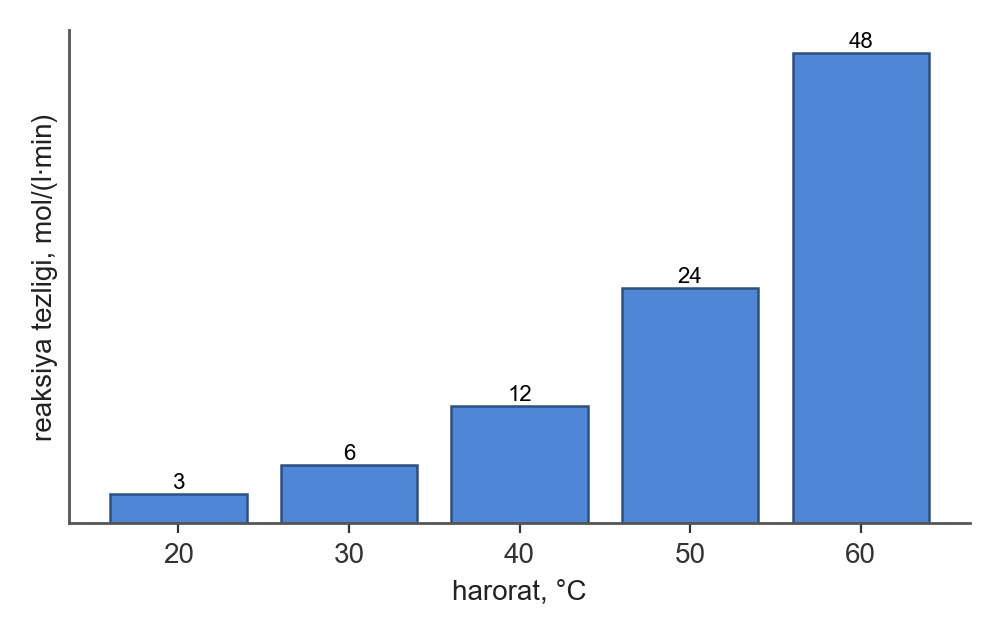
\includegraphics[width=0.86\linewidth]{rasmlar/gen/vh_v13_0.png}\end{center}
Haroratni 20 \textdegree{}C dan 50 \textdegree{}C gacha ko`tarilganda tezlik necha marta ortadi?

\noindent A)~\textsl{8} \hfill B)~\textsl{6} \hfill C)~\textsl{16} \hfill D)~\textsl{4}\par
\qsep
\noindent\qn{2.} CO + Cl\textsubscript{2} $\rightleftarrows$ COCl\textsubscript{2} reaksiyasi 5 l hajmli idishda o`tkazildi. Ma'lumotlar jadvalda berilgan:
\begin{center}
\renewcommand{\arraystretch}{1.15}
\fitbox{\begin{tabular}{|c|c|c|c|}\hline
\textbf{Modda} & \textbf{CO} & \textbf{Cl\textsubscript{2}} & \textbf{COCl\textsubscript{2}} \\ \hline
Boshlang`ich, mol & 6 & 3 & 0 \\ \hline
Muvozanatda, mol & --- & --- & 1 \\ \hline
\end{tabular}}
\end{center}
Muvozanat \textbf{konstantasini (K) hisoblang.}

\noindent A)~\textsl{1} \hfill B)~\textsl{0,5} \hfill C)~\textsl{0,25} \hfill D)~\textsl{2,5}\par
\qsep
\noindent\qn{3.} N\textsubscript{2} + 3H\textsubscript{2} $\rightleftarrows$ 2NH\textsubscript{3} reaksiyasida N\textsubscript{2} va H\textsubscript{2} stexiometrik nisbatda olingan umumiy 20 mol aralashma muvozanat qaror topganda doimiy T va \textit{V} da bosim 25\% ga kamaydi. Muvozanatdagi NH\textsubscript{3} ning \textbf{miqdorini (mol) aniqlang.}

\noindent A)~\textsl{5} \hfill B)~\textsl{2,5} \hfill C)~\textsl{7,5} \hfill D)~\textsl{10}\par
\qsep
\noindent\qn{4.} Qaysi juftliklarda reaksiya boradi? 1) Cu va ZnSO\textsubscript{4}; 2) Fe va CuCl\textsubscript{2}; 3) Ag va CuSO\textsubscript{4}; 4) Zn va CuSO\textsubscript{4}

\noindent A)~\textsl{2, 4} \hfill B)~\textsl{1, 2, 3} \hfill C)~\textsl{2} \hfill D)~\textsl{3}\par
\qsep
\noindent\qn{5.} 12 g NaOH ni to`liq neytrallash uchun 18,9 g HNO\textsubscript{3} sarflandi. HNO\textsubscript{3} ning ekvivalent \textbf{massasini (g/mol) aniqlang.}

\noindent A)~\textsl{126} \hfill B)~\textsl{31,5} \hfill C)~\textsl{18,9} \hfill D)~\textsl{63}\par
\qsep
\noindent\qn{6.} AgNO\textsubscript{3} eritmasi inert elektrodlar yordamida 2 A tok kuchi bilan 965 s elektroliz qilindi. Katodda ajralgan Ag massasi (g) \textbf{ni toping.}

\noindent A)~\textsl{2,16} \hfill B)~\textsl{4,32} \hfill C)~\textsl{1,08} \hfill D)~\textsl{0,043}\par
\qsep
\noindent\qn{7.} Xlor (\textit{Z} = 17) atomining tashqi energetik pog`onasidagi elektronlar \textbf{sonini aniqlang.}

\noindent A)~\textsl{7} \hfill B)~\textsl{8} \hfill C)~\textsl{6} \hfill D)~\textsl{9}\par
\qsep
\noindent\qn{8.} Quyidagi tuzlarning qaysilari suvli eritmasi kislotali muhitga ega? 1) ZnCl\textsubscript{2}; 2) NH\textsubscript{4}Cl; 3) CH\textsubscript{3}COONa; 4) Na\textsubscript{2}CO\textsubscript{3}

\noindent A)~\textsl{1, 4} \hfill B)~\textsl{1, 2} \hfill C)~\textsl{3} \hfill D)~\textsl{4}\par
\qsep
\noindent\qn{9.} Laboratoriyada NH\textsubscript{4}NO\textsubscript{3} eritmalari quyidagicha tayyorlangan:
\begin{center}
\renewcommand{\arraystretch}{1.15}
\fitbox{\begin{tabular}{|c|c|c|}\hline
\textbf{Idish} & \textbf{Eritma massasi, g} & \textbf{$\omega$(NH\textsubscript{4}NO\textsubscript{3}), \%} \\ \hline
A & 200 & 5 \\ \hline
B & 300 & 40 \\ \hline
\end{tabular}}
\end{center}
Bu ikki eritma bir idishga quyilib va ustiga 100 g suv qo`shilsa, yangi eritmadagi NH\textsubscript{4}NO\textsubscript{3} ning massa ulushi (\%) qancha bo`ladi?

\noindent A)~\textsl{22,5} \hfill B)~\textsl{21,67} \hfill C)~\textsl{45} \hfill D)~\textsl{19}\par
\qsep
\noindent\qn{10.} CO\textsubscript{2} gazining 27 \textdegree{}C va 4 atm bosimdagi \textbf{zichligini (g/l) aniqlang.} (R = 0,082 l$\cdot$atm/(mol$\cdot$K))

\noindent A)~\textsl{14,31} \hfill B)~\textsl{7,15} \hfill C)~\textsl{3,58} \hfill D)~\textsl{1,96}\par
\qsep
\noindent\qn{11.} HC$\equiv$C--CH=CH\textsubscript{2} molekulasida sp\textsuperscript{2} gibridlangan uglerod atomlari nechta?

\noindent A)~\textsl{3} \hfill B)~\textsl{4} \hfill C)~\textsl{1} \hfill D)~\textsl{2}\par
\qsep
\noindent\qn{12.} NaCl ning suvli eritmasi inert elektrodlar bilan elektroliz qilinganda qaysi moddalar ajraladi?

\noindent\begin{tabular}{@{}p{0.47\linewidth}@{}p{0.47\linewidth}@{}}
A)~\textsl{Zn, H\textsubscript{2} va O\textsubscript{2}} & B)~\textsl{H\textsubscript{2}, Cl\textsubscript{2} va NaOH} \\
C)~\textsl{H\textsubscript{2} va O\textsubscript{2}} & D)~\textsl{Ag va O\textsubscript{2}} \\
\end{tabular}\par
\qsep
\noindent\qn{13.} Tabiiy elementning ikki izotopi: \textsuperscript{63}Cu (70\%) va \textsuperscript{65}Cu (30\%). Elementning o`rtacha nisbiy atom \textbf{massasini aniqlang.}

\noindent A)~\textsl{63,6} \hfill B)~\textsl{64} \hfill C)~\textsl{64,4} \hfill D)~\textsl{63}\par
\qsep
\noindent\qn{14.} 2Mg + CO\textsubscript{2} $\to$ 2MgO + C reaksiyasida 4,4 g CO\textsubscript{2} ishtirok etdi. C \textbf{miqdorini (mol) toping.}

\noindent A)~\textsl{0,2} \hfill B)~\textsl{0,05} \hfill C)~\textsl{0,15} \hfill D)~\textsl{0,1}\par
\qsep
\noindent\qn{15.} Reaksiya tenglamasi: H\textsubscript{2} + Cl\textsubscript{2} $\to$ 2HCl. Reaksiyaga 0,5 g H\textsubscript{2} kirishdi. HCl \textbf{hajmini (l, n.sh.) hisoblang.}

\noindent A)~\textsl{2,8} \hfill B)~\textsl{22,4} \hfill C)~\textsl{11,2} \hfill D)~\textsl{5,6}\par
\qsep
\noindent\qn{16.} Ishqoriy metallar haqida qaysi fikrlar to`g`ri? 1) Litiy eng yengil metall; 2) Natriy suv bilan reaksiyada H\textsubscript{2} va NaOH hosil qiladi; 3) Natriyning olinishi suyuqlanma NaCl elektrolizi bilan; 4) Natriy atomining tashqi qavatida 2 ta elektron bor

\noindent A)~\textsl{1, 2, 3} \hfill B)~\textsl{1, 3} \hfill C)~\textsl{1, 4} \hfill D)~\textsl{1, 2}\par
\qsep
\noindent\qn{17.} Alyuminiy va magniy dan iborat 10,5 g aralashma mo`l NaOH eritmasida eritildi. Ajralgan gazning \textbf{hajmini (l, n.sh.) aniqlang} (magniy ishqor bilan reaksiyaga kirishmaydi).

\noindent A)~\textsl{20,16} \hfill B)~\textsl{5,04} \hfill C)~\textsl{8,71} \hfill D)~\textsl{10,08}\par
\qsep
\noindent\qn{18.} D-metallar va ularning birikmalari haqida qaysi fikrlar to`g`ri? 1) Fe(OH)\textsubscript{2} havoda qo`ng`ir rangga o`tadi; 2) Zn(OH)\textsubscript{2} amfoter xossaga ega; 3) Mis nam havoda (CuOH)\textsubscript{2}CO\textsubscript{3} qoplamasi bilan qoplanadi; 4) Temir sovuq konsentrlangan HNO\textsubscript{3} da passivlanadi

\noindent\begin{tabular}{@{}p{0.47\linewidth}@{}p{0.47\linewidth}@{}}
A)~\textsl{1, 2, 4} & B)~\textsl{1, 3, 4} \\
C)~\textsl{1, 2, 3, 4} & D)~\textsl{2, 3, 4} \\
\end{tabular}\par
\qsep
\noindent\qn{19.} Reaksiya tenglamasi: MgCl\textsubscript{2} + Na\textsubscript{2}CO\textsubscript{3} $\to$ MgCO\textsubscript{3} + 2NaCl. Reaksiyaga 47,5 g MgCl\textsubscript{2} kirishdi. MgCO\textsubscript{3} \textbf{massasini (g) hisoblang.}

\noindent A)~\textsl{84} \hfill B)~\textsl{21} \hfill C)~\textsl{42} \hfill D)~\textsl{63}\par
\qsep
\noindent\qn{20.} Alkanlar va sikloalkanlar haqida qaysi fikrlar to`g`ri? 1) Sikloalkanlarning umumiy formulasi CnH\textsubscript{2}n; 2) Metanning katalitik oksidlanishidan formaldegid olinadi; 3) Metan suvda yaxshi eriydi; 4) Propan odatiy sharoitda gaz

\noindent A)~\textsl{1, 3, 4} \hfill B)~\textsl{1, 3} \hfill C)~\textsl{1, 2, 4} \hfill D)~\textsl{2, 4}\par
\qsep
\noindent\qn{21.} CH\textsubscript{3}--CH(CH\textsubscript{3})--CH\textsubscript{2}--OH birikmaning sistematik nomi qaysi qatorda to`g`ri keltirilgan?

\noindent\begin{tabular}{@{}p{0.47\linewidth}@{}p{0.47\linewidth}@{}}
A)~\textsl{butanol-1} & B)~\textsl{2-metilpropanol-2} \\
C)~\textsl{butanol-2} & D)~\textsl{2-metilpropanol-1} \\
\end{tabular}\par
\qsep
\noindent\qn{22.} Arenlar, neft va tabiiy gaz haqida qaysi fikrlar to`g`ri? 1) Benzol bromli suvni rangsizlantirmaydi; 2) Naftalin -- bir halqali aren; 3) Toluol KMnO\textsubscript{4} bilan benzoy kislotagacha oksidlanadi; 4) Neft fraksiyalaridan gazolin 150 \textdegree{}C gacha haydaladi

\noindent A)~\textsl{1, 3, 4} \hfill B)~\textsl{2, 4} \hfill C)~\textsl{1, 3} \hfill D)~\textsl{2, 3, 4}\par
\qsep
\noindent\qn{23.} Rasmda tasvirlangan molekuladagi sp\textsuperscript{3}-gibridlangan uglerod atomlari \textbf{sonini aniqlang.}
\begin{center}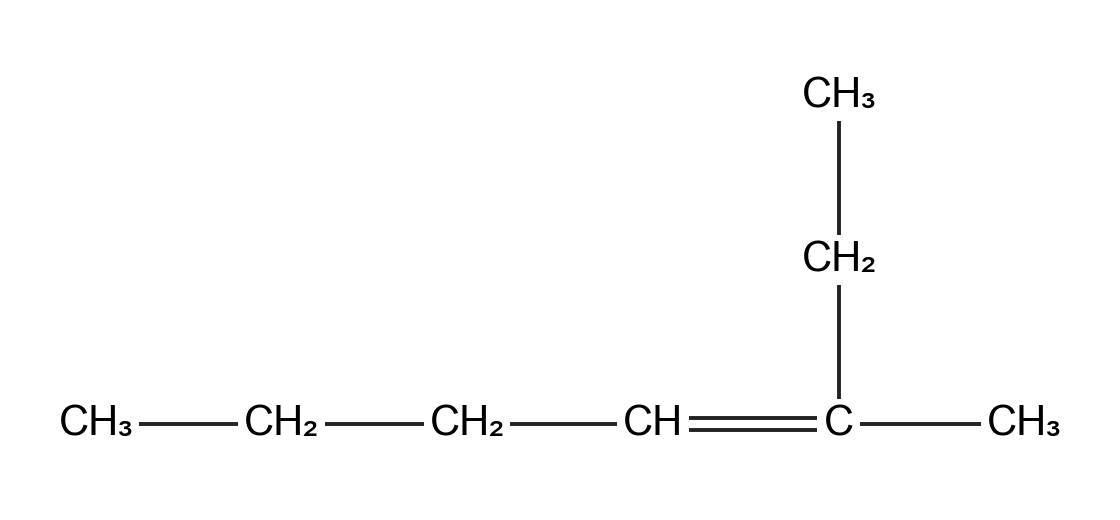
\includegraphics[width=0.86\linewidth]{rasmlar/gen/struct_16944700_887.png}\end{center}

\noindent A)~\textsl{7} \hfill B)~\textsl{5} \hfill C)~\textsl{8} \hfill D)~\textsl{6}\par
\qsep
\noindent\qn{24.} CH\textsubscript{3}CHO + H\textsubscript{2} $\to$ C\textsubscript{2}H\textsubscript{5}OH reaksiyasida 22,4 l (n.sh.) H\textsubscript{2} ishtirok etdi. C\textsubscript{2}H\textsubscript{5}OH \textbf{massasini (g) toping.}

\noindent A)~\textsl{92} \hfill B)~\textsl{23} \hfill C)~\textsl{69} \hfill D)~\textsl{46}\par
\qsep
\noindent\qn{25.} Reaksiya tenglamasi: CH\textsubscript{3}COOH + NaHCO\textsubscript{3} $\to$ CH\textsubscript{3}COONa + CO\textsubscript{2} + H\textsubscript{2}O. Reaksiyaga 12 g CH\textsubscript{3}COOH kirishdi. CO\textsubscript{2} \textbf{hajmini (l, n.sh.) hisoblang.}

\noindent A)~\textsl{8,96} \hfill B)~\textsl{2,24} \hfill C)~\textsl{6,72} \hfill D)~\textsl{4,48}\par
\qsep
\noindent\qn{26.} Murakkab efirlar va yog`lar haqida qaysi fikrlar to`g`ri? 1) Etilatsetat efir hidli suyuqlik; 2) Suyuq yog`larni gidrogenlab qattiq yog` olinadi; 3) Murakkab efirlarning gidrolizi ishqoriy muhitda qaytmas; 4) Yog`lar glitserin va yuqori yog` kislotalarning murakkab efirlari

\noindent\begin{tabular}{@{}p{0.47\linewidth}@{}p{0.47\linewidth}@{}}
A)~\textsl{1, 2, 4} & B)~\textsl{2, 3, 4} \\
C)~\textsl{1, 2, 3, 4} & D)~\textsl{1, 2, 3} \\
\end{tabular}\par
\qsep
\noindent\qn{27.} 1 mol glyukoza spirtli bijg`itilganda hosil bo`lgan etanol \textbf{massasini (g) aniqlang.}

\noindent A)~\textsl{46} \hfill B)~\textsl{184} \hfill C)~\textsl{92} \hfill D)~\textsl{180}\par
\qsep
\noindent\qn{28.} Aminlar, aminokislotalar va oqsillar haqida qaysi fikrlar to`g`ri? 1) Oqsillar biuret reaksiyasini beradi; 2) Nitrobenzoldan anilin Zinin reaksiyasi bilan olinadi; 3) Dipeptidda 2 ta peptid bog` bor; 4) Aminokislotalar faqat kislotali xossaga ega

\noindent A)~\textsl{1, 3, 4} \hfill B)~\textsl{1, 2} \hfill C)~\textsl{1, 3} \hfill D)~\textsl{2, 4}\par
\qsep
\noindent\qn{29.} 2,6 g C\textsubscript{2}H\textsubscript{2} dan quyidagi ikki bosqichda C\textsubscript{2}H\textsubscript{5}OH olinadi: 1) C\textsubscript{2}H\textsubscript{2} + H\textsubscript{2} $\to$ C\textsubscript{2}H\textsubscript{4} (unum 80\%); 2) C\textsubscript{2}H\textsubscript{4} + H\textsubscript{2}O $\to$ C\textsubscript{2}H\textsubscript{5}OH (unum 50\%). Oxirgi mahsulot C\textsubscript{2}H\textsubscript{5}OH ning \textbf{massasini (g) toping.}

\noindent A)~\textsl{2,3} \hfill B)~\textsl{3,68} \hfill C)~\textsl{1,84} \hfill D)~\textsl{4,6}\par
\qsep
\noindent\qn{30.} Kimyo laboratoriyasida ishlash qoidalari haqida qaysi fikrlar to`g`ri? 1) Ishqor teriga tushsa, qo`l suv bilan yuviladi; 2) Zaharli gaz ajraladigan tajriba mo`rili shkafda o`tkaziladi; 3) Spirt lampa boshqa lampadan yoqilmaydi; 4) Konsentrlangan kislotani suvga ohista, aralashtirib quyiladi

\noindent\begin{tabular}{@{}p{0.47\linewidth}@{}p{0.47\linewidth}@{}}
A)~\textsl{1, 2, 3} & B)~\textsl{1, 2, 3, 4} \\
C)~\textsl{1, 3, 4} & D)~\textsl{2, 3, 4} \\
\end{tabular}\par
\qsep
\noindent\qn{31.} Quyidagi aralashmani ajratish uchun qaysi usul mos: osh tuzi eritmasidan tuz?
\noindent A)~\textsl{sublimatsiya (yod haydaladi)}\par
\noindent B)~\textsl{bug`latish}\par
\noindent C)~\textsl{magnit yordamida ajratish (temir tortiladi)}\par
\noindent D)~\textsl{filtrlash}\par
\qsep
\noindent\qn{32.} Rasmdagi usul bilan qaysi aralashmani ajratish mumkin?
\begin{center}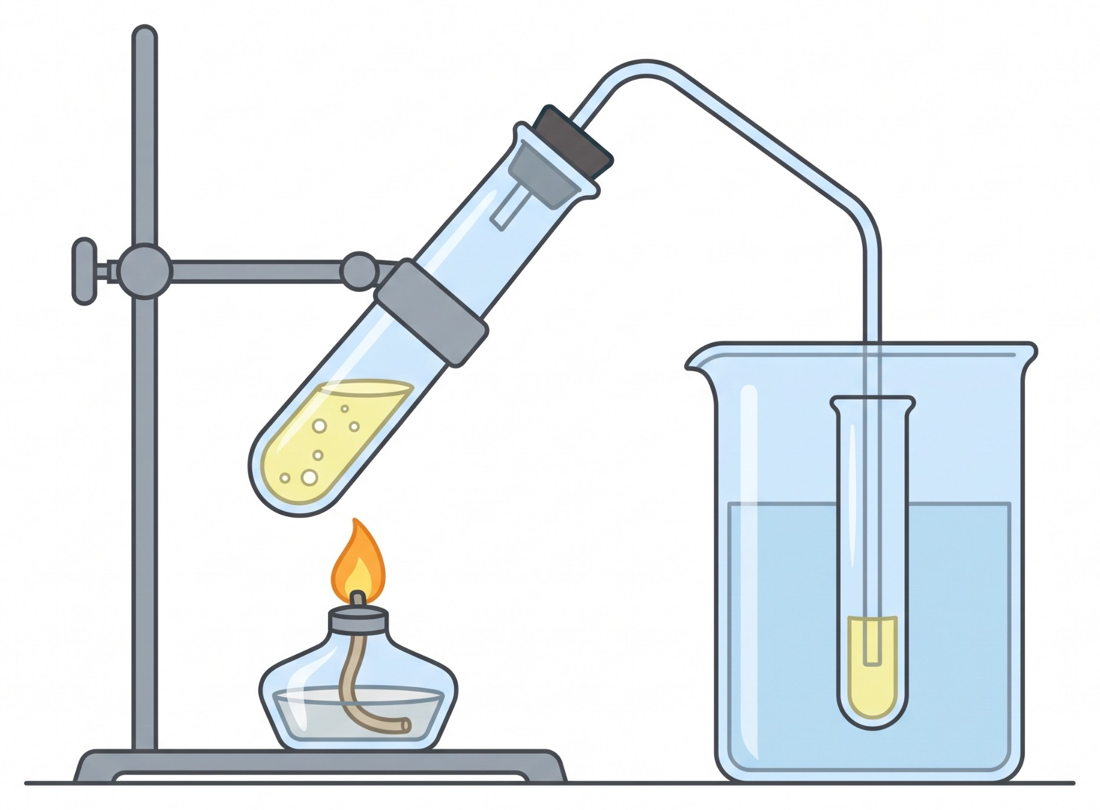
\includegraphics[width=0.86\linewidth]{rasmlar/darslik/d_distill.png}\end{center}

\noindent\begin{tabular}{@{}p{0.47\linewidth}@{}p{0.47\linewidth}@{}}
A)~\textsl{osh tuzi va qum} & B)~\textsl{suv va qum} \\
C)~\textsl{suv va etanol} & D)~\textsl{suv va kerosin   ---} \\
\end{tabular}\par
\qsep
\end{multicols}
\medskip
\noindent\setlength{\fboxsep}{0pt}\fbox{\begin{tabular}{p{0.74\linewidth}|p{0.2\linewidth}}
\parbox[t]{0.72\linewidth}{\vspace{3pt}\textbf{Topshiriqlar (33--35) va javob variant (A--F)larini o`zaro to`g`ri moslashtiring.} NaBr va KI dan iborat 28,9 g aralashma suvda eritilib, mo`l AgNO\textsubscript{3} eritmasi qo`shildi; hosil bo`lgan cho`kmalarning umumiy massasi 49,35 g.
\vspace{3pt}} & \parbox[t]{0.19\linewidth}{\vspace{3pt}A~\textsl{850}\\[3pt]
B~\textsl{20,6}\\[3pt]
C~\textsl{16,48}\\[3pt]
D~\textsl{22,05}\\[3pt]
E~\textsl{425}\\[3pt]
F~\textsl{11,03}}\\ \hline
\parbox[t]{0.72\linewidth}{\vspace{2pt}\textbf{33. Aralashmadagi NaBr massasini (g) aniqlang.}\vspace{2pt}} & \\ \hline
\parbox[t]{0.72\linewidth}{\vspace{2pt}\textbf{34. Sarflangan 10\% li AgNO\textsubscript{3} eritmasining massasini (g) aniqlang (M(AgNO\textsubscript{3}) = 170 g/mol).}\vspace{2pt}} & \\ \hline
\parbox[t]{0.72\linewidth}{\vspace{2pt}\textbf{35. Eritmada hosil bo`lgan nitratlarning umumiy massasini (g) aniqlang.}\vspace{2pt}} & 
\end{tabular}}
\par\bigskip
\noindent\qn{36.} C + HNO\textsubscript{3} $\to$ CO\textsubscript{2} + NO\textsubscript{2} + H\textsubscript{2}O reaksiya tenglamasini tenglang. Reagentlar (chap qism) koeffitsiyentlari \textbf{yig`indisini toping.}
\javob\qsep
\noindent\qn{37.} 2NO + O\textsubscript{2} $\rightleftarrows$ 2NO\textsubscript{2} reaksiyada muvozanat holatida [NO] = 1, [O\textsubscript{2}] = 1, [NO\textsubscript{2}] = 1 mol/l. Muvozanat \textbf{konstantasini (K) hisoblang.}
\javob\qsep
\noindent\qn{38.} Alyuminiy (0,1 mol) va kalsiy (0,1 mol) aralashmasi mo`l xlorid kislotada eritildi. Ajralgan vodorodning \textbf{hajmini (l, n.sh.) aniqlang.}
\javob\qsep
\noindent\qn{39.} 180 g glyukoza spirtli bijg`ish natijasida etanolga (unum 80\%), hosil bo`lgan etanol esa sirka kislotagacha (unum 80\%) aylantirildi. Olingan kislotani to`liq neytrallash uchun NaOH ning \textbf{massasini (g) toping.}
\javob\qsep
\noindent\qn{40.} 17,8 g tristearin mo`l NaOH eritmasi bilan to`liq gidrolizlandi (sovun unumi 80\%). Hosil bo`lgan natriy stearat (M = 306 g/mol) \textbf{massasini (g) toping.}
\javob\qsep
\par\bigskip\begin{center}\textbf{\fontsize{13}{15}\selectfont YOZMA ISH}\end{center}
\noindent\qn{41.} \textbf{Topshiriqni bajarish jarayonida barcha reaksiya tenglamalarini yozing. Miqdoriy va arifmetik hisoblashlarni (unga asos bo`lgan usul yoki formulani ko`rsatgan holda) uzviy ketma-ketlikda bajaring.}\par\smallskip
Hajmi 2 l bo`lgan idishda 2NO + O\textsubscript{2} $\rightleftarrows$ 2NO\textsubscript{2} sistema muvozanat holatiga keldi. Muvozanat qaror topganda idishdagi moddalar miqdori: NO -- 2 mol, O\textsubscript{2} -- 0,5 mol; NO\textsubscript{2} -- 1 mol.\par
\noindent 1)\ Muvozanat konstantasini (K) hisoblang.\par
\noindent 2)\ Moddalarning boshlang`ich konsentratsiyalarini (mol/l) aniqlang. Boshlang`ich moddalarning umumiy miqdorini (mol) ham toping.\par
\noindent 3)\ NO ning necha foizi reaksiyaga kirishgan?\par
\noindent 4)\ Idish hajmi izotermik ravishda 2 marta kamaytirilsa, to`g`ri reaksiya tezligi (elementar reaksiya deb hisoblang) necha marta o`zgaradi? Teskari reaksiya uchun K' = 1/K ni ham hisoblang.\par
\noindent 5)\ Bosim oshirilganda muvozanat qaysi tomonga siljiydi va K qiymati qanday o`zgaradi? Muvozanatdagi umumiy mol miqdorining boshlang`ich mol miqdoriga nisbatini toping. Muvozanat aralashmasining o`rtacha molyar massasini (g/mol) ham hisoblang.\par
\diqqat{Mazkur topshiriq kengaytirilgan javobni talab etib, uning yechilish usuli va shu usul asosidagi barcha hisoblash amallari javoblar varaqasida aks etishi lozim.}\qsep
\noindent\qn{42.} Quyidagi o`zgarishlar zanjirida \textit{X}, \textit{Y}, \textit{Z} noma'lum organik moddalar:\par
\[\setlength{\fboxsep}{0pt}\text{CH\textsubscript{3}CHO}\xrightarrow{\text{H\textsubscript{2}, Ni}}\text{\textit{X}}\xrightarrow{\text{H\textsubscript{2}SO\textsubscript{4} (kons.), 170 \textdegree{}C}}\text{\textit{Y}}\xrightarrow{\text{Br\textsubscript{2}}}\text{C\textsubscript{2}H\textsubscript{4}Br\textsubscript{2}}\]
\noindent 1)\ CH\textsubscript{3}CHO $\to$ \textit{X} : reaksiya tenglamasini yozing; hosil bo`lgan moddani nomlang.\par
\noindent 2)\ \textit{X} $\to$ \textit{Y} : reaksiya tenglamasini yozing; hosil bo`lgan moddani nomlang.\par
\noindent 3)\ \textit{Y} $\to$ C\textsubscript{2}H\textsubscript{4}Br\textsubscript{2} : reaksiya tenglamasini yozing; hosil bo`lgan moddani nomlang.\par
\diqqat{Mazkur topshiriq kengaytirilgan javobni talab etib, uning yechilish usuli va shu usul asosidagi barcha hisoblash amallari javoblar varaqasida aks etishi lozim.}\qsep
\noindent\qn{43.} \textbf{Topshiriqni bajarish jarayonida barcha reaksiya tenglamalarini yozing. Miqdoriy va arifmetik hisoblashlarni (unga asos bo`lgan usul yoki formulani ko`rsatgan holda) uzviy ketma-ketlikda bajaring.}\par\smallskip
60 g pirit (FeS\textsubscript{2}) yondirildi: 4FeS\textsubscript{2} + 11O\textsubscript{2} $\to$ 2Fe\textsubscript{2}O\textsubscript{3} + 8SO\textsubscript{2} (unum 100\%). Hosil bo`lgan SO\textsubscript{2} katalizator ishtirokida SO\textsubscript{3} gacha oksidlandi (unum 80\%), SO\textsubscript{3} suvda eritildi.\par
\noindent 1)\ Hosil bo`lgan SO\textsubscript{2} hajmini (l, n.sh.) va qattiq qoldiq Fe\textsubscript{2}O\textsubscript{3} massasini (g) hisoblang. Shuningdek SO\textsubscript{2} massasini (g) ham toping.\par
\noindent 2)\ SO\textsubscript{3} ning massasini (g) toping (2SO\textsubscript{2} + O\textsubscript{2} $\rightleftarrows$ 2SO\textsubscript{3}).\par
\noindent 3)\ Hosil bo`lgan H\textsubscript{2}SO\textsubscript{4} massasini (g) aniqlang.\par
\noindent 4)\ Shu kislotani to`liq neytrallash uchun zarur NaOH massasini (g) va mo`l BaCl\textsubscript{2} bilan hosil bo`ladigan cho`kma massasini (g) toping.\par
\noindent 5)\ Shu H\textsubscript{2}SO\textsubscript{4} dan 20\% li eritma tayyorlash uchun qancha suv (g) kerak?\par
\diqqat{Mazkur topshiriq kengaytirilgan javobni talab etib, uning yechilish usuli va shu usul asosidagi barcha hisoblash amallari javoblar varaqasida aks etishi lozim.}\qsep
\newpage
\renewcommand{\curvar}{14-variant}
\thispagestyle{first}
\noindent\textit{Davriy jadvaldan foydalanish mumkin.}
\par\smallskip
\begin{multicols}{2}
\noindent\qn{1.} Mis (\textit{Z} = 29) atomida nechta juftlashmagan elektron bor?

\noindent A)~\textsl{2} \hfill B)~\textsl{3} \hfill C)~\textsl{1} \hfill D)~\textsl{0}\par
\qsep
\noindent\qn{2.} 12 g NaOH ni to`liq neytrallash uchun 10,95 g HCl sarflandi. HCl ning ekvivalent \textbf{massasini (g/mol) aniqlang.}

\noindent A)~\textsl{73} \hfill B)~\textsl{36,5} \hfill C)~\textsl{18,25} \hfill D)~\textsl{10,95}\par
\qsep
\noindent\qn{3.} Jadvalda metall plastinkalarning tuz eritmalariga tushirilishidagi kuzatuvlar berilgan (``+'' -- metall ajraladi, reaksiya boradi; ``$-$'' -- reaksiya bormaydi):
\begin{center}
\renewcommand{\arraystretch}{1.15}
\fitbox{\begin{tabular}{|c|c|c|c|}\hline
\textbf{Metall} & \textbf{ZnSO\textsubscript{4} eritmasi} & \textbf{MgSO\textsubscript{4} eritmasi} & \textbf{CuSO\textsubscript{4} eritmasi} \\ \hline
Fe & $-$ & $-$ & + \\ \hline
Zn & $-$ & $-$ & + \\ \hline
Mg & + & $-$ & + \\ \hline
\end{tabular}}
\end{center}
Ushbu metallardan qaysi biri eng faol?

\noindent A)~\textsl{Fe} \hfill B)~\textsl{Zn} \hfill C)~\textsl{Mg} \hfill D)~\textsl{Cu}\par
\qsep
\noindent\qn{4.} 26,24 l Cl\textsubscript{2} 127 \textdegree{}C va 0,5 atm bosimda necha gramm keladi? (R = 0,082 l$\cdot$atm/(mol$\cdot$K))

\noindent A)~\textsl{56,8} \hfill B)~\textsl{28,4} \hfill C)~\textsl{14,2} \hfill D)~\textsl{83,17}\par
\qsep
\noindent\qn{5.} Rasmda Li va F atomlari orasida elektron o`tishi sxematik ko`rsatilgan (ion bog` hosil bo`lishi).
\begin{center}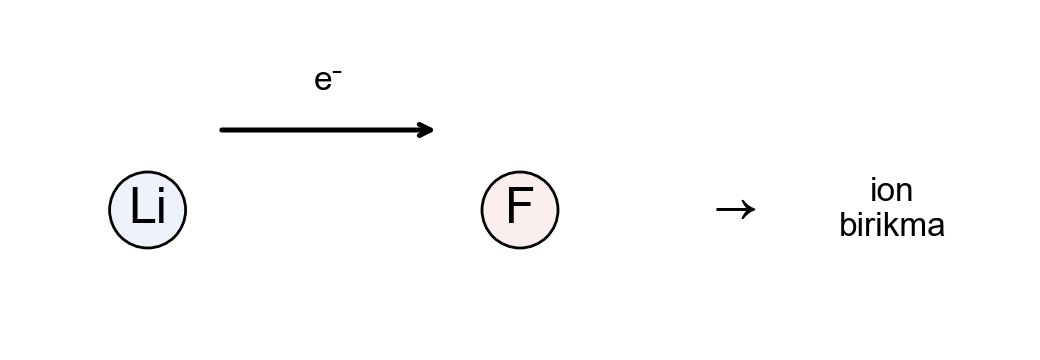
\includegraphics[width=0.86\linewidth]{rasmlar/gen/ib_889354.png}\end{center}
Li atomi qancha elektron berib, qanday zaryadli ionga aylanadi?

\noindent A)~\textsl{1 ta, $-$1} \hfill B)~\textsl{2 ta, +2} \hfill C)~\textsl{3 ta, +3} \hfill D)~\textsl{1 ta, +1}\par
\qsep
\noindent\qn{6.} AgNO\textsubscript{3} ning suvli eritmasi inert elektrodlar bilan elektroliz qilinganda qaysi moddalar ajraladi?

\noindent\begin{tabular}{@{}p{0.47\linewidth}@{}p{0.47\linewidth}@{}}
A)~\textsl{Ag va O\textsubscript{2}} & B)~\textsl{Zn, H\textsubscript{2} va O\textsubscript{2}} \\
C)~\textsl{H\textsubscript{2} va O\textsubscript{2}} & D)~\textsl{H\textsubscript{2}, Cl\textsubscript{2} va NaOH} \\
\end{tabular}\par
\qsep
\noindent\qn{7.} Reaksiya tezligining haroratga bog`liqligi jadvalda berilgan:
\begin{center}
\renewcommand{\arraystretch}{1.15}
\fitbox{\begin{tabular}{|c|c|c|c|}\hline
\textbf{T, \textdegree{}C} & \textbf{20} & \textbf{30} & \textbf{40} \\ \hline
v, mol/(l$\cdot$s) & 0,5 & 1,5 & 4,5 \\ \hline
\end{tabular}}
\end{center}
Jadvaldan foydalanib, shu reaksiyaning 60 \textdegree{}C dagi tezligini (mol/(l$\cdot$s)) \textbf{aniqlang.}

\noindent A)~\textsl{40,5} \hfill B)~\textsl{13,5} \hfill C)~\textsl{121,5} \hfill D)~\textsl{81}\par
\qsep
\noindent\qn{8.} Quyidagi jadvalda BaCl\textsubscript{2} tuzining eritmalari keltirilgan:
\begin{center}
\renewcommand{\arraystretch}{1.15}
\fitbox{\begin{tabular}{|c|c|c|}\hline
\textbf{No.} & \textbf{m(eritma), g} & \textbf{$\omega$, \%} \\ \hline
I & 200 & 10 \\ \hline
II & 200 & 30 \\ \hline
\end{tabular}}
\end{center}
Eritmalar aralashtirilib, ustiga 50 g suv qo`shildi. Oxirgi eritmadagi tuzning massa \textbf{ulushini (\%) toping.}

\noindent A)~\textsl{20} \hfill B)~\textsl{40} \hfill C)~\textsl{17,78} \hfill D)~\textsl{16}\par
\qsep
\noindent\qn{9.} Jadvalda bog`lar hosil qiluvchi atomlarning elektrmanfiyliklari berilgan:
\begin{center}
\renewcommand{\arraystretch}{1.15}
\fitbox{\begin{tabular}{|c|c|c|}\hline
\textbf{Bog`} & \textbf{EM (1-atom)} & \textbf{EM (2-atom)} \\ \hline
Al--Cl & 1,5 & 3 \\ \hline
Si--O & 1,8 & 3,5 \\ \hline
H--O & 2,1 & 3,5 \\ \hline
H--Cl & 2,1 & 3 \\ \hline
\end{tabular}}
\end{center}
Qaysi bog` eng qutbli (eng ko`p ionli xarakterga ega)?

\noindent A)~\textsl{Al--Cl} \hfill B)~\textsl{H--O} \hfill C)~\textsl{H--Cl} \hfill D)~\textsl{Si--O}\par
\qsep
\noindent\qn{10.} Xrom (\textit{Z} = 24) atomi elektron konfiguratsiyasida jami nechta juftlashgan elektron bor?

\noindent A)~\textsl{19} \hfill B)~\textsl{18} \hfill C)~\textsl{17} \hfill D)~\textsl{20}\par
\qsep
\noindent\qn{11.} He va O\textsubscript{2} gazlari 2 : 1 hajmiy nisbatda aralashtirildi. Aralashmaning vodorodga nisbatan \textbf{zichligini aniqlang.}

\noindent A)~\textsl{6,67} \hfill B)~\textsl{13,33} \hfill C)~\textsl{7,67} \hfill D)~\textsl{9}\par
\qsep
\noindent\qn{12.} Gazlar aralashmasi tarkibi jadvalda berilgan (n.sh.):
\begin{center}
\renewcommand{\arraystretch}{1.15}
\fitbox{\begin{tabular}{|c|c|}\hline
\textbf{Gaz} & \textbf{Hajmi, l} \\ \hline
O\textsubscript{2} & 2 \\ \hline
NH\textsubscript{3} & 2 \\ \hline
N\textsubscript{2} & 2 \\ \hline
\end{tabular}}
\end{center}
Aralashmaning havoga nisbatan \textbf{zichligini aniqlang} (M(havo) = 29 g/mol).

\noindent A)~\textsl{1,77} \hfill B)~\textsl{0,44} \hfill C)~\textsl{0,89} \hfill D)~\textsl{25,67}\par
\qsep
\noindent\qn{13.} 25 ml HCl eritmasi 0,05 mol/l li NaOH eritmasi bilan titrlandi. Titrlash egri chizig`i grafikda berilgan (ekvivalent nuqta 25 ml da).
\begin{center}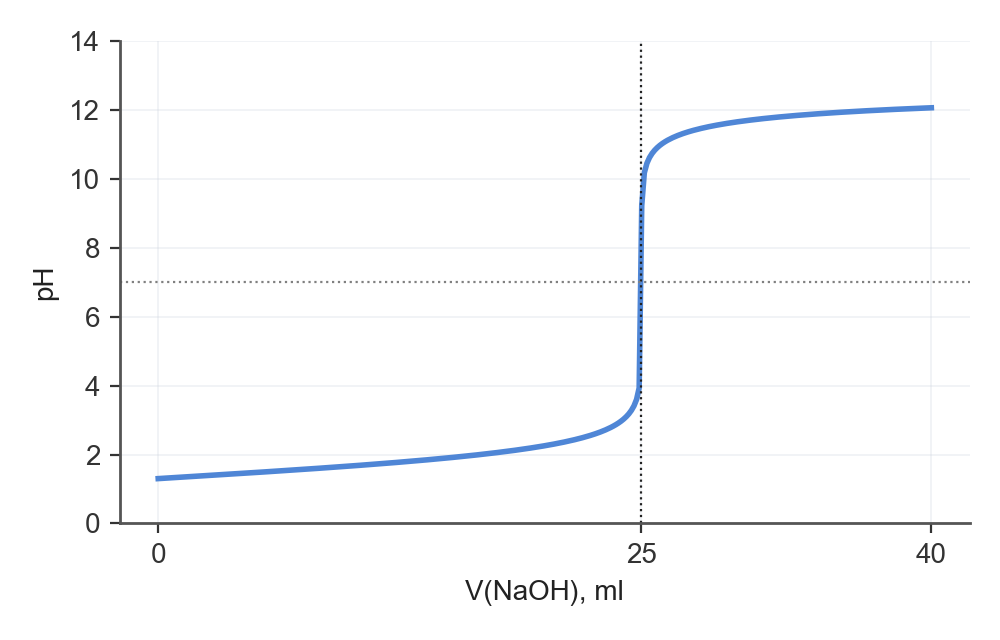
\includegraphics[width=0.86\linewidth]{rasmlar/gen/ti_v14_0.png}\end{center}
Grafikning boshlang`ich nuqtasi (\textit{V} = 0) pH ining qiymatiga mos keluvchi HCl eritmasidagi H\textsuperscript{+} \textbf{konsentratsiyasini (mol/l) toping.}

\noindent A)~\textsl{0,5} \hfill B)~\textsl{0,005} \hfill C)~\textsl{0,1} \hfill D)~\textsl{0,05}\par
\qsep
\noindent\qn{14.} K va Li dan iborat 13,1 g aralashma suv bilan reaksiyaga kirishdi. Ajralgan vodorodning \textbf{hajmini (l, n.sh.) aniqlang.}

\noindent A)~\textsl{11,2} \hfill B)~\textsl{2,8} \hfill C)~\textsl{6,55} \hfill D)~\textsl{5,6}\par
\qsep
\noindent\qn{15.} Alyuminiy va temir dan iborat 19,3 g aralashma mo`l NaOH eritmasida eritilganda 10,08 l (n.sh.) gaz ajraldi. Aralashmadagi temir ning massa \textbf{ulushini (\%) aniqlang.}

\noindent A)~\textsl{42} \hfill B)~\textsl{29} \hfill C)~\textsl{58} \hfill D)~\textsl{37,8}\par
\qsep
\noindent\qn{16.} D-metallar va ularning birikmalari haqida qaysi fikrlar to`g`ri? 1) Mis suyultirilgan HCl bilan reaksiyaga kirishadi; 2) Fe(OH)\textsubscript{2} havoda qo`ng`ir rangga o`tadi; 3) Xrom (VI) oksidi (CrO\textsubscript{3}) kislotali oksid; 4) Temirning Cl\textsubscript{2} bilan reaksiyasida FeCl\textsubscript{2} hosil bo`ladi

\noindent A)~\textsl{1, 4} \hfill B)~\textsl{2, 3} \hfill C)~\textsl{4} \hfill D)~\textsl{1, 2, 4}\par
\qsep
\noindent\qn{17.} Reaksiya tenglamasi: CaSO\textsubscript{4} + Na\textsubscript{2}CO\textsubscript{3} $\to$ CaCO\textsubscript{3} + Na\textsubscript{2}SO\textsubscript{4}. Reaksiyaga 26,5 g Na\textsubscript{2}CO\textsubscript{3} kirishdi. CaCO\textsubscript{3} \textbf{massasini (g) hisoblang.}

\noindent A)~\textsl{50} \hfill B)~\textsl{12,5} \hfill C)~\textsl{37,5} \hfill D)~\textsl{25}\par
\qsep
\noindent\qn{18.} SO\textsubscript{3} + 2KOH $\to$ K\textsubscript{2}SO\textsubscript{4} + H\textsubscript{2}O jarayoni uchun 160 g SO\textsubscript{3} olingan (unum 80\%). K\textsubscript{2}SO\textsubscript{4} \textbf{miqdorini (mol) aniqlang.}

\noindent A)~\textsl{1,6} \hfill B)~\textsl{2} \hfill C)~\textsl{3,2} \hfill D)~\textsl{0,8}\par
\qsep
\noindent\qn{19.} Qaysi juftliklar o`zaro reaksiyaga kirishmaydi? 1) Na\textsubscript{2}CO\textsubscript{3} va HCl; 2) Fe\textsubscript{2}O\textsubscript{3} va H\textsubscript{2}O; 3) NaCl va HNO\textsubscript{3}; 4) Ag va H\textsubscript{2}SO\textsubscript{4}(suyult.)

\noindent A)~\textsl{2, 3, 4} \hfill B)~\textsl{2, 3} \hfill C)~\textsl{1, 2, 3} \hfill D)~\textsl{1, 2}\par
\qsep
\noindent\qn{20.} CH\textsubscript{3}--CH(NH\textsubscript{2})--CH\textsubscript{2}--CH\textsubscript{3} birikmaning sistematik nomi qaysi qatorda to`g`ri keltirilgan?

\noindent\begin{tabular}{@{}p{0.47\linewidth}@{}p{0.47\linewidth}@{}}
A)~\textsl{butan-2-amin} & B)~\textsl{butan-1-amin} \\
C)~\textsl{2-metilpropan-1-amin} & D)~\textsl{2-aminobutanol} \\
\end{tabular}\par
\qsep
\noindent\qn{21.} CH\textsubscript{3}--C$\equiv$C--CH\textsubscript{2}--CH\textsubscript{3} birikmaning sistematik nomi qaysi qatorda to`g`ri keltirilgan?

\noindent\begin{tabular}{@{}p{0.47\linewidth}@{}p{0.47\linewidth}@{}}
A)~\textsl{pentin-2} & B)~\textsl{pentin-3} \\
C)~\textsl{pentin-1} & D)~\textsl{2-pentin-4} \\
\end{tabular}\par
\qsep
\noindent\qn{22.} 18,4 g toluoldan benzoy kislota olishda unum 80\% bo`lsa, mahsulot \textbf{massasini (g) aniqlang.}

\noindent A)~\textsl{24,4} \hfill B)~\textsl{39,04} \hfill C)~\textsl{14,72} \hfill D)~\textsl{19,52}\par
\qsep
\noindent\qn{23.} 2C\textsubscript{2}H\textsubscript{5}OH + 2Na $\to$ 2C\textsubscript{2}H\textsubscript{5}ONa + H\textsubscript{2} reaksiyasida 5,75 g Na ishtirok etdi (unum 80\%). H\textsubscript{2} \textbf{miqdorini (mol) toping.}

\noindent A)~\textsl{0,5} \hfill B)~\textsl{0,2} \hfill C)~\textsl{0,1} \hfill D)~\textsl{0,05}\par
\qsep
\noindent\qn{24.} Aldegid va ketonlar haqida qaysi fikrlar to`g`ri? 1) Aldegidlar qaytarilganda ikkilamchi spirt hosil bo`ladi; 2) Aseton Cu(OH)\textsubscript{2} ni qaytaradi; 3) Formalin --- formaldegidning 40\% li eritmasi; 4) Formaldegid gaz holatda, suvda yaxshi eriydi

\noindent A)~\textsl{3, 4} \hfill B)~\textsl{2, 3} \hfill C)~\textsl{1, 4} \hfill D)~\textsl{1, 2}\par
\qsep
\noindent\qn{25.} Karbon kislotalar haqida qaysi fikrlar to`g`ri? 1) Chumoli kislota "kumush ko`zgu" reaksiyasini beradi; 2) Karboksil guruh karbonil va gidroksil guruhlardan iborat; 3) Olein kislota Br\textsubscript{2} ni biriktiradi; 4) Benzoy kislota Na\textsubscript{2}CO\textsubscript{3} bilan reaksiyaga kirishmaydi

\noindent A)~\textsl{3, 4} \hfill B)~\textsl{2, 4} \hfill C)~\textsl{1, 2, 3} \hfill D)~\textsl{2, 3}\par
\qsep
\noindent\qn{26.} 14,8 g CH\textsubscript{3}COOCH\textsubscript{3} dan quyidagi ikki bosqichda CH\textsubscript{3}ONa olinadi: 1) CH\textsubscript{3}COOCH\textsubscript{3} + NaOH $\to$ CH\textsubscript{3}COONa + CH\textsubscript{3}OH (unum 50\%); 2) 2CH\textsubscript{3}OH + 2Na $\to$ 2CH\textsubscript{3}ONa + H\textsubscript{2} (unum 80\%). Oxirgi mahsulot CH\textsubscript{3}ONa ning \textbf{massasini (g) toping.}

\noindent A)~\textsl{8,64} \hfill B)~\textsl{4,32} \hfill C)~\textsl{5,4} \hfill D)~\textsl{10,8}\par
\qsep
\noindent\qn{27.} Uglevodlar haqida qaysi fikrlar to`g`ri? 1) Kraxmal yod bilan ko`k rang beradi; 2) Glyukoza "kumush ko`zgu" reaksiyasini beradi; 3) Fruktoza ketospirt; 4) Glyukoza gidrolizlanadi

\noindent A)~\textsl{2, 3} \hfill B)~\textsl{1, 2, 3} \hfill C)~\textsl{1, 2, 4} \hfill D)~\textsl{1, 4}\par
\qsep
\noindent\qn{28.} CH\textsubscript{3}NH\textsubscript{2} + HCl $\to$ CH\textsubscript{3}NH\textsubscript{3}Cl jarayoni uchun 22,4 l (n.sh.) HCl olingan. CH\textsubscript{3}NH\textsubscript{3}Cl \textbf{miqdorini (mol) aniqlang.}

\noindent A)~\textsl{2} \hfill B)~\textsl{0,5} \hfill C)~\textsl{1,5} \hfill D)~\textsl{1}\par
\qsep
\noindent\qn{29.} Yuqori molekulyar birikmalar haqida qaysi fikrlar to`g`ri? 1) Polimerning M = zveno M $\cdot$ polimerlanish darajasi; 2) Kapron poliamid tola; 3) Tabiiy kauchuk -- sis-1,4-poliizopren; 4) Teflon --- polivinilxlorid

\noindent A)~\textsl{3, 4} \hfill B)~\textsl{1, 2, 3} \hfill C)~\textsl{2, 3} \hfill D)~\textsl{1, 3}\par
\qsep
\noindent\qn{30.} 20\% li va 5\% li eritmalardan 300 g 15\% li eritma tayyorlash uchun 20\% li eritmadan necha gramm olish kerak?

\noindent A)~\textsl{100} \hfill B)~\textsl{200} \hfill C)~\textsl{225} \hfill D)~\textsl{400}\par
\qsep
\noindent\qn{31.} Lakmus indikatori ishqoriy muhitda qanday rang beradi?
\noindent A)~\textsl{malina rangga kiradi (pushti)}\par
\noindent B)~\textsl{rangsiz}\par
\noindent C)~\textsl{qizil}\par
\noindent D)~\textsl{ko`k}\par
\qsep
\noindent\qn{32.} Rasmdagi asbobda olingan karbonat angidrid qanday yig`iladi?
\begin{center}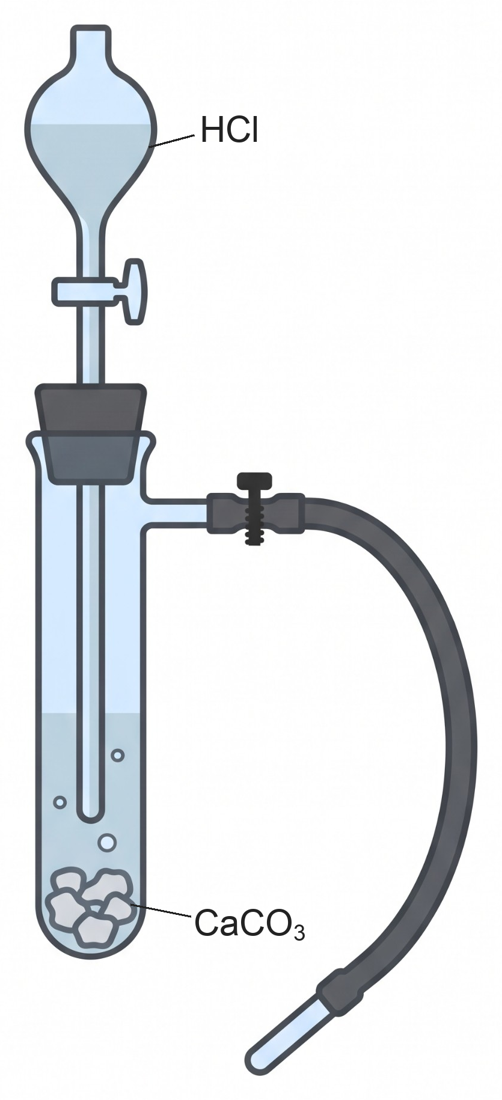
\includegraphics[width=0.86\linewidth]{rasmlar/darslik/d_co2.png}\end{center}
\noindent A)~\textsl{yig`ib bo`lmaydi}\par
\noindent B)~\textsl{suvni siqib chiqarish usulida (CO\textsubscript{2} suvda erimaydi)}\par
\noindent C)~\textsl{idishning og`zi yuqoriga, havoni siqib chiqarish usulida}\par
\noindent D)~\textsl{og`zi pastga qaratilgan idishda   ---}\par
\qsep
\end{multicols}
\medskip
\noindent\setlength{\fboxsep}{0pt}\fbox{\begin{tabular}{p{0.74\linewidth}|p{0.2\linewidth}}
\parbox[t]{0.72\linewidth}{\vspace{3pt}\textbf{Topshiriqlar (33--35) va javob variant (A--F)larini o`zaro to`g`ri moslashtiring.} Alyuminiy va rux (Al va Zn) dan iborat 11,9 g qotishma mo`l HCl eritmasida eritilganda 8,96 l (n.sh.) gaz ajraldi.
\vspace{3pt}} & \parbox[t]{0.19\linewidth}{\vspace{3pt}A~\textsl{45,38}\\[3pt]
B~\textsl{40,3}\\[3pt]
C~\textsl{90,76}\\[3pt]
D~\textsl{292}\\[3pt]
E~\textsl{146}\\[3pt]
F~\textsl{60,45}}\\ \hline
\parbox[t]{0.72\linewidth}{\vspace{2pt}\textbf{33. Qotishmadagi Al massa ulushini (\%) aniqlang.}\vspace{2pt}} & \\ \hline
\parbox[t]{0.72\linewidth}{\vspace{2pt}\textbf{34. Reaksiya uchun sarflangan 20\% li HCl massasini (g) aniqlang.}\vspace{2pt}} & \\ \hline
\parbox[t]{0.72\linewidth}{\vspace{2pt}\textbf{35. Eritmadagi tuzlarning umumiy massasini (g) aniqlang.}\vspace{2pt}} & 
\end{tabular}}
\par\bigskip
\noindent\qn{36.} P + HNO\textsubscript{3} + H\textsubscript{2}O $\to$ H\textsubscript{3}PO\textsubscript{4} + NO reaksiya tenglamasini tenglang. Oksidlovchi va qaytaruvchi oldidagi koeffitsiyentlar \textbf{yig`indisini aniqlang.}
\javob\qsep
\noindent\qn{37.} Reaksiya 30 \textdegree{}C da 72 minutda tugaydi. $\gamma$ = 2. Harorat 30 \textdegree{}C ga oshirilib, reagentlardan birining konsentratsiyasi 2 marta oshirildi (reaksiya shu modda bo`yicha 1-tartibli). Reaksiya necha minutda tugaydi?
\javob\qsep
\noindent\qn{38.} Al, Fe va Cu dan iborat aralashma mo`l NaOH eritmasi bilan ta'sirlashganda 3,36 l (n.sh.) vodorod ajraldi; xuddi shunday massadagi aralashma mo`l HCl bilan ta'sirlashganda 5,6 l (n.sh.) vodorod ajraldi, erimay qolgan qoldiq (mis) massasi 3,2 g. Aralashmaning dastlabki \textbf{massasini (g) toping.}
\javob\qsep
\noindent\qn{39.} Etanol va fenoldan iborat 18,6 g aralashma natriy bilan to`liq reaksiyaga kirishganda 3,36 l (n.sh.) vodorod ajraldi. Shu aralashmaga mo`l bromli suv ta'sir ettirilganda hosil bo`ladigan cho`kma \textbf{massasini (g) toping.}
\javob\qsep
\noindent\qn{40.} 17,8 g tristearin mo`l NaOH eritmasi bilan to`liq gidrolizlandi (sovun unumi 80\%). Hosil bo`lgan natriy stearat (M = 306 g/mol) \textbf{massasini (g) toping.}
\javob\qsep
\par\bigskip\begin{center}\textbf{\fontsize{13}{15}\selectfont YOZMA ISH}\end{center}
\noindent\qn{41.} \textbf{Topshiriqni bajarish jarayonida barcha reaksiya tenglamalarini yozing. Miqdoriy va arifmetik hisoblashlarni (unga asos bo`lgan usul yoki formulani ko`rsatgan holda) uzviy ketma-ketlikda bajaring.}\par\smallskip
Ketma-ket ulangan ikkita elektrolizyorda CuSO\textsubscript{4} va AgNO\textsubscript{3} eritmalari inert elektrodlar bilan elektroliz qilindi. Birinchi elektrolizyorning katodida 6,4 g Cu ajraldi (F = 96500 C/mol).\par
\noindent 1)\ Elektrolizyordan o`tgan zaryad miqdorini (C) hisoblang.\par
\noindent 2)\ Tok kuchi 5 A bo`lsa, elektroliz necha sekund davom etgan? O`tgan elektronlar miqdorini (mol) ham toping.\par
\noindent 3)\ Ikkinchi elektrolizyorning katodida ajralgan Ag massasini (g) aniqlang.\par
\noindent 4)\ Birinchi elektrolizyor anodida ajralgan gaz hajmini (l, n.sh.) toping. Ikkinchi elektrolizyor katodida ajralgan metallning miqdorini (mol) ham toping.\par
\noindent 5)\ Ikkala elektrolizyorda o`tgan elektronlar sonini (mol) taqqoslab, ularning teng ekanligini isbotlang. Agar tok kuchi 2 marta oshirilsa, shuncha zaryad o`tishi uchun necha sekund kerak?\par
\diqqat{Mazkur topshiriq kengaytirilgan javobni talab etib, uning yechilish usuli va shu usul asosidagi barcha hisoblash amallari javoblar varaqasida aks etishi lozim.}\qsep
\noindent\qn{42.} Quyidagi o`zgarishlar zanjirida \textit{X}, \textit{Y}, \textit{Z} noma'lum organik moddalar:\par
\[\setlength{\fboxsep}{0pt}\text{C\textsubscript{6}H\textsubscript{12}O\textsubscript{6}}\xrightarrow{\text{bijg`ish}}\text{\textit{X}}\xrightarrow{\text{H\textsubscript{2}SO\textsubscript{4} (kons.), 170 \textdegree{}C}}\text{\textit{Y}}\xrightarrow{\text{Br\textsubscript{2}}}\text{C\textsubscript{2}H\textsubscript{4}Br\textsubscript{2}}\]
\noindent 1)\ C\textsubscript{6}H\textsubscript{12}O\textsubscript{6} $\to$ \textit{X} : reaksiya tenglamasini yozing; hosil bo`lgan moddani nomlang.\par
\noindent 2)\ \textit{X} $\to$ \textit{Y} : reaksiya tenglamasini yozing; hosil bo`lgan moddani nomlang.\par
\noindent 3)\ \textit{Y} $\to$ C\textsubscript{2}H\textsubscript{4}Br\textsubscript{2} : reaksiya tenglamasini yozing; hosil bo`lgan moddani nomlang.\par
\diqqat{Mazkur topshiriq kengaytirilgan javobni talab etib, uning yechilish usuli va shu usul asosidagi barcha hisoblash amallari javoblar varaqasida aks etishi lozim.}\qsep
\noindent\qn{43.} \textbf{Topshiriqni bajarish jarayonida barcha reaksiya tenglamalarini yozing. Miqdoriy va arifmetik hisoblashlarni (unga asos bo`lgan usul yoki formulani ko`rsatgan holda) uzviy ketma-ketlikda bajaring.}\par\smallskip
Laboratoriyada 1--4-raqamli probirkalarda tartibsiz holda glyukoza, kraxmal kleysteri, tuxum oqsili va glitserin eritmalari bor. Ularni aniqlash uchun quyidagi tajribalar o`tkazildi:\par
a) 1-probirkaga yodning spirtdagi eritmasidan qo`shildi --- eritma ko`k rangga bo`yaldi.\par
b) 2-probirkaga ishqor eritmasi va bir necha tomchi mis(II)-sulfat qo`shilganda eritma qizil-binafsha rangga bo`yaldi; boshqa porsiyasiga konsentrlangan HNO\textsubscript{3} qo`shib qizdirilganda sariq rang paydo bo`ldi.\par
c) 3- va 4-probirkalarga yangi cho`ktirilgan Cu(OH)\textsubscript{2} qo`shilganda ikkalasida ham cho`kma erib, ko`k eritma hosil bo`ldi. 3-probirka qizdirilganda avval sariq, so`ng qizil cho`kma tushdi, 4-probirkada esa o`zgarish bo`lmadi.\par
\noindent 1)\ Glyukozaning Cu(OH)\textsubscript{2} bilan reaksiya tenglamasini yozing. 36 g glyukoza mo`l Cu(OH)\textsubscript{2} bilan qizdirilganda hosil bo`lgan qizil cho`kmaning massasini (g) hisoblang.\par
\noindent 2)\ 1--4-probirkalardagi moddalarni aniqlang (probirka raqami bilan moslab yozing).\par
\noindent 3)\ a), b) va c) bo`yicha kuzatilgan rang o`zgarishlarining sababini tushuntiring: qaysi funksional guruh yoki bog` bilan bog`liq?\par
\noindent 4)\ Tajribada probirkani qizdirish va konsentrlangan HNO\textsubscript{3} bilan ishlashda qanday xavfsizlik qoidalariga rioya qilish kerak? Kamida uchta qoida yozing.\par
\noindent 5)\ Glyukozaning (36 g) spirtli bijg`ishida ajraladigan CO\textsubscript{2} hajmini (l, n.sh.) hisoblang.\par
\diqqat{Mazkur topshiriq kengaytirilgan javobni talab etib, uning yechilish usuli va shu usul asosidagi barcha hisoblash amallari javoblar varaqasida aks etishi lozim.}\qsep
\newpage
\renewcommand{\curvar}{15-variant}
\thispagestyle{first}
\noindent\textit{Davriy jadvaldan foydalanish mumkin.}
\par\smallskip
\begin{multicols}{2}
\noindent\qn{1.} 29-tartib raqamli element atomida bosh kvant soni n = 2, orbital kvant soni l = 1 bo`lgan elektronlar soni nechta?

\noindent A)~\textsl{7} \hfill B)~\textsl{5} \hfill C)~\textsl{6} \hfill D)~\textsl{8}\par
\qsep
\noindent\qn{2.} Doimiy tok kuchida Ag tuzining eritmasi elektroliz qilinganda katodda ajralgan metall massasining vaqtga bog`liqligi grafikda berilgan (M(Ag) = 108 g/mol, valentlik 1).
\begin{center}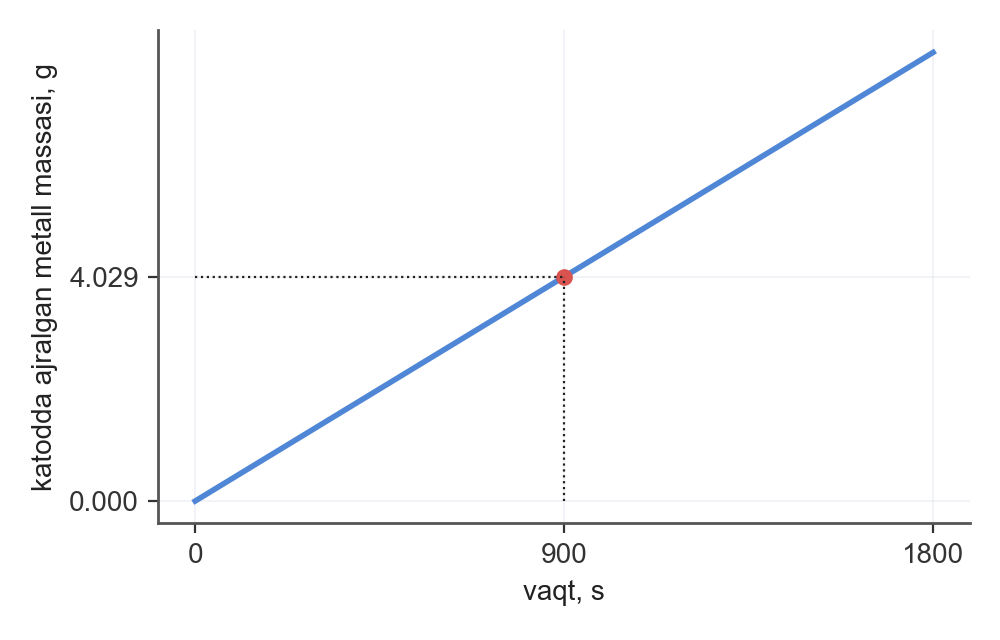
\includegraphics[width=0.86\linewidth]{rasmlar/gen/fa_v15_0.png}\end{center}
Grafikdagi nuqtaga mos kelgan jarayonda elektrodlardan o`tgan zaryad \textbf{miqdorini (C) hisoblang.}

\noindent A)~\textsl{3600} \hfill B)~\textsl{7200} \hfill C)~\textsl{1800} \hfill D)~\textsl{388800}\par
\qsep
\noindent\qn{3.} 0,1 M Ca(OH)\textsubscript{2} eritmasining normal \textbf{konsentratsiyasini (n) aniqlang.}

\noindent A)~\textsl{0,1} \hfill B)~\textsl{0,4} \hfill C)~\textsl{0,05} \hfill D)~\textsl{0,2}\par
\qsep
\noindent\qn{4.} Jadvalda bog`lar hosil qiluvchi atomlarning elektrmanfiyliklari berilgan:
\begin{center}
\renewcommand{\arraystretch}{1.15}
\fitbox{\begin{tabular}{|c|c|c|}\hline
\textbf{Bog`} & \textbf{EM (1-atom)} & \textbf{EM (2-atom)} \\ \hline
N--H & 3 & 2,1 \\ \hline
Na--Cl & 0,9 & 3 \\ \hline
H--O & 2,1 & 3,5 \\ \hline
H--Cl & 2,1 & 3 \\ \hline
\end{tabular}}
\end{center}
Qaysi bog` eng qutbli (eng ko`p ionli xarakterga ega)?

\noindent A)~\textsl{N--H} \hfill B)~\textsl{Na--Cl} \hfill C)~\textsl{H--O} \hfill D)~\textsl{H--Cl}\par
\qsep
\noindent\qn{5.} 0,2 M H\textsubscript{2}SO\textsubscript{4} eritmasining normal \textbf{konsentratsiyasini (n) aniqlang.}

\noindent A)~\textsl{0,4} \hfill B)~\textsl{0,2} \hfill C)~\textsl{0,8} \hfill D)~\textsl{0,1}\par
\qsep
\noindent\qn{6.} Zn plastinka 8 g CuSO\textsubscript{4} ni tutgan eritmaga tushirildi va Cu to`liq ajralib chiqquncha ushlab turildi. Plastinka massasi necha gramm kamayadi?

\noindent A)~\textsl{0,1} \hfill B)~\textsl{0,03} \hfill C)~\textsl{8} \hfill D)~\textsl{0,05}\par
\qsep
\noindent\qn{7.} 28 g N\textsubscript{2} 127 \textdegree{}C va 2 atm bosimda qancha hajm (l) egallaydi? (R = 0,082 l$\cdot$atm/(mol$\cdot$K))

\noindent A)~\textsl{32,8} \hfill B)~\textsl{8,2} \hfill C)~\textsl{22,4} \hfill D)~\textsl{16,4}\par
\qsep
\noindent\qn{8.} 2 mol Ba(OH)\textsubscript{2} va 2 mol HNO\textsubscript{3} suvda eritilib, eritma hajmi 4 l ga yetkazildi. Eritmadagi barcha ionlarning umumiy molyar \textbf{konsentratsiyasini (mol/l) aniqlang} (kuchli elektrolitlar to`liq dissotsilanadi).

\noindent A)~\textsl{1} \hfill B)~\textsl{5} \hfill C)~\textsl{2,5} \hfill D)~\textsl{1,25}\par
\qsep
\noindent\qn{9.} Rasmda molekulaning elektron (Lyuis) formulasi berilgan.
\begin{center}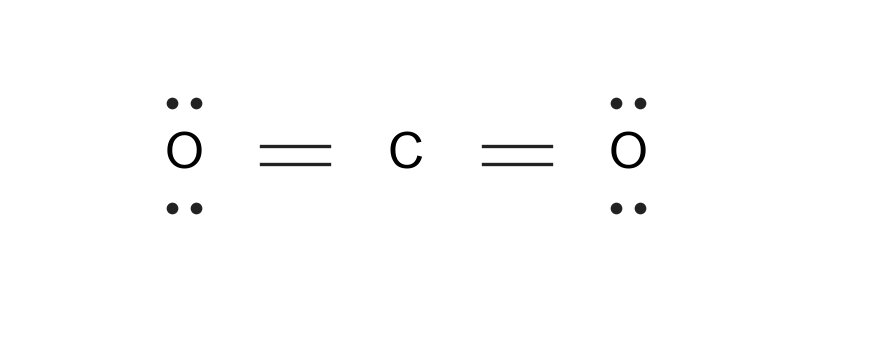
\includegraphics[width=0.86\linewidth]{rasmlar/gen/lw_864378.png}\end{center}
Molekulaning \textbf{formulasini aniqlang.}

\noindent A)~\textsl{Cl\textsubscript{2}} \hfill B)~\textsl{H\textsubscript{2}O} \hfill C)~\textsl{CO\textsubscript{2}} \hfill D)~\textsl{HCl}\par
\qsep
\noindent\qn{10.} Tabiiy elementning ikki izotopi: \textsuperscript{79}Br (50\%) va \textsuperscript{81}Br (50\%). Elementning o`rtacha nisbiy atom \textbf{massasini aniqlang.}

\noindent A)~\textsl{79} \hfill B)~\textsl{80} \hfill C)~\textsl{81} \hfill D)~\textsl{160}\par
\qsep
\noindent\qn{11.} Laboratoriyada Na\textsubscript{2}SO\textsubscript{4} eritmalari quyidagicha tayyorlangan:
\begin{center}
\renewcommand{\arraystretch}{1.15}
\fitbox{\begin{tabular}{|c|c|c|}\hline
\textbf{Idish} & \textbf{Eritma massasi, g} & \textbf{$\omega$(Na\textsubscript{2}SO\textsubscript{4}), \%} \\ \hline
A & 50 & 12 \\ \hline
B & 300 & 40 \\ \hline
\end{tabular}}
\end{center}
Bu ikki eritma bir idishga quyilib va ustiga 50 g suv qo`shilsa, yangi eritmadagi Na\textsubscript{2}SO\textsubscript{4} ning massa ulushi (\%) qancha bo`ladi?

\noindent A)~\textsl{26} \hfill B)~\textsl{52} \hfill C)~\textsl{31,5} \hfill D)~\textsl{16}\par
\qsep
\noindent\qn{12.} Jadvalda NaCl ning ikki eritmasi haqida ma'lumot berilgan:
\begin{center}
\renewcommand{\arraystretch}{1.15}
\fitbox{\begin{tabular}{|c|c|c|}\hline
\textbf{Eritma} & \textbf{Massasi, g} & \textbf{Massa ulushi, \%} \\ \hline
1 & 50 & 5 \\ \hline
2 & 300 & 30 \\ \hline
\end{tabular}}
\end{center}
Eritmalar aralashtirildi. Hosil bo`lgan eritmaning massa \textbf{ulushini (\%) aniqlang.}

\noindent A)~\textsl{17,5} \hfill B)~\textsl{26,43} \hfill C)~\textsl{35} \hfill D)~\textsl{8,57}\par
\qsep
\noindent\qn{13.} Faqat oksidlovchi bo`la oladigan \textbf{ionlarni aniqlang}: 1) Fe\textsuperscript{3+}; 2) S\textsuperscript{2$-$}; 3) Cl\textsuperscript{$-$}; 4) Zn\textsuperscript{2+}

\noindent A)~\textsl{3} \hfill B)~\textsl{4} \hfill C)~\textsl{3, 4} \hfill D)~\textsl{2}\par
\qsep
\noindent\qn{14.} D-metallar va ularning birikmalari haqida qaysi fikrlar to`g`ri? 1) Fe(OH)\textsubscript{2} havoda qo`ng`ir rangga o`tadi; 2) Xrom (VI) oksidi (CrO\textsubscript{3}) kislotali oksid; 3) Cu(OH)\textsubscript{2} qizdirilganda CuO ga parchalanadi; 4) Temir sovuq konsentrlangan HNO\textsubscript{3} da passivlanadi

\noindent\begin{tabular}{@{}p{0.47\linewidth}@{}p{0.47\linewidth}@{}}
A)~\textsl{2, 3, 4} & B)~\textsl{1, 2, 4} \\
C)~\textsl{1, 3, 4} & D)~\textsl{1, 2, 3, 4} \\
\end{tabular}\par
\qsep
\noindent\qn{15.} Reaksiya tenglamasi: Mg(HCO\textsubscript{3})\textsubscript{2} $\to$ MgCO\textsubscript{3} + CO\textsubscript{2} + H\textsubscript{2}O. Reaksiyaga tarkibida 20\% aralashma bo`lgan 36,5 g namuna (asosiy modda Mg(HCO\textsubscript{3})\textsubscript{2}) kirishdi. CO\textsubscript{2} \textbf{massasini (g) hisoblang.}

\noindent A)~\textsl{17,6} \hfill B)~\textsl{4,4} \hfill C)~\textsl{13,2} \hfill D)~\textsl{8,8}\par
\qsep
\noindent\qn{16.} SO\textsubscript{3} + 2KOH $\to$ K\textsubscript{2}SO\textsubscript{4} + H\textsubscript{2}O jarayoni uchun 80 g SO\textsubscript{3} olingan. KOH \textbf{massasini (g) aniqlang.}

\noindent A)~\textsl{28} \hfill B)~\textsl{224} \hfill C)~\textsl{112} \hfill D)~\textsl{56}\par
\qsep
\noindent\qn{17.} BaCl\textsubscript{2} + Na\textsubscript{2}SO\textsubscript{4} $\to$ BaSO\textsubscript{4} + 2NaCl reaksiyasida tarkibida 20\% aralashma bo`lgan 260 g namuna (asosiy modda BaCl\textsubscript{2}) ishtirok etdi. BaSO\textsubscript{4} \textbf{massasini (g) toping.}

\noindent A)~\textsl{233} \hfill B)~\textsl{466} \hfill C)~\textsl{116,5} \hfill D)~\textsl{349,5}\par
\qsep
\noindent\qn{18.} Quyidagi mineral o`g`itlardan qaysilari fosforli o`g`itlar jumlasiga kiradi? 1) Ca(H\textsubscript{2}PO\textsubscript{4})\textsubscript{2}; 2) Ca\textsubscript{3}(PO\textsubscript{4})\textsubscript{2}; 3) K\textsubscript{2}SO\textsubscript{4}; 4) (NH\textsubscript{4})\textsubscript{2}HPO\textsubscript{4}

\noindent A)~\textsl{3, 4} \hfill B)~\textsl{1, 2} \hfill C)~\textsl{1, 4} \hfill D)~\textsl{2, 3}\par
\qsep
\noindent\qn{19.} Reaksiya tenglamasi: 2NaNO\textsubscript{3} $\to$ 2NaNO\textsubscript{2} + O\textsubscript{2}. Reaksiyaga 17 g NaNO\textsubscript{3} kirishdi. NaNO\textsubscript{2} \textbf{massasini (g) hisoblang.}

\noindent A)~\textsl{27,6} \hfill B)~\textsl{6,9} \hfill C)~\textsl{20,7} \hfill D)~\textsl{13,8}\par
\qsep
\noindent\qn{20.} 15 g C\textsubscript{2}H\textsubscript{6} dan quyidagi ikki bosqichda C\textsubscript{2}H\textsubscript{5}OH olinadi: 1) C\textsubscript{2}H\textsubscript{6} + Cl\textsubscript{2} $\to$ C\textsubscript{2}H\textsubscript{5}Cl + HCl (unum 60\%); 2) C\textsubscript{2}H\textsubscript{5}Cl + KOH $\to$ C\textsubscript{2}H\textsubscript{5}OH + KCl (unum 75\%). Oxirgi mahsulot C\textsubscript{2}H\textsubscript{5}OH ning \textbf{massasini (g) toping.}

\noindent A)~\textsl{10,35} \hfill B)~\textsl{17,25} \hfill C)~\textsl{13,8} \hfill D)~\textsl{23}\par
\qsep
\noindent\qn{21.} Alken, alkadiyen va alkinlar haqida qaysi fikrlar to`g`ri? 1) Propenga HBr birikishi Markovnikov qoidasiga bo`ysunadi; 2) Alkinlar uchun umumiy formula CnH\textsubscript{2}n+2; 3) Alkenlar KMnO\textsubscript{4} ning suvli eritmasi bilan glikol hosil qiladi; 4) Asetilenni Kucherov reaksiyasi bilan sirka aldegidiga aylantirish mumkin

\noindent A)~\textsl{1, 3, 4} \hfill B)~\textsl{1, 2} \hfill C)~\textsl{2, 3, 4} \hfill D)~\textsl{3, 4}\par
\qsep
\noindent\qn{22.} Arenlar, neft va tabiiy gaz haqida qaysi fikrlar to`g`ri? 1) Naftalin -- bir halqali aren; 2) Benzol uchun birikish reaksiyalari mutlaqo xos emas; 3) Benzolda 6 ta sp\textsuperscript{2} gibridlangan uglerod bor; 4) Tabiiy gazning asosiy qismi propan

\noindent A)~\textsl{2, 3} \hfill B)~\textsl{3} \hfill C)~\textsl{1, 4} \hfill D)~\textsl{3, 4}\par
\qsep
\noindent\qn{23.} Reaksiya tenglamasi: C\textsubscript{6}H\textsubscript{5}OH + NaOH $\to$ C\textsubscript{6}H\textsubscript{5}ONa + H\textsubscript{2}O. Reaksiyaga tarkibida 75\% aralashma bo`lgan 32 g namuna (asosiy modda NaOH) kirishdi. C\textsubscript{6}H\textsubscript{5}OH \textbf{massasini (g) hisoblang.}

\noindent A)~\textsl{18,8} \hfill B)~\textsl{37,6} \hfill C)~\textsl{9,4} \hfill D)~\textsl{28,2}\par
\qsep
\noindent\qn{24.} Aldegid va ketonlar haqida qaysi fikrlar to`g`ri? 1) Aseton Cu(OH)\textsubscript{2} ni qaytaradi; 2) Formalin --- formaldegidning 40\% li eritmasi; 3) Formaldegid gaz holatda, suvda yaxshi eriydi; 4) Sirka aldegid Kucherov reaksiyasi bilan olinadi

\noindent A)~\textsl{2, 4} \hfill B)~\textsl{2, 3} \hfill C)~\textsl{2, 3, 4} \hfill D)~\textsl{1, 3}\par
\qsep
\noindent\qn{25.} C\textsubscript{4}H\textsubscript{10} alkanning izomerlari soni nechta?

\noindent A)~\textsl{2} \hfill B)~\textsl{3} \hfill C)~\textsl{1} \hfill D)~\textsl{4}\par
\qsep
\noindent\qn{26.} 442 g triolein (M = 884) nikel katalizatori ishtirokida to`liq gidrogenlandi. Sarflangan vodorod \textbf{hajmini (l, n.sh.) aniqlang.}

\noindent A)~\textsl{11,2} \hfill B)~\textsl{67,2} \hfill C)~\textsl{33,6} \hfill D)~\textsl{16,8}\par
\qsep
\noindent\qn{27.} Uglevodlar haqida qaysi fikrlar to`g`ri? 1) Maltoza gidrolizlanganda ikki molekula glyukoza hosil qiladi; 2) Kraxmal yod bilan ko`k rang beradi; 3) Selluloza $\beta$-glyukoza qoldiqlaridan iborat; 4) Fruktoza ketospirt

\noindent\begin{tabular}{@{}p{0.47\linewidth}@{}p{0.47\linewidth}@{}}
A)~\textsl{2, 3, 4} & B)~\textsl{1, 2, 3, 4} \\
C)~\textsl{1, 3, 4} & D)~\textsl{1, 2, 4} \\
\end{tabular}\par
\qsep
\noindent\qn{28.} Aminlar, aminokislotalar va oqsillar haqida qaysi fikrlar to`g`ri? 1) Dipeptidda 2 ta peptid bog` bor; 2) Anilin bromli suv bilan oq cho`kma beradi; 3) Oqsillar biuret reaksiyasini beradi; 4) Glitsin optik faol

\noindent A)~\textsl{4} \hfill B)~\textsl{1} \hfill C)~\textsl{2, 3} \hfill D)~\textsl{1, 2}\par
\qsep
\noindent\qn{29.} Reaksiya tenglamasi: C\textsubscript{2}H\textsubscript{4} + Cl\textsubscript{2} $\to$ C\textsubscript{2}H\textsubscript{4}Cl\textsubscript{2}. Reaksiyaga 7 g C\textsubscript{2}H\textsubscript{4} kirishdi. C\textsubscript{2}H\textsubscript{4}Cl\textsubscript{2} \textbf{massasini (g) hisoblang.}

\noindent A)~\textsl{49,5} \hfill B)~\textsl{24,75} \hfill C)~\textsl{12,38} \hfill D)~\textsl{37,12}\par
\qsep
\noindent\qn{30.} Rasmda ammiak olish tajribasi ko`rsatilgan. Qaysi moddalar aralashmasi qizdirilmoqda?
\begin{center}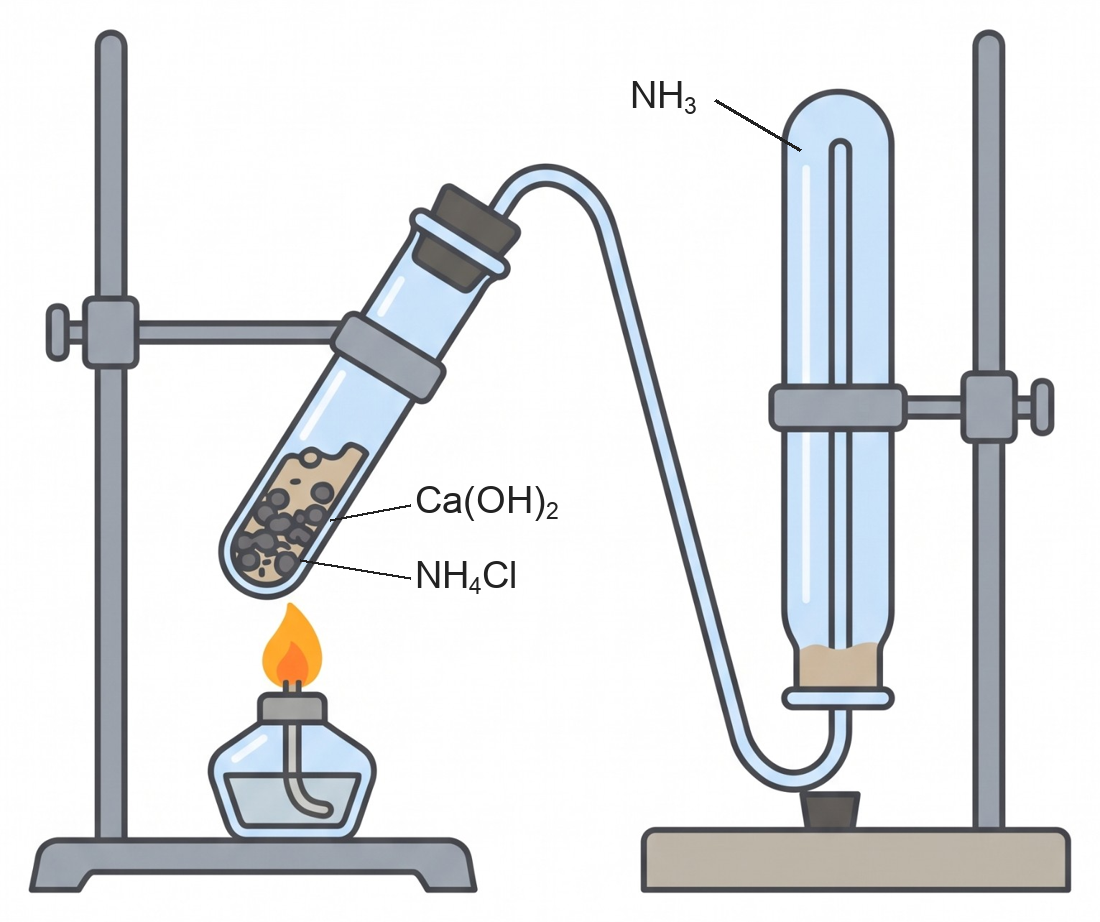
\includegraphics[width=0.86\linewidth]{rasmlar/darslik/d_nh3_lab.png}\end{center}

\noindent\begin{tabular}{@{}p{0.47\linewidth}@{}p{0.47\linewidth}@{}}
A)~\textsl{NH\textsubscript{4}Cl va Ca(OH)\textsubscript{2}} & B)~\textsl{NaCl va H\textsubscript{2}SO\textsubscript{4}} \\
C)~\textsl{Zn va HCl} & D)~\textsl{CaCO\textsubscript{3} va HCl} \\
\end{tabular}\par
\qsep
\noindent\qn{31.} 200 g 5\% li eritma tayyorlash uchun 50\% li eritmadan necha gramm olish kerak (qolgani suv)?

\noindent A)~\textsl{180} \hfill B)~\textsl{10} \hfill C)~\textsl{40} \hfill D)~\textsl{20}\par
\qsep
\noindent\qn{32.} Kimyoviy laboratoriyada pipetka nima uchun ishlatiladi?
\noindent A)~\textsl{qattiq moddalarni yuqori haroratda qizdirish}\par
\noindent B)~\textsl{titrlashda reagent hajmini aniq o`lchash}\par
\noindent C)~\textsl{vakuum ostida filtrlash}\par
\noindent D)~\textsl{eritmaning kichik hajmlarini o`lchab olish   ---}\par
\qsep
\end{multicols}
\medskip
\noindent\setlength{\fboxsep}{0pt}\fbox{\begin{tabular}{p{0.74\linewidth}|p{0.2\linewidth}}
\parbox[t]{0.72\linewidth}{\vspace{3pt}\textbf{Topshiriqlar (33--35) va javob variant (A--F)larini o`zaro to`g`ri moslashtiring.} Sirka kislota va etanoldan iborat 25,8 g aralashmaga mo`l NaHCO\textsubscript{3} eritmasi qo`shilganda 4,48 l (n.sh.) gaz ajraldi. Xuddi shunday massadagi aralashma natriy bilan ta'sirlashganda esa 5,6 l (n.sh.) vodorod ajraldi.
\vspace{3pt}} & \parbox[t]{0.19\linewidth}{\vspace{3pt}A~\textsl{6}\\[3pt]
B~\textsl{9,6}\\[3pt]
C~\textsl{12}\\[3pt]
D~\textsl{11,04}\\[3pt]
E~\textsl{13,12}\\[3pt]
F~\textsl{13,8}}\\ \hline
\parbox[t]{0.72\linewidth}{\vspace{2pt}\textbf{33. Aralashmadagi sirka kislota massasini (g) aniqlang.}\vspace{2pt}} & \\ \hline
\parbox[t]{0.72\linewidth}{\vspace{2pt}\textbf{34. Aralashmadagi etanol massasini (g) aniqlang.}\vspace{2pt}} & \\ \hline
\parbox[t]{0.72\linewidth}{\vspace{2pt}\textbf{35. Aralashma to`liq neytrallanganda (faqat kislota) hosil bo`lgan natriy atsetat massasini (g) aniqlang (reaksiya unumi 80\%).}\vspace{2pt}} & 
\end{tabular}}
\par\bigskip
\noindent\qn{36.} K\textsubscript{2}Cr\textsubscript{2}O\textsubscript{7} + KI + H\textsubscript{2}SO\textsubscript{4} $\to$ Cr\textsubscript{2}(SO\textsubscript{4})\textsubscript{3} + I\textsubscript{2} + K\textsubscript{2}SO\textsubscript{4} + H\textsubscript{2}O reaksiya tenglamasini tenglang. Oksidlovchi va qaytaruvchi oldidagi koeffitsiyentlar \textbf{yig`indisini aniqlang.}
\javob\qsep
\noindent\qn{37.} 14 g Fe reaksiyaga kirishdi (Fe + 2HCl $\to$ FeCl\textsubscript{2} + H\textsubscript{2}). Ajralgan H\textsubscript{2} \textbf{hajmini (l, n.sh.) hisoblang} (unum 90\%).
\javob\qsep
\noindent\qn{38.} 75,2 g Cu(NO\textsubscript{3})\textsubscript{2} qizdirilganda qisman parchalandi, qattiq qoldiq massasi 53,6 g bo`ldi. Ajralgan gazlar (n.sh.) \textbf{hajmini (l) hisoblang.}
\javob\qsep
\noindent\qn{39.} Etilen va asetilendan iborat 3,36 l (n.sh.) aralashma bromli suvdan o`tkazilganda 40 g brom yutildi. Aralashmadagi asetilenning \textbf{hajmini (l, n.sh.) toping.}
\javob\qsep
\noindent\qn{40.} 18 g sirka kislota va 6,4 g metanol dan 80\% unum bilan murakkab efir olindi. Efir \textbf{massasini (g) toping.}
\javob\qsep
\par\bigskip\begin{center}\textbf{\fontsize{13}{15}\selectfont YOZMA ISH}\end{center}
\noindent\qn{41.} \textbf{Topshiriqni bajarish jarayonida barcha reaksiya tenglamalarini yozing. Miqdoriy va arifmetik hisoblashlarni (unga asos bo`lgan usul yoki formulani ko`rsatgan holda) uzviy ketma-ketlikda bajaring.}\par\smallskip
Hajmi 1 l bo`lgan idishga 0,4 mol SO\textsubscript{2} va ma'lum miqdorda O\textsubscript{2} solindi hamda katalizator ishtirokida qizdirildi: 2SO\textsubscript{2} + O\textsubscript{2} $\rightleftarrows$ 2SO\textsubscript{3}. Muvozanat qaror topganda idishda SO\textsubscript{2}, O\textsubscript{2} va SO\textsubscript{3} ning mol nisbati 1 : 1 : 3 bo`ldi.\par
Hosil bo`lgan SO\textsubscript{3} ning hammasi 100 g 30\% li H\textsubscript{2}SO\textsubscript{4} eritmasiga yuttirildi (oleum hosil bo`lmadi, SO\textsubscript{3} to`liq suv bilan reaksiyaga kirishdi). Olingan eritmaga mo`l BaCl\textsubscript{2} eritmasi qo`shildi.\par
\noindent 1)\ O\textsubscript{2} ning boshlang`ich miqdorini (mol) va muvozanat konstantasini (K) hisoblang.\par
\noindent 2)\ SO\textsubscript{2} ning necha foizi reaksiyaga kirishgan? Muvozanatda SO\textsubscript{3} ning hajmiy ulushini (\%) ham toping.\par
\noindent 3)\ SO\textsubscript{3} yuttirilgandan keyingi eritmada H\textsubscript{2}SO\textsubscript{4} ning massa ulushini (\%) aniqlang.\par
\noindent 4)\ BaCl\textsubscript{2} qo`shilganda hosil bo`lgan cho`kma massasini (g) toping. BaCl\textsubscript{2} sarfini (g) ham toping.\par
\noindent 5)\ Doimiy haroratda idish hajmi 2 marta kamaytirilsa (v = k$\cdot$[SO\textsubscript{2}]\textsuperscript{2}$\cdot$[O\textsubscript{2}]), to`g`ri reaksiya tezligi necha marta o`zgaradi? Shuningdek muvozanatda umumiy bosimning boshlang`ich bosimga nisbatini (T = const) toping.\par
\diqqat{Mazkur topshiriq kengaytirilgan javobni talab etib, uning yechilish usuli va shu usul asosidagi barcha hisoblash amallari javoblar varaqasida aks etishi lozim.}\qsep
\noindent\qn{42.} Quyidagi o`zgarishlar zanjirida \textit{X}, \textit{Y}, \textit{Z} noma'lum organik moddalar:\par
\[\setlength{\fboxsep}{0pt}\text{C\textsubscript{2}H\textsubscript{5}Cl}\xrightarrow{\text{KOH (spirtli)}}\text{\textit{X}}\xrightarrow{\text{Br\textsubscript{2}}}\text{\textit{Y}}\xrightarrow{\text{KOH (spirtli)}}\text{\textit{Z}}\xrightarrow{\text{C (aktiv), 600 \textdegree{}C}}\text{C\textsubscript{6}H\textsubscript{6}}\]
\noindent 1)\ C\textsubscript{2}H\textsubscript{5}Cl $\to$ \textit{X} : reaksiya tenglamasini yozing; hosil bo`lgan moddani nomlang.\par
\noindent 2)\ \textit{X} $\to$ \textit{Y} : reaksiya tenglamasini yozing; hosil bo`lgan moddani nomlang.\par
\noindent 3)\ \textit{Y} $\to$ \textit{Z} : reaksiya tenglamasini yozing; hosil bo`lgan moddani nomlang.\par
\noindent 4)\ \textit{Z} $\to$ C\textsubscript{6}H\textsubscript{6} : reaksiya tenglamasini yozing; hosil bo`lgan moddani nomlang.\par
\diqqat{Mazkur topshiriq kengaytirilgan javobni talab etib, uning yechilish usuli va shu usul asosidagi barcha hisoblash amallari javoblar varaqasida aks etishi lozim.}\qsep
\noindent\qn{43.} \textbf{Topshiriqni bajarish jarayonida barcha reaksiya tenglamalarini yozing. Miqdoriy va arifmetik hisoblashlarni (unga asos bo`lgan usul yoki formulani ko`rsatgan holda) uzviy ketma-ketlikda bajaring.}\par\smallskip
67,2 l (n.sh.) ammiak katalizator ishtirokida kislorodda oksidlandi (4NH\textsubscript{3} + 5O\textsubscript{2} $\to$ 4NO + 6H\textsubscript{2}O, unum 80\%). Hosil bo`lgan NO ni nitrat kislotagacha qayta ishlash unumi 80\%.\par
\noindent 1)\ Hosil bo`lgan NO hajmini (l, n.sh.) hisoblang. Hosil bo`lgan NO ning massasini (g) ham toping.\par
\noindent 2)\ Nitrat kislota ishlab chiqarishning keyingi bosqichlari tenglamalarini yozing va olingan HNO\textsubscript{3} massasini (g) toping.\par
\noindent 3)\ Hosil bo`lgan HNO\textsubscript{3} ni to`liq neytrallash uchun zarur ammiak hajmini (l, n.sh.) aniqlang (NH\textsubscript{3} + HNO\textsubscript{3} $\to$ NH\textsubscript{4}NO\textsubscript{3}).\par
\noindent 4)\ Hosil bo`lgan ammoniy nitrat massasini (g) hisoblang va azotning massa ulushini (\%) toping.\par
\noindent 5)\ Olingan HNO\textsubscript{3} dan 63\% li eritma necha gramm tayyorlanadi?\par
\diqqat{Mazkur topshiriq kengaytirilgan javobni talab etib, uning yechilish usuli va shu usul asosidagi barcha hisoblash amallari javoblar varaqasida aks etishi lozim.}\qsep
\newpage
\renewcommand{\curvar}{16-variant}
\thispagestyle{first}
\noindent\textit{Davriy jadvaldan foydalanish mumkin.}
\par\smallskip
\begin{multicols}{2}
\noindent\qn{1.} 2SO\textsubscript{2} + O\textsubscript{2} $\rightleftarrows$ 2SO\textsubscript{3} reaksiyasi 4 l hajmli idishda o`tkazildi. Ma'lumotlar jadvalda berilgan:
\begin{center}
\renewcommand{\arraystretch}{1.15}
\fitbox{\begin{tabular}{|c|c|c|c|}\hline
\textbf{Modda} & \textbf{SO\textsubscript{2}} & \textbf{O\textsubscript{2}} & \textbf{SO\textsubscript{3}} \\ \hline
Boshlang`ich, mol & 6 & 4 & 0 \\ \hline
Muvozanatda, mol & --- & --- & 4 \\ \hline
\end{tabular}}
\end{center}
SO\textsubscript{2} ning necha foizi reaksiyaga \textbf{kirishganini aniqlang.}

\noindent A)~\textsl{33,3} \hfill B)~\textsl{66,7} \hfill C)~\textsl{100} \hfill D)~\textsl{133,3}\par
\qsep
\noindent\qn{2.} 16,4 l CO\textsubscript{2} -23 \textdegree{}C va 0,5 atm bosimda necha gramm keladi? (R = 0,082 l$\cdot$atm/(mol$\cdot$K))

\noindent A)~\textsl{35,2} \hfill B)~\textsl{8,8} \hfill C)~\textsl{17,6} \hfill D)~\textsl{32,21}\par
\qsep
\noindent\qn{3.} Quyidagi moddalarning qaysilarida donor--akseptor bog` mavjud? 1) CO\textsubscript{2}; 2) KNO\textsubscript{3}; 3) NaOH; 4) (NH\textsubscript{4})\textsubscript{2}SO\textsubscript{4}

\noindent A)~\textsl{3, 4} \hfill B)~\textsl{2, 4} \hfill C)~\textsl{2, 3} \hfill D)~\textsl{4}\par
\qsep
\noindent\qn{4.} N\textsubscript{2}O\textsubscript{5} moddaning parchalanish reaksiyasida konsentratsiyaning vaqt bo`yicha o`zgarishi jadvalda berilgan:
\begin{center}
\renewcommand{\arraystretch}{1.15}
\fitbox{\begin{tabular}{|c|c|}\hline
\textbf{t, min} & \textbf{c, mol/l} \\ \hline
0 & 2 \\ \hline
2 & 1,7 \\ \hline
4 & 1,4 \\ \hline
6 & 1,1 \\ \hline
\end{tabular}}
\end{center}
0-minutdan 2-minutgacha o`rtacha tezlikni mol/(l$\cdot$min) \textbf{hisoblang.}

\noindent A)~\textsl{0,3} \hfill B)~\textsl{0,075} \hfill C)~\textsl{1} \hfill D)~\textsl{0,15}\par
\qsep
\noindent\qn{5.} Faqat qaytaruvchi bo`la oladigan \textbf{ionlarni aniqlang}: 1) Cl\textsuperscript{$-$}; 2) Fe\textsuperscript{3+}; 3) Fe\textsuperscript{2+}; 4) K\textsuperscript{+}

\noindent A)~\textsl{2, 3} \hfill B)~\textsl{3, 4} \hfill C)~\textsl{1, 4} \hfill D)~\textsl{1}\par
\qsep
\noindent\qn{6.} 0,5 mol CO\textsubscript{2} tarkibidagi atomlar \textbf{sonini toping} (N\textsubscript{A} = 6,02$\cdot$10\textsuperscript{23}). Javobni 10\textsuperscript{23} birligida yozing.

\noindent A)~\textsl{1,806} \hfill B)~\textsl{0,451} \hfill C)~\textsl{0,903} \hfill D)~\textsl{0,301}\par
\qsep
\noindent\qn{7.} Hajmi 2 l bo`lgan idishda A modda miqdori 30 s davomida 6 mol ga kamaydi. Reaksiyaning o`rtacha tezligini (mol/(l$\cdot$s)) \textbf{toping.}

\noindent A)~\textsl{0,1} \hfill B)~\textsl{0,2} \hfill C)~\textsl{3} \hfill D)~\textsl{0,4}\par
\qsep
\noindent\qn{8.} 0,1 M H\textsubscript{3}PO\textsubscript{4} eritmasining normal \textbf{konsentratsiyasini (n) aniqlang.}

\noindent A)~\textsl{0,1} \hfill B)~\textsl{0,6} \hfill C)~\textsl{0,3} \hfill D)~\textsl{0,033}\par
\qsep
\noindent\qn{9.} Zn + HNO\textsubscript{3} $\to$ Zn(NO\textsubscript{3})\textsubscript{2} + NO + H\textsubscript{2}O reaksiyasida 6 mol Zn erisa, HNO\textsubscript{3} ning necha moli oksidlovchi vazifasini bajaradi?

\noindent A)~\textsl{16} \hfill B)~\textsl{12} \hfill C)~\textsl{8} \hfill D)~\textsl{4}\par
\qsep
\noindent\qn{10.} 2SO\textsubscript{2} + O\textsubscript{2} $\rightleftarrows$ 2SO\textsubscript{3} reaksiyada muvozanat holatida [SO\textsubscript{2}] = 0,5, [O\textsubscript{2}] = 0,5, [SO\textsubscript{3}] = 4 mol/l. Muvozanat \textbf{konstantasini (K) hisoblang.}

\noindent A)~\textsl{256} \hfill B)~\textsl{128} \hfill C)~\textsl{64} \hfill D)~\textsl{16}\par
\qsep
\noindent\qn{11.} Quyidagi tuzlarning qaysilari suvli eritmasi ishqoriy muhitga ega? 1) NaNO\textsubscript{2}; 2) CuSO\textsubscript{4}; 3) NH\textsubscript{4}Cl; 4) NaCl

\noindent A)~\textsl{1} \hfill B)~\textsl{1, 2} \hfill C)~\textsl{3} \hfill D)~\textsl{4}\par
\qsep
\noindent\qn{12.} Na\textsubscript{2}CO\textsubscript{3}$\cdot$10H\textsubscript{2}O kristallogidrat namunasi (50 g) bosqichma-bosqich qizdirilganda uning massasi o`zgarishi grafikda keltirilgan.
\begin{center}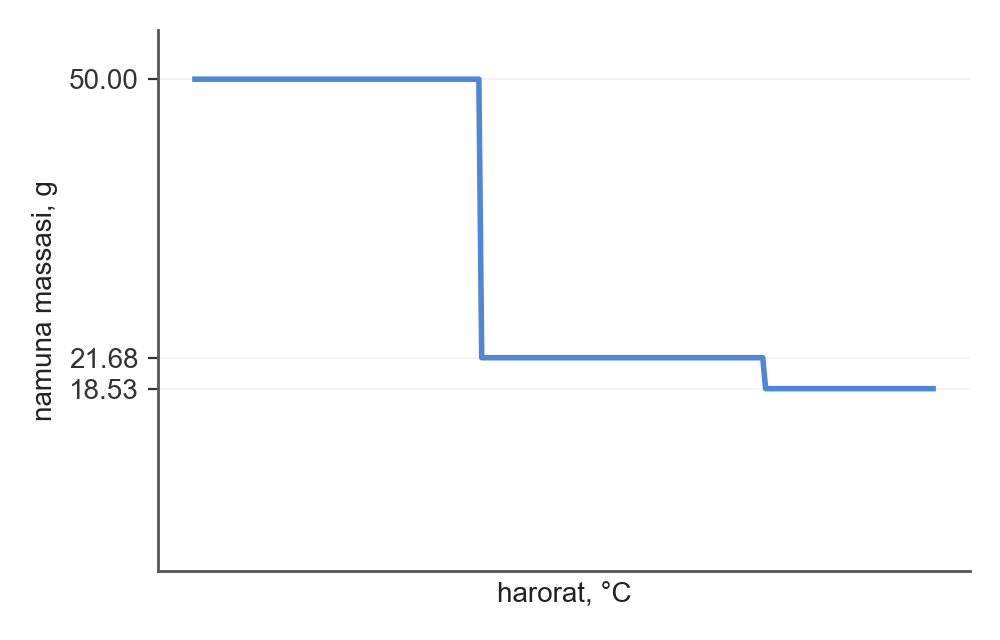
\includegraphics[width=0.86\linewidth]{rasmlar/gen/hy_v16_0.png}\end{center}
To`liq suvsizlangandan keyin qolgan Na\textsubscript{2}CO\textsubscript{3} ning \textbf{massasini (g) toping.}

\noindent A)~\textsl{31,47} \hfill B)~\textsl{21,68} \hfill C)~\textsl{18,53} \hfill D)~\textsl{37,06}\par
\qsep
\noindent\qn{13.} NaCl ning suvli eritmasi inert elektrodlar bilan elektroliz qilinganda qaysi moddalar ajraladi?

\noindent\begin{tabular}{@{}p{0.47\linewidth}@{}p{0.47\linewidth}@{}}
A)~\textsl{Zn, H\textsubscript{2} va O\textsubscript{2}} & B)~\textsl{Ag va O\textsubscript{2}} \\
C)~\textsl{Cu va O\textsubscript{2}} & D)~\textsl{H\textsubscript{2}, Cl\textsubscript{2} va NaOH} \\
\end{tabular}\par
\qsep
\noindent\qn{14.} Rasmdagi o`zgarishlar zanjirida \textit{X} moddaning \textbf{formulasini aniqlang.}
\begin{center}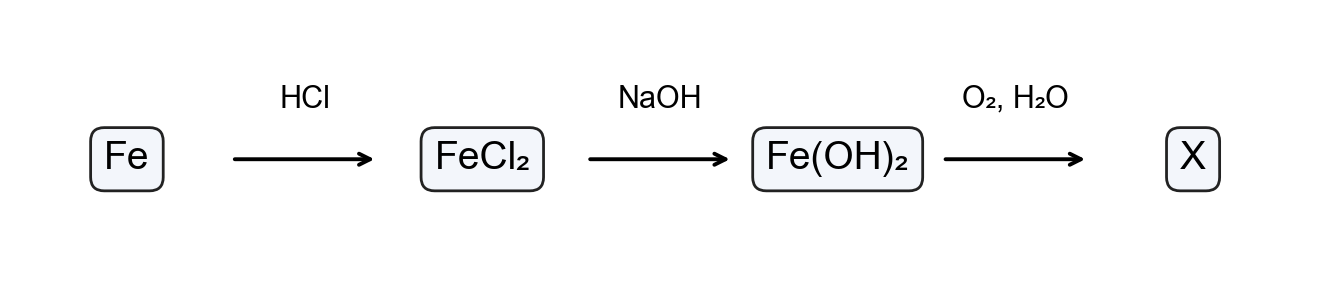
\includegraphics[width=0.86\linewidth]{rasmlar/gen/ci_509279.png}\end{center}

\noindent A)~\textsl{Fe(OH)\textsubscript{3}} \hfill B)~\textsl{FeCl\textsubscript{2}} \hfill C)~\textsl{SO\textsubscript{3}} \hfill D)~\textsl{Fe(OH)\textsubscript{2}}\par
\qsep
\noindent\qn{15.} Cu $\to$ ? $\to$ ? $\to$ ? o`zgarishlar zanjirida (reagentlar: O\textsubscript{2}, H\textsubscript{2}SO\textsubscript{4}, NaOH) 1-bosqichda hosil bo`ladigan modda \textbf{formulasini toping.}

\noindent A)~\textsl{Na\textsubscript{2}SO\textsubscript{3}} \hfill B)~\textsl{Ca(OH)\textsubscript{2}} \hfill C)~\textsl{CuO} \hfill D)~\textsl{NaCl}\par
\qsep
\noindent\qn{16.} NH\textsubscript{3} + H\textsubscript{3}PO\textsubscript{4} $\to$ NH\textsubscript{4}H\textsubscript{2}PO\textsubscript{4} jarayoni uchun 4,48 l (n.sh.) NH\textsubscript{3} olingan (unum 90\%). NH\textsubscript{4}H\textsubscript{2}PO\textsubscript{4} \textbf{miqdorini (mol) aniqlang.}

\noindent A)~\textsl{0,2} \hfill B)~\textsl{0,36} \hfill C)~\textsl{0,18} \hfill D)~\textsl{0,09}\par
\qsep
\noindent\qn{17.} 14,8 g Mg(NO\textsubscript{3})\textsubscript{2} to`liq parchalanguncha qizdirildi. Qattiq qoldiq \textbf{massasini (g) aniqlang.}

\noindent A)~\textsl{4} \hfill B)~\textsl{14,8} \hfill C)~\textsl{8} \hfill D)~\textsl{2}\par
\qsep
\noindent\qn{18.} S + O\textsubscript{2} $\to$ SO\textsubscript{2} jarayoni uchun 8,96 l (n.sh.) O\textsubscript{2} olingan. SO\textsubscript{2} \textbf{hajmini (l, n.sh.) aniqlang.}

\noindent A)~\textsl{17,92} \hfill B)~\textsl{4,48} \hfill C)~\textsl{8,96} \hfill D)~\textsl{13,44}\par
\qsep
\noindent\qn{19.} 2NO + O\textsubscript{2} $\to$ 2NO\textsubscript{2} jarayoni uchun 8,96 l (n.sh.) O\textsubscript{2} olingan. NO \textbf{hajmini (l, n.sh.) aniqlang.}

\noindent A)~\textsl{4,48} \hfill B)~\textsl{17,92} \hfill C)~\textsl{35,84} \hfill D)~\textsl{8,96}\par
\qsep
\noindent\qn{20.} C\textsubscript{3}H\textsubscript{8} + 5O\textsubscript{2} $\to$ 3CO\textsubscript{2} + 4H\textsubscript{2}O jarayoni uchun 8,96 l (n.sh.) C\textsubscript{3}H\textsubscript{8} olingan. CO\textsubscript{2} \textbf{hajmini (l, n.sh.) aniqlang.}

\noindent A)~\textsl{2,99} \hfill B)~\textsl{53,76} \hfill C)~\textsl{26,88} \hfill D)~\textsl{13,44}\par
\qsep
\noindent\qn{21.} 46 g C\textsubscript{2}H\textsubscript{5}OH dan quyidagi ikki bosqichda C\textsubscript{2}H\textsubscript{4}Cl\textsubscript{2} olinadi: 1) C\textsubscript{2}H\textsubscript{5}OH $\to$ C\textsubscript{2}H\textsubscript{4} + H\textsubscript{2}O (unum 80\%); 2) C\textsubscript{2}H\textsubscript{4} + Cl\textsubscript{2} $\to$ C\textsubscript{2}H\textsubscript{4}Cl\textsubscript{2} (unum 75\%). Oxirgi mahsulot C\textsubscript{2}H\textsubscript{4}Cl\textsubscript{2} ning \textbf{massasini (g) toping.}

\noindent A)~\textsl{59,4} \hfill B)~\textsl{74,25} \hfill C)~\textsl{79,2} \hfill D)~\textsl{99}\par
\qsep
\noindent\qn{22.} Arenlar, neft va tabiiy gaz haqida qaysi fikrlar to`g`ri? 1) Neft fraksiyalaridan gazolin 150 \textdegree{}C gacha haydaladi; 2) Benzolda 6 ta sp\textsuperscript{2} gibridlangan uglerod bor; 3) Benzoldan nitrobenzol nitrolash bilan olinadi; 4) Benzol uchun birikish reaksiyalari mutlaqo xos emas

\noindent A)~\textsl{1, 2, 3} \hfill B)~\textsl{1, 4} \hfill C)~\textsl{2, 3} \hfill D)~\textsl{2, 3, 4}\par
\qsep
\noindent\qn{23.} C\textsubscript{2}H\textsubscript{4} + H\textsubscript{2}O (H\textsuperscript{+}) reaksiyasi natijasida qaysi organik modda hosil bo`ladi?

\noindent A)~\textsl{benzol} \hfill B)~\textsl{asetilen} \hfill C)~\textsl{etilen} \hfill D)~\textsl{etanol}\par
\qsep
\noindent\qn{24.} Aldegid va ketonlar haqida qaysi fikrlar to`g`ri? 1) Ketonlar kuchsiz oksidlovchilar bilan oksidlanmaydi; 2) Sirka aldegid Kucherov reaksiyasi bilan olinadi; 3) Aldegidlar "kumush ko`zgu" reaksiyasini beradi; 4) Formaldegid gaz holatda, suvda yaxshi eriydi

\noindent\begin{tabular}{@{}p{0.47\linewidth}@{}p{0.47\linewidth}@{}}
A)~\textsl{1, 2, 4} & B)~\textsl{2, 3, 4} \\
C)~\textsl{1, 3, 4} & D)~\textsl{1, 2, 3, 4} \\
\end{tabular}\par
\qsep
\noindent\qn{25.} C\textsubscript{4}H\textsubscript{8}O\textsubscript{2} karbon kislotalarning izomerlari soni nechta?

\noindent A)~\textsl{3} \hfill B)~\textsl{1} \hfill C)~\textsl{4} \hfill D)~\textsl{2}\par
\qsep
\noindent\qn{26.} 22,2 g propion kislota va 9,2 g etanol dan 80\% unum bilan murakkab efir olindi. Efir \textbf{massasini (g) toping.}

\noindent A)~\textsl{20,4} \hfill B)~\textsl{16,32} \hfill C)~\textsl{24,48} \hfill D)~\textsl{32,64}\par
\qsep
\noindent\qn{27.} 6CO\textsubscript{2} + 6H\textsubscript{2}O $\to$ C\textsubscript{6}H\textsubscript{12}O\textsubscript{6} + 6O\textsubscript{2} reaksiyasida 44 g CO\textsubscript{2} ishtirok etdi. O\textsubscript{2} \textbf{hajmini (l, n.sh.) toping.}

\noindent A)~\textsl{44,8} \hfill B)~\textsl{22,4} \hfill C)~\textsl{11,2} \hfill D)~\textsl{33,6}\par
\qsep
\noindent\qn{28.} Aminlar, aminokislotalar va oqsillar haqida qaysi fikrlar to`g`ri? 1) Nitrobenzoldan anilin Zinin reaksiyasi bilan olinadi; 2) Aminlar kuchsiz asoslar xossasini namoyon qiladi; 3) Aminokislotalar faqat kislotali xossaga ega; 4) Dipeptidda 2 ta peptid bog` bor

\noindent A)~\textsl{4} \hfill B)~\textsl{1, 2} \hfill C)~\textsl{1} \hfill D)~\textsl{3}\par
\qsep
\noindent\qn{29.} Yuqori molekulyar birikmalar haqida qaysi fikrlar to`g`ri? 1) Lavsan poliamid tola; 2) Kapron poliamid tola; 3) Tabiiy kauchuk -- sis-1,4-poliizopren; 4) Teflon --- polivinilxlorid

\noindent A)~\textsl{2, 3} \hfill B)~\textsl{3, 4} \hfill C)~\textsl{1, 2} \hfill D)~\textsl{3}\par
\qsep
\noindent\qn{30.} 100 g 30\% li va 100 g 40\% li NaOH eritmalari aralashtirildi. Yangi eritmaning massa \textbf{ulushini (\%) toping.}

\noindent A)~\textsl{70} \hfill B)~\textsl{35} \hfill C)~\textsl{31,5} \hfill D)~\textsl{38,5}\par
\qsep
\noindent\qn{31.} Kimyo laboratoriyasida ishlash qoidalari haqida qaysi fikrlar to`g`ri? 1) Ishqor teriga tushsa, qo`l suv bilan yuviladi; 2) Probirka qizdirilganda og`zi odamga qaratilmaydi; 3) Zaharli gaz ajraladigan tajriba mo`rili shkafda o`tkaziladi; 4) Konsentrlangan kislotani suvga ohista, aralashtirib quyiladi

\noindent\begin{tabular}{@{}p{0.47\linewidth}@{}p{0.47\linewidth}@{}}
A)~\textsl{1, 2, 3, 4} & B)~\textsl{2, 3, 4} \\
C)~\textsl{1, 3, 4} & D)~\textsl{1, 2, 4} \\
\end{tabular}\par
\qsep
\noindent\qn{32.} Rasmda spirt lampasi alangasi tasvirlangan. Alanganing qaysi qismi eng kam issiq va pilikka yaqin?
\begin{center}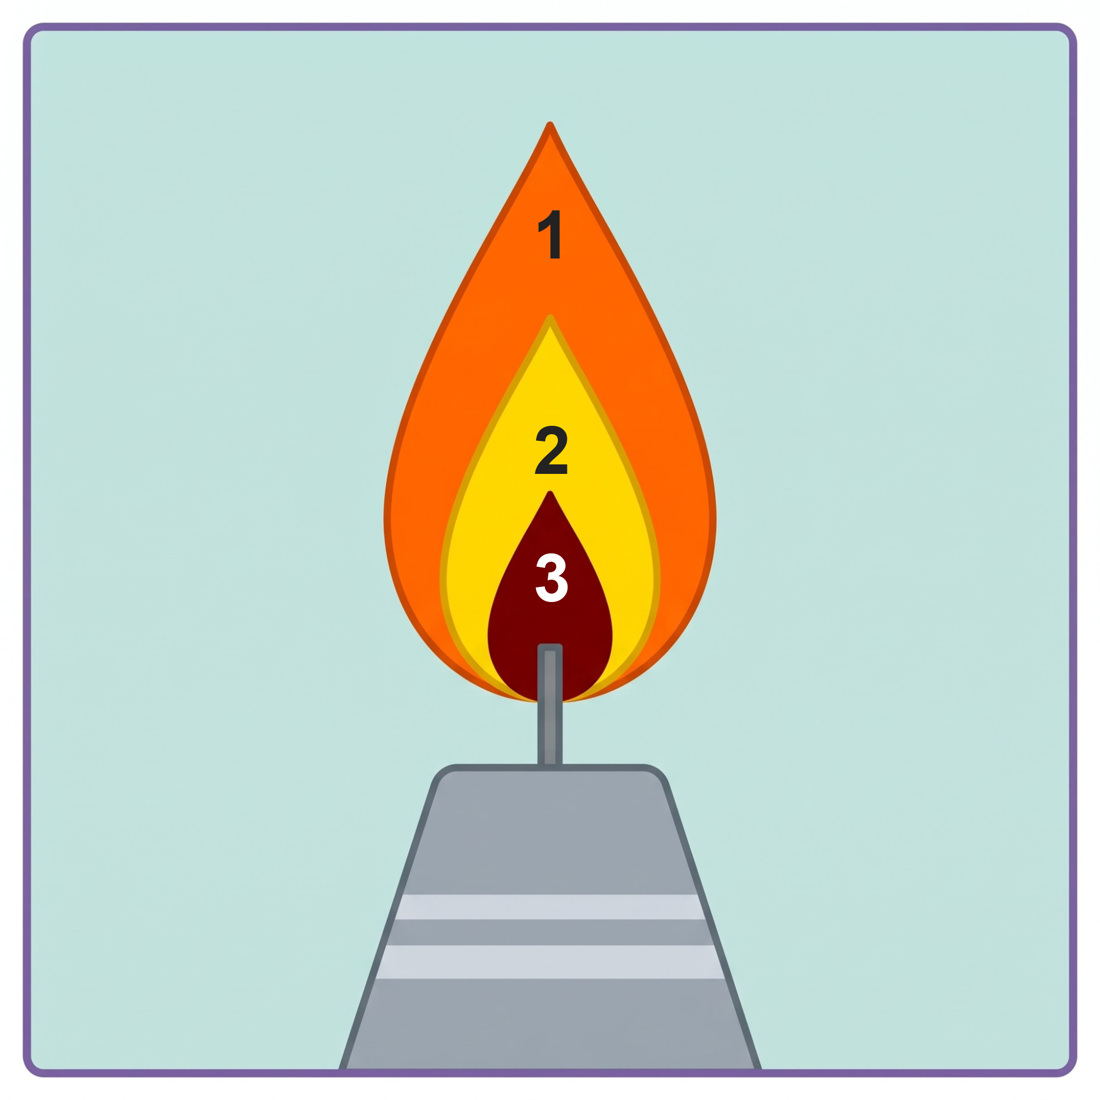
\includegraphics[width=0.86\linewidth]{rasmlar/darslik/d_alanga.png}\end{center}

\noindent\begin{tabular}{@{}p{0.47\linewidth}@{}p{0.47\linewidth}@{}}
A)~\textsl{hamma qismi bir xil} & B)~\textsl{3 -- pastki qism} \\
C)~\textsl{2 -- o`rta qism} & D)~\textsl{1 -- yuqori qism   ---} \\
\end{tabular}\par
\qsep
\end{multicols}
\medskip
\noindent\setlength{\fboxsep}{0pt}\fbox{\begin{tabular}{p{0.74\linewidth}|p{0.2\linewidth}}
\parbox[t]{0.72\linewidth}{\vspace{3pt}\textbf{Topshiriqlar (33--35) va javob variant (A--F)larini o`zaro to`g`ri moslashtiring.} Metan (CH\textsubscript{4}) va propen (C\textsubscript{3}H\textsubscript{6}) dan iborat 7,84 l (n.sh.) aralashma bromli suvdan o`tkazilganda 8 g brom yutildi.
\vspace{3pt}} & \parbox[t]{0.19\linewidth}{\vspace{3pt}A~\textsl{88}\\[3pt]
B~\textsl{11,43}\\[3pt]
C~\textsl{21,43}\\[3pt]
D~\textsl{14,29}\\[3pt]
E~\textsl{1,12}\\[3pt]
F~\textsl{176}}\\ \hline
\parbox[t]{0.72\linewidth}{\vspace{2pt}\textbf{33. Aralashmadagi propen (C\textsubscript{3}H\textsubscript{6}) hajmini (l, n.sh.) aniqlang.}\vspace{2pt}} & \\ \hline
\parbox[t]{0.72\linewidth}{\vspace{2pt}\textbf{34. Aralashmadagi propen (C\textsubscript{3}H\textsubscript{6}) hajmiy ulushini (\%) aniqlang.}\vspace{2pt}} & \\ \hline
\parbox[t]{0.72\linewidth}{\vspace{2pt}\textbf{35. Aralashmani to`liq yoqish uchun zarur havo hajmini (l, n.sh.; havoda 21\% kislorod bor) aniqlang.}\vspace{2pt}} & 
\end{tabular}}
\par\bigskip
\noindent\qn{36.} KMnO\textsubscript{4} + K\textsubscript{2}SO\textsubscript{3} + H\textsubscript{2}O $\to$ MnO\textsubscript{2} + K\textsubscript{2}SO\textsubscript{4} + KOH reaksiya tenglamasini tenglang va barcha koeffitsiyentlar \textbf{yig`indisini aniqlang.}
\javob\qsep
\noindent\qn{37.} 50 g CaCO\textsubscript{3} reaksiyaga kirishdi (CaCO\textsubscript{3} + 2HCl $\to$ CaCl\textsubscript{2} + CO\textsubscript{2} + H\textsubscript{2}O). Ajralgan CO\textsubscript{2} \textbf{hajmini (l, n.sh.) hisoblang.}
\javob\qsep
\noindent\qn{38.} 75,2 g Cu(NO\textsubscript{3})\textsubscript{2} qizdirilganda qisman parchalandi, qattiq qoldiq massasi 53,6 g bo`ldi. Ajralgan gazlar (n.sh.) \textbf{hajmini (l) hisoblang.}
\javob\qsep
\noindent\qn{39.} Etilen va asetilendan iborat 5,6 l (n.sh.) aralashma bromli suvdan o`tkazilganda 56 g brom yutildi. Aralashmadagi asetilenning \textbf{hajmini (l, n.sh.) toping.}
\javob\qsep
\noindent\qn{40.} 14,8 g HCOOC\textsubscript{2}H\textsubscript{5} mo`l NaOH bilan to`liq gidrolizlandi. Hosil bo`lgan spirt \textbf{massasini (g) aniqlang.}
\javob\qsep
\par\bigskip\begin{center}\textbf{\fontsize{13}{15}\selectfont YOZMA ISH}\end{center}
\noindent\qn{41.} \textbf{Topshiriqni bajarish jarayonida barcha reaksiya tenglamalarini yozing. Miqdoriy va arifmetik hisoblashlarni (unga asos bo`lgan usul yoki formulani ko`rsatgan holda) uzviy ketma-ketlikda bajaring.}\par\smallskip
Quyidagi eritmalar berilgan: HCl ning 0,02 mol/l li eritmasi va NaOH ning 0,01 mol/l li eritmasi. Ularni aralashtirib, umumiy hajmi 1 l bo`lgan eritma tayyorlandi (0,3 l HCl eritmasi va 0,7 l NaOH eritmasi). Shuningdek, sirka kislotaning 0,1 mol/l li eritmasida dissotsilanish darajasi 1\%.\par
\noindent 1)\ Aralashtirilgandan keyingi eritmaning pH ini aniqlang.\par
\noindent 2)\ Dastlabki HCl eritmasining pH ini hisoblang. 1 l shu eritmadagi HCl massasini (g) ham hisoblang.\par
\noindent 3)\ Dastlabki NaOH eritmasining pH ini hisoblang.\par
\noindent 4)\ Sirka kislota eritmasidagi H\textsuperscript{+} ionlari konsentratsiyasini (mol/l) va pH ni aniqlang (lg 2 = 0,3, lg 5 = 0,7 ni ishlating). Shuningdek NaOH eritmasi 100 marta suyultirilsa pH qancha bo`ladi?\par
\noindent 5)\ Sirka kislotaning dissotsilanish konstantasini hisoblang (K = C$\alpha$\textsuperscript{2}/(1 $-$ $\alpha$)). Shuningdek HCl eritmasi 10 marta suyultirilsa pH necha bo`ladi?\par
\diqqat{Mazkur topshiriq kengaytirilgan javobni talab etib, uning yechilish usuli va shu usul asosidagi barcha hisoblash amallari javoblar varaqasida aks etishi lozim.}\qsep
\noindent\qn{42.} Quyidagi o`zgarishlar zanjirida \textit{X}, \textit{Y}, \textit{Z} noma'lum organik moddalar:\par
\[\setlength{\fboxsep}{0pt}\text{CH\textsubscript{3}Cl}\xrightarrow{\text{Na}}\text{\textit{X}}\xrightarrow{\text{Cl\textsubscript{2}, yorug`lik}}\text{\textit{Y}}\xrightarrow{\text{KOH (suvli)}}\text{\textit{Z}}\xrightarrow{\text{CuO, t\textdegree{}}}\text{CH\textsubscript{3}CHO}\]
\noindent 1)\ CH\textsubscript{3}Cl $\to$ \textit{X} : reaksiya tenglamasini yozing; hosil bo`lgan moddani nomlang.\par
\noindent 2)\ \textit{X} $\to$ \textit{Y} : reaksiya tenglamasini yozing; hosil bo`lgan moddani nomlang.\par
\noindent 3)\ \textit{Y} $\to$ \textit{Z} : reaksiya tenglamasini yozing; hosil bo`lgan moddani nomlang.\par
\noindent 4)\ \textit{Z} $\to$ CH\textsubscript{3}CHO : reaksiya tenglamasini yozing; hosil bo`lgan moddani nomlang.\par
\diqqat{Mazkur topshiriq kengaytirilgan javobni talab etib, uning yechilish usuli va shu usul asosidagi barcha hisoblash amallari javoblar varaqasida aks etishi lozim.}\qsep
\noindent\qn{43.} \textbf{Topshiriqni bajarish jarayonida barcha reaksiya tenglamalarini yozing. Miqdoriy va arifmetik hisoblashlarni (unga asos bo`lgan usul yoki formulani ko`rsatgan holda) uzviy ketma-ketlikda bajaring.}\par\smallskip
Magniy (Mg) va rux (Zn) dan iborat 15,4 g qotishma mo`l suyultirilgan sulfat kislotada eritildi, bunda 6,72 l (n.sh.) gaz ajraldi. Hosil bo`lgan eritmaga mo`l NaOH eritmasi qo`shildi, hosil bo`lgan cho`kma ajratib olindi va havoda qizdirib quritildi.\par
\noindent 1)\ Reaksiya tenglamalarini yozing va qotishmadagi har bir metallning massasini (g) aniqlang.\par
\noindent 2)\ Qotishmadagi Mg ning massa ulushini (\%) hisoblang.\par
\noindent 3)\ Eritish uchun sarflangan 20\% li H\textsubscript{2}SO\textsubscript{4} eritmasining massasini (g) aniqlang.\par
\noindent 4)\ Mo`l NaOH qo`shilganda hosil bo`lgan cho`kmaning formulasi va massasini (g) toping (reaksiya tenglamalarini yozing).\par
\noindent 5)\ Cho`kma havoda to`liq qizdirilganda hosil bo`lgan oksidning massasini (g) hisoblang.\par
\diqqat{Mazkur topshiriq kengaytirilgan javobni talab etib, uning yechilish usuli va shu usul asosidagi barcha hisoblash amallari javoblar varaqasida aks etishi lozim.}\qsep
\newpage
\renewcommand{\curvar}{17-variant}
\thispagestyle{first}
\noindent\textit{Davriy jadvaldan foydalanish mumkin.}
\par\smallskip
\begin{multicols}{2}
\noindent\qn{1.} 3 mol Na\textsubscript{2}SO\textsubscript{4} va 2 mol K\textsubscript{3}PO\textsubscript{4} suvda eritilib, eritma hajmi 5 l ga yetkazildi. Eritmadagi barcha ionlarning umumiy molyar \textbf{konsentratsiyasini (mol/l) aniqlang} (kuchli elektrolitlar to`liq dissotsilanadi).

\noindent A)~\textsl{3,4} \hfill B)~\textsl{1} \hfill C)~\textsl{6,8} \hfill D)~\textsl{1,7}\par
\qsep
\noindent\qn{2.} 13,12 l He 127 \textdegree{}C va 1 atm bosimda necha gramm keladi? (R = 0,082 l$\cdot$atm/(mol$\cdot$K))

\noindent A)~\textsl{3,2} \hfill B)~\textsl{1,6} \hfill C)~\textsl{0,8} \hfill D)~\textsl{2,34}\par
\qsep
\noindent\qn{3.} 1 M Al\textsubscript{2}(SO\textsubscript{4})\textsubscript{3} eritmasining normal \textbf{konsentratsiyasini (n) aniqlang.}

\noindent A)~\textsl{1} \hfill B)~\textsl{12} \hfill C)~\textsl{0,167} \hfill D)~\textsl{6}\par
\qsep
\noindent\qn{4.} Quyidagi tuzlarning qaysilari suvli eritmasi kislotali muhitga ega? 1) Na\textsubscript{2}CO\textsubscript{3}; 2) ZnCl\textsubscript{2}; 3) CuSO\textsubscript{4}; 4) K\textsubscript{2}S

\noindent A)~\textsl{3, 4} \hfill B)~\textsl{2, 3} \hfill C)~\textsl{1, 3, 4} \hfill D)~\textsl{4}\par
\qsep
\noindent\qn{5.} Jadvalda bog`lar hosil qiluvchi atomlarning elektrmanfiyliklari berilgan:
\begin{center}
\renewcommand{\arraystretch}{1.15}
\fitbox{\begin{tabular}{|c|c|c|}\hline
\textbf{Bog`} & \textbf{EM (1-atom)} & \textbf{EM (2-atom)} \\ \hline
C--H & 2,5 & 2,1 \\ \hline
K--Br & 0,8 & 2,8 \\ \hline
N--H & 3 & 2,1 \\ \hline
Si--O & 1,8 & 3,5 \\ \hline
\end{tabular}}
\end{center}
Qaysi bog` eng qutbli (eng ko`p ionli xarakterga ega)?

\noindent A)~\textsl{C--H} \hfill B)~\textsl{N--H} \hfill C)~\textsl{Si--O} \hfill D)~\textsl{K--Br}\par
\qsep
\noindent\qn{6.} 29,25 g NaCl 250 g suvda eritildi. Eritmaning molyal \textbf{konsentratsiyasini (mol/kg) aniqlang.}

\noindent A)~\textsl{1,79} \hfill B)~\textsl{0} \hfill C)~\textsl{4} \hfill D)~\textsl{2}\par
\qsep
\noindent\qn{7.} Rasmda indikatorlarning pH ga bog`liq rangi ko`rsatilgan.
\begin{center}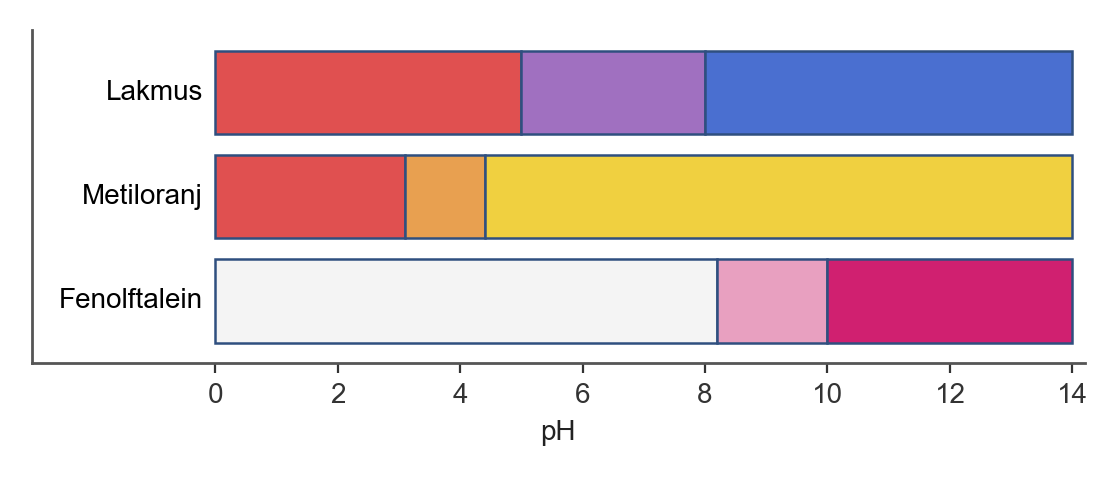
\includegraphics[width=0.86\linewidth]{rasmlar/gen/in_47359.png}\end{center}
pH = 13 bo`lgan eritmada metiloranj qanday rangga kiradi?

\noindent\begin{tabular}{@{}p{0.47\linewidth}@{}p{0.47\linewidth}@{}}
A)~\textsl{sariq} & B)~\textsl{qizil} \\
C)~\textsl{malina rang} & D)~\textsl{rangsiz} \\
\end{tabular}\par
\qsep
\noindent\qn{8.} Laboratoriyada KBr eritmalari quyidagicha tayyorlangan:
\begin{center}
\renewcommand{\arraystretch}{1.15}
\fitbox{\begin{tabular}{|c|c|c|}\hline
\textbf{Idish} & \textbf{Eritma massasi, g} & \textbf{$\omega$(KBr), \%} \\ \hline
A & 100 & 20 \\ \hline
B & 100 & 40 \\ \hline
\end{tabular}}
\end{center}
Bu ikki eritma bir idishga quyilib va ustiga 50 g suv qo`shilsa, yangi eritmadagi KBr ning massa ulushi (\%) qancha bo`ladi?

\noindent A)~\textsl{30} \hfill B)~\textsl{24} \hfill C)~\textsl{60} \hfill D)~\textsl{21,6}\par
\qsep
\noindent\qn{9.} Quyidagi jadvalda KNO\textsubscript{3} tuzining eritmalari keltirilgan:
\begin{center}
\renewcommand{\arraystretch}{1.15}
\fitbox{\begin{tabular}{|c|c|c|}\hline
\textbf{No.} & \textbf{m(eritma), g} & \textbf{$\omega$, \%} \\ \hline
I & 100 & 20 \\ \hline
II & 150 & 25 \\ \hline
\end{tabular}}
\end{center}
Eritmalar aralashtirildi. Oxirgi eritmadagi tuzning massa \textbf{ulushini (\%) toping.}

\noindent A)~\textsl{22,5} \hfill B)~\textsl{45} \hfill C)~\textsl{23} \hfill D)~\textsl{22}\par
\qsep
\noindent\qn{10.} Elementning massa-spektri (izotoplar tarqalganligi) berilgan.
\begin{center}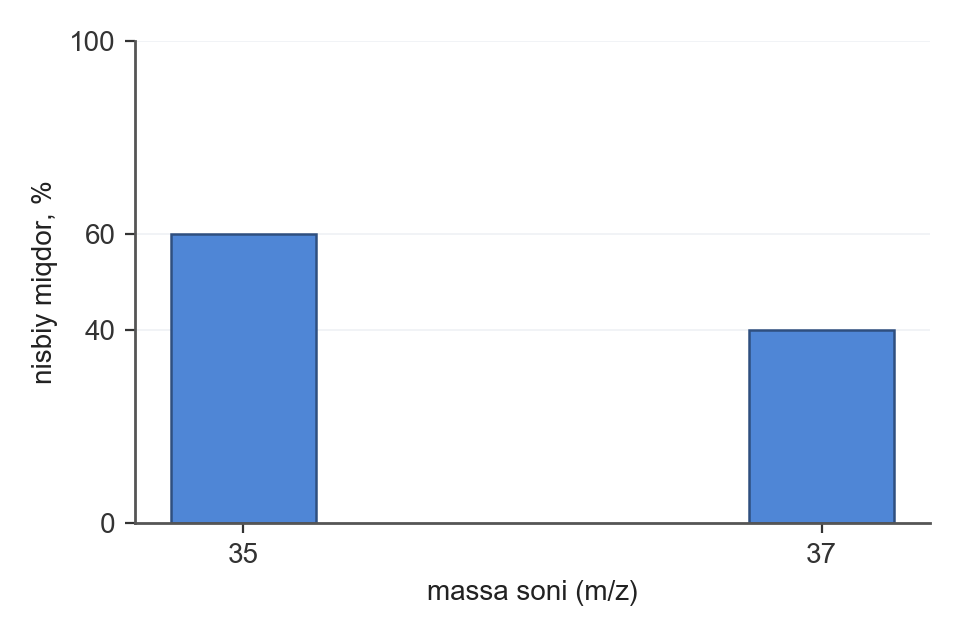
\includegraphics[width=0.86\linewidth]{rasmlar/gen/ms_v17_0.png}\end{center}
Elementning o`rtacha nisbiy atom \textbf{massasini aniqlang.}

\noindent A)~\textsl{36} \hfill B)~\textsl{36,2} \hfill C)~\textsl{35,8} \hfill D)~\textsl{35}\par
\qsep
\noindent\qn{11.} 32,8 l O\textsubscript{2} 127 \textdegree{}C va 0,5 atm bosimda necha gramm keladi? (R = 0,082 l$\cdot$atm/(mol$\cdot$K))

\noindent A)~\textsl{32} \hfill B)~\textsl{8} \hfill C)~\textsl{16} \hfill D)~\textsl{46,86}\par
\qsep
\noindent\qn{12.} Al + HNO\textsubscript{3} $\to$ Al(NO\textsubscript{3})\textsubscript{3} + NO + H\textsubscript{2}O reaksiyasida 1 mol Al erisa, HNO\textsubscript{3} ning necha moli oksidlovchi vazifasini bajaradi?

\noindent A)~\textsl{1} \hfill B)~\textsl{4} \hfill C)~\textsl{3} \hfill D)~\textsl{2}\par
\qsep
\noindent\qn{13.} 40 l C\textsubscript{2}H\textsubscript{2} va 240 l H\textsubscript{2} aralashmasi C\textsubscript{2}H\textsubscript{2} + 2H\textsubscript{2} $\to$ C\textsubscript{2}H\textsubscript{6} tenglama bo`yicha to`liq reaksiyaga kirishdi (barcha gazlar bir xil sharoitda o`lchandi). Aralashma hajmi necha litrga o`zgargan (modul bo`yicha)?

\noindent A)~\textsl{280} \hfill B)~\textsl{80} \hfill C)~\textsl{200} \hfill D)~\textsl{40}\par
\qsep
\noindent\qn{14.} KNO\textsubscript{3} tarkibidagi kaliy ning massa \textbf{ulushini (\%) aniqlang.}

\noindent A)~\textsl{38,6} \hfill B)~\textsl{19,3} \hfill C)~\textsl{77,2} \hfill D)~\textsl{2,6}\par
\qsep
\noindent\qn{15.} 17 g NaNO\textsubscript{3} to`liq parchalanguncha qizdirildi. Qattiq qoldiq \textbf{massasini (g) aniqlang.}

\noindent A)~\textsl{17} \hfill B)~\textsl{27,6} \hfill C)~\textsl{6,9} \hfill D)~\textsl{13,8}\par
\qsep
\noindent\qn{16.} H\textsubscript{2}S + CuSO\textsubscript{4} $\to$ CuS + H\textsubscript{2}SO\textsubscript{4} jarayoni uchun 4,48 l (n.sh.) H\textsubscript{2}S olingan (unum 60\%). CuS \textbf{miqdorini (mol) aniqlang.}

\noindent A)~\textsl{0,2} \hfill B)~\textsl{0,24} \hfill C)~\textsl{0,06} \hfill D)~\textsl{0,12}\par
\qsep
\noindent\qn{17.} Reaksiya tenglamasi: 2Cu(NO\textsubscript{3})\textsubscript{2} $\to$ 2CuO + 4NO\textsubscript{2} + O\textsubscript{2}. Reaksiyaga tarkibida 60\% aralashma bo`lgan 117,5 g namuna (asosiy modda Cu(NO\textsubscript{3})\textsubscript{2}) kirishdi. O\textsubscript{2} \textbf{hajmini (l, n.sh.) hisoblang.}

\noindent A)~\textsl{2,8} \hfill B)~\textsl{11,2} \hfill C)~\textsl{5,6} \hfill D)~\textsl{1,4}\par
\qsep
\noindent\qn{18.} 3,1 g fosfor yondirilib, hosil bo`lgan oksid suvda eritildi (ortofosfat kislota), so`ng 0,2 mol NaOH qo`shildi. Hosil bo`lgan Na\textsubscript{2}HPO\textsubscript{4} \textbf{massasini (g) aniqlang.}

\noindent A)~\textsl{28,4} \hfill B)~\textsl{14,2} \hfill C)~\textsl{7,1} \hfill D)~\textsl{12}\par
\qsep
\noindent\qn{19.} 2KClO\textsubscript{3} $\to$ 2KCl + 3O\textsubscript{2} reaksiyasida 122,5 g KClO\textsubscript{3} ishtirok etdi (unum 75\%). O\textsubscript{2} \textbf{hajmini (l, n.sh.) toping.}

\noindent A)~\textsl{25,2} \hfill B)~\textsl{14,93} \hfill C)~\textsl{50,4} \hfill D)~\textsl{12,6}\par
\qsep
\noindent\qn{20.} C\textsubscript{2}H\textsubscript{6} + Cl\textsubscript{2} $\to$ C\textsubscript{2}H\textsubscript{5}Cl + HCl jarayoni uchun 22,4 l (n.sh.) C\textsubscript{2}H\textsubscript{6} olingan (unum 75\%). HCl \textbf{hajmini (l, n.sh.) aniqlang.}

\noindent A)~\textsl{22,4} \hfill B)~\textsl{33,6} \hfill C)~\textsl{16,8} \hfill D)~\textsl{8,4}\par
\qsep
\noindent\qn{21.} CH\textsubscript{3}--CH\textsubscript{2}--CH(CH\textsubscript{3})--CH\textsubscript{2}--CH\textsubscript{3} birikmaning sistematik nomi qaysi qatorda to`g`ri keltirilgan?

\noindent\begin{tabular}{@{}p{0.47\linewidth}@{}p{0.47\linewidth}@{}}
A)~\textsl{2-etilbutan} & B)~\textsl{3-metilpentan} \\
C)~\textsl{2-metilpentan} & D)~\textsl{3-etilbutan} \\
\end{tabular}\par
\qsep
\noindent\qn{22.} Arenlar, neft va tabiiy gaz haqida qaysi fikrlar to`g`ri? 1) Benzoldan nitrobenzol nitrolash bilan olinadi; 2) Benzol bromli suvni rangsizlantirmaydi; 3) Benzol uchun birikish reaksiyalari mutlaqo xos emas; 4) Benzolda 6 ta sp\textsuperscript{2} gibridlangan uglerod bor

\noindent A)~\textsl{2, 3} \hfill B)~\textsl{3, 4} \hfill C)~\textsl{1, 2, 4} \hfill D)~\textsl{1, 2, 3}\par
\qsep
\noindent\qn{23.} C\textsubscript{2}H\textsubscript{2} + H\textsubscript{2}O (Hg\textsuperscript{2+}) reaksiyasi natijasida qaysi organik modda hosil bo`ladi?

\noindent\begin{tabular}{@{}p{0.47\linewidth}@{}p{0.47\linewidth}@{}}
A)~\textsl{etilatsetat} & B)~\textsl{asetilen} \\
C)~\textsl{sirka aldegid} & D)~\textsl{etanol} \\
\end{tabular}\par
\qsep
\noindent\qn{24.} Aldegid va ketonlar haqida qaysi fikrlar to`g`ri? 1) Aldegidlar qaytarilganda ikkilamchi spirt hosil bo`ladi; 2) Ketonlar kuchsiz oksidlovchilar bilan oksidlanmaydi; 3) Formaldegid gaz holatda, suvda yaxshi eriydi; 4) Aldegidlar "kumush ko`zgu" reaksiyasini beradi

\noindent A)~\textsl{1, 2, 3} \hfill B)~\textsl{3, 4} \hfill C)~\textsl{2, 3} \hfill D)~\textsl{2, 3, 4}\par
\qsep
\noindent\qn{25.} 14,8 g propion kislotani neytrallash uchun 10\% li NaOH eritmasidan necha gramm kerak?

\noindent A)~\textsl{8} \hfill B)~\textsl{80} \hfill C)~\textsl{40} \hfill D)~\textsl{148}\par
\qsep
\noindent\qn{26.} Murakkab efirlar va yog`lar haqida qaysi fikrlar to`g`ri? 1) Sovun --- yuqori yog` kislotalarning natriyli tuzi; 2) Yog`lar glitserin va yuqori yog` kislotalarning murakkab efirlari; 3) Suyuq yog`lar to`yinmagan kislotalardan hosil bo`lgan; 4) Dietil efir spirtdan yuqori haroratda qaynaydi

\noindent A)~\textsl{1, 2, 3} \hfill B)~\textsl{2, 3, 4} \hfill C)~\textsl{1, 4} \hfill D)~\textsl{1, 3, 4}\par
\qsep
\noindent\qn{27.} Reaksiya tenglamasi: C\textsubscript{6}H\textsubscript{12}O\textsubscript{6} $\to$ 2C\textsubscript{2}H\textsubscript{5}OH + 2CO\textsubscript{2}. Reaksiyaga 72 g C\textsubscript{6}H\textsubscript{12}O\textsubscript{6} kirishdi. CO\textsubscript{2} \textbf{hajmini (l, n.sh.) hisoblang.}

\noindent A)~\textsl{4,48} \hfill B)~\textsl{35,84} \hfill C)~\textsl{17,92} \hfill D)~\textsl{8,96}\par
\qsep
\noindent\qn{28.} Aminlar, aminokislotalar va oqsillar haqida qaysi fikrlar to`g`ri? 1) Oqsillar biuret reaksiyasini beradi; 2) Aminokislotalar amfoter birikmalar; 3) Anilin bromli suv bilan oq cho`kma beradi; 4) Glitsin optik faol

\noindent A)~\textsl{1, 4} \hfill B)~\textsl{1, 2} \hfill C)~\textsl{2, 3} \hfill D)~\textsl{1, 2, 3}\par
\qsep
\noindent\qn{29.} Reaksiya tenglamasi: C\textsubscript{3}H\textsubscript{6} + H\textsubscript{2} $\to$ C\textsubscript{3}H\textsubscript{8}. Reaksiyaga 5,6 l (n.sh.) C\textsubscript{3}H\textsubscript{6} kirishdi. C\textsubscript{3}H\textsubscript{8} \textbf{hajmini (l, n.sh.) hisoblang.}

\noindent A)~\textsl{5,6} \hfill B)~\textsl{11,2} \hfill C)~\textsl{2,8} \hfill D)~\textsl{8,4}\par
\qsep
\noindent\qn{30.} Kimyoviy laboratoriyada ajratgich voronka nima uchun ishlatiladi?
\noindent A)~\textsl{probirkani qizdirish}\par
\noindent B)~\textsl{eritmaning kichik hajmlarini o`lchab olish}\par
\noindent C)~\textsl{gaz (H\textsubscript{2}, CO\textsubscript{2}, H\textsubscript{2}S) olish}\par
\noindent D)~\textsl{aralashmaydigan suyuqliklarni ajratish}\par
\qsep
\noindent\qn{31.} Kimyo laboratoriyasida ishlash qoidalari haqida qaysi fikrlar to`g`ri? 1) Reaktivlarni tatib ko`rish mumkin; 2) Zaharli gaz ajraladigan tajriba mo`rili shkafda o`tkaziladi; 3) Spirt lampa boshqa lampadan yoqilmaydi; 4) Probirka qizdirilganda og`zi odamga qaratilmaydi

\noindent A)~\textsl{1, 2} \hfill B)~\textsl{3, 4} \hfill C)~\textsl{2, 3, 4} \hfill D)~\textsl{1, 3, 4}\par
\qsep
\noindent\qn{32.} Rasmdagi tajribada cho`g`langan yog`och konsentrlangan HNO\textsubscript{3} bug`lari ichida yonmoqda. Bu jarayonda HNO\textsubscript{3} qanday vazifani bajaradi?
\begin{center}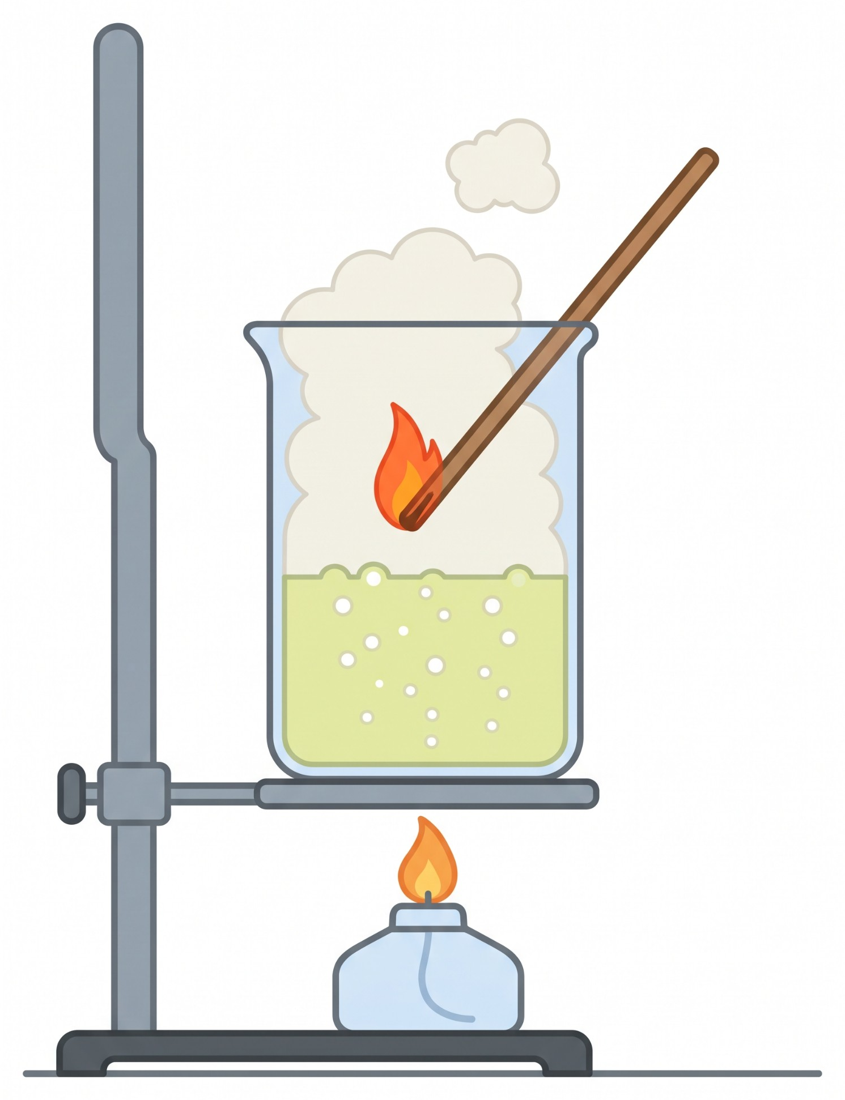
\includegraphics[width=0.86\linewidth]{rasmlar/darslik/d_hno3_yogoch.png}\end{center}

\noindent\begin{tabular}{@{}p{0.47\linewidth}@{}p{0.47\linewidth}@{}}
A)~\textsl{qaytaruvchi} & B)~\textsl{oksidlovchi} \\
C)~\textsl{katalizator} & D)~\textsl{erituvchi   ---} \\
\end{tabular}\par
\qsep
\end{multicols}
\medskip
\noindent\setlength{\fboxsep}{0pt}\fbox{\begin{tabular}{p{0.74\linewidth}|p{0.2\linewidth}}
\parbox[t]{0.72\linewidth}{\vspace{3pt}\textbf{Topshiriqlar (33--35) va javob variant (A--F)larini o`zaro to`g`ri moslashtiring.} Temir va alyuminiy (Fe va Al) dan iborat 6,85 g qotishma mo`l HCl eritmasida eritilganda 6,16 l (n.sh.) gaz ajraldi.
\vspace{3pt}} & \parbox[t]{0.19\linewidth}{\vspace{3pt}A~\textsl{150,56}\\[3pt]
B~\textsl{100,38}\\[3pt]
C~\textsl{81,75}\\[3pt]
D~\textsl{200,75}\\[3pt]
E~\textsl{40,88}\\[3pt]
F~\textsl{26,38}}\\ \hline
\parbox[t]{0.72\linewidth}{\vspace{2pt}\textbf{33. Qotishmadagi Fe massa ulushini (\%) aniqlang.}\vspace{2pt}} & \\ \hline
\parbox[t]{0.72\linewidth}{\vspace{2pt}\textbf{34. Reaksiya uchun sarflangan 20\% li HCl massasini (g) aniqlang.}\vspace{2pt}} & \\ \hline
\parbox[t]{0.72\linewidth}{\vspace{2pt}\textbf{35. Eritmadagi tuzlarning umumiy massasini (g) aniqlang.}\vspace{2pt}} & 
\end{tabular}}
\par\bigskip
\noindent\qn{36.} Mg + H\textsubscript{2}SO\textsubscript{4} $\to$ MgSO\textsubscript{4} + H\textsubscript{2}S + H\textsubscript{2}O reaksiya tenglamasini tenglang va barcha koeffitsiyentlar \textbf{yig`indisini aniqlang.}
\javob\qsep
\noindent\qn{37.} 8,5 g H\textsubscript{2}O\textsubscript{2} reaksiyaga kirishdi (2H\textsubscript{2}O\textsubscript{2} $\to$ 2H\textsubscript{2}O + O\textsubscript{2}). Ajralgan O\textsubscript{2} \textbf{hajmini (l, n.sh.) hisoblang} (unum 75\%).
\javob\qsep
\noindent\qn{38.} NaBr va NaI dan iborat 17,8 g aralashma eritilib, mo`l xlor o`tkazildi, eritma bug`latilib quruq qoldiq 8,78 g chiqdi. Aralashmadagi NaI ning \textbf{massasini (g) toping.}
\javob\qsep
\noindent\qn{39.} Etilen va asetilendan iborat 3,36 l (n.sh.) aralashma bromli suvdan o`tkazilganda 32 g brom yutildi. Aralashmadagi asetilenning \textbf{hajmini (l, n.sh.) toping.}
\javob\qsep
\noindent\qn{40.} 80,6 g tripalmitin gidrolizlanganda necha gramm glitserin hosil bo`ladi?
\javob\qsep
\par\bigskip\begin{center}\textbf{\fontsize{13}{15}\selectfont YOZMA ISH}\end{center}
\noindent\qn{41.} \textbf{Topshiriqni bajarish jarayonida barcha reaksiya tenglamalarini yozing. Miqdoriy va arifmetik hisoblashlarni (unga asos bo`lgan usul yoki formulani ko`rsatgan holda) uzviy ketma-ketlikda bajaring.}\par\smallskip
Tarkibida 2 mol H\textsubscript{2}SO\textsubscript{4} va 0,25 mol SO\textsubscript{3} bo`lgan oleum namunasi 200 g suvda eritildi.\par
\noindent 1)\ Oleumdagi SO\textsubscript{3} ning massa ulushini (\%) hisoblang.\par
\noindent 2)\ SO\textsubscript{3} suv bilan reaksiyaga kirishgandan so`ng eritmadagi H\textsubscript{2}SO\textsubscript{4} ning umumiy miqdorini (mol) toping (reaksiya tenglamasini yozing). Hosil bo`lgan eritmadagi suvning massasini (g) ham hisoblang.\par
\noindent 3)\ Hosil bo`lgan eritmadagi H\textsubscript{2}SO\textsubscript{4} ning massa ulushini (\%) aniqlang.\par
\noindent 4)\ Shu eritmani to`liq neytrallash uchun zichligi 1,11 g/ml bo`lgan 10\% li NaOH eritmasidan necha ml kerak? Hosil bo`lgan Na\textsubscript{2}SO\textsubscript{4} massasini (g) ham toping.\par
\noindent 5)\ Eritmaga mo`l BaCl\textsubscript{2} eritmasi qo`shilganda hosil bo`ladigan cho`kma massasini (g) toping. Hosil bo`lgan eritmaning zichligi 1,4 g/ml bo`lsa, uning molyar konsentratsiyasini (mol/l) toping.\par
\diqqat{Mazkur topshiriq kengaytirilgan javobni talab etib, uning yechilish usuli va shu usul asosidagi barcha hisoblash amallari javoblar varaqasida aks etishi lozim.}\qsep
\noindent\qn{42.} Quyidagi o`zgarishlar zanjirida \textit{X}, \textit{Y}, \textit{Z} noma'lum organik moddalar:\par
\[\setlength{\fboxsep}{0pt}\text{C\textsubscript{2}H\textsubscript{5}OH}\xrightarrow{\text{CuO, t\textdegree{}}}\text{\textit{X}}\xrightarrow{\text{Ag\textsubscript{2}O, NH\textsubscript{3}}}\text{\textit{Y}}\xrightarrow{\text{Cl\textsubscript{2}, P}}\text{ClCH\textsubscript{2}COOH}\]
\noindent 1)\ C\textsubscript{2}H\textsubscript{5}OH $\to$ \textit{X} : reaksiya tenglamasini yozing; hosil bo`lgan moddani nomlang.\par
\noindent 2)\ \textit{X} $\to$ \textit{Y} : reaksiya tenglamasini yozing; hosil bo`lgan moddani nomlang.\par
\noindent 3)\ \textit{Y} $\to$ ClCH\textsubscript{2}COOH : reaksiya tenglamasini yozing; hosil bo`lgan moddani nomlang.\par
\diqqat{Mazkur topshiriq kengaytirilgan javobni talab etib, uning yechilish usuli va shu usul asosidagi barcha hisoblash amallari javoblar varaqasida aks etishi lozim.}\qsep
\noindent\qn{43.} \textbf{Topshiriqni bajarish jarayonida barcha reaksiya tenglamalarini yozing. Miqdoriy va arifmetik hisoblashlarni (unga asos bo`lgan usul yoki formulani ko`rsatgan holda) uzviy ketma-ketlikda bajaring.}\par\smallskip
Alyuminiy, temir va misdan iborat 11,5 g aralashma mo`l NaOH eritmasi bilan reaksiyaga kirishganda 3,36 l (n.sh.) vodorod ajraldi. Xuddi shunday tarkibli ikkinchi aralashma (11,5 g) mo`l xlorid kislota bilan reaksiyaga kirishganda 5,6 l (n.sh.) vodorod ajraldi (temir FeCl\textsubscript{2} ga o`tdi).\par
\noindent 1)\ Aralashmadagi har bir metallning massasini (g) va massa ulushini (\%) aniqlang (reaksiya tenglamalarini yozing).\par
\noindent 2)\ Xlorid kislota bilan reaksiyadan keyin qolgan qoldiq konsentrlangan HNO\textsubscript{3} da to`liq eritildi. Ajralgan gazning hajmini (l, n.sh.) aniqlang.\par
\noindent 3)\ Xlorid kislota bilan olingan eritmaga mo`l NaOH qo`shildi, hosil bo`lgan cho`kma ajratib olinib, havoda to`liq oksidlanguncha qoldirildi. Cho`kma massasini (g) toping.\par
\noindent 4)\ Mis nitrat eritmasi bug`latilib, quruq tuz qizdirilganda hosil bo`ladigan qattiq qoldiq massasini (g) va gazlar aralashmasining hajmini (l, n.sh.) aniqlang.\par
\noindent 5)\ Aralashmadagi alyuminiyni eritish uchun (2Al + 2NaOH + 6H\textsubscript{2}O $\to$ 2Na[Al(OH)\textsubscript{4}] + 3H\textsubscript{2}) 10\% li NaOH eritmasidan necha gramm kerak?\par
\diqqat{Mazkur topshiriq kengaytirilgan javobni talab etib, uning yechilish usuli va shu usul asosidagi barcha hisoblash amallari javoblar varaqasida aks etishi lozim.}\qsep
\newpage
\renewcommand{\curvar}{18-variant}
\thispagestyle{first}
\noindent\textit{Davriy jadvaldan foydalanish mumkin.}
\par\smallskip
\begin{multicols}{2}
\noindent\qn{1.} N\textsubscript{2}O\textsubscript{4} $\rightleftarrows$ 2NO\textsubscript{2} reaksiyasi 1 l hajmli idishda o`tkazildi. Ma'lumotlar jadvalda berilgan:
\begin{center}
\renewcommand{\arraystretch}{1.15}
\fitbox{\begin{tabular}{|c|c|c|}\hline
\textbf{Modda} & \textbf{N\textsubscript{2}O\textsubscript{4}} & \textbf{NO\textsubscript{2}} \\ \hline
Boshlang`ich, mol & 4 & 0 \\ \hline
Muvozanatda, mol & --- & 1 \\ \hline
\end{tabular}}
\end{center}
N\textsubscript{2}O\textsubscript{4} ning necha foizi reaksiyaga \textbf{kirishganini aniqlang.}

\noindent A)~\textsl{12,5} \hfill B)~\textsl{6,2} \hfill C)~\textsl{18,8} \hfill D)~\textsl{87,5}\par
\qsep
\noindent\qn{2.} Rasmda molekulaning sharsimon modeli tasvirlangan (yashil -- C, sariq -- H, qizil -- O, ko`k -- N).
\begin{center}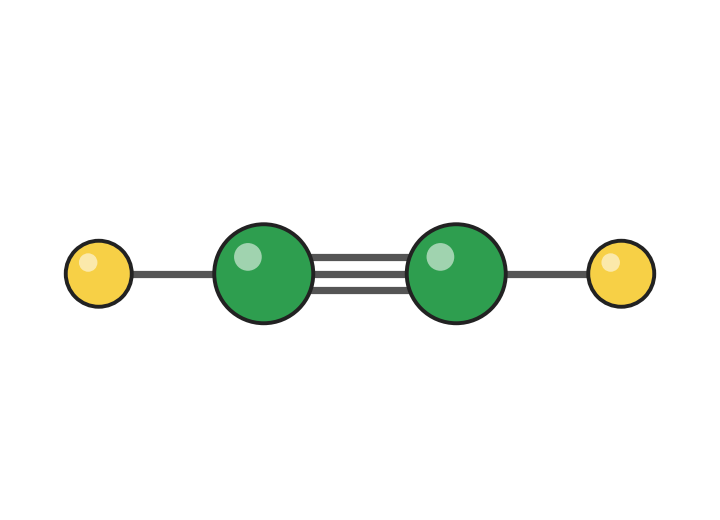
\includegraphics[width=0.86\linewidth]{rasmlar/gen/md_706582.png}\end{center}
Molekula fazoviy shakli qanday?

\noindent\begin{tabular}{@{}p{0.47\linewidth}@{}p{0.47\linewidth}@{}}
A)~\textsl{uchburchakli piramida} & B)~\textsl{burchakli} \\
C)~\textsl{tetraedr} & D)~\textsl{chiziqli} \\
\end{tabular}\par
\qsep
\noindent\qn{3.} H\textsubscript{2}O\textsubscript{2} tarkibida O ning oksidlanish \textbf{darajasini aniqlang.}

\noindent A)~\textsl{$-$2} \hfill B)~\textsl{$-$3 va +5} \hfill C)~\textsl{$-$1} \hfill D)~\textsl{+6}\par
\qsep
\noindent\qn{4.} Na\textsubscript{2}SO\textsubscript{4} eritmasiga 0,5 mol/l li BaCl\textsubscript{2} eritmasi oz-ozdan qo`shilganda hosil bo`lgan cho`kma massasining qo`shilgan hajmga bog`liqligi grafikda keltirilgan.
\begin{center}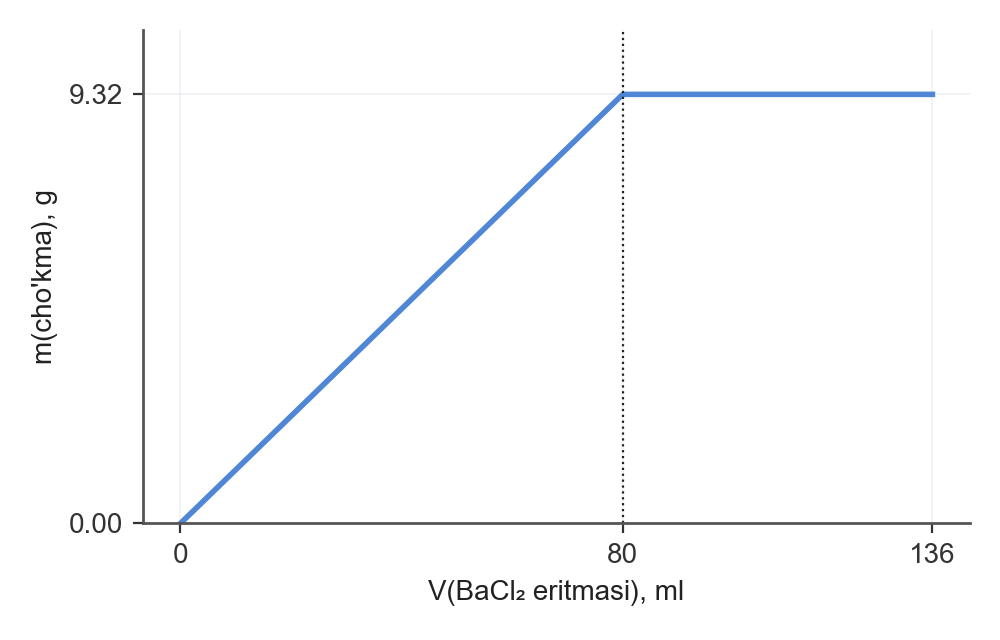
\includegraphics[width=0.86\linewidth]{rasmlar/gen/pp_v18_0.png}\end{center}
Dastlabki eritmadagi Na\textsubscript{2}SO\textsubscript{4} ning \textbf{massasini (g) hisoblang.}

\noindent A)~\textsl{9,32} \hfill B)~\textsl{8,32} \hfill C)~\textsl{5,68} \hfill D)~\textsl{11,36}\par
\qsep
\noindent\qn{5.} 2NO + O\textsubscript{2} $\rightleftarrows$ 2NO\textsubscript{2} reaksiyada muvozanat qaror topganda [NO] = 1, [O\textsubscript{2}] = 1, [NO\textsubscript{2}] = 4 mol/l bo`ldi. NO ning boshlang`ich \textbf{konsentratsiyasini (mol/l) aniqlang.}

\noindent A)~\textsl{5} \hfill B)~\textsl{1} \hfill C)~\textsl{7} \hfill D)~\textsl{3}\par
\qsep
\noindent\qn{6.} Quyidagi jadvalda Na\textsubscript{2}CO\textsubscript{3} tuzining eritmalari keltirilgan:
\begin{center}
\renewcommand{\arraystretch}{1.15}
\fitbox{\begin{tabular}{|c|c|c|}\hline
\textbf{No.} & \textbf{m(eritma), g} & \textbf{$\omega$, \%} \\ \hline
I & 100 & 20 \\ \hline
II & 200 & 30 \\ \hline
\end{tabular}}
\end{center}
Eritmalar aralashtirildi. Oxirgi eritmadagi tuzning massa \textbf{ulushini (\%) toping.}

\noindent A)~\textsl{25} \hfill B)~\textsl{26,67} \hfill C)~\textsl{50} \hfill D)~\textsl{23,33}\par
\qsep
\noindent\qn{7.} 11,2 g Fe va 3,2 g S aralashtirilib, reaksiya o`tkazildi (Fe + S $\to$ FeS). Hosil bo`lgan FeS \textbf{massasini (g) aniqlang.}

\noindent A)~\textsl{17,6} \hfill B)~\textsl{4,4} \hfill C)~\textsl{13,2} \hfill D)~\textsl{8,8}\par
\qsep
\noindent\qn{8.} 8 g NaOH 500 g suvda eritildi. Eritmaning molyal \textbf{konsentratsiyasini (mol/kg) aniqlang.}

\noindent A)~\textsl{0,4} \hfill B)~\textsl{0,39} \hfill C)~\textsl{0} \hfill D)~\textsl{0,8}\par
\qsep
\noindent\qn{9.} Faqat qaytaruvchi bo`la oladigan \textbf{ionlarni aniqlang}: 1) Fe\textsuperscript{3+}; 2) Fe\textsuperscript{2+}; 3) K\textsuperscript{+}; 4) Cl\textsuperscript{$-$}

\noindent A)~\textsl{1} \hfill B)~\textsl{2} \hfill C)~\textsl{1, 3} \hfill D)~\textsl{4}\par
\qsep
\noindent\qn{10.} C\textsubscript{6}H\textsubscript{6} molekulasidagi $\sigma$ va $\pi$ bog`lar \textbf{sonini aniqlang.}

\noindent A)~\textsl{11 va 3} \hfill B)~\textsl{12 va 3} \hfill C)~\textsl{12 va 4} \hfill D)~\textsl{13 va 3}\par
\qsep
\noindent\qn{11.} CH\textsubscript{4} gazining 27 \textdegree{}C va 1 atm bosimdagi \textbf{zichligini (g/l) aniqlang.} (R = 0,082 l$\cdot$atm/(mol$\cdot$K))

\noindent A)~\textsl{1,3} \hfill B)~\textsl{0,33} \hfill C)~\textsl{0,71} \hfill D)~\textsl{0,65}\par
\qsep
\noindent\qn{12.} 3 mol NaCl va 3 mol HNO\textsubscript{3} suvda eritilib, eritma hajmi 4 l ga yetkazildi. Eritmadagi barcha ionlarning umumiy molyar \textbf{konsentratsiyasini (mol/l) aniqlang} (kuchli elektrolitlar to`liq dissotsilanadi).

\noindent A)~\textsl{1,5} \hfill B)~\textsl{6} \hfill C)~\textsl{3} \hfill D)~\textsl{2,25}\par
\qsep
\noindent\qn{13.} Na\textsubscript{2}SO\textsubscript{4} ning suvli eritmasi inert elektrodlar bilan elektroliz qilinganda qaysi moddalar ajraladi?

\noindent A)~\textsl{Ag va O\textsubscript{2}} \hfill B)~\textsl{H\textsubscript{2} va O\textsubscript{2}} \hfill C)~\textsl{Cu va O\textsubscript{2}} \hfill D)~\textsl{Cu va Cl\textsubscript{2}}\par
\qsep
\noindent\qn{14.} Qaysi juftliklar o`zaro reaksiyaga kirishmaydi? 1) Fe\textsubscript{2}O\textsubscript{3} va H\textsubscript{2}O; 2) SiO\textsubscript{2} va H\textsubscript{2}O; 3) Zn va NaOH; 4) NaCl va HNO\textsubscript{3}

\noindent A)~\textsl{3, 4} \hfill B)~\textsl{1, 4} \hfill C)~\textsl{1, 2, 3} \hfill D)~\textsl{1, 2, 4}\par
\qsep
\noindent\qn{15.} Cu + 4HNO\textsubscript{3} $\to$ Cu(NO\textsubscript{3})\textsubscript{2} + 2NO\textsubscript{2} + 2H\textsubscript{2}O jarayoni uchun tarkibida 50\% aralashma bo`lgan 128 g namuna (asosiy modda Cu) olingan. Cu(NO\textsubscript{3})\textsubscript{2} \textbf{massasini (g) aniqlang.}

\noindent A)~\textsl{376} \hfill B)~\textsl{188} \hfill C)~\textsl{94} \hfill D)~\textsl{282}\par
\qsep
\noindent\qn{16.} CO\textsubscript{2} + Ca(OH)\textsubscript{2} $\to$ CaCO\textsubscript{3} + H\textsubscript{2}O reaksiyasida 2,24 l (n.sh.) CO\textsubscript{2} ishtirok etdi. CaCO\textsubscript{3} \textbf{massasini (g) toping.}

\noindent A)~\textsl{20} \hfill B)~\textsl{10} \hfill C)~\textsl{5} \hfill D)~\textsl{15}\par
\qsep
\noindent\qn{17.} NaBr + AgNO\textsubscript{3} $\to$ AgBr + NaNO\textsubscript{3} reaksiyasida tarkibida 60\% aralashma bo`lgan 103 g namuna (asosiy modda NaBr) ishtirok etdi. AgBr \textbf{massasini (g) toping.}

\noindent A)~\textsl{75,2} \hfill B)~\textsl{150,4} \hfill C)~\textsl{37,6} \hfill D)~\textsl{112,8}\par
\qsep
\noindent\qn{18.} Ishqoriy metallar haqida qaysi fikrlar to`g`ri? 1) Kaliy suvdan og`ir; 2) KOH -- kuchli ishqor; 3) Ishqoriy metallar faqat oksidlovchi bo`ladi; 4) Natriy suv bilan reaksiyada H\textsubscript{2} va NaOH hosil qiladi

\noindent A)~\textsl{2, 3} \hfill B)~\textsl{1} \hfill C)~\textsl{1, 2, 4} \hfill D)~\textsl{2, 4}\par
\qsep
\noindent\qn{19.} Alyuminiy va temir dan iborat 13,9 g aralashma mo`l NaOH eritmasida eritildi. Ajralgan gazning \textbf{hajmini (l, n.sh.) aniqlang} (temir ishqor bilan reaksiyaga kirishmaydi).

\noindent A)~\textsl{6,72} \hfill B)~\textsl{3,36} \hfill C)~\textsl{1,68} \hfill D)~\textsl{11,53}\par
\qsep
\noindent\qn{20.} C\textsubscript{5}H\textsubscript{10}O aldegidlarning izomerlari soni nechta?

\noindent A)~\textsl{5} \hfill B)~\textsl{3} \hfill C)~\textsl{4} \hfill D)~\textsl{6}\par
\qsep
\noindent\qn{21.} CH\textsubscript{3}--CH(CH\textsubscript{3})--COOH birikmaning sistematik nomi qaysi qatorda to`g`ri keltirilgan?

\noindent\begin{tabular}{@{}p{0.47\linewidth}@{}p{0.47\linewidth}@{}}
A)~\textsl{butan kislota} & B)~\textsl{3-metilpropan kislota} \\
C)~\textsl{2-metilpropan kislota} & D)~\textsl{2-metilbutan kislota} \\
\end{tabular}\par
\qsep
\noindent\qn{22.} 6,4 g CaC\textsubscript{2} dan quyidagi ikki bosqichda C\textsubscript{2}H\textsubscript{2}Br\textsubscript{4} olinadi: 1) CaC\textsubscript{2} + 2H\textsubscript{2}O $\to$ C\textsubscript{2}H\textsubscript{2} + Ca(OH)\textsubscript{2} (unum 75\%); 2) C\textsubscript{2}H\textsubscript{2} + 2Br\textsubscript{2} $\to$ C\textsubscript{2}H\textsubscript{2}Br\textsubscript{4} (unum 80\%). Oxirgi mahsulot C\textsubscript{2}H\textsubscript{2}Br\textsubscript{4} ning \textbf{massasini (g) toping.}

\noindent A)~\textsl{20,76} \hfill B)~\textsl{27,68} \hfill C)~\textsl{25,95} \hfill D)~\textsl{34,6}\par
\qsep
\noindent\qn{23.} C\textsubscript{2}H\textsubscript{5}OH va CH\textsubscript{3}OH dan iborat 11 g aralashma natriy bilan to`liq reaksiyaga kirishganda ajraladigan vodorod \textbf{hajmini (l, n.sh.) toping.}

\noindent A)~\textsl{3,36} \hfill B)~\textsl{6,72} \hfill C)~\textsl{1,68} \hfill D)~\textsl{1,58}\par
\qsep
\noindent\qn{24.} Aldegid va ketonlar haqida qaysi fikrlar to`g`ri? 1) Sirka aldegid Kucherov reaksiyasi bilan olinadi; 2) Formalin --- formaldegidning 40\% li eritmasi; 3) Aseton Cu(OH)\textsubscript{2} ni qaytaradi; 4) Aseton suvda erimaydi

\noindent A)~\textsl{2, 3, 4} \hfill B)~\textsl{3, 4} \hfill C)~\textsl{1, 2} \hfill D)~\textsl{2, 4}\par
\qsep
\noindent\qn{25.} Karbon kislotalar haqida qaysi fikrlar to`g`ri? 1) Qattiq suvda sovun yaxshi ko`piklanadi; 2) Karboksil guruh karbonil va gidroksil guruhlardan iborat; 3) Olein kislota Br\textsubscript{2} ni biriktiradi; 4) Chumoli kislota "kumush ko`zgu" reaksiyasini beradi

\noindent A)~\textsl{1, 4} \hfill B)~\textsl{1, 2, 4} \hfill C)~\textsl{2, 3, 4} \hfill D)~\textsl{1, 3, 4}\par
\qsep
\noindent\qn{26.} 445 g tristearin gidrolizlanganda necha gramm glitserin hosil bo`ladi?

\noindent A)~\textsl{138} \hfill B)~\textsl{46} \hfill C)~\textsl{23} \hfill D)~\textsl{445}\par
\qsep
\noindent\qn{27.} 68,4 g C\textsubscript{12}H\textsubscript{22}O\textsubscript{11} dan quyidagi ikki bosqichda C\textsubscript{2}H\textsubscript{5}OH olinadi: 1) C\textsubscript{12}H\textsubscript{22}O\textsubscript{11} + H\textsubscript{2}O $\to$ 2C\textsubscript{6}H\textsubscript{12}O\textsubscript{6} (unum 60\%); 2) C\textsubscript{6}H\textsubscript{12}O\textsubscript{6} $\to$ 2C\textsubscript{2}H\textsubscript{5}OH + 2CO\textsubscript{2} (unum 75\%). Oxirgi mahsulot C\textsubscript{2}H\textsubscript{5}OH ning \textbf{massasini (g) toping.}

\noindent A)~\textsl{27,6} \hfill B)~\textsl{22,08} \hfill C)~\textsl{16,56} \hfill D)~\textsl{36,8}\par
\qsep
\noindent\qn{28.} Aminlar, aminokislotalar va oqsillar haqida qaysi fikrlar to`g`ri? 1) Dipeptidda 2 ta peptid bog` bor; 2) Glitsin optik faol; 3) Oqsillar biuret reaksiyasini beradi; 4) Aminokislotalar amfoter birikmalar

\noindent A)~\textsl{1, 4} \hfill B)~\textsl{1} \hfill C)~\textsl{2} \hfill D)~\textsl{3, 4}\par
\qsep
\noindent\qn{29.} 5,2 g C\textsubscript{2}H\textsubscript{2} dan quyidagi ikki bosqichda C\textsubscript{2}H\textsubscript{5}Cl olinadi: 1) C\textsubscript{2}H\textsubscript{2} + H\textsubscript{2} $\to$ C\textsubscript{2}H\textsubscript{4} (unum 80\%); 2) C\textsubscript{2}H\textsubscript{4} + HCl $\to$ C\textsubscript{2}H\textsubscript{5}Cl (unum 75\%). Oxirgi mahsulot C\textsubscript{2}H\textsubscript{5}Cl ning \textbf{massasini (g) toping.}

\noindent A)~\textsl{7,74} \hfill B)~\textsl{9,67} \hfill C)~\textsl{10,32} \hfill D)~\textsl{12,9}\par
\qsep
\noindent\qn{30.} Lakmus indikatori kislotali muhitda qanday rang beradi?

\noindent A)~\textsl{sariq} \hfill B)~\textsl{qizil} \hfill C)~\textsl{binafsha} \hfill D)~\textsl{rangsiz}\par
\qsep
\noindent\qn{31.} Rasmda ammiakning suvda erishi ko`rsatilgan. 22,4 l (n.sh.) NH\textsubscript{3} 1000 g suvda eritilsa, eritmadagi ammiakning massa ulushi necha foiz?
\begin{center}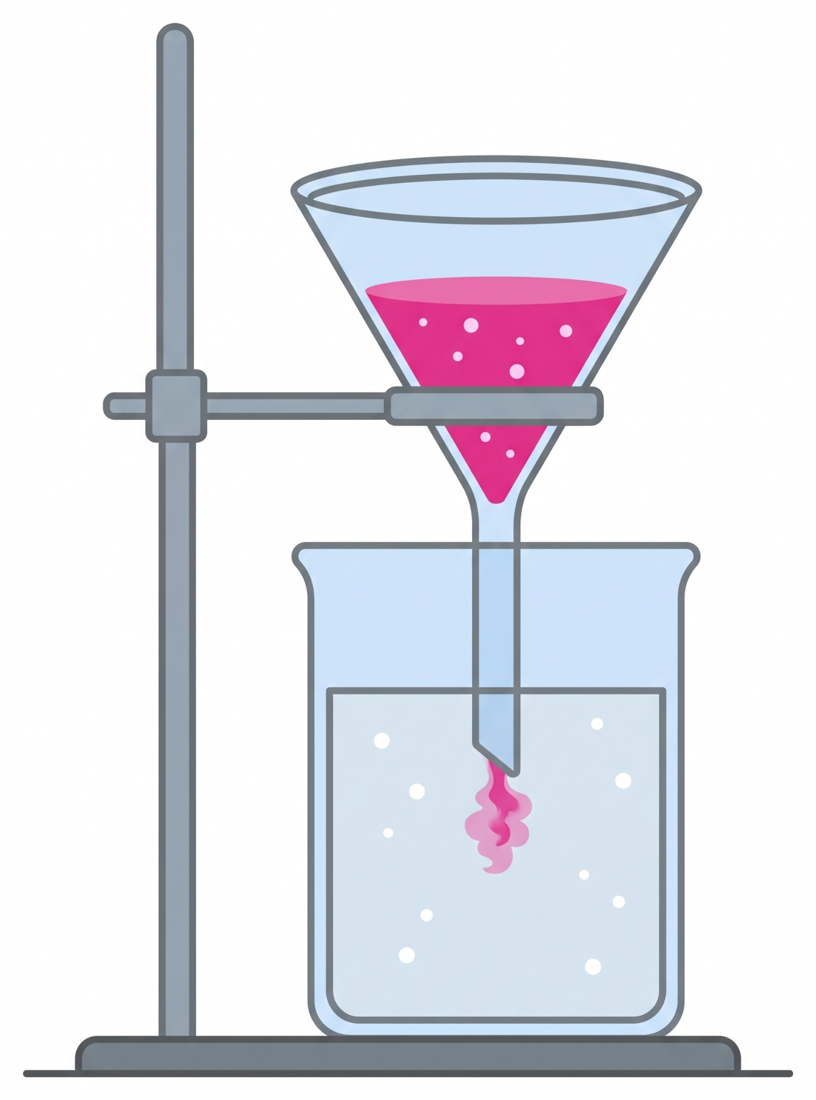
\includegraphics[width=0.86\linewidth]{rasmlar/darslik/d_nh3_fontan.png}\end{center}

\noindent A)~\textsl{1,67} \hfill B)~\textsl{1,7} \hfill C)~\textsl{3,34} \hfill D)~\textsl{0,84}\par
\qsep
\noindent\qn{32.} Kimyo laboratoriyasida ishlash qoidalari haqida qaysi fikrlar to`g`ri? 1) Konsentrlangan kislotani suvga ohista, aralashtirib quyiladi; 2) Kuygan joy ko`p suv bilan yuviladi; 3) Spirt lampa boshqa lampadan yoqilmaydi; 4) Zaharli gaz ajraladigan tajriba mo`rili shkafda o`tkaziladi

\noindent\begin{tabular}{@{}p{0.47\linewidth}@{}p{0.47\linewidth}@{}}
A)~\textsl{1, 2, 4} & B)~\textsl{2, 3, 4} \\
C)~\textsl{1, 2, 3} & D)~\textsl{1, 2, 3, 4   ---} \\
\end{tabular}\par
\qsep
\end{multicols}
\medskip
\noindent\setlength{\fboxsep}{0pt}\fbox{\begin{tabular}{p{0.74\linewidth}|p{0.2\linewidth}}
\parbox[t]{0.72\linewidth}{\vspace{3pt}\textbf{Topshiriqlar (33--35) va javob variant (A--F)larini o`zaro to`g`ri moslashtiring.} CuO va Fe\textsubscript{2}O\textsubscript{3} dan iborat 12 g aralashma qizdirilib, CO oqimida to`liq qaytarildi; qoldiq (metallar) massasi 8,8 g.
\vspace{3pt}} & \parbox[t]{0.19\linewidth}{\vspace{3pt}A~\textsl{2}\\[3pt]
B~\textsl{8,8}\\[3pt]
C~\textsl{8,06}\\[3pt]
D~\textsl{5,38}\\[3pt]
E~\textsl{4}\\[3pt]
F~\textsl{3,2}}\\ \hline
\parbox[t]{0.72\linewidth}{\vspace{2pt}\textbf{33. Aralashmadagi CuO massasini (g) aniqlang.}\vspace{2pt}} & \\ \hline
\parbox[t]{0.72\linewidth}{\vspace{2pt}\textbf{34. Qaytarish uchun (20\% ortiqcha olingan) sarflangan CO hajmini (l, n.sh.) aniqlang.}\vspace{2pt}} & \\ \hline
\parbox[t]{0.72\linewidth}{\vspace{2pt}\textbf{35. Qaytarish natijasida hosil bo`lgan CO\textsubscript{2} massasini (g) aniqlang.}\vspace{2pt}} & 
\end{tabular}}
\par\bigskip
\noindent\qn{36.} Fe + H\textsubscript{2}SO\textsubscript{4} $\to$ Fe\textsubscript{2}(SO\textsubscript{4})\textsubscript{3} + SO\textsubscript{2} + H\textsubscript{2}O reaksiya tenglamasini tenglang. Reagentlar (chap qism) koeffitsiyentlari \textbf{yig`indisini toping.}
\javob\qsep
\noindent\qn{37.} 4 l hajmli yopiq idishda 1 mol N\textsubscript{2}O\textsubscript{4} qizdirilganda N\textsubscript{2}O\textsubscript{4} $\rightleftarrows$ 2NO\textsubscript{2} muvozanati qaror topdi. Muvozanat aralashmasining vodorodga nisbatan zichligi 38,33 ga teng. Shu haroratdagi muvozanat \textbf{konstantasini (K, mol/l) hisoblang.}
\javob\qsep
\noindent\qn{38.} CaCO\textsubscript{3} va MgCO\textsubscript{3} dan iborat 18,4 g aralashma doimiy massagacha qizdirilganda qoldiq massasi 9,6 g bo`ldi. Aralashmadagi CaCO\textsubscript{3} ning \textbf{massasini (g) toping.}
\javob\qsep
\noindent\qn{39.} CH\textsubscript{3}OH va C\textsubscript{2}H\textsubscript{5}OH dan iborat 15,6 g aralashma natriy bilan to`liq reaksiyaga kirishganda ajraladigan vodorod \textbf{hajmini (l, n.sh.) toping.}
\javob\qsep
\noindent\qn{40.} 5,2 g asetilendan Kucherov reaksiyasi bilan (80\% unum) sirka aldegid olindi. Aldegid \textbf{massasini (g) aniqlang.}
\javob\qsep
\par\bigskip\begin{center}\textbf{\fontsize{13}{15}\selectfont YOZMA ISH}\end{center}
\noindent\qn{41.} \textbf{Topshiriqni bajarish jarayonida barcha reaksiya tenglamalarini yozing. Miqdoriy va arifmetik hisoblashlarni (unga asos bo`lgan usul yoki formulani ko`rsatgan holda) uzviy ketma-ketlikda bajaring.}\par\smallskip
Quyidagi eritmalar berilgan: HCl ning 0,02 mol/l li eritmasi va KOH ning 0,04 mol/l li eritmasi. Ularni aralashtirib, umumiy hajmi 1 l bo`lgan eritma tayyorlandi (0,5 l HCl eritmasi va 0,5 l KOH eritmasi). Shuningdek, sirka kislotaning 0,05 mol/l li eritmasida dissotsilanish darajasi 1\%.\par
\noindent 1)\ Aralashtirilgandan keyingi eritmaning pH ini aniqlang.\par
\noindent 2)\ Dastlabki HCl eritmasining pH ini hisoblang. 1 l shu eritmadagi HCl massasini (g) ham hisoblang.\par
\noindent 3)\ Dastlabki KOH eritmasining pH ini hisoblang.\par
\noindent 4)\ Sirka kislota eritmasidagi H\textsuperscript{+} ionlari konsentratsiyasini (mol/l) va pH ni aniqlang (lg 2 = 0,3, lg 5 = 0,7 ni ishlating). Shuningdek KOH eritmasi 100 marta suyultirilsa pH qancha bo`ladi?\par
\noindent 5)\ Sirka kislotaning dissotsilanish konstantasini hisoblang (K = C$\alpha$\textsuperscript{2}/(1 $-$ $\alpha$)). Shuningdek HCl eritmasi 10 marta suyultirilsa pH necha bo`ladi?\par
\diqqat{Mazkur topshiriq kengaytirilgan javobni talab etib, uning yechilish usuli va shu usul asosidagi barcha hisoblash amallari javoblar varaqasida aks etishi lozim.}\qsep
\noindent\qn{42.} Reaksiya tenglamalarini tugallang va tenglang. Hosil bo`lgan organik moddalarning tuzilish formulalarini yozing va ularni nomlang.\par
\noindent 1)\ 3C\textsubscript{2}H\textsubscript{2} $\xrightarrow{\text{C, t}}$\par
\noindent 2)\ CH\textsubscript{3}COONa + NaOH $\xrightarrow{\text{t}}$\par
\noindent 3)\ CH\textsubscript{2}=CH\textsubscript{2} + Br\textsubscript{2} $\to$\par
\noindent 4)\ CH\textsubscript{3}--C$\equiv$CH + H\textsubscript{2}O $\xrightarrow{\text{Hg\textsuperscript{2+}}}$\par
\noindent 5)\ CH\textsubscript{3}COOH + NaHCO\textsubscript{3} $\to$\par
\noindent 6)\ CH\textsubscript{3}--CH=CH\textsubscript{2} + HBr $\to$\par
\noindent 7)\ n CH\textsubscript{2}=CH--CH=CH\textsubscript{2} $\to$\par
\diqqat{Mazkur topshiriq kengaytirilgan javobni talab etib, uning yechilish usuli va shu usul asosidagi barcha hisoblash amallari javoblar varaqasida aks etishi lozim.}\qsep
\noindent\qn{43.} \textbf{Topshiriqni bajarish jarayonida barcha reaksiya tenglamalarini yozing. Miqdoriy va arifmetik hisoblashlarni (unga asos bo`lgan usul yoki formulani ko`rsatgan holda) uzviy ketma-ketlikda bajaring.}\par\smallskip
Temir (Fe) va rux (Zn) dan iborat 30,7 g qotishma mo`l suyultirilgan sulfat kislotada eritildi, bunda 11,2 l (n.sh.) gaz ajraldi. Hosil bo`lgan eritmaga mo`l NaOH eritmasi qo`shildi, hosil bo`lgan cho`kma ajratib olindi va havoda qizdirib quritildi.\par
\noindent 1)\ Reaksiya tenglamalarini yozing va qotishmadagi har bir metallning massasini (g) aniqlang.\par
\noindent 2)\ Qotishmadagi Fe ning massa ulushini (\%) hisoblang.\par
\noindent 3)\ Eritish uchun sarflangan 20\% li H\textsubscript{2}SO\textsubscript{4} eritmasining massasini (g) aniqlang.\par
\noindent 4)\ Mo`l NaOH qo`shilganda hosil bo`lgan cho`kmaning formulasi va massasini (g) toping (reaksiya tenglamalarini yozing).\par
\noindent 5)\ Cho`kma havoda to`liq qizdirilganda hosil bo`lgan oksidning massasini (g) hisoblang.\par
\diqqat{Mazkur topshiriq kengaytirilgan javobni talab etib, uning yechilish usuli va shu usul asosidagi barcha hisoblash amallari javoblar varaqasida aks etishi lozim.}\qsep
\newpage
\renewcommand{\curvar}{19-variant}
\thispagestyle{first}
\noindent\textit{Davriy jadvaldan foydalanish mumkin.}
\par\smallskip
\begin{multicols}{2}
\noindent\qn{1.} AgNO\textsubscript{3} eritmasi inert elektrodlar yordamida 4 A tok kuchi bilan 965 s elektroliz qilindi. Anodda ajralgan O\textsubscript{2} hajmi (l, n.sh.) \textbf{ni toping.}

\noindent A)~\textsl{0,448} \hfill B)~\textsl{0,112} \hfill C)~\textsl{0,009} \hfill D)~\textsl{0,224}\par
\qsep
\noindent\qn{2.} Xrom atomida d-pog`onachadagi elektronlar \textbf{sonini aniqlang} (\textit{Z} = 24).

\noindent A)~\textsl{5} \hfill B)~\textsl{6} \hfill C)~\textsl{4} \hfill D)~\textsl{7}\par
\qsep
\noindent\qn{3.} Mishyak (\textit{Z} = 33) atomining tashqi energetik pog`onasidagi elektronlar \textbf{sonini aniqlang.}

\noindent A)~\textsl{5} \hfill B)~\textsl{6} \hfill C)~\textsl{4} \hfill D)~\textsl{7}\par
\qsep
\noindent\qn{4.} Quyidagi tuzlarning qaysilari suvli eritmasi ishqoriy muhitga ega? 1) CH\textsubscript{3}COONa; 2) FeCl\textsubscript{3}; 3) K\textsubscript{2}S; 4) NH\textsubscript{4}Cl

\noindent A)~\textsl{2, 3, 4} \hfill B)~\textsl{1, 3} \hfill C)~\textsl{2, 3} \hfill D)~\textsl{3}\par
\qsep
\noindent\qn{5.} 2 mol Ba(OH)\textsubscript{2} va 2 mol NaCl suvda eritilib, eritma hajmi 4 l ga yetkazildi. Eritmadagi barcha ionlarning umumiy molyar \textbf{konsentratsiyasini (mol/l) aniqlang} (kuchli elektrolitlar to`liq dissotsilanadi).

\noindent A)~\textsl{1} \hfill B)~\textsl{5} \hfill C)~\textsl{2,5} \hfill D)~\textsl{1,25}\par
\qsep
\noindent\qn{6.} Kislotada Mg bo`lagi eritilganda ajralgan vodorod hajmining vaqtga bog`liqligi grafikda berilgan.
\begin{center}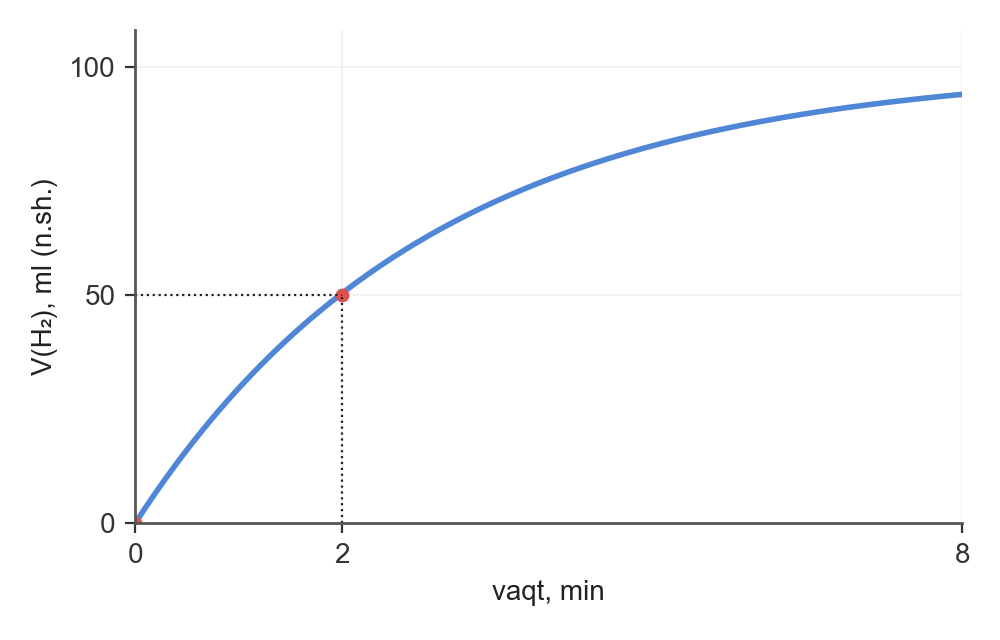
\includegraphics[width=0.86\linewidth]{rasmlar/gen/gv_v19_0.png}\end{center}
2-minutda ajralgan vodorodning \textbf{miqdorini (mmol) toping} (1 mmol gaz = 22,4 ml).

\noindent A)~\textsl{2,23} \hfill B)~\textsl{4,46} \hfill C)~\textsl{1,12} \hfill D)~\textsl{50}\par
\qsep
\noindent\qn{7.} Laboratoriyada CuSO\textsubscript{4} eritmalari quyidagicha tayyorlangan:
\begin{center}
\renewcommand{\arraystretch}{1.15}
\fitbox{\begin{tabular}{|c|c|c|}\hline
\textbf{Idish} & \textbf{Eritma massasi, g} & \textbf{$\omega$(CuSO\textsubscript{4}), \%} \\ \hline
A & 200 & 5 \\ \hline
B & 150 & 40 \\ \hline
\end{tabular}}
\end{center}
Bu ikki eritma bir idishga quyilib, yangi eritmadagi CuSO\textsubscript{4} ning massa ulushi (\%) qancha bo`ladi?

\noindent A)~\textsl{22,5} \hfill B)~\textsl{45} \hfill C)~\textsl{20} \hfill D)~\textsl{25}\par
\qsep
\noindent\qn{8.} Jadvalda bog`lar hosil qiluvchi atomlarning elektrmanfiyliklari berilgan:
\begin{center}
\renewcommand{\arraystretch}{1.15}
\fitbox{\begin{tabular}{|c|c|c|}\hline
\textbf{Bog`} & \textbf{EM (1-atom)} & \textbf{EM (2-atom)} \\ \hline
H--N & 2,1 & 3 \\ \hline
Mg--O & 1,2 & 3,5 \\ \hline
C--H & 2,5 & 2,1 \\ \hline
Si--O & 1,8 & 3,5 \\ \hline
\end{tabular}}
\end{center}
Qaysi bog` eng qutbli (eng ko`p ionli xarakterga ega)?

\noindent A)~\textsl{H--N} \hfill B)~\textsl{C--H} \hfill C)~\textsl{Si--O} \hfill D)~\textsl{Mg--O}\par
\qsep
\noindent\qn{9.} 8 g NaOH va 5,48 g HCl aralashtirilib, reaksiya o`tkazildi (NaOH + HCl $\to$ NaCl + H\textsubscript{2}O). Hosil bo`lgan NaCl \textbf{massasini (g) aniqlang.}

\noindent A)~\textsl{11,7} \hfill B)~\textsl{17,55} \hfill C)~\textsl{4,39} \hfill D)~\textsl{8,78}\par
\qsep
\noindent\qn{10.} 131,2 l N\textsubscript{2} 127 \textdegree{}C va 0,5 atm bosimda necha gramm keladi? (R = 0,082 l$\cdot$atm/(mol$\cdot$K))

\noindent A)~\textsl{112} \hfill B)~\textsl{56} \hfill C)~\textsl{28} \hfill D)~\textsl{164}\par
\qsep
\noindent\qn{11.} HC$\equiv$C--CH=CH\textsubscript{2} molekulasidagi $\sigma$ va $\pi$ bog`lar \textbf{sonini aniqlang.}

\noindent A)~\textsl{6 va 3} \hfill B)~\textsl{7 va 4} \hfill C)~\textsl{8 va 3} \hfill D)~\textsl{7 va 3}\par
\qsep
\noindent\qn{12.} K\textsubscript{2}Cr\textsubscript{2}O\textsubscript{7} tarkibida Cr ning oksidlanish \textbf{darajasini aniqlang.}

\noindent A)~\textsl{$-$1} \hfill B)~\textsl{+1} \hfill C)~\textsl{+6} \hfill D)~\textsl{$-$3}\par
\qsep
\noindent\qn{13.} Faqat qaytaruvchi bo`la oladigan \textbf{ionlarni aniqlang}: 1) Al\textsuperscript{3+}; 2) S\textsuperscript{2$-$}; 3) Na\textsuperscript{+}; 4) Fe\textsuperscript{3+}

\noindent A)~\textsl{1, 4} \hfill B)~\textsl{1, 3} \hfill C)~\textsl{3, 4} \hfill D)~\textsl{2}\par
\qsep
\noindent\qn{14.} Reaksiya tenglamasi: SiO\textsubscript{2} + 2NaOH $\to$ Na\textsubscript{2}SiO\textsubscript{3} + H\textsubscript{2}O. Reaksiyaga tarkibida 20\% aralashma bo`lgan 20 g namuna (asosiy modda NaOH) kirishdi. Na\textsubscript{2}SiO\textsubscript{3} \textbf{massasini (g) hisoblang.}

\noindent A)~\textsl{97,6} \hfill B)~\textsl{48,8} \hfill C)~\textsl{24,4} \hfill D)~\textsl{12,2}\par
\qsep
\noindent\qn{15.} 2NaBr + Cl\textsubscript{2} $\to$ 2NaCl + Br\textsubscript{2} reaksiyasida 71 g Cl\textsubscript{2} ishtirok etdi. Br\textsubscript{2} \textbf{miqdorini (mol) toping.}

\noindent A)~\textsl{1} \hfill B)~\textsl{2} \hfill C)~\textsl{0,5} \hfill D)~\textsl{1,5}\par
\qsep
\noindent\qn{16.} Ishqoriy metallar haqida qaysi fikrlar to`g`ri? 1) KOH -- kuchli ishqor; 2) Natriy atomining tashqi qavatida 2 ta elektron bor; 3) Natriy kerosin ostida saqlanadi; 4) Natriy suv bilan reaksiyada H\textsubscript{2} va NaOH hosil qiladi

\noindent A)~\textsl{1, 2, 3} \hfill B)~\textsl{1, 3, 4} \hfill C)~\textsl{2, 3} \hfill D)~\textsl{1, 2, 4}\par
\qsep
\noindent\qn{17.} Mg\textsubscript{3}N\textsubscript{2} + 6H\textsubscript{2}O $\to$ 3Mg(OH)\textsubscript{2} + 2NH\textsubscript{3} jarayoni uchun 50 g Mg\textsubscript{3}N\textsubscript{2} olingan (unum 90\%). NH\textsubscript{3} \textbf{hajmini (l, n.sh.) aniqlang.}

\noindent A)~\textsl{5,6} \hfill B)~\textsl{40,32} \hfill C)~\textsl{20,16} \hfill D)~\textsl{10,08}\par
\qsep
\noindent\qn{18.} 4,5 g Fe(OH)\textsubscript{2} havoda to`liq oksidlanib, Fe(OH)\textsubscript{3} ga aylandi. Hosil bo`lgan Fe(OH)\textsubscript{3} \textbf{massasini (g) aniqlang.}

\noindent A)~\textsl{4,5} \hfill B)~\textsl{5,35} \hfill C)~\textsl{8,03} \hfill D)~\textsl{4,95}\par
\qsep
\noindent\qn{19.} Ca(HCO\textsubscript{3})\textsubscript{2} + Ca(OH)\textsubscript{2} $\to$ 2CaCO\textsubscript{3} + 2H\textsubscript{2}O reaksiyasida 40,5 g Ca(HCO\textsubscript{3})\textsubscript{2} ishtirok etdi (unum 50\%). CaCO\textsubscript{3} \textbf{massasini (g) toping.}

\noindent A)~\textsl{12,5} \hfill B)~\textsl{50} \hfill C)~\textsl{25} \hfill D)~\textsl{37,5}\par
\qsep
\noindent\qn{20.} C\textsubscript{4}H\textsubscript{6} alkinlarning izomerlari soni nechta?

\noindent A)~\textsl{3} \hfill B)~\textsl{1} \hfill C)~\textsl{4} \hfill D)~\textsl{2}\par
\qsep
\noindent\qn{21.} CH\textsubscript{2}=CH--CH=CH\textsubscript{2} birikmaning sistematik nomi qaysi qatorda to`g`ri keltirilgan?

\noindent\begin{tabular}{@{}p{0.47\linewidth}@{}p{0.47\linewidth}@{}}
A)~\textsl{butadiyen-1,3} & B)~\textsl{butadiyen-1,2} \\
C)~\textsl{buten-1} & D)~\textsl{butin-1} \\
\end{tabular}\par
\qsep
\noindent\qn{22.} C\textsubscript{6}H\textsubscript{6} + HNO\textsubscript{3} $\to$ C\textsubscript{6}H\textsubscript{5}NO\textsubscript{2} + H\textsubscript{2}O reaksiyasida 156 g C\textsubscript{6}H\textsubscript{6} ishtirok etdi. HNO\textsubscript{3} \textbf{massasini (g) toping.}

\noindent A)~\textsl{252} \hfill B)~\textsl{63} \hfill C)~\textsl{126} \hfill D)~\textsl{189}\par
\qsep
\noindent\qn{23.} Spirt va fenollar haqida qaysi fikrlar to`g`ri? 1) Etilenglikol zaharsiz; 2) Etanol natriy bilan reaksiyaga kirishadi; 3) Glitserin Cu(OH)\textsubscript{2} bilan ko`k kompleks hosil qiladi; 4) Fenol Cu(OH)\textsubscript{2} ni eritib ko`k kompleks hosil qiladi

\noindent A)~\textsl{2, 3} \hfill B)~\textsl{4} \hfill C)~\textsl{3, 4} \hfill D)~\textsl{2, 4}\par
\qsep
\noindent\qn{24.} Aldegid va ketonlar haqida qaysi fikrlar to`g`ri? 1) Formalin --- formaldegidning 40\% li eritmasi; 2) Ketonlar kuchsiz oksidlovchilar bilan oksidlanmaydi; 3) Aldegidlar qaytarilganda ikkilamchi spirt hosil bo`ladi; 4) Aldegidlar "kumush ko`zgu" reaksiyasini beradi

\noindent A)~\textsl{2, 3} \hfill B)~\textsl{1, 3} \hfill C)~\textsl{1, 3, 4} \hfill D)~\textsl{1, 2, 4}\par
\qsep
\noindent\qn{25.} C\textsubscript{4}H\textsubscript{8} alkenlarning izomerlari soni (sis-trans izomerlar bilan, siklik bo`lmagan) nechta?

\noindent A)~\textsl{5} \hfill B)~\textsl{3} \hfill C)~\textsl{6} \hfill D)~\textsl{4}\par
\qsep
\noindent\qn{26.} CH\textsubscript{3}COOH + C\textsubscript{2}H\textsubscript{5}OH $\to$ CH\textsubscript{3}COOC\textsubscript{2}H\textsubscript{5} + H\textsubscript{2}O reaksiyasida 120 g CH\textsubscript{3}COOH ishtirok etdi. CH\textsubscript{3}COOC\textsubscript{2}H\textsubscript{5} \textbf{massasini (g) toping.}

\noindent A)~\textsl{176} \hfill B)~\textsl{352} \hfill C)~\textsl{88} \hfill D)~\textsl{264}\par
\qsep
\noindent\qn{27.} Uglevodlar haqida qaysi fikrlar to`g`ri? 1) Kraxmal va selluloza bir xil M ga ega; 2) Kraxmal yod bilan ko`k rang beradi; 3) Saxaroza Feling suyuqligini qaytaradi; 4) Fruktoza ketospirt

\noindent A)~\textsl{2, 4} \hfill B)~\textsl{2} \hfill C)~\textsl{1, 2} \hfill D)~\textsl{1, 3, 4}\par
\qsep
\noindent\qn{28.} Rasmda benzol hosilasining tuzilish formulasi berilgan.
\begin{center}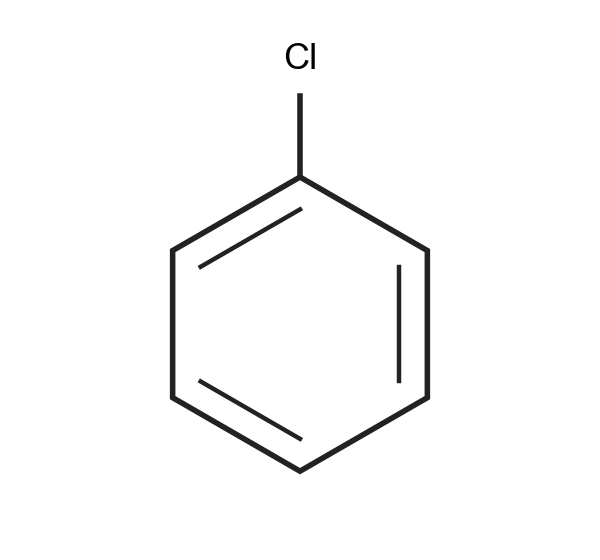
\includegraphics[width=0.86\linewidth]{rasmlar/gen/bs_14476.png}\end{center}
Birikmaning molekulyar \textbf{formulasini aniqlang.}

\noindent A)~\textsl{C\textsubscript{7}H\textsubscript{6}O\textsubscript{2}} \hfill B)~\textsl{C\textsubscript{6}H\textsubscript{5}NO\textsubscript{2}} \hfill C)~\textsl{C\textsubscript{6}H\textsubscript{5}Cl} \hfill D)~\textsl{C\textsubscript{6}H\textsubscript{6}O}\par
\qsep
\noindent\qn{29.} Reaksiya tenglamasi: C\textsubscript{2}H\textsubscript{2} + HCl $\to$ C\textsubscript{2}H\textsubscript{3}Cl. Reaksiyaga 5,2 g C\textsubscript{2}H\textsubscript{2} kirishdi. C\textsubscript{2}H\textsubscript{3}Cl \textbf{miqdorini (mol) hisoblang.}

\noindent A)~\textsl{0,4} \hfill B)~\textsl{0,2} \hfill C)~\textsl{0,1} \hfill D)~\textsl{0,3}\par
\qsep
\noindent\qn{30.} Eritmaga NaOH qo`shilganda havorang cho`kma (Cu(OH)\textsubscript{2}) kuzatildi. Eritmada qaysi ion bor?

\noindent A)~\textsl{PO\textsubscript{4}\textsuperscript{3$-$}} \hfill B)~\textsl{Cu\textsuperscript{2+}} \hfill C)~\textsl{Cl\textsuperscript{$-$}} \hfill D)~\textsl{Fe\textsuperscript{3+}}\par
\qsep
\noindent\qn{31.} Lakmus indikatori neytral muhitda qanday rang beradi?
\noindent A)~\textsl{ko`k}\par
\noindent B)~\textsl{binafsha}\par
\noindent C)~\textsl{malina rangga kiradi (pushti)}\par
\noindent D)~\textsl{qizil}\par
\qsep
\noindent\qn{32.} Rasmdagi asbobda 23 g etanol konsentrlangan H\textsubscript{2}SO\textsubscript{4} bilan 170 \textdegree{}C da qizdirilib, 90\% unum bilan etilen olindi. Hosil bo`lgan etilen \textbf{hajmini (l, n.sh.) aniqlang.}
\begin{center}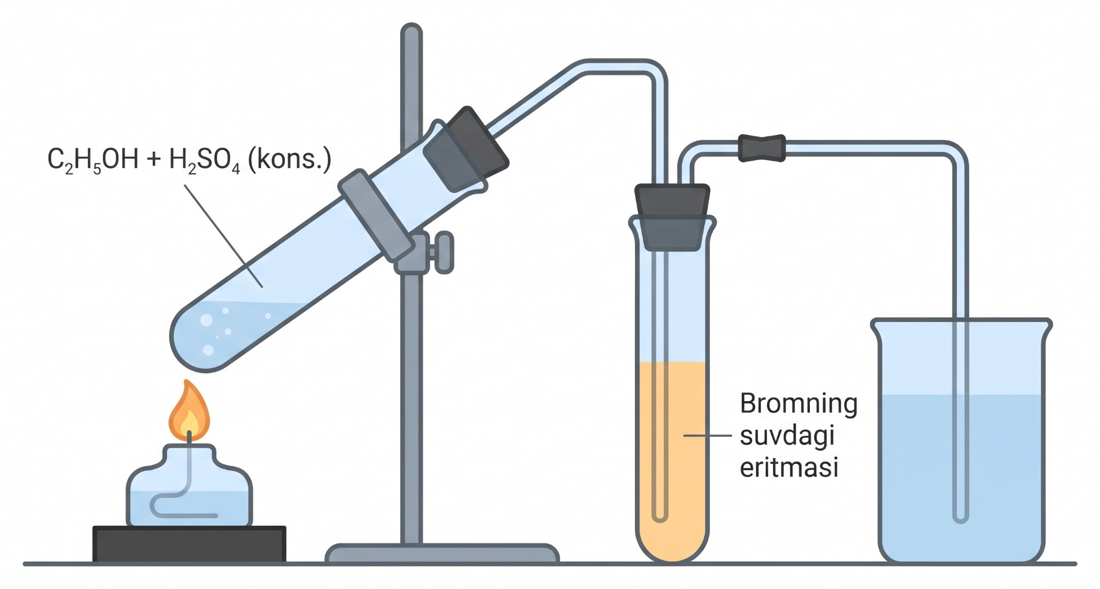
\includegraphics[width=0.86\linewidth]{rasmlar/darslik/d_etilen.png}\end{center}

\noindent\begin{tabular}{@{}p{0.47\linewidth}@{}p{0.47\linewidth}@{}}
A)~\textsl{11,2} & B)~\textsl{10,08} \\
C)~\textsl{20,16} & D)~\textsl{5,04   ---} \\
\end{tabular}\par
\qsep
\end{multicols}
\medskip
\noindent\setlength{\fboxsep}{0pt}\fbox{\begin{tabular}{p{0.74\linewidth}|p{0.2\linewidth}}
\parbox[t]{0.72\linewidth}{\vspace{3pt}\textbf{Topshiriqlar (33--35) va javob variant (A--F)larini o`zaro to`g`ri moslashtiring.} Rux va temir (Zn va Fe) dan iborat 20,05 g qotishma mo`l HCl eritmasida eritilganda 7,84 l (n.sh.) gaz ajraldi.
\vspace{3pt}} & \parbox[t]{0.19\linewidth}{\vspace{3pt}A~\textsl{67,35}\\[3pt]
B~\textsl{35,92}\\[3pt]
C~\textsl{24,31}\\[3pt]
D~\textsl{127,75}\\[3pt]
E~\textsl{44,9}\\[3pt]
F~\textsl{16,21}}\\ \hline
\parbox[t]{0.72\linewidth}{\vspace{2pt}\textbf{33. Qotishmadagi Zn massa ulushini (\%) aniqlang.}\vspace{2pt}} & \\ \hline
\parbox[t]{0.72\linewidth}{\vspace{2pt}\textbf{34. Reaksiya uchun sarflangan 20\% li HCl massasini (g) aniqlang.}\vspace{2pt}} & \\ \hline
\parbox[t]{0.72\linewidth}{\vspace{2pt}\textbf{35. Eritmadagi tuzlarning umumiy massasini (g) aniqlang.}\vspace{2pt}} & 
\end{tabular}}
\par\bigskip
\noindent\qn{36.} H\textsubscript{2}S + HNO\textsubscript{3} $\to$ H\textsubscript{2}SO\textsubscript{4} + NO\textsubscript{2} + H\textsubscript{2}O reaksiya tenglamasini elektron balans usulida tenglang va barcha koeffitsiyentlar \textbf{yig`indisini aniqlang.}
\javob\qsep
\noindent\qn{37.} CH\textsubscript{4} va H\textsubscript{2} dan iborat 60 ml aralashma mo`l kisloroda yondirildi (suv suyuq holatda; hajmlar bir xil sharoitda o`lchandi). Reaksiyadan so`ng gazlar hajmi 105 ml ga kamaydi. Aralashmadagi CH\textsubscript{4} \textbf{hajmini (ml) toping.}
\javob\qsep
\noindent\qn{38.} Al, Fe va Cu dan iborat aralashma mo`l NaOH eritmasi bilan ta'sirlashganda 6,72 l (n.sh.) vodorod ajraldi; xuddi shunday massadagi aralashma mo`l HCl bilan ta'sirlashganda 11,2 l (n.sh.) vodorod ajraldi, erimay qolgan qoldiq (mis) massasi 6,4 g. Aralashmaning dastlabki \textbf{massasini (g) toping.}
\javob\qsep
\noindent\qn{39.} 23 g etanol avval sirka aldegidgacha (unum 90\%), so`ng sirka kislotagacha (unum 80\%) oksidlandi; hosil bo`lgan kislota mo`l etanol bilan efirlandi (unum 100\%). Etilatsetat \textbf{massasini (g) toping.}
\javob\qsep
\noindent\qn{40.} 18 g sirka kislota va 9,2 g etanol dan 80\% unum bilan murakkab efir olindi. Efir \textbf{massasini (g) toping.}
\javob\qsep
\par\bigskip\begin{center}\textbf{\fontsize{13}{15}\selectfont YOZMA ISH}\end{center}
\noindent\qn{41.} \textbf{Topshiriqni bajarish jarayonida barcha reaksiya tenglamalarini yozing. Miqdoriy va arifmetik hisoblashlarni (unga asos bo`lgan usul yoki formulani ko`rsatgan holda) uzviy ketma-ketlikda bajaring.}\par\smallskip
12,5 g CuSO\textsubscript{4}$\cdot$5H\textsubscript{2}O 400 g suvda eritildi.\par
\noindent 1)\ Hosil bo`lgan eritmadagi CuSO\textsubscript{4} ning massa ulushini (\%) toping.\par
\noindent 2)\ Eritmaga mo`l BaCl\textsubscript{2} eritmasi qo`shildi. Hosil bo`lgan cho`kma massasini (g) toping. Eritmadagi kation miqdorini (mol) ham toping.\par
\noindent 3)\ Xuddi shunday eritmaga ekvivalent miqdorda NaOH qo`shilganda hosil bo`lgan Cu(OH)\textsubscript{2} cho`kmasining massasini (g) toping.\par
\noindent 4)\ Eritmaga Fe plastinka tushirildi (CuSO\textsubscript{4} tuzidagi metall to`liq siqib chiqarildi). Plastinka massasi qanchaga (g) o`zgargan? Dastlabki eritma massasini (g) ham ayting.\par
\noindent 5)\ Kristallogidratdagi kristallizatsion suvning massa ulushini (\%) va unda suv molekulalari sonini toping. Shu miqdor kristallogidrat suvsizlantirilganda massa necha gramm kamayadi?\par
\diqqat{Mazkur topshiriq kengaytirilgan javobni talab etib, uning yechilish usuli va shu usul asosidagi barcha hisoblash amallari javoblar varaqasida aks etishi lozim.}\qsep
\noindent\qn{42.} Quyidagi o`zgarishlar zanjirida \textit{X}, \textit{Y}, \textit{Z} noma'lum organik moddalar:\par
\[\setlength{\fboxsep}{0pt}\text{C\textsubscript{2}H\textsubscript{4}Br\textsubscript{2}}\xrightarrow{\text{KOH (spirtli)}}\text{\textit{X}}\xrightarrow{\text{C (aktiv), 600 \textdegree{}C}}\text{\textit{Y}}\xrightarrow{\text{HNO\textsubscript{3}, H\textsubscript{2}SO\textsubscript{4}}}\text{C\textsubscript{6}H\textsubscript{5}NO\textsubscript{2}}\]
\noindent 1)\ C\textsubscript{2}H\textsubscript{4}Br\textsubscript{2} $\to$ \textit{X} : reaksiya tenglamasini yozing; hosil bo`lgan moddani nomlang.\par
\noindent 2)\ \textit{X} $\to$ \textit{Y} : reaksiya tenglamasini yozing; hosil bo`lgan moddani nomlang.\par
\noindent 3)\ \textit{Y} $\to$ C\textsubscript{6}H\textsubscript{5}NO\textsubscript{2} : reaksiya tenglamasini yozing; hosil bo`lgan moddani nomlang.\par
\diqqat{Mazkur topshiriq kengaytirilgan javobni talab etib, uning yechilish usuli va shu usul asosidagi barcha hisoblash amallari javoblar varaqasida aks etishi lozim.}\qsep
\noindent\qn{43.} \textbf{Topshiriqni bajarish jarayonida barcha reaksiya tenglamalarini yozing. Miqdoriy va arifmetik hisoblashlarni (unga asos bo`lgan usul yoki formulani ko`rsatgan holda) uzviy ketma-ketlikda bajaring.}\par\smallskip
Uch probirkada (\textit{X}, \textit{Y}, \textit{Z}) natriy yoki kaliy tuzlarining eritmalari bor: KI, Na\textsubscript{3}PO\textsubscript{4}, NaBr (tartibsiz). Har bir eritmaga reagentlar ta'sir ettirildi, kuzatuvlar jadvalda:\par
\begin{center}
\renewcommand{\arraystretch}{1.15}
\begin{tabular}{|c|c|c|c|}\hline
\textbf{Reagent} & \textbf{\textit{X}} & \textbf{\textit{Y}} & \textbf{\textit{Z}} \\ \hline
AgNO\textsubscript{3} & sariq cho`kma (AgI) & sariq cho`kma (Ag\textsubscript{3}PO\textsubscript{4}) & och sariq cho`kma (AgBr) \\ \hline
BaCl\textsubscript{2} & --- & oq cho`kma & --- \\ \hline
HCl & --- & --- & --- \\ \hline
\end{tabular}
\end{center}
\noindent 1)\ \textit{X}, \textit{Y}, \textit{Z} probirkalardagi moddalarni aniqlang va kuzatilgan reaksiyalarning ionli tenglamalarini yozing.\par
\noindent 2)\ \textit{Y} probirkadagi tuz 0,05 mol miqdorda olingan. Unga mo`l AgNO\textsubscript{3} qo`shilganda hosil bo`lgan cho`kma massasini (g) toping.\par
\noindent 3)\ Uchala eritmaning har biriga 0,05 mol dan solingan bo`lsa, mo`l AgNO\textsubscript{3} qo`shilganda hosil bo`ladigan barcha cho`kmalarning umumiy massasini (g) toping (ularning formulalarini yozing).\par
\noindent 4)\ Eritmalarda kuzatilgan hodisalarni (cho`kma yoki gaz hosil bo`lishi) tushuntiring: qaysi ion qaysi reagent bilan qanday birikma hosil qiladi? Shu usul bilan ionlarni aniqlash qoidasini yozing.\par
\noindent 5)\ Uchala eritmaning har biriga 0,05 mol dan solingan. AgNO\textsubscript{3} bilan cho`kadigan ionlarni to`liq cho`ktirish uchun 10\% li AgNO\textsubscript{3} eritmasidan necha gramm kerak?\par
\diqqat{Mazkur topshiriq kengaytirilgan javobni talab etib, uning yechilish usuli va shu usul asosidagi barcha hisoblash amallari javoblar varaqasida aks etishi lozim.}\qsep
\newpage
\renewcommand{\curvar}{20-variant}
\thispagestyle{first}
\noindent\textit{Davriy jadvaldan foydalanish mumkin.}
\par\smallskip
\begin{multicols}{2}
\noindent\qn{1.} 1 g He 127 \textdegree{}C va 1 atm bosimda qancha hajm (l) egallaydi? (R = 0,082 l$\cdot$atm/(mol$\cdot$K))

\noindent A)~\textsl{8,2} \hfill B)~\textsl{16,4} \hfill C)~\textsl{4,1} \hfill D)~\textsl{5,6}\par
\qsep
\noindent\qn{2.} Quyidagi tuzlarning qaysilari suvli eritmasi kislotali muhitga ega? 1) NH\textsubscript{4}Cl; 2) KNO\textsubscript{3}; 3) FeCl\textsubscript{3}; 4) Na\textsubscript{2}SO\textsubscript{4}

\noindent A)~\textsl{2} \hfill B)~\textsl{1, 2} \hfill C)~\textsl{2, 3, 4} \hfill D)~\textsl{1, 3}\par
\qsep
\noindent\qn{3.} Quyidagilarni jism va moddalarga ajrating: mix, qaychi, etanol, alyuminiy, kislorod, osh tuzi. Ulardan nechtasi modda?

\noindent A)~\textsl{4} \hfill B)~\textsl{5} \hfill C)~\textsl{3} \hfill D)~\textsl{2}\par
\qsep
\noindent\qn{4.} Jadvalda bog`lar hosil qiluvchi atomlarning elektrmanfiyliklari berilgan:
\begin{center}
\renewcommand{\arraystretch}{1.15}
\fitbox{\begin{tabular}{|c|c|c|}\hline
\textbf{Bog`} & \textbf{EM (1-atom)} & \textbf{EM (2-atom)} \\ \hline
Na--Cl & 0,9 & 3 \\ \hline
N--H & 3 & 2,1 \\ \hline
H--F & 2,1 & 4 \\ \hline
Mg--O & 1,2 & 3,5 \\ \hline
\end{tabular}}
\end{center}
Qaysi bog` eng qutbli (eng ko`p ionli xarakterga ega)?

\noindent A)~\textsl{Na--Cl} \hfill B)~\textsl{N--H} \hfill C)~\textsl{Mg--O} \hfill D)~\textsl{H--F}\par
\qsep
\noindent\qn{5.} 3 mol AlCl\textsubscript{3} va 2 mol HNO\textsubscript{3} suvda eritilib, eritma hajmi 5 l ga yetkazildi. Eritmadagi barcha ionlarning umumiy molyar \textbf{konsentratsiyasini (mol/l) aniqlang} (kuchli elektrolitlar to`liq dissotsilanadi).

\noindent A)~\textsl{1} \hfill B)~\textsl{6,4} \hfill C)~\textsl{3,2} \hfill D)~\textsl{1,6}\par
\qsep
\noindent\qn{6.} 2SO\textsubscript{2} + O\textsubscript{2} $\rightleftarrows$ 2SO\textsubscript{3} reaksiyasida SO\textsubscript{2} va O\textsubscript{2} stexiometrik nisbatda olingan umumiy 12 mol aralashma muvozanat qaror topganda doimiy T va \textit{V} da bosim 25\% ga kamaydi. Muvozanatdagi SO\textsubscript{3} ning \textbf{miqdorini (mol) aniqlang.}

\noindent A)~\textsl{2} \hfill B)~\textsl{1} \hfill C)~\textsl{6} \hfill D)~\textsl{3}\par
\qsep
\noindent\qn{7.} 1 mol C\textsubscript{2}H\textsubscript{6} tarkibida necha mol atom bor?

\noindent A)~\textsl{7} \hfill B)~\textsl{8} \hfill C)~\textsl{9} \hfill D)~\textsl{1}\par
\qsep
\noindent\qn{8.} Quyidagi zarrachalardan qaysilari neon atomi bilan izoelektron? 1) O\textsuperscript{2$-$}; 2) Mg\textsuperscript{2+}; 3) Ca\textsuperscript{2+}; 4) K\textsuperscript{+}

\noindent A)~\textsl{1, 2, 4} \hfill B)~\textsl{2, 3, 4} \hfill C)~\textsl{1, 2} \hfill D)~\textsl{1, 3}\par
\qsep
\noindent\qn{9.} Grafikda tuzning eruvchanligi (g/100 g suv) haroratga bog`liq ko`rsatilgan.
\begin{center}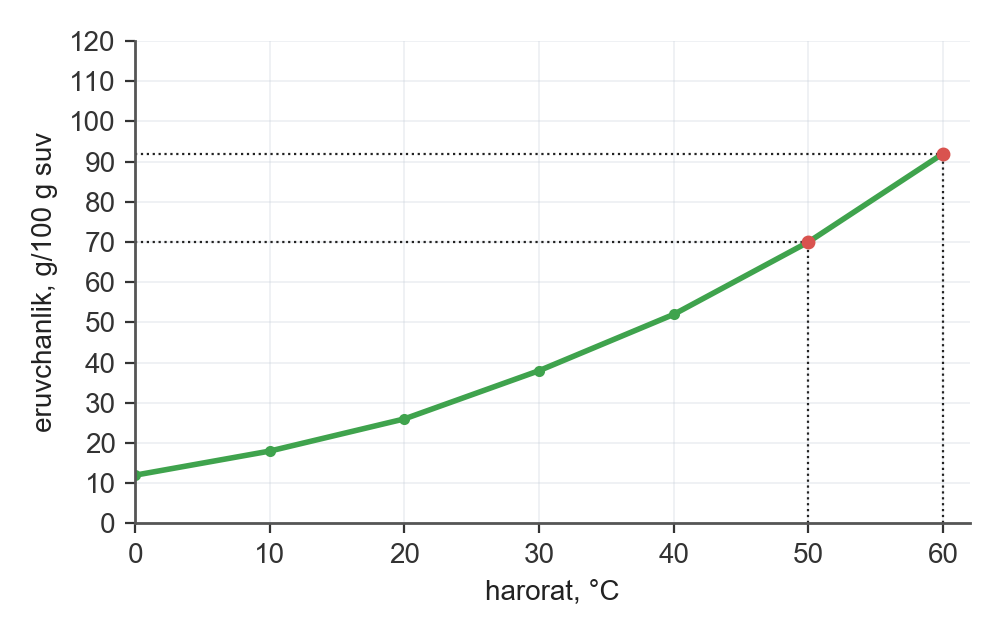
\includegraphics[width=0.86\linewidth]{rasmlar/gen/sol_v20_0.png}\end{center}
60 \textdegree{}C da tuzning to`yingan eritmasidagi massa \textbf{ulushini (\%) aniqlang.}

\noindent A)~\textsl{47,9} \hfill B)~\textsl{92} \hfill C)~\textsl{24} \hfill D)~\textsl{41,2}\par
\qsep
\noindent\qn{10.} Laboratoriyada KNO\textsubscript{3} eritmalari quyidagicha tayyorlangan:
\begin{center}
\renewcommand{\arraystretch}{1.15}
\fitbox{\begin{tabular}{|c|c|c|}\hline
\textbf{Idish} & \textbf{Eritma massasi, g} & \textbf{$\omega$(KNO\textsubscript{3}), \%} \\ \hline
A & 200 & 20 \\ \hline
B & 300 & 35 \\ \hline
\end{tabular}}
\end{center}
Bu ikki eritma bir idishga quyilib, yangi eritmadagi KNO\textsubscript{3} ning massa ulushi (\%) qancha bo`ladi?

\noindent A)~\textsl{27,5} \hfill B)~\textsl{55} \hfill C)~\textsl{26} \hfill D)~\textsl{29}\par
\qsep
\noindent\qn{11.} N\textsubscript{2} gazining 27 \textdegree{}C va 4 atm bosimdagi \textbf{zichligini (g/l) aniqlang.} (R = 0,082 l$\cdot$atm/(mol$\cdot$K))

\noindent A)~\textsl{9,11} \hfill B)~\textsl{4,55} \hfill C)~\textsl{2,28} \hfill D)~\textsl{1,25}\par
\qsep
\noindent\qn{12.} Rasmda davriy jadvalning bir qismi berilgan (\textit{X}, \textit{Y}, \textit{Z} --- noma'lum elementlar).
\begin{center}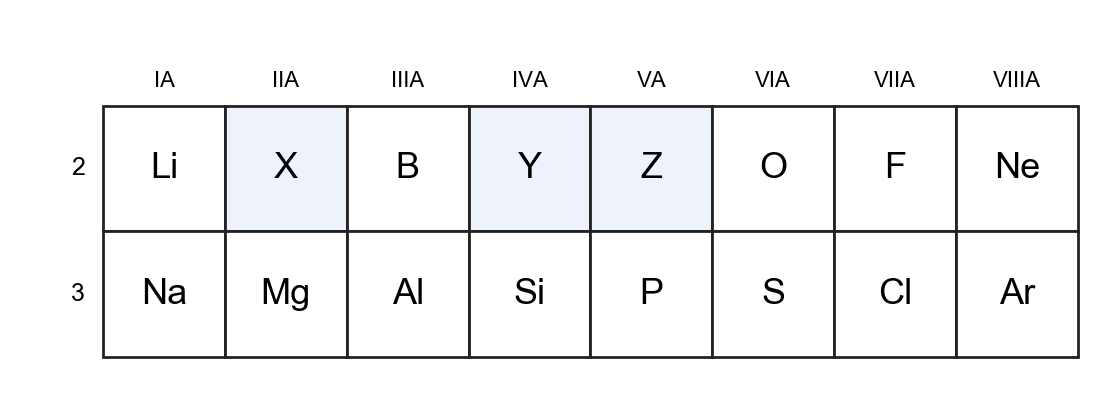
\includegraphics[width=0.86\linewidth]{rasmlar/gen/pt_580869.png}\end{center}
\textit{X}, \textit{Y}, \textit{Z} elementlardan qaysi birining elektrmanfiyligi eng katta?

\noindent\begin{tabular}{@{}p{0.47\linewidth}@{}p{0.47\linewidth}@{}}
A)~\textsl{\textit{X}} & B)~\textsl{\textit{Z}} \\
C)~\textsl{\textit{Y}} & D)~\textsl{uchalasiniki teng} \\
\end{tabular}\par
\qsep
\noindent\qn{13.} AgNO\textsubscript{3} ning suvli eritmasi inert elektrodlar bilan elektroliz qilinganda qaysi moddalar ajraladi?

\noindent\begin{tabular}{@{}p{0.47\linewidth}@{}p{0.47\linewidth}@{}}
A)~\textsl{Cu va Cl\textsubscript{2}} & B)~\textsl{Ag va O\textsubscript{2}} \\
C)~\textsl{H\textsubscript{2}, Cl\textsubscript{2} va NaOH} & D)~\textsl{Zn, H\textsubscript{2} va O\textsubscript{2}} \\
\end{tabular}\par
\qsep
\noindent\qn{14.} Ishqoriy metallar haqida qaysi fikrlar to`g`ri? 1) KOH -- kuchli ishqor; 2) Natriyning olinishi suyuqlanma NaCl elektrolizi bilan; 3) Natriy atomining tashqi qavatida 2 ta elektron bor; 4) Natriy suv bilan reaksiyada H\textsubscript{2} va NaOH hosil qiladi

\noindent A)~\textsl{1, 2, 4} \hfill B)~\textsl{2, 4} \hfill C)~\textsl{1, 2} \hfill D)~\textsl{2, 3}\par
\qsep
\noindent\qn{15.} Alyuminiy va mis dan iborat 14,5 g aralashma mo`l NaOH eritmasida eritilganda 10,08 l (n.sh.) gaz ajraldi. Aralashmadagi mis ning massa \textbf{ulushini (\%) aniqlang.}

\noindent A)~\textsl{55,9} \hfill B)~\textsl{44,1} \hfill C)~\textsl{22,1} \hfill D)~\textsl{50,3}\par
\qsep
\noindent\qn{16.} D-metallar va ularning birikmalari haqida qaysi fikrlar to`g`ri? 1) Temir sovuq konsentrlangan HNO\textsubscript{3} da passivlanadi; 2) Mis nam havoda (CuOH)\textsubscript{2}CO\textsubscript{3} qoplamasi bilan qoplanadi; 3) Cr\textsubscript{2}O\textsubscript{3} asosli oksid; 4) Zn(OH)\textsubscript{2} amfoter xossaga ega

\noindent A)~\textsl{1, 2, 4} \hfill B)~\textsl{3, 4} \hfill C)~\textsl{1, 2} \hfill D)~\textsl{2, 3}\par
\qsep
\noindent\qn{17.} Reaksiya tenglamasi: CaSO\textsubscript{4} + Na\textsubscript{2}CO\textsubscript{3} $\to$ CaCO\textsubscript{3} + Na\textsubscript{2}SO\textsubscript{4}. Reaksiyaga tarkibida 75\% aralashma bo`lgan 136 g namuna (asosiy modda CaSO\textsubscript{4}) kirishdi. Na\textsubscript{2}SO\textsubscript{4} \textbf{massasini (g) hisoblang.}

\noindent A)~\textsl{71} \hfill B)~\textsl{17,75} \hfill C)~\textsl{53,25} \hfill D)~\textsl{35,5}\par
\qsep
\noindent\qn{18.} Al\textsubscript{2}O\textsubscript{3} + 3H\textsubscript{2}SO\textsubscript{4} $\to$ Al\textsubscript{2}(SO\textsubscript{4})\textsubscript{3} + 3H\textsubscript{2}O jarayoni uchun 9,8 g H\textsubscript{2}SO\textsubscript{4} olingan. Al\textsubscript{2}O\textsubscript{3} \textbf{massasini (g) aniqlang.}

\noindent A)~\textsl{30,6} \hfill B)~\textsl{6,8} \hfill C)~\textsl{3,4} \hfill D)~\textsl{1,7}\par
\qsep
\noindent\qn{19.} 2Al + 3CuCl\textsubscript{2} $\to$ 2AlCl\textsubscript{3} + 3Cu reaksiyasida 5,4 g Al ishtirok etdi. Cu \textbf{massasini (g) toping.}

\noindent A)~\textsl{8,53} \hfill B)~\textsl{38,4} \hfill C)~\textsl{9,6} \hfill D)~\textsl{19,2}\par
\qsep
\noindent\qn{20.} 2C\textsubscript{2}H\textsubscript{6} + 7O\textsubscript{2} $\to$ 4CO\textsubscript{2} + 6H\textsubscript{2}O jarayoni uchun 2,24 l (n.sh.) C\textsubscript{2}H\textsubscript{6} olingan (unum 75\%). CO\textsubscript{2} \textbf{massasini (g) aniqlang.}

\noindent A)~\textsl{2,2} \hfill B)~\textsl{13,2} \hfill C)~\textsl{6,6} \hfill D)~\textsl{3,3}\par
\qsep
\noindent\qn{21.} Alken, alkadiyen va alkinlar haqida qaysi fikrlar to`g`ri? 1) Etilen sanoatda kreking gazlaridan olinadi; 2) Propenga HBr birikishi Markovnikov qoidasiga bo`ysunadi; 3) Asetilenni Kucherov reaksiyasi bilan sirka aldegidiga aylantirish mumkin; 4) Etilen bromli suvni rangsizlantiradi

\noindent\begin{tabular}{@{}p{0.47\linewidth}@{}p{0.47\linewidth}@{}}
A)~\textsl{1, 2, 3, 4} & B)~\textsl{1, 2, 4} \\
C)~\textsl{1, 3, 4} & D)~\textsl{2, 3, 4} \\
\end{tabular}\par
\qsep
\noindent\qn{22.} Arenlar, neft va tabiiy gaz haqida qaysi fikrlar to`g`ri? 1) Tabiiy gazning asosiy qismi propan; 2) Benzoldan nitrobenzol nitrolash bilan olinadi; 3) Benzol bromli suvni rangsizlantirmaydi; 4) Benzolda 6 ta sp\textsuperscript{2} gibridlangan uglerod bor

\noindent A)~\textsl{3, 4} \hfill B)~\textsl{1, 3, 4} \hfill C)~\textsl{1, 2, 3} \hfill D)~\textsl{2, 3, 4}\par
\qsep
\noindent\qn{23.} 2C\textsubscript{2}H\textsubscript{5}OH + 2Na $\to$ 2C\textsubscript{2}H\textsubscript{5}ONa + H\textsubscript{2} reaksiyasida 4,6 g C\textsubscript{2}H\textsubscript{5}OH ishtirok etdi. H\textsubscript{2} \textbf{miqdorini (mol) toping.}

\noindent A)~\textsl{0,05} \hfill B)~\textsl{0,2} \hfill C)~\textsl{0,1} \hfill D)~\textsl{0,03}\par
\qsep
\noindent\qn{24.} 44 g CH\textsubscript{3}CHO dan quyidagi ikki bosqichda CH\textsubscript{3}COOC\textsubscript{2}H\textsubscript{5} olinadi: 1) CH\textsubscript{3}CHO + Ag\textsubscript{2}O $\to$ CH\textsubscript{3}COOH + 2Ag (unum 80\%); 2) CH\textsubscript{3}COOH + C\textsubscript{2}H\textsubscript{5}OH $\to$ CH\textsubscript{3}COOC\textsubscript{2}H\textsubscript{5} + H\textsubscript{2}O (unum 80\%). Oxirgi mahsulot CH\textsubscript{3}COOC\textsubscript{2}H\textsubscript{5} ning \textbf{massasini (g) toping.}

\noindent A)~\textsl{70,4} \hfill B)~\textsl{88} \hfill C)~\textsl{112,64} \hfill D)~\textsl{56,32}\par
\qsep
\noindent\qn{25.} Karbon kislotalar haqida qaysi fikrlar to`g`ri? 1) Stearin kislota to`yinmagan kislota; 2) Sirka angidrid ikki molekula sirka kislotadan suv chiqib hosil bo`ladi; 3) Sirka kislota karbonatlar bilan CO\textsubscript{2} ajratadi; 4) Karboksil guruh karbonil va gidroksil guruhlardan iborat

\noindent A)~\textsl{1, 3} \hfill B)~\textsl{2, 3, 4} \hfill C)~\textsl{1, 3, 4} \hfill D)~\textsl{1, 2, 3}\par
\qsep
\noindent\qn{26.} Murakkab efirlar va yog`lar haqida qaysi fikrlar to`g`ri? 1) Dietil efir spirtdan yuqori haroratda qaynaydi; 2) Efirlanish reaksiyasi qaytmas; 3) Yog`lar glitserin va yuqori yog` kislotalarning murakkab efirlari; 4) Suyuq yog`lar to`yinmagan kislotalardan hosil bo`lgan

\noindent A)~\textsl{1, 3} \hfill B)~\textsl{1, 4} \hfill C)~\textsl{3, 4} \hfill D)~\textsl{2, 3, 4}\par
\qsep
\noindent\qn{27.} Uglevodlar haqida qaysi fikrlar to`g`ri? 1) Glyukoza "kumush ko`zgu" reaksiyasini beradi; 2) Fruktoza ketospirt; 3) Kraxmal yod bilan ko`k rang beradi; 4) Selluloza $\beta$-glyukoza qoldiqlaridan iborat

\noindent\begin{tabular}{@{}p{0.47\linewidth}@{}p{0.47\linewidth}@{}}
A)~\textsl{1, 2, 4} & B)~\textsl{1, 2, 3, 4} \\
C)~\textsl{1, 3, 4} & D)~\textsl{1, 2, 3} \\
\end{tabular}\par
\qsep
\noindent\qn{28.} Aminlar, aminokislotalar va oqsillar haqida qaysi fikrlar to`g`ri? 1) Aminlar kuchsiz asoslar xossasini namoyon qiladi; 2) Aminokislotalar faqat kislotali xossaga ega; 3) Aminokislotalar amfoter birikmalar; 4) Dipeptidda 2 ta peptid bog` bor

\noindent A)~\textsl{2} \hfill B)~\textsl{1, 3} \hfill C)~\textsl{1, 4} \hfill D)~\textsl{3, 4}\par
\qsep
\noindent\qn{29.} Stirol monomeridan olingan polimerning polimerlanish darajasi 2500 bo`lsa, uning molyar \textbf{massasini (g/mol) aniqlang.}

\noindent A)~\textsl{130000} \hfill B)~\textsl{520000} \hfill C)~\textsl{2604} \hfill D)~\textsl{260000}\par
\qsep
\noindent\qn{30.} Laboratoriyada karbonat angidrid olish uchun qaysi moddalar ishlatiladi?
\noindent A)~\textsl{C\textsubscript{2}H\textsubscript{5}OH + H\textsubscript{2}SO\textsubscript{4} (kons.), 170 \textdegree{}C}\par
\noindent B)~\textsl{KMnO\textsubscript{4} (qizdirish)}\par
\noindent C)~\textsl{Zn + HCl}\par
\noindent D)~\textsl{CaCO\textsubscript{3} + HCl}\par
\qsep
\noindent\qn{31.} Rasmda laboratoriyada gaz olish asbobi ko`rsatilgan. Qaysi moddalar o`zaro ta'sirlashadi?
\begin{center}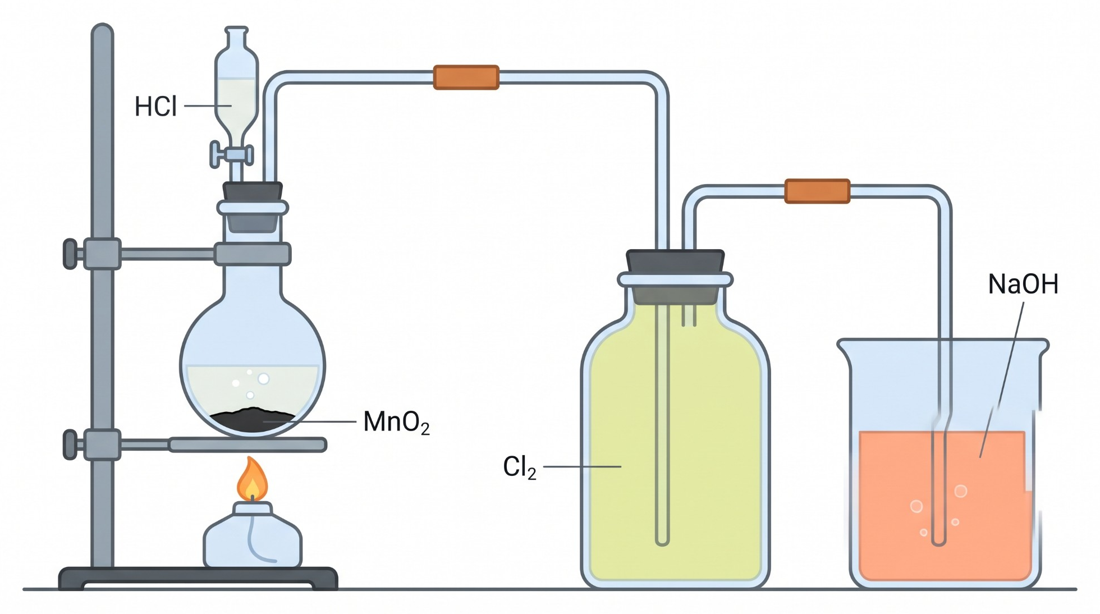
\includegraphics[width=0.86\linewidth]{rasmlar/darslik/d_xlor.png}\end{center}
\noindent A)~\textsl{MnO\textsubscript{2} va konsentrlangan HCl}\par
\noindent B)~\textsl{Zn va HCl}\par
\noindent C)~\textsl{CaCO\textsubscript{3} va HCl}\par
\noindent D)~\textsl{NH\textsubscript{4}Cl va Ca(OH)\textsubscript{2}}\par
\qsep
\noindent\qn{32.} Fenolftalein indikatori kislotali muhitda qanday rang beradi?
\noindent A)~\textsl{malina rangga kiradi (pushti)}\par
\noindent B)~\textsl{sariq}\par
\noindent C)~\textsl{rangsiz}\par
\noindent D)~\textsl{ko`k   ---}\par
\qsep
\end{multicols}
\medskip
\noindent\setlength{\fboxsep}{0pt}\fbox{\begin{tabular}{p{0.74\linewidth}|p{0.2\linewidth}}
\parbox[t]{0.72\linewidth}{\vspace{3pt}\textbf{Topshiriqlar (33--35) va javob variant (A--F)larini o`zaro to`g`ri moslashtiring.} Metan (CH\textsubscript{4}) va eten (C\textsubscript{2}H\textsubscript{4}) dan iborat 10,08 l (n.sh.) aralashma bromli suvdan o`tkazilganda 24 g brom yutildi.
\vspace{3pt}} & \parbox[t]{0.19\linewidth}{\vspace{3pt}A~\textsl{3,36}\\[3pt]
B~\textsl{1,68}\\[3pt]
C~\textsl{6,72}\\[3pt]
D~\textsl{112}\\[3pt]
E~\textsl{33,33}\\[3pt]
F~\textsl{26,67}}\\ \hline
\parbox[t]{0.72\linewidth}{\vspace{2pt}\textbf{33. Aralashmadagi eten (C\textsubscript{2}H\textsubscript{4}) hajmini (l, n.sh.) aniqlang.}\vspace{2pt}} & \\ \hline
\parbox[t]{0.72\linewidth}{\vspace{2pt}\textbf{34. Aralashmadagi eten (C\textsubscript{2}H\textsubscript{4}) hajmiy ulushini (\%) aniqlang.}\vspace{2pt}} & \\ \hline
\parbox[t]{0.72\linewidth}{\vspace{2pt}\textbf{35. Aralashmani to`liq yoqish uchun zarur havo hajmini (l, n.sh.; havoda 21\% kislorod bor) aniqlang.}\vspace{2pt}} & 
\end{tabular}}
\par\bigskip
\noindent\qn{36.} P + HNO\textsubscript{3} + H\textsubscript{2}O $\to$ H\textsubscript{3}PO\textsubscript{4} + NO reaksiya tenglamasini tenglang va barcha koeffitsiyentlar \textbf{yig`indisini aniqlang.}
\javob\qsep
\noindent\qn{37.} 5,6 g Fe reaksiyaga kirishdi (Fe + 2HCl $\to$ FeCl\textsubscript{2} + H\textsubscript{2}). Ajralgan H\textsubscript{2} \textbf{hajmini (l, n.sh.) hisoblang.}
\javob\qsep
\noindent\qn{38.} Alyuminiy va magniy dan iborat 12,9 g aralashma mo`l NaOH eritmasida eritilganda 10,08 l (n.sh.) gaz ajraldi. Aralashmadagi magniy ning massa \textbf{ulushini (\%) aniqlang.}
\javob\qsep
\noindent\qn{39.} C\textsubscript{3}H\textsubscript{7}OH va C\textsubscript{2}H\textsubscript{5}OH dan iborat 15,2 g aralashma natriy bilan to`liq reaksiyaga kirishganda ajraladigan vodorod \textbf{hajmini (l, n.sh.) toping.}
\javob\qsep
\noindent\qn{40.} Vinilxlorid monomeridan olingan polimerning polimerlanish darajasi 2500 bo`lsa, uning molyar \textbf{massasini (g/mol) aniqlang.}
\javob\qsep
\par\bigskip\begin{center}\textbf{\fontsize{13}{15}\selectfont YOZMA ISH}\end{center}
\noindent\qn{41.} \textbf{Topshiriqni bajarish jarayonida barcha reaksiya tenglamalarini yozing. Miqdoriy va arifmetik hisoblashlarni (unga asos bo`lgan usul yoki formulani ko`rsatgan holda) uzviy ketma-ketlikda bajaring.}\par\smallskip
Ketma-ket ulangan ikkita elektrolizyorda CuCl\textsubscript{2} va AgNO\textsubscript{3} eritmalari inert elektrodlar bilan elektroliz qilindi. Birinchi elektrolizyorning katodida 3,2 g Cu ajraldi (F = 96500 C/mol).\par
\noindent 1)\ Elektrolizyordan o`tgan zaryad miqdorini (C) hisoblang.\par
\noindent 2)\ Tok kuchi 5 A bo`lsa, elektroliz necha sekund davom etgan? O`tgan elektronlar miqdorini (mol) ham toping.\par
\noindent 3)\ Ikkinchi elektrolizyorning katodida ajralgan Ag massasini (g) aniqlang.\par
\noindent 4)\ Birinchi elektrolizyor anodida ajralgan gaz hajmini (l, n.sh.) toping. Ikkinchi elektrolizyor katodida ajralgan metallning miqdorini (mol) ham toping.\par
\noindent 5)\ Ikkala elektrolizyorda o`tgan elektronlar sonini (mol) taqqoslab, ularning teng ekanligini isbotlang. Agar tok kuchi 2 marta oshirilsa, shuncha zaryad o`tishi uchun necha sekund kerak?\par
\diqqat{Mazkur topshiriq kengaytirilgan javobni talab etib, uning yechilish usuli va shu usul asosidagi barcha hisoblash amallari javoblar varaqasida aks etishi lozim.}\qsep
\noindent\qn{42.} Quyidagi o`zgarishlar zanjirida \textit{X}, \textit{Y}, \textit{Z} noma'lum organik moddalar:\par
\[\setlength{\fboxsep}{0pt}\text{C\textsubscript{2}H\textsubscript{4}}\xrightarrow{\text{H\textsubscript{2}O, H\textsuperscript{+}}}\text{\textit{X}}\xrightarrow{\text{CuO, t\textdegree{}}}\text{\textit{Y}}\xrightarrow{\text{Ag\textsubscript{2}O, NH\textsubscript{3}}}\text{\textit{Z}}\xrightarrow{\text{C\textsubscript{2}H\textsubscript{5}OH, H\textsubscript{2}SO\textsubscript{4}}}\text{CH\textsubscript{3}COOC\textsubscript{2}H\textsubscript{5}}\]
\noindent 1)\ C\textsubscript{2}H\textsubscript{4} $\to$ \textit{X} : reaksiya tenglamasini yozing; hosil bo`lgan moddani nomlang.\par
\noindent 2)\ \textit{X} $\to$ \textit{Y} : reaksiya tenglamasini yozing; hosil bo`lgan moddani nomlang.\par
\noindent 3)\ \textit{Y} $\to$ \textit{Z} : reaksiya tenglamasini yozing; hosil bo`lgan moddani nomlang.\par
\noindent 4)\ \textit{Z} $\to$ CH\textsubscript{3}COOC\textsubscript{2}H\textsubscript{5} : reaksiya tenglamasini yozing; hosil bo`lgan moddani nomlang.\par
\diqqat{Mazkur topshiriq kengaytirilgan javobni talab etib, uning yechilish usuli va shu usul asosidagi barcha hisoblash amallari javoblar varaqasida aks etishi lozim.}\qsep
\noindent\qn{43.} \textbf{Topshiriqni bajarish jarayonida barcha reaksiya tenglamalarini yozing. Miqdoriy va arifmetik hisoblashlarni (unga asos bo`lgan usul yoki formulani ko`rsatgan holda) uzviy ketma-ketlikda bajaring.}\par\smallskip
Magniy (Mg) va alyuminiy (Al) dan iborat 6,45 g qotishma mo`l suyultirilgan sulfat kislotada eritildi, bunda 7,28 l (n.sh.) gaz ajraldi. Hosil bo`lgan eritmaga mo`l NaOH eritmasi qo`shildi, hosil bo`lgan cho`kma ajratib olindi va havoda qizdirib quritildi.\par
\noindent 1)\ Reaksiya tenglamalarini yozing va qotishmadagi har bir metallning massasini (g) aniqlang.\par
\noindent 2)\ Qotishmadagi Mg ning massa ulushini (\%) hisoblang.\par
\noindent 3)\ Eritish uchun sarflangan 20\% li H\textsubscript{2}SO\textsubscript{4} eritmasining massasini (g) aniqlang.\par
\noindent 4)\ Mo`l NaOH qo`shilganda hosil bo`lgan cho`kmaning formulasi va massasini (g) toping (reaksiya tenglamalarini yozing).\par
\noindent 5)\ Cho`kma havoda to`liq qizdirilganda hosil bo`lgan oksidning massasini (g) hisoblang.\par
\diqqat{Mazkur topshiriq kengaytirilgan javobni talab etib, uning yechilish usuli va shu usul asosidagi barcha hisoblash amallari javoblar varaqasida aks etishi lozim.}\qsep
\newpage\renewcommand{\curvar}{}\thispagestyle{first}
\vspace*{6cm}\begin{center}{\color{ygreen}\rule{0.6\linewidth}{1.6pt}}\\[14pt]{\fontsize{34}{38}\selectfont\bfseries JAVOBLAR}\\[10pt]{\large 1--20-variantlar javoblar kaliti}\\[14pt]{\color{ygreen}\rule{0.6\linewidth}{1.6pt}}\end{center}
\renewcommand{\curvar}{Javoblar}
\newpage
\noindent\textbf{\fontsize{13}{15}\selectfont 1-variant}\hfill \textbf{Javoblar kaliti}\par\smallskip\hrule\smallskip
\textit{Faqat o`qituvchi uchun.}\par\medskip
\noindent\textbf{1--32-savollar}\par\smallskip
\noindent\begin{tabular}{|c|c|c|c|c|c|c|c|c|c|c|c|c|c|c|c|}\hline
\textbf{1} & \textbf{2} & \textbf{3} & \textbf{4} & \textbf{5} & \textbf{6} & \textbf{7} & \textbf{8} & \textbf{9} & \textbf{10} & \textbf{11} & \textbf{12} & \textbf{13} & \textbf{14} & \textbf{15} & \textbf{16}\\\hline
\textsl{A} & \textsl{C} & \textsl{C} & \textsl{D} & \textsl{D} & \textsl{C} & \textsl{A} & \textsl{A} & \textsl{B} & \textsl{C} & \textsl{B} & \textsl{B} & \textsl{B} & \textsl{C} & \textsl{C} & \textsl{D}\\\hline
\textbf{17} & \textbf{18} & \textbf{19} & \textbf{20} & \textbf{21} & \textbf{22} & \textbf{23} & \textbf{24} & \textbf{25} & \textbf{26} & \textbf{27} & \textbf{28} & \textbf{29} & \textbf{30} & \textbf{31} & \textbf{32}\\\hline
\textsl{D} & \textsl{B} & \textsl{D} & \textsl{A} & \textsl{D} & \textsl{D} & \textsl{B} & \textsl{B} & \textsl{A} & \textsl{C} & \textsl{A} & \textsl{C} & \textsl{B} & \textsl{A} & \textsl{A} & \textsl{D}\\\hline
\end{tabular}\par\medskip
\noindent\textbf{33--35-savollar}\par\smallskip
\noindent\begin{tabular}{|c|c|c|}\hline \textbf{No} & \textbf{Javob} & \textbf{Qiymat}\\\hline
33 & \textsl{E} & 10,86\\\hline
34 & \textsl{B} & 85,33\\\hline
35 & \textsl{A} & 7,04\\\hline
\end{tabular}\par\medskip
\noindent\textbf{36--40-savollar}\par\smallskip
\noindent\begin{tabular}{|c|c|}\hline \textbf{No} & \textbf{To`g`ri javob}\\\hline
36 & 18\\\hline
37 & 3\\\hline
38 & 8\\\hline
39 & 6\\\hline
40 & 14,69\\\hline
\end{tabular}\par\medskip
\noindent\textbf{41--43-topshiriqlar: javoblar}\par\smallskip
\noindent\textbf{41-topshiriq.}\par
\noindent 1) 5,306 mol/l\par
\noindent 2) 10,612 ekv/l; 49 g/ekv\par
\noindent 3) 6,803 mol/kg\par
\noindent 4) 9,42 ml; 78 g\par
\noindent 5) 42,45 g; 130 g\par
\noindent\textbf{42-topshiriq.}\par
\noindent 1) CH\textsubscript{3}CHO + Ag\textsubscript{2}O, NH\textsubscript{3} $\to$ CH\textsubscript{3}COOH (sirka kislota)\par
\noindent 2) CH\textsubscript{3}COOH + C\textsubscript{2}H\textsubscript{5}OH, H\textsubscript{2}SO\textsubscript{4} $\to$ CH\textsubscript{3}COOC\textsubscript{2}H\textsubscript{5} (etilatsetat)\par
\noindent 3) CH\textsubscript{3}COOC\textsubscript{2}H\textsubscript{5} + NaOH $\to$ CH\textsubscript{3}COONa (natriy atsetat)\par
\noindent 4) CH\textsubscript{3}COONa + NaOH (suyuqlanma), t\textdegree{} $\to$ CH\textsubscript{4} (metan)\par
\noindent\textbf{43-topshiriq.}\par
\noindent 1) 19,6 g; 4,48 l\par
\noindent 2) 46,6 g\par
\noindent 3) 19,7 g\par
\noindent 4) 57,33 g/mol; 1,98\par
\noindent 5) 32,4 g\par
\par\bigskip\noindent\textbf{Mavzular taqsimoti}\par\smallskip
{\small\noindent\begin{longtable}{|c|p{7.2cm}|p{5.4cm}|c|}\hline \textbf{No} & \textbf{Mavzu} & \textbf{Tekshiriladigan ko`nikma} & \textbf{Ball}\\\hline
1 & 8-sinf (izotoplar, izobarlar, jadval) & Jadval tahlili & 1\\\hline
2 & Tirkashev III bob (eritmalar) & Hisoblash va masala yechish & 1\\\hline
3 & 8-sinf; Tirkashev \textit{V} bob (oksidlanish darajasi) & Bilim va tushunish & 1\\\hline
4 & 8-sinf (havo tarkibi, diagramma) & Grafik tahlili & 1\\\hline
5 & Tirkashev VI bob (muvozanat, jadval) & Jadval tahlili & 1\\\hline
6 & 9-sinf; Tirkashev IV bob (dissotsilanish darajasi) & Hisoblash va masala yechish & 1\\\hline
7 & 7-sinf (mol) & Hisoblash va masala yechish & 1\\\hline
8 & Tirkashev VI bob (Le-Shatelye) & Bilim va tushunish & 1\\\hline
9 & Tirkashev III bob (eruvchanlik, jadval) & Jadval tahlili & 1\\\hline
10 & 8-sinf; Tirkashev II bob (kimyoviy bog`lanish) & Bilim va tushunish & 1\\\hline
11 & Tirkashev I bob; 8-sinf (elektron konfiguratsiya) & Bilim va tushunish & 1\\\hline
12 & Tirkashev I bob; 8-sinf (izoelektron) & Bilim va tushunish & 1\\\hline
13 & Tirkashev \textit{V} bob; 11-sinf 7-bob (OQR tenglash) & Hisoblash va masala yechish & 1\\\hline
14 & 9-sinf; Tirkashev (P/C/Si, hisob) & Hisoblash va masala yechish & 1\\\hline
15 & Tashev (galogenlar) & Hisoblash va masala yechish & 1\\\hline
16 & 9-sinf; Tirkashev (IA metallar, hisob) & Hisoblash va masala yechish & 1\\\hline
17 & 9-sinf (metallar aktivligi) & Rasm bo`yicha tahlil & 1\\\hline
18 & 9-sinf; Tashev (Fe, Cu, Zn, Cr) & Bilim va tushunish & 1\\\hline
19 & 9-sinf \S{}24 (doimiy qattiqlik, soda) & Hisoblash va masala yechish & 1\\\hline
20 & 10-sinf (nomenklatura \S{}6, \S{}11, \S{}20, \S{}24--26) & Bilim va tushunish & 1\\\hline
21 & 10-sinf \S{}14; Abdusamatov (Lebedev) & Hisoblash va masala yechish & 1\\\hline
22 & 10-sinf (mavzuga oid paragraflar); Abdusamatov & Bilim va tushunish & 1\\\hline
23 & 10-sinf (spirt, hisob) & Hisoblash va masala yechish & 1\\\hline
24 & 10-sinf (ald, hisob) & Hisoblash va masala yechish & 1\\\hline
25 & 10-sinf (mavzuga oid paragraflar); Abdusamatov & Bilim va tushunish & 1\\\hline
26 & 10-sinf \S{}28 & Hisoblash va masala yechish & 1\\\hline
27 & 10-sinf (mavzuga oid paragraflar); Abdusamatov & Bilim va tushunish & 1\\\hline
28 & 10-sinf \S{}33 & Hisoblash va masala yechish & 1\\\hline
29 & 10-sinf (olinish usullari) & Bilim va tushunish & 1\\\hline
30 & 8-sinf (19-rasm; eritmalar) & Rasm bo`yicha tahlil & 1\\\hline
31 & 8-sinf (indikatorlar) & Bilim va tushunish & 1\\\hline
32 & 9--10-sinf (laboratoriya usullari bilan gaz olish) & Bilim va tushunish & 1\\\hline
33--35 & Aralash masala (moslashtirish) & Ko`p bosqichli hisob & 3\\\hline
36--40 & Qisqa javobli masalalar & Hisoblash & 5\\\hline
41--43 & Yozma ish & Usul va hisob (M, A) & 75\\\hline
\end{longtable}}
\renewcommand{\curvar}{Javoblar}
\newpage
\noindent\textbf{\fontsize{13}{15}\selectfont 2-variant}\hfill \textbf{Javoblar kaliti}\par\smallskip\hrule\smallskip
\textit{Faqat o`qituvchi uchun.}\par\medskip
\noindent\textbf{1--32-savollar}\par\smallskip
\noindent\begin{tabular}{|c|c|c|c|c|c|c|c|c|c|c|c|c|c|c|c|}\hline
\textbf{1} & \textbf{2} & \textbf{3} & \textbf{4} & \textbf{5} & \textbf{6} & \textbf{7} & \textbf{8} & \textbf{9} & \textbf{10} & \textbf{11} & \textbf{12} & \textbf{13} & \textbf{14} & \textbf{15} & \textbf{16}\\\hline
\textsl{A} & \textsl{B} & \textsl{D} & \textsl{D} & \textsl{B} & \textsl{C} & \textsl{C} & \textsl{B} & \textsl{D} & \textsl{D} & \textsl{D} & \textsl{C} & \textsl{A} & \textsl{C} & \textsl{A} & \textsl{D}\\\hline
\textbf{17} & \textbf{18} & \textbf{19} & \textbf{20} & \textbf{21} & \textbf{22} & \textbf{23} & \textbf{24} & \textbf{25} & \textbf{26} & \textbf{27} & \textbf{28} & \textbf{29} & \textbf{30} & \textbf{31} & \textbf{32}\\\hline
\textsl{A} & \textsl{B} & \textsl{B} & \textsl{B} & \textsl{A} & \textsl{B} & \textsl{C} & \textsl{B} & \textsl{C} & \textsl{C} & \textsl{A} & \textsl{A} & \textsl{C} & \textsl{D} & \textsl{A} & \textsl{D}\\\hline
\end{tabular}\par\medskip
\noindent\textbf{33--35-savollar}\par\smallskip
\noindent\begin{tabular}{|c|c|c|}\hline \textbf{No} & \textbf{Javob} & \textbf{Qiymat}\\\hline
33 & \textsl{A} & 8,3\\\hline
34 & \textsl{F} & 255\\\hline
35 & \textsl{C} & 13,55\\\hline
\end{tabular}\par\medskip
\noindent\textbf{36--40-savollar}\par\smallskip
\noindent\begin{tabular}{|c|c|}\hline \textbf{No} & \textbf{To`g`ri javob}\\\hline
36 & 36\\\hline
37 & 4,48\\\hline
38 & 5,6\\\hline
39 & 25,6\\\hline
40 & 180\\\hline
\end{tabular}\par\medskip
\noindent\textbf{41--43-topshiriqlar: javoblar}\par\smallskip
\noindent\textbf{41-topshiriq.}\par
\noindent 1) 50 g; 64,4 g\par
\noindent 2) 7,72\%; 6,85\%; 38600 C\par
\noindent 3) 2,24 l; 398,4 g\par
\noindent 4) 4,92\%; 7,13\%; 32 g\par
\noindent 5) 65,6 ml; 3860 s\par
\noindent\textbf{42-topshiriq.}\par
\noindent 1) CH\textsubscript{3}Cl + Na $\to$ C\textsubscript{2}H\textsubscript{6} (etan)\par
\noindent 2) C\textsubscript{2}H\textsubscript{6} + Cl\textsubscript{2}, yorug`lik $\to$ C\textsubscript{2}H\textsubscript{5}Cl (xloretan)\par
\noindent 3) C\textsubscript{2}H\textsubscript{5}Cl + KOH (suvli) $\to$ C\textsubscript{2}H\textsubscript{5}OH (etanol)\par
\noindent\textbf{43-topshiriq.}\par
\noindent 1) Ca(HCO\textsubscript{3})\textsubscript{2} $\to$ CaCO\textsubscript{3}$\downarrow$ + CO\textsubscript{2}$\uparrow$ + H\textsubscript{2}O; Mg(HCO\textsubscript{3})\textsubscript{2} $\to$ MgCO\textsubscript{3}$\downarrow$ + CO\textsubscript{2}$\uparrow$ + H\textsubscript{2}O\par
\noindent 2) 200 kg; 56 m\textsuperscript{3}\par
\noindent 3) 42 kg\par
\noindent 4) 265 kg\par
\noindent 5) 222 kg\par
\par\bigskip\noindent\textbf{Mavzular taqsimoti}\par\smallskip
{\small\noindent\begin{longtable}{|c|p{7.2cm}|p{5.4cm}|c|}\hline \textbf{No} & \textbf{Mavzu} & \textbf{Tekshiriladigan ko`nikma} & \textbf{Ball}\\\hline
1 & Tirkashev III bob (eritmalar, jadval) & Jadval tahlili & 1\\\hline
2 & 7-sinf; Tirkashev (kristallogidrat) & Hisoblash va masala yechish & 1\\\hline
3 & 8-sinf (davriy qonun, diagramma) & Grafik tahlili & 1\\\hline
4 & 11-sinf (yadro reaksiyalari) & Rasm bo`yicha tahlil & 1\\\hline
5 & Tirkashev III bob (oleum); Tashev & Hisoblash va masala yechish & 1\\\hline
6 & Tirkashev VI bob (kimyoviy muvozanat) & Hisoblash va masala yechish & 1\\\hline
7 & Tirkashev IV bob (kuchli elektrolitlar) & Hisoblash va masala yechish & 1\\\hline
8 & Tirkashev \textit{V} bob (kuchlanish qatori, jadval) & Jadval tahlili & 1\\\hline
9 & 8-sinf (Gey-Lyussak qonuni) & Hisoblash va masala yechish & 1\\\hline
10 & 11-sinf (ekvivalentlar qonuni) & Hisoblash va masala yechish & 1\\\hline
11 & Tirkashev I bob; 8-sinf (elektron konfiguratsiya) & Bilim va tushunish & 1\\\hline
12 & 11-sinf 4-bob (molyar konsentratsiya) & Hisoblash va masala yechish & 1\\\hline
13 & 8-sinf; 9-sinf (stexiometriya) & Hisoblash va masala yechish & 1\\\hline
14 & 9-sinf (ishqoriy metallar); Tashev & Bilim va tushunish & 1\\\hline
15 & 9-sinf; Tirkashev (IIA/IIIA metallar (Ca,Mg,Al), hisob) & Hisoblash va masala yechish & 1\\\hline
16 & 9-sinf; Tashev (temir) & Hisoblash va masala yechish & 1\\\hline
17 & 9-sinf; Tirkashev (suv qattiqligi, hisob) & Hisoblash va masala yechish & 1\\\hline
18 & 9-sinf; Tashev (anorganik birikmalar xossalari) & Bilim va tushunish & 1\\\hline
19 & 9-sinf; Tirkashev (genetik zanjir/reaksiya turlari, hisob) & Hisoblash va masala yechish & 1\\\hline
20 & 10-sinf \S{}6, \S{}12, \S{}20, \S{}28 (izomeriya) & Bilim va tushunish & 1\\\hline
21 & 10-sinf \S{}21 (etilen olinishi) & Hisoblash va masala yechish & 1\\\hline
22 & 10-sinf (mavzuga oid paragraflar); Abdusamatov & Bilim va tushunish & 1\\\hline
23 & 10-sinf (mavzuga oid paragraflar); Abdusamatov & Bilim va tushunish & 1\\\hline
24 & 10-sinf (ald, hisob) & Hisoblash va masala yechish & 1\\\hline
25 & 10-sinf (ikki bosqichli hisob) & Hisoblash va masala yechish & 1\\\hline
26 & 10-sinf \S{}29 (yog`lar, sovunlanish) & Hisoblash va masala yechish & 1\\\hline
27 & 10-sinf (ikki bosqichli hisob) & Hisoblash va masala yechish & 1\\\hline
28 & 10-sinf (ikki bosqichli hisob) & Hisoblash va masala yechish & 1\\\hline
29 & 10-sinf (olinish usullari) & Bilim va tushunish & 1\\\hline
30 & 7--10-sinf va Tashev (laboratoriya ishlari, sifat reaksiyalar) & Jadval tahlili & 1\\\hline
31 & 7-sinf (laboratoriya jihozlari, 3-rasm) & Rasm bo`yicha tahlil & 1\\\hline
32 & Tirkashev III bob (eritmalar) & Hisoblash va masala yechish & 1\\\hline
33--35 & Aralash masala (moslashtirish) & Ko`p bosqichli hisob & 3\\\hline
36--40 & Qisqa javobli masalalar & Hisoblash & 5\\\hline
41--43 & Yozma ish & Usul va hisob (M, A) & 75\\\hline
\end{longtable}}
\renewcommand{\curvar}{Javoblar}
\newpage
\noindent\textbf{\fontsize{13}{15}\selectfont 3-variant}\hfill \textbf{Javoblar kaliti}\par\smallskip\hrule\smallskip
\textit{Faqat o`qituvchi uchun.}\par\medskip
\noindent\textbf{1--32-savollar}\par\smallskip
\noindent\begin{tabular}{|c|c|c|c|c|c|c|c|c|c|c|c|c|c|c|c|}\hline
\textbf{1} & \textbf{2} & \textbf{3} & \textbf{4} & \textbf{5} & \textbf{6} & \textbf{7} & \textbf{8} & \textbf{9} & \textbf{10} & \textbf{11} & \textbf{12} & \textbf{13} & \textbf{14} & \textbf{15} & \textbf{16}\\\hline
\textsl{B} & \textsl{D} & \textsl{B} & \textsl{D} & \textsl{A} & \textsl{D} & \textsl{A} & \textsl{C} & \textsl{C} & \textsl{B} & \textsl{D} & \textsl{C} & \textsl{B} & \textsl{C} & \textsl{B} & \textsl{B}\\\hline
\textbf{17} & \textbf{18} & \textbf{19} & \textbf{20} & \textbf{21} & \textbf{22} & \textbf{23} & \textbf{24} & \textbf{25} & \textbf{26} & \textbf{27} & \textbf{28} & \textbf{29} & \textbf{30} & \textbf{31} & \textbf{32}\\\hline
\textsl{A} & \textsl{B} & \textsl{D} & \textsl{A} & \textsl{A} & \textsl{D} & \textsl{C} & \textsl{C} & \textsl{D} & \textsl{A} & \textsl{D} & \textsl{B} & \textsl{C} & \textsl{A} & \textsl{A} & \textsl{C}\\\hline
\end{tabular}\par\medskip
\noindent\textbf{33--35-savollar}\par\smallskip
\noindent\begin{tabular}{|c|c|c|}\hline \textbf{No} & \textbf{Javob} & \textbf{Qiymat}\\\hline
33 & \textsl{A} & 10,2\\\hline
34 & \textsl{B} & 164,25\\\hline
35 & \textsl{F} & 40,05\\\hline
\end{tabular}\par\medskip
\noindent\textbf{36--40-savollar}\par\smallskip
\noindent\begin{tabular}{|c|c|}\hline \textbf{No} & \textbf{To`g`ri javob}\\\hline
36 & 3\\\hline
37 & 3,56\\\hline
38 & 111\\\hline
39 & 12,4\\\hline
40 & 72\\\hline
\end{tabular}\par\medskip
\noindent\textbf{41--43-topshiriqlar: javoblar}\par\smallskip
\noindent\textbf{41-topshiriq.}\par
\noindent 1) 1$\cdot$10\textsuperscript{$-$}10\par
\noindent 2) 1$\cdot$10\textsuperscript{$-$}5 mol/l; 5\par
\noindent 3) pH = 9\par
\noindent 4) 0,001\%; 1$\cdot$10\textsuperscript{$-$}9 mol/l\par
\noindent 5) 34 g; 3,16 marta\par
\noindent\textbf{42-topshiriq.}\par
\noindent 1) CH\textsubscript{3}COOC\textsubscript{2}H\textsubscript{5} + NaOH $\to$ CH\textsubscript{3}COONa (natriy atsetat)\par
\noindent 2) CH\textsubscript{3}COONa + NaOH (suyuqlanma), t\textdegree{} $\to$ CH\textsubscript{4} (metan)\par
\noindent 3) CH\textsubscript{4} + Cl\textsubscript{2}, yorug`lik $\to$ CH\textsubscript{3}Cl (xlormetan)\par
\noindent\textbf{43-topshiriq.}\par
\noindent 1) $-$0,1 g\par
\noindent 2) 47,4\%\par
\noindent 3) 21,4 g\par
\noindent 4) 17,9 g\par
\noindent 5) 8 g\par
\par\bigskip\noindent\textbf{Mavzular taqsimoti}\par\smallskip
{\small\noindent\begin{longtable}{|c|p{7.2cm}|p{5.4cm}|c|}\hline \textbf{No} & \textbf{Mavzu} & \textbf{Tekshiriladigan ko`nikma} & \textbf{Ball}\\\hline
1 & Tirkashev I bob (kvant sonlari) & Bilim va tushunish & 1\\\hline
2 & Tirkashev VI bob (muvozanat, jadval) & Jadval tahlili & 1\\\hline
3 & Tirkashev III bob & Hisoblash va masala yechish & 1\\\hline
4 & Tirkashev VI bob (Le-Shatelye) & Bilim va tushunish & 1\\\hline
5 & Tirkashev \textit{V} bob; Tashev (HNO\textsubscript{3}, H\textsubscript{2}SO\textsubscript{4}) & Hisoblash va masala yechish & 1\\\hline
6 & Tirkashev IV bob (kuchli elektrolitlar) & Hisoblash va masala yechish & 1\\\hline
7 & Tirkashev VI bob & Hisoblash va masala yechish & 1\\\hline
8 & Tirkashev VI bob (reaksiya tezligi, grafik) & Grafik tahlili & 1\\\hline
9 & 8-sinf (ortiqcha modda masalasi) & Hisoblash va masala yechish & 1\\\hline
10 & Tirkashev I bob; 8-sinf (izoelektron) & Bilim va tushunish & 1\\\hline
11 & 11-sinf 8-bob; Tirkashev \textit{V} bob (elektroliz) & Bilim va tushunish & 1\\\hline
12 & 8-sinf (kimyoviy bog`lanish turlari, jadval) & Jadval tahlili & 1\\\hline
13 & Tirkashev IV bob (kuchli elektrolitlar) & Hisoblash va masala yechish & 1\\\hline
14 & 9-sinf; Tirkashev (d-metallar (Fe,Cu,Zn,Cr), hisob) & Hisoblash va masala yechish & 1\\\hline
15 & 9-sinf \S{}24 (suv qattiqligi) & Hisoblash va masala yechish & 1\\\hline
16 & 9-sinf; Tirkashev (oksid/asos/kislota/tuz, hisob) & Hisoblash va masala yechish & 1\\\hline
17 & 9-sinf; Tashev (anorganik birikmalar xossalari) & Bilim va tushunish & 1\\\hline
18 & 9-sinf; Tirkashev (mineral o`g`itlar/nodir gazlar, hisob) & Hisoblash va masala yechish & 1\\\hline
19 & Tashev (nitratlar) & Bilim va tushunish & 1\\\hline
20 & 10-sinf (nomenklatura \S{}6, \S{}11, \S{}20, \S{}24--26) & Bilim va tushunish & 1\\\hline
21 & 10-sinf \S{}13, \S{}15 (alken va alkin birikish reaksiyalari) & Hisoblash va masala yechish & 1\\\hline
22 & 10-sinf \S{}16, \S{}23, \S{}33 & Hisoblash va masala yechish & 1\\\hline
23 & 10-sinf (organik moddalarning o`zaro bog`lanishi) & Rasm bo`yicha tahlil & 1\\\hline
24 & 10-sinf (mavzuga oid paragraflar); Abdusamatov & Bilim va tushunish & 1\\\hline
25 & 10-sinf (mavzuga oid paragraflar); Abdusamatov & Bilim va tushunish & 1\\\hline
26 & 10-sinf \S{}28 (efirlar gidrolizi) & Hisoblash va masala yechish & 1\\\hline
27 & 10-sinf (ikki bosqichli hisob) & Hisoblash va masala yechish & 1\\\hline
28 & 10-sinf \S{}33 & Hisoblash va masala yechish & 1\\\hline
29 & 10-sinf \S{}35 (YuMB) & Hisoblash va masala yechish & 1\\\hline
30 & 8-sinf (indikatorlar) & Bilim va tushunish & 1\\\hline
31 & 7-sinf (10-rasm) & Rasm bo`yicha tahlil & 1\\\hline
32 & 9--10-sinf (laboratoriya usullari bilan gaz olish) & Bilim va tushunish & 1\\\hline
33--35 & Aralash masala (moslashtirish) & Ko`p bosqichli hisob & 3\\\hline
36--40 & Qisqa javobli masalalar & Hisoblash & 5\\\hline
41--43 & Yozma ish & Usul va hisob (M, A) & 75\\\hline
\end{longtable}}
\renewcommand{\curvar}{Javoblar}
\newpage
\noindent\textbf{\fontsize{13}{15}\selectfont 4-variant}\hfill \textbf{Javoblar kaliti}\par\smallskip\hrule\smallskip
\textit{Faqat o`qituvchi uchun.}\par\medskip
\noindent\textbf{1--32-savollar}\par\smallskip
\noindent\begin{tabular}{|c|c|c|c|c|c|c|c|c|c|c|c|c|c|c|c|}\hline
\textbf{1} & \textbf{2} & \textbf{3} & \textbf{4} & \textbf{5} & \textbf{6} & \textbf{7} & \textbf{8} & \textbf{9} & \textbf{10} & \textbf{11} & \textbf{12} & \textbf{13} & \textbf{14} & \textbf{15} & \textbf{16}\\\hline
\textsl{B} & \textsl{C} & \textsl{A} & \textsl{B} & \textsl{D} & \textsl{A} & \textsl{C} & \textsl{C} & \textsl{B} & \textsl{B} & \textsl{C} & \textsl{A} & \textsl{A} & \textsl{B} & \textsl{B} & \textsl{D}\\\hline
\textbf{17} & \textbf{18} & \textbf{19} & \textbf{20} & \textbf{21} & \textbf{22} & \textbf{23} & \textbf{24} & \textbf{25} & \textbf{26} & \textbf{27} & \textbf{28} & \textbf{29} & \textbf{30} & \textbf{31} & \textbf{32}\\\hline
\textsl{D} & \textsl{A} & \textsl{A} & \textsl{B} & \textsl{D} & \textsl{D} & \textsl{D} & \textsl{D} & \textsl{C} & \textsl{C} & \textsl{C} & \textsl{A} & \textsl{B} & \textsl{A} & \textsl{D} & \textsl{C}\\\hline
\end{tabular}\par\medskip
\noindent\textbf{33--35-savollar}\par\smallskip
\noindent\begin{tabular}{|c|c|c|}\hline \textbf{No} & \textbf{Javob} & \textbf{Qiymat}\\\hline
33 & \textsl{D} & 2,24\\\hline
34 & \textsl{C} & 33,33\\\hline
35 & \textsl{A} & 138,67\\\hline
\end{tabular}\par\medskip
\noindent\textbf{36--40-savollar}\par\smallskip
\noindent\begin{tabular}{|c|c|}\hline \textbf{No} & \textbf{To`g`ri javob}\\\hline
36 & 5\\\hline
37 & 2\\\hline
38 & 3,36\\\hline
39 & 3,96\\\hline
40 & 186,67\\\hline
\end{tabular}\par\medskip
\noindent\textbf{41--43-topshiriqlar: javoblar}\par\smallskip
\noindent\textbf{41-topshiriq.}\par
\noindent 1) 29\par
\noindent 2) 58,8 g; 0,2 mol\par
\noindent 3) 2,8 mol; 1,2 mol\par
\noindent 4) 76,2 g; 99,6 g\par
\noindent 5) 12,25 g; 22,35 g\par
\noindent\textbf{42-topshiriq.}\par
\noindent 1) CaC\textsubscript{2} + H\textsubscript{2}O $\to$ C\textsubscript{2}H\textsubscript{2} (asetilen)\par
\noindent 2) C\textsubscript{2}H\textsubscript{2} + C (aktiv), 600 \textdegree{}C $\to$ C\textsubscript{6}H\textsubscript{6} (benzol)\par
\noindent 3) C\textsubscript{6}H\textsubscript{6} + HNO\textsubscript{3}, H\textsubscript{2}SO\textsubscript{4} $\to$ C\textsubscript{6}H\textsubscript{5}NO\textsubscript{2} (nitrobenzol)\par
\noindent 4) C\textsubscript{6}H\textsubscript{5}NO\textsubscript{2} + Fe, HCl $\to$ C\textsubscript{6}H\textsubscript{5}NH\textsubscript{2} (anilin)\par
\noindent\textbf{43-topshiriq.}\par
\noindent 1) 25\%; 1,4 l\par
\noindent 2) 18,3\%\par
\noindent 3) 1,04\%\par
\noindent 4) 12,25 g; 7,58 g\par
\noindent 5) 43,2 g/mol\par
\par\bigskip\noindent\textbf{Mavzular taqsimoti}\par\smallskip
{\small\noindent\begin{longtable}{|c|p{7.2cm}|p{5.4cm}|c|}\hline \textbf{No} & \textbf{Mavzu} & \textbf{Tekshiriladigan ko`nikma} & \textbf{Ball}\\\hline
1 & Tirkashev VI bob (tezlik, jadval) & Jadval tahlili & 1\\\hline
2 & 8-sinf (molyar hajm, grafik) & Grafik tahlili & 1\\\hline
3 & Tirkashev I bob (kvant sonlari) & Bilim va tushunish & 1\\\hline
4 & 8-sinf (Gey-Lyussak, Avogadro) & Hisoblash va masala yechish & 1\\\hline
5 & 8-sinf; Tirkashev \textit{V} bob (oksidlanish darajasi) & Bilim va tushunish & 1\\\hline
6 & 8-sinf (atom tuzilishi) & Hisoblash va masala yechish & 1\\\hline
7 & Tirkashev VI bob & Hisoblash va masala yechish & 1\\\hline
8 & Tirkashev VI bob (Le-Shatelye) & Bilim va tushunish & 1\\\hline
9 & 7-sinf; Tirkashev (kristallogidrat) & Hisoblash va masala yechish & 1\\\hline
10 & 11-sinf 8-bob (Faradey qonunlari); Tirkashev \textit{V} bob & Hisoblash va masala yechish & 1\\\hline
11 & 8-sinf (atom tuzilishi, jadval) & Jadval tahlili & 1\\\hline
12 & Tashev; 9-sinf (kuchlanish qatori) & Bilim va tushunish & 1\\\hline
13 & 11-sinf 4-bob (molyar konsentratsiya) & Hisoblash va masala yechish & 1\\\hline
14 & 9-sinf; Tashev (anorganik birikmalar xossalari) & Bilim va tushunish & 1\\\hline
15 & 9-sinf; Tirkashev (genetik zanjir/reaksiya turlari, hisob) & Hisoblash va masala yechish & 1\\\hline
16 & Tashev (o`g`itlar) & Hisoblash va masala yechish & 1\\\hline
17 & Tashev (nitratlar) & Bilim va tushunish & 1\\\hline
18 & 9-sinf; Tirkashev (S/SO\textsubscript{2}/H\textsubscript{2}SO\textsubscript{4}, hisob) & Hisoblash va masala yechish & 1\\\hline
19 & 9-sinf; Tirkashev (N/NH\textsubscript{3}/HNO\textsubscript{3}, hisob) & Hisoblash va masala yechish & 1\\\hline
20 & 10-sinf (aminokislotalar) & Rasm bo`yicha tahlil & 1\\\hline
21 & 10-sinf (mavzuga oid paragraflar); Abdusamatov & Bilim va tushunish & 1\\\hline
22 & 10-sinf (mavzuga oid paragraflar); Abdusamatov & Bilim va tushunish & 1\\\hline
23 & 10-sinf (mavzuga oid paragraflar); Abdusamatov & Bilim va tushunish & 1\\\hline
24 & 10-sinf (ikki bosqichli hisob) & Hisoblash va masala yechish & 1\\\hline
25 & 10-sinf (mavzuga oid paragraflar); Abdusamatov & Bilim va tushunish & 1\\\hline
26 & 10-sinf (efir, hisob) & Hisoblash va masala yechish & 1\\\hline
27 & 10-sinf (organik birikmalar sinflari) & Bilim va tushunish & 1\\\hline
28 & 10-sinf (amin, hisob) & Hisoblash va masala yechish & 1\\\hline
29 & 10-sinf \S{}35 & Hisoblash va masala yechish & 1\\\hline
30 & 9-sinf (sifat reaksiyalar) & Bilim va tushunish & 1\\\hline
31 & 7--10-sinf va Tashev (laboratoriya ishlari, sifat reaksiyalar) & Jadval tahlili & 1\\\hline
32 & 10-sinf (efirlanish, 8-rasm) & Rasm bo`yicha tahlil & 1\\\hline
33--35 & Aralash masala (moslashtirish) & Ko`p bosqichli hisob & 3\\\hline
36--40 & Qisqa javobli masalalar & Hisoblash & 5\\\hline
41--43 & Yozma ish & Usul va hisob (M, A) & 75\\\hline
\end{longtable}}
\renewcommand{\curvar}{Javoblar}
\newpage
\noindent\textbf{\fontsize{13}{15}\selectfont 5-variant}\hfill \textbf{Javoblar kaliti}\par\smallskip\hrule\smallskip
\textit{Faqat o`qituvchi uchun.}\par\medskip
\noindent\textbf{1--32-savollar}\par\smallskip
\noindent\begin{tabular}{|c|c|c|c|c|c|c|c|c|c|c|c|c|c|c|c|}\hline
\textbf{1} & \textbf{2} & \textbf{3} & \textbf{4} & \textbf{5} & \textbf{6} & \textbf{7} & \textbf{8} & \textbf{9} & \textbf{10} & \textbf{11} & \textbf{12} & \textbf{13} & \textbf{14} & \textbf{15} & \textbf{16}\\\hline
\textsl{B} & \textsl{D} & \textsl{C} & \textsl{C} & \textsl{D} & \textsl{D} & \textsl{B} & \textsl{C} & \textsl{A} & \textsl{D} & \textsl{B} & \textsl{D} & \textsl{D} & \textsl{B} & \textsl{A} & \textsl{B}\\\hline
\textbf{17} & \textbf{18} & \textbf{19} & \textbf{20} & \textbf{21} & \textbf{22} & \textbf{23} & \textbf{24} & \textbf{25} & \textbf{26} & \textbf{27} & \textbf{28} & \textbf{29} & \textbf{30} & \textbf{31} & \textbf{32}\\\hline
\textsl{D} & \textsl{B} & \textsl{C} & \textsl{C} & \textsl{C} & \textsl{D} & \textsl{B} & \textsl{A} & \textsl{A} & \textsl{A} & \textsl{C} & \textsl{B} & \textsl{C} & \textsl{A} & \textsl{A} & \textsl{A}\\\hline
\end{tabular}\par\medskip
\noindent\textbf{33--35-savollar}\par\smallskip
\noindent\begin{tabular}{|c|c|c|}\hline \textbf{No} & \textbf{Javob} & \textbf{Qiymat}\\\hline
33 & \textsl{B} & 6,72\\\hline
34 & \textsl{D} & 0,6\\\hline
35 & \textsl{C} & 10,08\\\hline
\end{tabular}\par\medskip
\noindent\textbf{36--40-savollar}\par\smallskip
\noindent\begin{tabular}{|c|c|}\hline \textbf{No} & \textbf{To`g`ri javob}\\\hline
36 & 12\\\hline
37 & 12\\\hline
38 & 7,5\\\hline
39 & 1,12\\\hline
40 & 16\\\hline
\end{tabular}\par\medskip
\noindent\textbf{41--43-topshiriqlar: javoblar}\par\smallskip
\noindent\textbf{41-topshiriq.}\par
\noindent 1) 63,6\par
\noindent 2) 0,503 mol; 14,591 mol\par
\noindent 3) 0,151 mol\par
\noindent 4) 17,409 mol; 10,56$\cdot$10\textsuperscript{$-$23} g\par
\noindent 5) 3,03$\cdot$10\textsuperscript{23}; 0,838\par
\noindent\textbf{42-topshiriq.}\par
\noindent 1) C\textsubscript{2}H\textsubscript{5}Cl + KOH (suvli) $\to$ C\textsubscript{2}H\textsubscript{5}OH (etanol)\par
\noindent 2) C\textsubscript{2}H\textsubscript{5}OH + H\textsubscript{2}SO\textsubscript{4} (kons.), 170 \textdegree{}C $\to$ C\textsubscript{2}H\textsubscript{4} (etilen)\par
\noindent 3) C\textsubscript{2}H\textsubscript{4} + Br\textsubscript{2} $\to$ C\textsubscript{2}H\textsubscript{4}Br\textsubscript{2} (1,2-dibrometan)\par
\noindent 4) C\textsubscript{2}H\textsubscript{4}Br\textsubscript{2} + KOH (spirtli) $\to$ C\textsubscript{2}H\textsubscript{2} (asetilen)\par
\noindent\textbf{43-topshiriq.}\par
\noindent 1) x$\cdot$100 + y$\cdot$84 = 28,4; x + y = 0,3 $\to$ CaCO\textsubscript{3} 20 g (70,4\%), MgCO\textsubscript{3} 8,4 g (29,6\%)\par
\noindent 2) 6,72 l; 15,2 g; 73,7\%\par
\noindent 3) 30 g\par
\noindent 4) 219 g\par
\noindent 5) 14,8 g\par
\par\bigskip\noindent\textbf{Mavzular taqsimoti}\par\smallskip
{\small\noindent\begin{longtable}{|c|p{7.2cm}|p{5.4cm}|c|}\hline \textbf{No} & \textbf{Mavzu} & \textbf{Tekshiriladigan ko`nikma} & \textbf{Ball}\\\hline
1 & 9-sinf (gidroliz); Tirkashev IV bob & Bilim va tushunish & 1\\\hline
2 & Tirkashev VI bob (muvozanat, jadval) & Jadval tahlili & 1\\\hline
3 & Tirkashev VI bob (muvozanat, jadval) & Jadval tahlili & 1\\\hline
4 & 10-sinf \S{}17 (gibridlanish); Abdusamatov & Bilim va tushunish & 1\\\hline
5 & 7-sinf (Avogadro) & Hisoblash va masala yechish & 1\\\hline
6 & Tirkashev \textit{V} bob; 11-sinf 7-bob (OQR tenglash) & Hisoblash va masala yechish & 1\\\hline
7 & 11-sinf 8-bob; Tirkashev \textit{V} bob (elektroliz) & Bilim va tushunish & 1\\\hline
8 & Tirkashev VI bob (aktivlanish energiyasi, grafik) & Grafik tahlili & 1\\\hline
9 & 7-sinf (valentlik) & Bilim va tushunish & 1\\\hline
10 & Tirkashev I bob; 8-sinf (elektron konfiguratsiya) & Bilim va tushunish & 1\\\hline
11 & Tirkashev \textit{V} bob; Tashev (HNO\textsubscript{3}, H\textsubscript{2}SO\textsubscript{4}) & Hisoblash va masala yechish & 1\\\hline
12 & 10-sinf \S{}17 & Bilim va tushunish & 1\\\hline
13 & Tirkashev VI bob (kimyoviy muvozanat) & Hisoblash va masala yechish & 1\\\hline
14 & Tashev (nodir gazlar); 8-sinf & Bilim va tushunish & 1\\\hline
15 & Tashev (nitratlar termik parchalanishi) & Hisoblash va masala yechish & 1\\\hline
16 & 9-sinf; Tashev (anorganik birikmalar xossalari) & Bilim va tushunish & 1\\\hline
17 & Tashev (HNO\textsubscript{3} olinishi) & Hisoblash va masala yechish & 1\\\hline
18 & 9-sinf (uglerod (IV) oksid) & Hisoblash va masala yechish & 1\\\hline
19 & Tashev (HCl olinishi) & Hisoblash va masala yechish & 1\\\hline
20 & 10-sinf (arenlar) & Rasm bo`yicha tahlil & 1\\\hline
21 & 10-sinf (mavzuga oid paragraflar); Abdusamatov & Bilim va tushunish & 1\\\hline
22 & 10-sinf (mavzuga oid paragraflar); Abdusamatov & Bilim va tushunish & 1\\\hline
23 & 10-sinf (spirt, hisob) & Hisoblash va masala yechish & 1\\\hline
24 & 10-sinf \S{}24; \S{}26; \S{}30 (kumush ko`zgu) & Hisoblash va masala yechish & 1\\\hline
25 & 10-sinf (mavzuga oid paragraflar); Abdusamatov & Bilim va tushunish & 1\\\hline
26 & 10-sinf (mavzuga oid paragraflar); Abdusamatov & Bilim va tushunish & 1\\\hline
27 & 10-sinf (ugl, hisob) & Hisoblash va masala yechish & 1\\\hline
28 & 10-sinf (mavzuga oid paragraflar); Abdusamatov & Bilim va tushunish & 1\\\hline
29 & 10-sinf (mavzuga oid paragraflar); Abdusamatov & Bilim va tushunish & 1\\\hline
30 & Tirkashev III bob; 7-sinf (eritma tayyorlash) & Hisoblash va masala yechish & 1\\\hline
31 & 7-sinf (aralashmalarni ajratish usullari) & Bilim va tushunish & 1\\\hline
32 & 9-sinf (elektrolitlar, 1-rasm) & Rasm bo`yicha tahlil & 1\\\hline
33--35 & Aralash masala (moslashtirish) & Ko`p bosqichli hisob & 3\\\hline
36--40 & Qisqa javobli masalalar & Hisoblash & 5\\\hline
41--43 & Yozma ish & Usul va hisob (M, A) & 75\\\hline
\end{longtable}}
\renewcommand{\curvar}{Javoblar}
\newpage
\noindent\textbf{\fontsize{13}{15}\selectfont 6-variant}\hfill \textbf{Javoblar kaliti}\par\smallskip\hrule\smallskip
\textit{Faqat o`qituvchi uchun.}\par\medskip
\noindent\textbf{1--32-savollar}\par\smallskip
\noindent\begin{tabular}{|c|c|c|c|c|c|c|c|c|c|c|c|c|c|c|c|}\hline
\textbf{1} & \textbf{2} & \textbf{3} & \textbf{4} & \textbf{5} & \textbf{6} & \textbf{7} & \textbf{8} & \textbf{9} & \textbf{10} & \textbf{11} & \textbf{12} & \textbf{13} & \textbf{14} & \textbf{15} & \textbf{16}\\\hline
\textsl{C} & \textsl{B} & \textsl{B} & \textsl{A} & \textsl{A} & \textsl{C} & \textsl{B} & \textsl{D} & \textsl{D} & \textsl{A} & \textsl{B} & \textsl{B} & \textsl{D} & \textsl{D} & \textsl{A} & \textsl{B}\\\hline
\textbf{17} & \textbf{18} & \textbf{19} & \textbf{20} & \textbf{21} & \textbf{22} & \textbf{23} & \textbf{24} & \textbf{25} & \textbf{26} & \textbf{27} & \textbf{28} & \textbf{29} & \textbf{30} & \textbf{31} & \textbf{32}\\\hline
\textsl{C} & \textsl{A} & \textsl{A} & \textsl{C} & \textsl{C} & \textsl{D} & \textsl{A} & \textsl{B} & \textsl{C} & \textsl{B} & \textsl{A} & \textsl{D} & \textsl{C} & \textsl{D} & \textsl{C} & \textsl{D}\\\hline
\end{tabular}\par\medskip
\noindent\textbf{33--35-savollar}\par\smallskip
\noindent\begin{tabular}{|c|c|c|}\hline \textbf{No} & \textbf{Javob} & \textbf{Qiymat}\\\hline
33 & \textsl{C} & 16\\\hline
34 & \textsl{D} & 13,44\\\hline
35 & \textsl{B} & 9\\\hline
\end{tabular}\par\medskip
\noindent\textbf{36--40-savollar}\par\smallskip
\noindent\begin{tabular}{|c|c|}\hline \textbf{No} & \textbf{To`g`ri javob}\\\hline
36 & 6\\\hline
37 & 0,08\\\hline
38 & 16,2\\\hline
39 & 66,2\\\hline
40 & 2000\\\hline
\end{tabular}\par\medskip
\noindent\textbf{41--43-topshiriqlar: javoblar}\par\smallskip
\noindent\textbf{41-topshiriq.}\par
\noindent 1) 2,24 l; 2,24 l\par
\noindent 2) 292,7 g; 7,3 g\par
\noindent 3) 2,73\%\par
\noindent 4) 73 g; 11,7 g\par
\noindent 5) 25,4 g; 7,1 g\par
\noindent\textbf{42-topshiriq.}\par
\noindent 1) C\textsubscript{6}H\textsubscript{5}--CH\textsubscript{3} + Cl\textsubscript{2} $\xrightarrow{\text{yorug`lik}}$ C\textsubscript{6}H\textsubscript{5}CH\textsubscript{2}Cl + HCl --- benzilxlorid (4 ball)\par
\noindent 2) CH\textsubscript{3}--CH\textsubscript{2}--OH + CuO $\xrightarrow{\text{t}}$ CH\textsubscript{3}CHO + Cu + H\textsubscript{2}O --- etanal (3 ball)\par
\noindent 3) 2CH\textsubscript{4} $\xrightarrow{\text{1500 \textdegree{}C}}$ C\textsubscript{2}H\textsubscript{2} + 3H\textsubscript{2} --- asetilen (3 ball)\par
\noindent 4) CH\textsubscript{3}CHO + Ag\textsubscript{2}O $\xrightarrow{\text{NH\textsubscript{3}, t}}$ CH\textsubscript{3}COOH + 2Ag$\downarrow$ --- etan (sirka) kislota (4 ball)\par
\noindent 5) C\textsubscript{2}H\textsubscript{5}Br + KOH(spirtli) $\to$ CH\textsubscript{2}=CH\textsubscript{2} + KBr + H\textsubscript{2}O --- etilen (3 ball)\par
\noindent 6) n CH\textsubscript{2}=CH--CH=CH\textsubscript{2} $\to$ (--CH\textsubscript{2}--CH=CH--CH\textsubscript{2}--)n --- polibutadiyen (4 ball)\par
\noindent 7) CH\textsubscript{3}--CH=CH\textsubscript{2} + HBr $\to$ CH\textsubscript{3}--CHBr--CH\textsubscript{3} --- 2-brompropan (Markovnikov) (4 ball)\par
\noindent\textbf{43-topshiriq.}\par
\noindent 1) 3,9 g\par
\noindent 2) 8 g\par
\noindent 3) 3,9 g\par
\noindent 4) 2,55 g\par
\noindent 5) 0,1 mol/l\par
\par\bigskip\noindent\textbf{Mavzular taqsimoti}\par\smallskip
{\small\noindent\begin{longtable}{|c|p{7.2cm}|p{5.4cm}|c|}\hline \textbf{No} & \textbf{Mavzu} & \textbf{Tekshiriladigan ko`nikma} & \textbf{Ball}\\\hline
1 & 8-sinf (kristall panjaralar) & Rasm bo`yicha tahlil & 1\\\hline
2 & 11-sinf (ekvivalentlar qonuni) & Hisoblash va masala yechish & 1\\\hline
3 & 11-sinf (yadro) & Grafik tahlili & 1\\\hline
4 & 10-sinf \S{}17 (gibridlanish); Abdusamatov & Bilim va tushunish & 1\\\hline
5 & Tirkashev \textit{V} bob (OQR, jadval) & Jadval tahlili & 1\\\hline
6 & 11-sinf (gaz aralashmalar, jadval) & Jadval tahlili & 1\\\hline
7 & 11-sinf 8-bob; Tirkashev \textit{V} bob (elektroliz) & Bilim va tushunish & 1\\\hline
8 & Tirkashev \textit{V} bob; 11-sinf 7-bob (OQR tenglash) & Hisoblash va masala yechish & 1\\\hline
9 & Tashev; 9-sinf (metallarning kuchlanish qatori) & Hisoblash va masala yechish & 1\\\hline
10 & 11-sinf (Mendeleyev--Klapeyron) & Hisoblash va masala yechish & 1\\\hline
11 & Tirkashev I bob; 8-sinf (izoelektron) & Bilim va tushunish & 1\\\hline
12 & Tirkashev I bob; 8-sinf (elektron konfiguratsiya) & Bilim va tushunish & 1\\\hline
13 & Tirkashev VI bob (tezlik, jadval) & Jadval tahlili & 1\\\hline
14 & 9-sinf; Tashev (anorganik birikmalar xossalari) & Bilim va tushunish & 1\\\hline
15 & Tashev (nitratlar termik parchalanishi) & Hisoblash va masala yechish & 1\\\hline
16 & 9-sinf (uglerod (IV) oksid) & Hisoblash va masala yechish & 1\\\hline
17 & 9-sinf; Tirkashev (galogenlar, hisob) & Hisoblash va masala yechish & 1\\\hline
18 & 9-sinf (ishqoriy metallar) & Hisoblash va masala yechish & 1\\\hline
19 & 9-sinf & Hisoblash va masala yechish & 1\\\hline
20 & 10-sinf (nomenklatura \S{}6, \S{}11, \S{}20, \S{}24--26) & Bilim va tushunish & 1\\\hline
21 & 10-sinf (mavzuga oid paragraflar); Abdusamatov & Bilim va tushunish & 1\\\hline
22 & 10-sinf \S{}16, \S{}23, \S{}33 & Hisoblash va masala yechish & 1\\\hline
23 & 10-sinf (spirt, hisob) & Hisoblash va masala yechish & 1\\\hline
24 & 10-sinf \S{}24; \S{}26; \S{}30 (kumush ko`zgu) & Hisoblash va masala yechish & 1\\\hline
25 & 10-sinf (ikki bosqichli hisob) & Hisoblash va masala yechish & 1\\\hline
26 & 10-sinf (ikki bosqichli hisob) & Hisoblash va masala yechish & 1\\\hline
27 & 10-sinf (mavzuga oid paragraflar); Abdusamatov & Bilim va tushunish & 1\\\hline
28 & 10-sinf (organik birikmalar sinflari) & Bilim va tushunish & 1\\\hline
29 & 10-sinf \S{}35 & Hisoblash va masala yechish & 1\\\hline
30 & 10-sinf (6-rasm) & Rasm bo`yicha tahlil & 1\\\hline
31 & 7-sinf (xavfsizlik qoidalari); 10-sinf lab. & Bilim va tushunish & 1\\\hline
32 & Tirkashev III bob; 7-sinf (eritma tayyorlash) & Hisoblash va masala yechish & 1\\\hline
33--35 & Aralash masala (moslashtirish) & Ko`p bosqichli hisob & 3\\\hline
36--40 & Qisqa javobli masalalar & Hisoblash & 5\\\hline
41--43 & Yozma ish & Usul va hisob (M, A) & 75\\\hline
\end{longtable}}
\renewcommand{\curvar}{Javoblar}
\newpage
\noindent\textbf{\fontsize{13}{15}\selectfont 7-variant}\hfill \textbf{Javoblar kaliti}\par\smallskip\hrule\smallskip
\textit{Faqat o`qituvchi uchun.}\par\medskip
\noindent\textbf{1--32-savollar}\par\smallskip
\noindent\begin{tabular}{|c|c|c|c|c|c|c|c|c|c|c|c|c|c|c|c|}\hline
\textbf{1} & \textbf{2} & \textbf{3} & \textbf{4} & \textbf{5} & \textbf{6} & \textbf{7} & \textbf{8} & \textbf{9} & \textbf{10} & \textbf{11} & \textbf{12} & \textbf{13} & \textbf{14} & \textbf{15} & \textbf{16}\\\hline
\textsl{A} & \textsl{B} & \textsl{C} & \textsl{A} & \textsl{A} & \textsl{C} & \textsl{C} & \textsl{D} & \textsl{C} & \textsl{A} & \textsl{D} & \textsl{C} & \textsl{D} & \textsl{B} & \textsl{D} & \textsl{D}\\\hline
\textbf{17} & \textbf{18} & \textbf{19} & \textbf{20} & \textbf{21} & \textbf{22} & \textbf{23} & \textbf{24} & \textbf{25} & \textbf{26} & \textbf{27} & \textbf{28} & \textbf{29} & \textbf{30} & \textbf{31} & \textbf{32}\\\hline
\textsl{A} & \textsl{A} & \textsl{B} & \textsl{D} & \textsl{B} & \textsl{D} & \textsl{B} & \textsl{B} & \textsl{C} & \textsl{C} & \textsl{C} & \textsl{B} & \textsl{A} & \textsl{B} & \textsl{A} & \textsl{D}\\\hline
\end{tabular}\par\medskip
\noindent\textbf{33--35-savollar}\par\smallskip
\noindent\begin{tabular}{|c|c|c|}\hline \textbf{No} & \textbf{Javob} & \textbf{Qiymat}\\\hline
33 & \textsl{B} & 8,96\\\hline
34 & \textsl{E} & 146\\\hline
35 & \textsl{C} & 40\\\hline
\end{tabular}\par\medskip
\noindent\textbf{36--40-savollar}\par\smallskip
\noindent\begin{tabular}{|c|c|}\hline \textbf{No} & \textbf{To`g`ri javob}\\\hline
36 & 41\\\hline
37 & 0,112\\\hline
38 & 20\\\hline
39 & 80\\\hline
40 & 21,12\\\hline
\end{tabular}\par\medskip
\noindent\textbf{41--43-topshiriqlar: javoblar}\par\smallskip
\noindent\textbf{41-topshiriq.}\par
\noindent 1) 2,24 l\par
\noindent 2) 11,7 g; 19300 C\par
\noindent 3) 2,48\%; 5,45\%\par
\noindent 4) 25,4 g\par
\noindent 5) 73 g; 10,6 g\par
\noindent\textbf{42-topshiriq.}\par
\noindent 1) C\textsubscript{2}H\textsubscript{2} + H\textsubscript{2}O, Hg\textsuperscript{2+} $\to$ CH\textsubscript{3}CHO (sirka aldegid (etanal))\par
\noindent 2) CH\textsubscript{3}CHO + Ag\textsubscript{2}O, NH\textsubscript{3} $\to$ CH\textsubscript{3}COOH (sirka kislota)\par
\noindent 3) CH\textsubscript{3}COOH + Cl\textsubscript{2}, P $\to$ ClCH\textsubscript{2}COOH (xlorsirka kislota)\par
\noindent\textbf{43-topshiriq.}\par
\noindent 1) 6,72 l; 32,5 g; 0,2 mol\par
\noindent 2) 21,4 g\par
\noindent 3) 16 g\par
\noindent 4) 25,4 g\par
\noindent 5) 5,6 g\par
\par\bigskip\noindent\textbf{Mavzular taqsimoti}\par\smallskip
{\small\noindent\begin{longtable}{|c|p{7.2cm}|p{5.4cm}|c|}\hline \textbf{No} & \textbf{Mavzu} & \textbf{Tekshiriladigan ko`nikma} & \textbf{Ball}\\\hline
1 & 7-sinf (mol) & Hisoblash va masala yechish & 1\\\hline
2 & Tirkashev IV bob (suvning ion ko`paytmasi) & Hisoblash va masala yechish & 1\\\hline
3 & Tirkashev III bob (eruvchanlik) & Hisoblash va masala yechish & 1\\\hline
4 & 11-sinf 4-bob (molyar konsentratsiya) & Hisoblash va masala yechish & 1\\\hline
5 & 11-sinf (gaz aralashmalar, jadval) & Jadval tahlili & 1\\\hline
6 & 11-sinf (ekvivalentlar qonuni) & Hisoblash va masala yechish & 1\\\hline
7 & 8-sinf (izotoplar, izobarlar, jadval) & Jadval tahlili & 1\\\hline
8 & 9-sinf (gidroliz); Tirkashev IV bob & Bilim va tushunish & 1\\\hline
9 & 8-sinf; Tirkashev VI bob & Hisoblash va masala yechish & 1\\\hline
10 & 8-sinf (vodorod bog`lanish, grafik) & Grafik tahlili & 1\\\hline
11 & Tirkashev I bob; 8-sinf (elektron konfiguratsiya) & Bilim va tushunish & 1\\\hline
12 & Tirkashev VI bob (massalar ta'siri qonuni) & Hisoblash va masala yechish & 1\\\hline
13 & 8-sinf (metallar va metallmaslar) & Rasm bo`yicha tahlil & 1\\\hline
14 & Tashev (fosfor) & Hisoblash va masala yechish & 1\\\hline
15 & 9-sinf; Tirkashev (galogenlar, hisob) & Hisoblash va masala yechish & 1\\\hline
16 & 9-sinf (ishqoriy metallar); Tashev & Bilim va tushunish & 1\\\hline
17 & 9-sinf (Al, Mg, Ca) & Hisoblash va masala yechish & 1\\\hline
18 & 9-sinf; Tashev (Fe, Cu, Zn, Cr) & Bilim va tushunish & 1\\\hline
19 & 9-sinf \S{}24 (suv qattiqligi) & Hisoblash va masala yechish & 1\\\hline
20 & 10-sinf (nomenklatura \S{}6, \S{}11, \S{}20, \S{}24--26) & Bilim va tushunish & 1\\\hline
21 & 10-sinf \S{}13, \S{}15 (alken va alkin birikish reaksiyalari) & Hisoblash va masala yechish & 1\\\hline
22 & 10-sinf (aren, hisob) & Hisoblash va masala yechish & 1\\\hline
23 & 10-sinf (olinish usullari) & Bilim va tushunish & 1\\\hline
24 & 10-sinf (mavzuga oid paragraflar); Abdusamatov & Bilim va tushunish & 1\\\hline
25 & 10-sinf (mavzuga oid paragraflar); Abdusamatov & Bilim va tushunish & 1\\\hline
26 & 10-sinf (ikki bosqichli hisob) & Hisoblash va masala yechish & 1\\\hline
27 & 10-sinf \S{}31 (maltoza) & Hisoblash va masala yechish & 1\\\hline
28 & 10-sinf (ikki bosqichli hisob) & Hisoblash va masala yechish & 1\\\hline
29 & 10-sinf \S{}35 & Hisoblash va masala yechish & 1\\\hline
30 & 8-sinf (xlor olinishi, 15-rasm) & Rasm bo`yicha tahlil & 1\\\hline
31 & 9-sinf (sifat reaksiyalar) & Bilim va tushunish & 1\\\hline
32 & 7--10-sinf va Tashev (laboratoriya ishlari, sifat reaksiyalar) & Jadval tahlili & 1\\\hline
33--35 & Aralash masala (moslashtirish) & Ko`p bosqichli hisob & 3\\\hline
36--40 & Qisqa javobli masalalar & Hisoblash & 5\\\hline
41--43 & Yozma ish & Usul va hisob (M, A) & 75\\\hline
\end{longtable}}
\renewcommand{\curvar}{Javoblar}
\newpage
\noindent\textbf{\fontsize{13}{15}\selectfont 8-variant}\hfill \textbf{Javoblar kaliti}\par\smallskip\hrule\smallskip
\textit{Faqat o`qituvchi uchun.}\par\medskip
\noindent\textbf{1--32-savollar}\par\smallskip
\noindent\begin{tabular}{|c|c|c|c|c|c|c|c|c|c|c|c|c|c|c|c|}\hline
\textbf{1} & \textbf{2} & \textbf{3} & \textbf{4} & \textbf{5} & \textbf{6} & \textbf{7} & \textbf{8} & \textbf{9} & \textbf{10} & \textbf{11} & \textbf{12} & \textbf{13} & \textbf{14} & \textbf{15} & \textbf{16}\\\hline
\textsl{B} & \textsl{D} & \textsl{B} & \textsl{C} & \textsl{D} & \textsl{D} & \textsl{A} & \textsl{A} & \textsl{B} & \textsl{A} & \textsl{C} & \textsl{C} & \textsl{D} & \textsl{B} & \textsl{A} & \textsl{D}\\\hline
\textbf{17} & \textbf{18} & \textbf{19} & \textbf{20} & \textbf{21} & \textbf{22} & \textbf{23} & \textbf{24} & \textbf{25} & \textbf{26} & \textbf{27} & \textbf{28} & \textbf{29} & \textbf{30} & \textbf{31} & \textbf{32}\\\hline
\textsl{C} & \textsl{B} & \textsl{B} & \textsl{A} & \textsl{D} & \textsl{A} & \textsl{C} & \textsl{B} & \textsl{C} & \textsl{D} & \textsl{B} & \textsl{D} & \textsl{A} & \textsl{C} & \textsl{A} & \textsl{C}\\\hline
\end{tabular}\par\medskip
\noindent\textbf{33--35-savollar}\par\smallskip
\noindent\begin{tabular}{|c|c|c|}\hline \textbf{No} & \textbf{Javob} & \textbf{Qiymat}\\\hline
33 & \textsl{B} & 20,55\\\hline
34 & \textsl{A} & 12,4\\\hline
35 & \textsl{D} & 180\\\hline
\end{tabular}\par\medskip
\noindent\textbf{36--40-savollar}\par\smallskip
\noindent\begin{tabular}{|c|c|}\hline \textbf{No} & \textbf{To`g`ri javob}\\\hline
36 & 22\\\hline
37 & 10\\\hline
38 & 26,2\\\hline
39 & 28\\\hline
40 & 311,11\\\hline
\end{tabular}\par\medskip
\noindent\textbf{41--43-topshiriqlar: javoblar}\par\smallskip
\noindent\textbf{41-topshiriq.}\par
\noindent 1) 0,1 mol; 0,1 mol\par
\noindent 2) 18; 7,2 g\par
\noindent 3) 1,12 l\par
\noindent 4) 21,2 g; 16 g\par
\noindent 5) 36 g/mol; 5,33 l\par
\noindent\textbf{42-topshiriq.}\par
\noindent 1) CH\textsubscript{4} + Cl\textsubscript{2}, yorug`lik $\to$ CH\textsubscript{3}Cl (xlormetan)\par
\noindent 2) CH\textsubscript{3}Cl + Na $\to$ C\textsubscript{2}H\textsubscript{6} (etan)\par
\noindent 3) C\textsubscript{2}H\textsubscript{6} + Cl\textsubscript{2}, yorug`lik $\to$ C\textsubscript{2}H\textsubscript{5}Cl (xloretan)\par
\noindent\textbf{43-topshiriq.}\par
\noindent 1) NaOH bilan faqat Zn reaksiyaga kirishadi: n(Zn) = 0,2 mol = 13 g; HCl bilan: n(Fe) = 0,2 mol = 11,2 g; Cu = 3,2 g. $\omega$: Zn\par
\noindent 2) 2,24 l\par
\noindent 3) 21,4 g\par
\noindent 4) 4 g; 2,8 l\par
\noindent 5) 146 g\par
\par\bigskip\noindent\textbf{Mavzular taqsimoti}\par\smallskip
{\small\noindent\begin{longtable}{|c|p{7.2cm}|p{5.4cm}|c|}\hline \textbf{No} & \textbf{Mavzu} & \textbf{Tekshiriladigan ko`nikma} & \textbf{Ball}\\\hline
1 & 8-sinf (massa ulushi, diagramma) & Grafik tahlili & 1\\\hline
2 & Tirkashev VI bob (tezlik, jadval) & Jadval tahlili & 1\\\hline
3 & 8-sinf (Gey-Lyussak, Avogadro) & Hisoblash va masala yechish & 1\\\hline
4 & Tirkashev I bob; 8-sinf (elektron konfiguratsiya) & Bilim va tushunish & 1\\\hline
5 & 9-sinf (pH) & Hisoblash va masala yechish & 1\\\hline
6 & Tirkashev I bob (kvant sonlari) & Bilim va tushunish & 1\\\hline
7 & 7-sinf; Tirkashev (kristallogidrat) & Hisoblash va masala yechish & 1\\\hline
8 & 11-sinf 4-bob (molyal konsentratsiya) & Hisoblash va masala yechish & 1\\\hline
9 & Tirkashev III bob (kristallogidrat) & Hisoblash va masala yechish & 1\\\hline
10 & Tirkashev III bob (kristallogidrat) & Hisoblash va masala yechish & 1\\\hline
11 & Tirkashev I bob; 8-sinf (izoelektron) & Bilim va tushunish & 1\\\hline
12 & Tirkashev IV bob (kuchli elektrolitlar) & Hisoblash va masala yechish & 1\\\hline
13 & Tirkashev VI bob (muvozanat, jadval) & Jadval tahlili & 1\\\hline
14 & 9-sinf; Tirkashev (IA metallar, hisob) & Hisoblash va masala yechish & 1\\\hline
15 & 9-sinf (uglerod; suv qattiqligi) & Hisoblash va masala yechish & 1\\\hline
16 & 9-sinf; Tashev (Fe, Cu, Zn, Cr) & Bilim va tushunish & 1\\\hline
17 & 9-sinf; Tirkashev (suv qattiqligi, hisob) & Hisoblash va masala yechish & 1\\\hline
18 & 9-sinf; Tirkashev (oksid/asos/kislota/tuz, hisob) & Hisoblash va masala yechish & 1\\\hline
19 & 8-sinf; 9-sinf (genetik bog`lanish) & Bilim va tushunish & 1\\\hline
20 & 10-sinf \S{}8 (alkanlar galogenlanishi) & Hisoblash va masala yechish & 1\\\hline
21 & 10-sinf (ikki bosqichli hisob) & Hisoblash va masala yechish & 1\\\hline
22 & 10-sinf (mavzuga oid paragraflar); Abdusamatov & Bilim va tushunish & 1\\\hline
23 & 10-sinf (spirt, hisob) & Hisoblash va masala yechish & 1\\\hline
24 & 10-sinf \S{}24; \S{}26; \S{}30 (kumush ko`zgu) & Hisoblash va masala yechish & 1\\\hline
25 & 10-sinf (mavzuga oid paragraflar); Abdusamatov & Bilim va tushunish & 1\\\hline
26 & 10-sinf (mavzuga oid paragraflar); Abdusamatov & Bilim va tushunish & 1\\\hline
27 & 10-sinf (organik birikmalar sinflari) & Bilim va tushunish & 1\\\hline
28 & 10-sinf (amin, hisob) & Hisoblash va masala yechish & 1\\\hline
29 & 10-sinf (organik birikmalar) & Rasm bo`yicha tahlil & 1\\\hline
30 & 7-sinf (xavfsizlik qoidalari); 10-sinf lab. & Bilim va tushunish & 1\\\hline
31 & 8-sinf (vodorod xlorid olinishi, 17-rasm) & Rasm bo`yicha tahlil & 1\\\hline
32 & Tirkashev III bob (eritmalar) & Hisoblash va masala yechish & 1\\\hline
33--35 & Aralash masala (moslashtirish) & Ko`p bosqichli hisob & 3\\\hline
36--40 & Qisqa javobli masalalar & Hisoblash & 5\\\hline
41--43 & Yozma ish & Usul va hisob (M, A) & 75\\\hline
\end{longtable}}
\renewcommand{\curvar}{Javoblar}
\newpage
\noindent\textbf{\fontsize{13}{15}\selectfont 9-variant}\hfill \textbf{Javoblar kaliti}\par\smallskip\hrule\smallskip
\textit{Faqat o`qituvchi uchun.}\par\medskip
\noindent\textbf{1--32-savollar}\par\smallskip
\noindent\begin{tabular}{|c|c|c|c|c|c|c|c|c|c|c|c|c|c|c|c|}\hline
\textbf{1} & \textbf{2} & \textbf{3} & \textbf{4} & \textbf{5} & \textbf{6} & \textbf{7} & \textbf{8} & \textbf{9} & \textbf{10} & \textbf{11} & \textbf{12} & \textbf{13} & \textbf{14} & \textbf{15} & \textbf{16}\\\hline
\textsl{B} & \textsl{C} & \textsl{B} & \textsl{A} & \textsl{D} & \textsl{D} & \textsl{C} & \textsl{B} & \textsl{A} & \textsl{D} & \textsl{B} & \textsl{A} & \textsl{D} & \textsl{C} & \textsl{C} & \textsl{C}\\\hline
\textbf{17} & \textbf{18} & \textbf{19} & \textbf{20} & \textbf{21} & \textbf{22} & \textbf{23} & \textbf{24} & \textbf{25} & \textbf{26} & \textbf{27} & \textbf{28} & \textbf{29} & \textbf{30} & \textbf{31} & \textbf{32}\\\hline
\textsl{C} & \textsl{C} & \textsl{D} & \textsl{D} & \textsl{B} & \textsl{D} & \textsl{B} & \textsl{A} & \textsl{A} & \textsl{B} & \textsl{C} & \textsl{A} & \textsl{B} & \textsl{A} & \textsl{A} & \textsl{D}\\\hline
\end{tabular}\par\medskip
\noindent\textbf{33--35-savollar}\par\smallskip
\noindent\begin{tabular}{|c|c|c|}\hline \textbf{No} & \textbf{Javob} & \textbf{Qiymat}\\\hline
33 & \textsl{C} & 10,3\\\hline
34 & \textsl{E} & 340\\\hline
35 & \textsl{D} & 17\\\hline
\end{tabular}\par\medskip
\noindent\textbf{36--40-savollar}\par\smallskip
\noindent\begin{tabular}{|c|c|}\hline \textbf{No} & \textbf{To`g`ri javob}\\\hline
36 & 20\\\hline
37 & 9\\\hline
38 & 5,6\\\hline
39 & 1,12\\\hline
40 & 520\\\hline
\end{tabular}\par\medskip
\noindent\textbf{41--43-topshiriqlar: javoblar}\par\smallskip
\noindent\textbf{41-topshiriq.}\par
\noindent 1) 0,125\par
\noindent 2) 81 marta\par
\noindent 3) 2 min\par
\noindent 4) 8 marta ortadi; 27 marta kamayadi\par
\noindent 5) 9 marta ortadi; 9 marta kamayadi\par
\noindent\textbf{42-topshiriq.}\par
\noindent 1) C\textsubscript{2}H\textsubscript{5}OH + CuO, t\textdegree{} $\to$ CH\textsubscript{3}CHO (sirka aldegid (etanal))\par
\noindent 2) CH\textsubscript{3}CHO + Ag\textsubscript{2}O, NH\textsubscript{3} $\to$ CH\textsubscript{3}COOH (sirka kislota)\par
\noindent 3) CH\textsubscript{3}COOH + Cl\textsubscript{2}, P $\to$ ClCH\textsubscript{2}COOH (xlorsirka kislota)\par
\noindent 4) ClCH\textsubscript{2}COOH + NH\textsubscript{3} $\to$ NH\textsubscript{2}CH\textsubscript{2}COOH (glitsin)\par
\noindent\textbf{43-topshiriq.}\par
\noindent 1) 28,4 g\par
\noindent 2) 39,2 g; 31,6\%\par
\noindent 3) Na\textsubscript{2}HPO\textsubscript{4}; 56,8 g\par
\noindent 4) 16 g\par
\noindent 5) 568 g\par
\par\bigskip\noindent\textbf{Mavzular taqsimoti}\par\smallskip
{\small\noindent\begin{longtable}{|c|p{7.2cm}|p{5.4cm}|c|}\hline \textbf{No} & \textbf{Mavzu} & \textbf{Tekshiriladigan ko`nikma} & \textbf{Ball}\\\hline
1 & Tirkashev VI bob (muvozanat, grafik) & Grafik tahlili & 1\\\hline
2 & Tirkashev I bob; 8-sinf (izoelektron) & Bilim va tushunish & 1\\\hline
3 & Tirkashev VI bob (muvozanat, jadval) & Jadval tahlili & 1\\\hline
4 & 9-sinf (gidroliz); Tirkashev IV bob & Bilim va tushunish & 1\\\hline
5 & 11-sinf (gaz aralashmalar, jadval) & Jadval tahlili & 1\\\hline
6 & 8-sinf; Tirkashev VI bob (Vant-Goff) & Hisoblash va masala yechish & 1\\\hline
7 & 11-sinf 4-bob (normal konsentratsiya) & Hisoblash va masala yechish & 1\\\hline
8 & 11-sinf 8-bob (Faradey qonunlari); Tirkashev \textit{V} bob & Hisoblash va masala yechish & 1\\\hline
9 & Tirkashev VI bob & Hisoblash va masala yechish & 1\\\hline
10 & Tirkashev \textit{V} bob; 11-sinf 7-bob & Bilim va tushunish & 1\\\hline
11 & 11-sinf 8-bob; Tirkashev \textit{V} bob (elektroliz) & Bilim va tushunish & 1\\\hline
12 & 8-sinf (ortiqcha modda masalasi) & Hisoblash va masala yechish & 1\\\hline
13 & 11-sinf 4-bob (molyal konsentratsiya) & Hisoblash va masala yechish & 1\\\hline
14 & 9-sinf; Tirkashev (d-metallar (Fe,Cu,Zn,Cr), hisob) & Hisoblash va masala yechish & 1\\\hline
15 & 9-sinf; Tirkashev (suv qattiqligi, hisob) & Hisoblash va masala yechish & 1\\\hline
16 & 9-sinf; Tirkashev (oksid/asos/kislota/tuz, hisob) & Hisoblash va masala yechish & 1\\\hline
17 & 8-sinf; 9-sinf (genetik bog`lanish) & Bilim va tushunish & 1\\\hline
18 & 9-sinf; Tirkashev (mineral o`g`itlar/nodir gazlar, hisob) & Hisoblash va masala yechish & 1\\\hline
19 & Tashev (nitratlar) & Bilim va tushunish & 1\\\hline
20 & 10-sinf (alkan, hisob) & Hisoblash va masala yechish & 1\\\hline
21 & 10-sinf (mavzuga oid paragraflar); Abdusamatov & Bilim va tushunish & 1\\\hline
22 & 10-sinf (sikloalkanlar) & Rasm bo`yicha tahlil & 1\\\hline
23 & 10-sinf (mavzuga oid paragraflar); Abdusamatov & Bilim va tushunish & 1\\\hline
24 & 10-sinf \S{}24; \S{}26; \S{}30 (kumush ko`zgu) & Hisoblash va masala yechish & 1\\\hline
25 & 10-sinf (mavzuga oid paragraflar); Abdusamatov & Bilim va tushunish & 1\\\hline
26 & 10-sinf (mavzuga oid paragraflar); Abdusamatov & Bilim va tushunish & 1\\\hline
27 & 10-sinf (mavzuga oid paragraflar); Abdusamatov & Bilim va tushunish & 1\\\hline
28 & 10-sinf \S{}34 & Hisoblash va masala yechish & 1\\\hline
29 & 10-sinf (ikki bosqichli hisob) & Hisoblash va masala yechish & 1\\\hline
30 & 7-sinf (9-rasm) & Rasm bo`yicha tahlil & 1\\\hline
31 & 7-sinf (aralashmalarni ajratish usullari) & Bilim va tushunish & 1\\\hline
32 & 9-sinf (sifat reaksiyalar) & Bilim va tushunish & 1\\\hline
33--35 & Aralash masala (moslashtirish) & Ko`p bosqichli hisob & 3\\\hline
36--40 & Qisqa javobli masalalar & Hisoblash & 5\\\hline
41--43 & Yozma ish & Usul va hisob (M, A) & 75\\\hline
\end{longtable}}
\renewcommand{\curvar}{Javoblar}
\newpage
\noindent\textbf{\fontsize{13}{15}\selectfont 10-variant}\hfill \textbf{Javoblar kaliti}\par\smallskip\hrule\smallskip
\textit{Faqat o`qituvchi uchun.}\par\medskip
\noindent\textbf{1--32-savollar}\par\smallskip
\noindent\begin{tabular}{|c|c|c|c|c|c|c|c|c|c|c|c|c|c|c|c|}\hline
\textbf{1} & \textbf{2} & \textbf{3} & \textbf{4} & \textbf{5} & \textbf{6} & \textbf{7} & \textbf{8} & \textbf{9} & \textbf{10} & \textbf{11} & \textbf{12} & \textbf{13} & \textbf{14} & \textbf{15} & \textbf{16}\\\hline
\textsl{B} & \textsl{A} & \textsl{C} & \textsl{B} & \textsl{D} & \textsl{C} & \textsl{A} & \textsl{B} & \textsl{A} & \textsl{C} & \textsl{C} & \textsl{D} & \textsl{D} & \textsl{B} & \textsl{C} & \textsl{D}\\\hline
\textbf{17} & \textbf{18} & \textbf{19} & \textbf{20} & \textbf{21} & \textbf{22} & \textbf{23} & \textbf{24} & \textbf{25} & \textbf{26} & \textbf{27} & \textbf{28} & \textbf{29} & \textbf{30} & \textbf{31} & \textbf{32}\\\hline
\textsl{C} & \textsl{A} & \textsl{C} & \textsl{D} & \textsl{B} & \textsl{C} & \textsl{A} & \textsl{D} & \textsl{D} & \textsl{A} & \textsl{A} & \textsl{D} & \textsl{B} & \textsl{B} & \textsl{A} & \textsl{B}\\\hline
\end{tabular}\par\medskip
\noindent\textbf{33--35-savollar}\par\smallskip
\noindent\begin{tabular}{|c|c|c|}\hline \textbf{No} & \textbf{Javob} & \textbf{Qiymat}\\\hline
33 & \textsl{A} & 67,14\\\hline
34 & \textsl{C} & 8\\\hline
35 & \textsl{E} & 59,58\\\hline
\end{tabular}\par\medskip
\noindent\textbf{36--40-savollar}\par\smallskip
\noindent\begin{tabular}{|c|c|}\hline \textbf{No} & \textbf{To`g`ri javob}\\\hline
36 & 10\\\hline
37 & 4,48\\\hline
38 & 40,3\\\hline
39 & 34,88\\\hline
40 & 19,8\\\hline
\end{tabular}\par\medskip
\noindent\textbf{41--43-topshiriqlar: javoblar}\par\smallskip
\noindent\textbf{41-topshiriq.}\par
\noindent 1) 12 g/mol\par
\noindent 2) Mg; 0,1 g\par
\noindent 3) MgO; 40 g/mol\par
\noindent 4) 2 g; 20 g/mol\par
\noindent 5) 0,56 l; 25,3\%\par
\noindent\textbf{42-topshiriq.}\par
\noindent 1) C\textsubscript{12}H\textsubscript{22}O\textsubscript{11} + H\textsubscript{2}O, H\textsuperscript{+} $\to$ C\textsubscript{6}H\textsubscript{12}O\textsubscript{6} (glyukoza)\par
\noindent 2) C\textsubscript{6}H\textsubscript{12}O\textsubscript{6} + bijg`ish $\to$ C\textsubscript{2}H\textsubscript{5}OH (etanol)\par
\noindent 3) C\textsubscript{2}H\textsubscript{5}OH + Na $\to$ C\textsubscript{2}H\textsubscript{5}ONa (natriy etilat)\par
\noindent\textbf{43-topshiriq.}\par
\noindent 1) 10,3 g; 22,5 g\par
\noindent 2) 2,8 l; 0,25 mol\par
\noindent 3) 8 g; 19,05 g\par
\noindent 4) 54,05 g\par
\noindent 5) 29,6\%\par
\par\bigskip\noindent\textbf{Mavzular taqsimoti}\par\smallskip
{\small\noindent\begin{longtable}{|c|p{7.2cm}|p{5.4cm}|c|}\hline \textbf{No} & \textbf{Mavzu} & \textbf{Tekshiriladigan ko`nikma} & \textbf{Ball}\\\hline
1 & Tirkashev VI bob (muvozanat, jadval) & Jadval tahlili & 1\\\hline
2 & 8-sinf (Gey-Lyussak, Avogadro) & Hisoblash va masala yechish & 1\\\hline
3 & 8-sinf; Tirkashev \textit{V} bob (oksidlanish darajasi) & Bilim va tushunish & 1\\\hline
4 & Tirkashev I bob (kvant sonlari) & Bilim va tushunish & 1\\\hline
5 & Tirkashev IV bob (kuchli elektrolitlar) & Hisoblash va masala yechish & 1\\\hline
6 & 8-sinf (ortiqcha modda masalasi) & Hisoblash va masala yechish & 1\\\hline
7 & Tirkashev VI bob & Hisoblash va masala yechish & 1\\\hline
8 & 11-sinf (gaz aralashmalar, jadval) & Jadval tahlili & 1\\\hline
9 & Tirkashev III bob (eritmalar) & Hisoblash va masala yechish & 1\\\hline
10 & Tirkashev I bob; 8-sinf (elektron konfiguratsiya) & Bilim va tushunish & 1\\\hline
11 & Tirkashev I bob; 8-sinf (izoelektron) & Bilim va tushunish & 1\\\hline
12 & Tirkashev III bob (eruvchanlik, grafik) & Grafik tahlili & 1\\\hline
13 & Tirkashev III bob (kristallogidrat) & Hisoblash va masala yechish & 1\\\hline
14 & 8-sinf; 9-sinf (tuzlar sinflari) & Bilim va tushunish & 1\\\hline
15 & 9-sinf; Tirkashev (genetik zanjir/reaksiya turlari, hisob) & Hisoblash va masala yechish & 1\\\hline
16 & Tashev (nodir gazlar); 8-sinf & Bilim va tushunish & 1\\\hline
17 & 9-sinf; Tirkashev (tuzlarning termik parchalanishi, hisob) & Hisoblash va masala yechish & 1\\\hline
18 & Tashev (H\textsubscript{2}SO\textsubscript{4} olinishi) & Hisoblash va masala yechish & 1\\\hline
19 & Tashev (nitratlar) & Bilim va tushunish & 1\\\hline
20 & 10-sinf (izomeriya) & Rasm bo`yicha tahlil & 1\\\hline
21 & 10-sinf (nomenklatura \S{}6, \S{}11, \S{}20, \S{}24--26) & Bilim va tushunish & 1\\\hline
22 & 10-sinf (mavzuga oid paragraflar); Abdusamatov & Bilim va tushunish & 1\\\hline
23 & 10-sinf (olinish usullari) & Bilim va tushunish & 1\\\hline
24 & 10-sinf (mavzuga oid paragraflar); Abdusamatov & Bilim va tushunish & 1\\\hline
25 & 10-sinf (kis, hisob) & Hisoblash va masala yechish & 1\\\hline
26 & 10-sinf (mavzuga oid paragraflar); Abdusamatov & Bilim va tushunish & 1\\\hline
27 & 10-sinf \S{}31 & Hisoblash va masala yechish & 1\\\hline
28 & 10-sinf \S{}34 & Hisoblash va masala yechish & 1\\\hline
29 & 10-sinf (pol, hisob) & Hisoblash va masala yechish & 1\\\hline
30 & 7-sinf (28-rasm); 8-sinf (stexiometriya) & Rasm bo`yicha tahlil & 1\\\hline
31 & Tirkashev III bob (eritmalar) & Hisoblash va masala yechish & 1\\\hline
32 & 7-sinf (laboratoriya jihozlari) & Bilim va tushunish & 1\\\hline
33--35 & Aralash masala (moslashtirish) & Ko`p bosqichli hisob & 3\\\hline
36--40 & Qisqa javobli masalalar & Hisoblash & 5\\\hline
41--43 & Yozma ish & Usul va hisob (M, A) & 75\\\hline
\end{longtable}}
\renewcommand{\curvar}{Javoblar}
\newpage
\noindent\textbf{\fontsize{13}{15}\selectfont 11-variant}\hfill \textbf{Javoblar kaliti}\par\smallskip\hrule\smallskip
\textit{Faqat o`qituvchi uchun.}\par\medskip
\noindent\textbf{1--32-savollar}\par\smallskip
\noindent\begin{tabular}{|c|c|c|c|c|c|c|c|c|c|c|c|c|c|c|c|}\hline
\textbf{1} & \textbf{2} & \textbf{3} & \textbf{4} & \textbf{5} & \textbf{6} & \textbf{7} & \textbf{8} & \textbf{9} & \textbf{10} & \textbf{11} & \textbf{12} & \textbf{13} & \textbf{14} & \textbf{15} & \textbf{16}\\\hline
\textsl{A} & \textsl{C} & \textsl{A} & \textsl{C} & \textsl{C} & \textsl{B} & \textsl{A} & \textsl{C} & \textsl{C} & \textsl{D} & \textsl{B} & \textsl{A} & \textsl{A} & \textsl{D} & \textsl{B} & \textsl{D}\\\hline
\textbf{17} & \textbf{18} & \textbf{19} & \textbf{20} & \textbf{21} & \textbf{22} & \textbf{23} & \textbf{24} & \textbf{25} & \textbf{26} & \textbf{27} & \textbf{28} & \textbf{29} & \textbf{30} & \textbf{31} & \textbf{32}\\\hline
\textsl{B} & \textsl{B} & \textsl{D} & \textsl{B} & \textsl{D} & \textsl{A} & \textsl{C} & \textsl{A} & \textsl{B} & \textsl{D} & \textsl{D} & \textsl{C} & \textsl{B} & \textsl{D} & \textsl{A} & \textsl{C}\\\hline
\end{tabular}\par\medskip
\noindent\textbf{33--35-savollar}\par\smallskip
\noindent\begin{tabular}{|c|c|c|}\hline \textbf{No} & \textbf{Javob} & \textbf{Qiymat}\\\hline
33 & \textsl{A} & 7,84\\\hline
34 & \textsl{C} & 255,5\\\hline
35 & \textsl{B} & 52,77\\\hline
\end{tabular}\par\medskip
\noindent\textbf{36--40-savollar}\par\smallskip
\noindent\begin{tabular}{|c|c|}\hline \textbf{No} & \textbf{To`g`ri javob}\\\hline
36 & 26\\\hline
37 & 5,38\\\hline
38 & 23\\\hline
39 & 48\\\hline
40 & 125\\\hline
\end{tabular}\par\medskip
\noindent\textbf{41--43-topshiriqlar: javoblar}\par\smallskip
\noindent\textbf{41-topshiriq.}\par
\noindent 1) 1\par
\noindent 2) 4 mol/l; 8 mol/l; 32 g\par
\noindent 3) 75\%\par
\noindent 4) 14,53\%; 179,2 l\par
\noindent 5) 1960 g; 16 marta\par
\noindent\textbf{42-topshiriq.}\par
\noindent 1) CaC\textsubscript{2} + H\textsubscript{2}O $\to$ C\textsubscript{2}H\textsubscript{2} (asetilen)\par
\noindent 2) C\textsubscript{2}H\textsubscript{2} + H\textsubscript{2}O, Hg\textsuperscript{2+} $\to$ CH\textsubscript{3}CHO (sirka aldegid (etanal))\par
\noindent 3) CH\textsubscript{3}CHO + Ag\textsubscript{2}O, NH\textsubscript{3} $\to$ CH\textsubscript{3}COOH (sirka kislota)\par
\noindent 4) CH\textsubscript{3}COOH + Cl\textsubscript{2}, P $\to$ ClCH\textsubscript{2}COOH (xlorsirka kislota)\par
\noindent\textbf{43-topshiriq.}\par
\noindent 1) \textit{X} -- NaBr, \textit{Y} -- Na\textsubscript{2}CO\textsubscript{3}, \textit{Z} -- Na\textsubscript{3}PO\textsubscript{4}. Ionli tenglamalar: Ag\textsuperscript{+} + Br\textsuperscript{$-$} $\to$ AgBr$\downarrow$; Ag\textsuperscript{+} + PO\textsubscript{4}\textsuperscript{3$-$} $\to$ Ag\textsubscript{3}PO\textsubscript{4}$\downarrow$; CO\textsubscript{3}\textsuperscript{2$-$} + 2H\textsuperscript{+} $\to$ CO\textsubscript{2}$\uparrow$ + H\textsubscript{2}O\par
\noindent 2) 37,6 g\par
\noindent 3) 176,6 g\par
\noindent 4) Cl\textsuperscript{$-$} + Ag\textsuperscript{+} $\to$ AgCl (oq), Br\textsuperscript{$-$} $\to$ AgBr (och sariq), I\textsuperscript{$-$} $\to$ AgI (sariq), SO\textsubscript{4}\textsuperscript{2$-$} + Ba\textsuperscript{2+} $\to$ BaSO\textsubscript{4} (oq), CO\textsubscript{3}\textsuperscript{2$-$} + H\textsuperscript{+} $\to$ CO\textsubscript{2} (gaz). Har \par
\noindent 5) 2040 g\par
\par\bigskip\noindent\textbf{Mavzular taqsimoti}\par\smallskip
{\small\noindent\begin{longtable}{|c|p{7.2cm}|p{5.4cm}|c|}\hline \textbf{No} & \textbf{Mavzu} & \textbf{Tekshiriladigan ko`nikma} & \textbf{Ball}\\\hline
1 & 8-sinf (ortiqcha modda masalasi) & Hisoblash va masala yechish & 1\\\hline
2 & Tirkashev III bob (kristallogidrat) & Hisoblash va masala yechish & 1\\\hline
3 & Tirkashev III bob (eritmalar, jadval) & Jadval tahlili & 1\\\hline
4 & 8-sinf (kimyoviy bog`lanish turlari, jadval) & Jadval tahlili & 1\\\hline
5 & 7-sinf (Avogadro) & Hisoblash va masala yechish & 1\\\hline
6 & 7-sinf; Tirkashev (kristallogidrat) & Hisoblash va masala yechish & 1\\\hline
7 & 11-sinf 8-bob; Tirkashev \textit{V} bob (elektroliz) & Bilim va tushunish & 1\\\hline
8 & 11-sinf 1-bob (yadro reaksiyalari) & Bilim va tushunish & 1\\\hline
9 & 9-sinf (gidroliz); Tirkashev IV bob & Bilim va tushunish & 1\\\hline
10 & 10-sinf \S{}17 & Bilim va tushunish & 1\\\hline
11 & 8-sinf (ionlanish energiyasi, grafik) & Grafik tahlili & 1\\\hline
12 & 11-sinf 1-bob (yadro reaksiyalari) & Bilim va tushunish & 1\\\hline
13 & 7-sinf (valentlik) & Bilim va tushunish & 1\\\hline
14 & Tashev (nodir gazlar); 8-sinf & Bilim va tushunish & 1\\\hline
15 & Tashev (nitratlar) & Bilim va tushunish & 1\\\hline
16 & 9-sinf; Tirkashev (S/SO\textsubscript{2}/H\textsubscript{2}SO\textsubscript{4}, hisob) & Hisoblash va masala yechish & 1\\\hline
17 & Tashev (nitratlar termik parchalanishi) & Hisoblash va masala yechish & 1\\\hline
18 & 9-sinf; Tirkashev (P/C/Si, hisob) & Hisoblash va masala yechish & 1\\\hline
19 & 9-sinf; Tirkashev (galogenlar, hisob) & Hisoblash va masala yechish & 1\\\hline
20 & 10-sinf (alkan, hisob) & Hisoblash va masala yechish & 1\\\hline
21 & 10-sinf (alken, hisob) & Hisoblash va masala yechish & 1\\\hline
22 & 10-sinf \S{}15 (asetilen olinishi) & Hisoblash va masala yechish & 1\\\hline
23 & 10-sinf \S{}17, \S{}28 & Rasm bo`yicha tahlil & 1\\\hline
24 & 10-sinf (mavzuga oid paragraflar); Abdusamatov & Bilim va tushunish & 1\\\hline
25 & 10-sinf (mavzuga oid paragraflar); Abdusamatov & Bilim va tushunish & 1\\\hline
26 & 10-sinf \S{}29 (yog`lar, sovunlanish) & Hisoblash va masala yechish & 1\\\hline
27 & 10-sinf (organik birikmalar sinflari) & Bilim va tushunish & 1\\\hline
28 & 10-sinf (mavzuga oid paragraflar); Abdusamatov & Bilim va tushunish & 1\\\hline
29 & 10-sinf (ikki bosqichli hisob) & Hisoblash va masala yechish & 1\\\hline
30 & 9--10-sinf (laboratoriya usullari bilan gaz olish) & Bilim va tushunish & 1\\\hline
31 & 7-sinf (12-rasm) & Rasm bo`yicha tahlil & 1\\\hline
32 & Tirkashev III bob (eritmalar) & Hisoblash va masala yechish & 1\\\hline
33--35 & Aralash masala (moslashtirish) & Ko`p bosqichli hisob & 3\\\hline
36--40 & Qisqa javobli masalalar & Hisoblash & 5\\\hline
41--43 & Yozma ish & Usul va hisob (M, A) & 75\\\hline
\end{longtable}}
\renewcommand{\curvar}{Javoblar}
\newpage
\noindent\textbf{\fontsize{13}{15}\selectfont 12-variant}\hfill \textbf{Javoblar kaliti}\par\smallskip\hrule\smallskip
\textit{Faqat o`qituvchi uchun.}\par\medskip
\noindent\textbf{1--32-savollar}\par\smallskip
\noindent\begin{tabular}{|c|c|c|c|c|c|c|c|c|c|c|c|c|c|c|c|}\hline
\textbf{1} & \textbf{2} & \textbf{3} & \textbf{4} & \textbf{5} & \textbf{6} & \textbf{7} & \textbf{8} & \textbf{9} & \textbf{10} & \textbf{11} & \textbf{12} & \textbf{13} & \textbf{14} & \textbf{15} & \textbf{16}\\\hline
\textsl{D} & \textsl{D} & \textsl{B} & \textsl{C} & \textsl{D} & \textsl{A} & \textsl{D} & \textsl{A} & \textsl{A} & \textsl{B} & \textsl{A} & \textsl{A} & \textsl{C} & \textsl{C} & \textsl{A} & \textsl{C}\\\hline
\textbf{17} & \textbf{18} & \textbf{19} & \textbf{20} & \textbf{21} & \textbf{22} & \textbf{23} & \textbf{24} & \textbf{25} & \textbf{26} & \textbf{27} & \textbf{28} & \textbf{29} & \textbf{30} & \textbf{31} & \textbf{32}\\\hline
\textsl{B} & \textsl{C} & \textsl{B} & \textsl{B} & \textsl{B} & \textsl{D} & \textsl{B} & \textsl{B} & \textsl{D} & \textsl{C} & \textsl{A} & \textsl{C} & \textsl{D} & \textsl{A} & \textsl{D} & \textsl{C}\\\hline
\end{tabular}\par\medskip
\noindent\textbf{33--35-savollar}\par\smallskip
\noindent\begin{tabular}{|c|c|c|}\hline \textbf{No} & \textbf{Javob} & \textbf{Qiymat}\\\hline
33 & \textsl{E} & 32,53\\\hline
34 & \textsl{B} & 183,75\\\hline
35 & \textsl{A} & 48,45\\\hline
\end{tabular}\par\medskip
\noindent\textbf{36--40-savollar}\par\smallskip
\noindent\begin{tabular}{|c|c|}\hline \textbf{No} & \textbf{To`g`ri javob}\\\hline
36 & 8\\\hline
37 & 6,4\\\hline
38 & 10\\\hline
39 & 21,6\\\hline
40 & 39\\\hline
\end{tabular}\par\medskip
\noindent\textbf{41--43-topshiriqlar: javoblar}\par\smallskip
\noindent\textbf{41-topshiriq.}\par
\noindent 1) 1,94\%\par
\noindent 2) 11,65 g; 0,05 mol\par
\noindent 3) 4,95 g\par
\noindent 4) 2,05 g; 414,35 g\par
\noindent 5) 43,9\%; 7; 6,3 g\par
\noindent\textbf{42-topshiriq.}\par
\noindent 1) CH\textsubscript{3}COOCH\textsubscript{3} + NaOH $\xrightarrow{\text{t}}$ CH\textsubscript{3}COONa + CH\textsubscript{3}OH --- natriy atsetat va metanol (4 ball)\par
\noindent 2) CH\textsubscript{3}COOH + NaHCO\textsubscript{3} $\to$ CH\textsubscript{3}COONa + H\textsubscript{2}O + CO\textsubscript{2} --- natriy atsetat (4 ball)\par
\noindent 3) CH\textsubscript{4} + Cl\textsubscript{2} $\xrightarrow{\text{yorug`lik}}$ CH\textsubscript{3}Cl + HCl --- xlormetan (3 ball)\par
\noindent 4) CH\textsubscript{2}=CH\textsubscript{2} + Br\textsubscript{2} $\to$ CH\textsubscript{2}Br--CH\textsubscript{2}Br --- 1,2-dibrometan (4 ball)\par
\noindent 5) C\textsubscript{6}H\textsubscript{5}NO\textsubscript{2} + H\textsubscript{2} $\xrightarrow{\text{kat.}}$ C\textsubscript{6}H\textsubscript{5}NH\textsubscript{2} + H\textsubscript{2}O --- anilin (3 ball)\par
\noindent 6) C\textsubscript{2}H\textsubscript{5}OH $\xrightarrow{\text{H\textsubscript{2}SO\textsubscript{4}(kons.), 170 \textdegree{}C}}$ CH\textsubscript{2}=CH\textsubscript{2} + H\textsubscript{2}O --- etilen (3 ball)\par
\noindent 7) CH\textsubscript{3}CHO + Ag\textsubscript{2}O $\xrightarrow{\text{NH\textsubscript{3}, t}}$ CH\textsubscript{3}COOH + 2Ag$\downarrow$ --- etan (sirka) kislota (4 ball)\par
\noindent\textbf{43-topshiriq.}\par
\noindent 1) 25\%; 5,6 l\par
\noindent 2) 12,4\%\par
\noindent 3) 4,05\%\par
\noindent 4) 22,4 g; 25,6 g\par
\noindent 5) 43,2 g/mol\par
\par\bigskip\noindent\textbf{Mavzular taqsimoti}\par\smallskip
{\small\noindent\begin{longtable}{|c|p{7.2cm}|p{5.4cm}|c|}\hline \textbf{No} & \textbf{Mavzu} & \textbf{Tekshiriladigan ko`nikma} & \textbf{Ball}\\\hline
1 & Tashev; 9-sinf (kuchlanish qatori) & Bilim va tushunish & 1\\\hline
2 & 8-sinf (kimyoviy bog`lanish turlari, jadval) & Jadval tahlili & 1\\\hline
3 & 8-sinf (elektron konfiguratsiya, orbital diagramma) & Rasm bo`yicha tahlil & 1\\\hline
4 & 11-sinf (gaz aralashmalar, jadval) & Jadval tahlili & 1\\\hline
5 & 7-sinf; Tirkashev (kristallogidrat) & Hisoblash va masala yechish & 1\\\hline
6 & Tirkashev \textit{V} bob (pH, diagramma) & Grafik tahlili & 1\\\hline
7 & Tirkashev I bob; 8-sinf (elektron konfiguratsiya) & Bilim va tushunish & 1\\\hline
8 & 11-sinf (ekvivalentlar qonuni) & Hisoblash va masala yechish & 1\\\hline
9 & Tirkashev III bob (eritmalar) & Hisoblash va masala yechish & 1\\\hline
10 & 7-sinf (mol) & Hisoblash va masala yechish & 1\\\hline
11 & Tashev; 9-sinf (metallarning kuchlanish qatori) & Hisoblash va masala yechish & 1\\\hline
12 & 8-sinf; Tirkashev \textit{V} bob (oksidlanish darajasi) & Bilim va tushunish & 1\\\hline
13 & Tirkashev I bob (kvant sonlari) & Bilim va tushunish & 1\\\hline
14 & 9-sinf; Tashev (anorganik birikmalar xossalari) & Bilim va tushunish & 1\\\hline
15 & Tashev (nitratlar) & Bilim va tushunish & 1\\\hline
16 & Tashev (fosfor) & Hisoblash va masala yechish & 1\\\hline
17 & 9-sinf; Tirkashev (galogenlar, hisob) & Hisoblash va masala yechish & 1\\\hline
18 & 9-sinf (ishqoriy metallar) & Hisoblash va masala yechish & 1\\\hline
19 & 9-sinf (Al, Mg, Ca) & Hisoblash va masala yechish & 1\\\hline
20 & 10-sinf (formulani aniqlash) & Hisoblash va masala yechish & 1\\\hline
21 & 10-sinf (nomenklatura \S{}6, \S{}11, \S{}20, \S{}24--26) & Bilim va tushunish & 1\\\hline
22 & 10-sinf (ikki bosqichli hisob) & Hisoblash va masala yechish & 1\\\hline
23 & 10-sinf (olinish usullari) & Bilim va tushunish & 1\\\hline
24 & 10-sinf (mavzuga oid paragraflar); Abdusamatov & Bilim va tushunish & 1\\\hline
25 & 10-sinf (kis, hisob) & Hisoblash va masala yechish & 1\\\hline
26 & 10-sinf (mavzuga oid paragraflar); Abdusamatov & Bilim va tushunish & 1\\\hline
27 & 10-sinf (organik birikmalar sinflari) & Bilim va tushunish & 1\\\hline
28 & 10-sinf (organik birikmalar sinflari) & Bilim va tushunish & 1\\\hline
29 & 10-sinf (mavzuga oid paragraflar); Abdusamatov & Bilim va tushunish & 1\\\hline
30 & 7--10-sinf va Tashev (laboratoriya ishlari, sifat reaksiyalar) & Jadval tahlili & 1\\\hline
31 & 7-sinf (xavfsizlik qoidalari); 10-sinf lab. & Bilim va tushunish & 1\\\hline
32 & 7-sinf (11-rasm) & Rasm bo`yicha tahlil & 1\\\hline
33--35 & Aralash masala (moslashtirish) & Ko`p bosqichli hisob & 3\\\hline
36--40 & Qisqa javobli masalalar & Hisoblash & 5\\\hline
41--43 & Yozma ish & Usul va hisob (M, A) & 75\\\hline
\end{longtable}}
\renewcommand{\curvar}{Javoblar}
\newpage
\noindent\textbf{\fontsize{13}{15}\selectfont 13-variant}\hfill \textbf{Javoblar kaliti}\par\smallskip\hrule\smallskip
\textit{Faqat o`qituvchi uchun.}\par\medskip
\noindent\textbf{1--32-savollar}\par\smallskip
\noindent\begin{tabular}{|c|c|c|c|c|c|c|c|c|c|c|c|c|c|c|c|}\hline
\textbf{1} & \textbf{2} & \textbf{3} & \textbf{4} & \textbf{5} & \textbf{6} & \textbf{7} & \textbf{8} & \textbf{9} & \textbf{10} & \textbf{11} & \textbf{12} & \textbf{13} & \textbf{14} & \textbf{15} & \textbf{16}\\\hline
\textsl{A} & \textsl{B} & \textsl{A} & \textsl{A} & \textsl{D} & \textsl{A} & \textsl{A} & \textsl{B} & \textsl{B} & \textsl{B} & \textsl{D} & \textsl{B} & \textsl{A} & \textsl{D} & \textsl{C} & \textsl{A}\\\hline
\textbf{17} & \textbf{18} & \textbf{19} & \textbf{20} & \textbf{21} & \textbf{22} & \textbf{23} & \textbf{24} & \textbf{25} & \textbf{26} & \textbf{27} & \textbf{28} & \textbf{29} & \textbf{30} & \textbf{31} & \textbf{32}\\\hline
\textsl{D} & \textsl{C} & \textsl{C} & \textsl{C} & \textsl{D} & \textsl{A} & \textsl{D} & \textsl{D} & \textsl{D} & \textsl{C} & \textsl{C} & \textsl{B} & \textsl{C} & \textsl{B} & \textsl{B} & \textsl{C}\\\hline
\end{tabular}\par\medskip
\noindent\textbf{33--35-savollar}\par\smallskip
\noindent\begin{tabular}{|c|c|c|}\hline \textbf{No} & \textbf{Javob} & \textbf{Qiymat}\\\hline
33 & \textsl{B} & 20,6\\\hline
34 & \textsl{E} & 425\\\hline
35 & \textsl{D} & 22,05\\\hline
\end{tabular}\par\medskip
\noindent\textbf{36--40-savollar}\par\smallskip
\noindent\begin{tabular}{|c|c|}\hline \textbf{No} & \textbf{To`g`ri javob}\\\hline
36 & 5\\\hline
37 & 1\\\hline
38 & 5,6\\\hline
39 & 51,2\\\hline
40 & 14,69\\\hline
\end{tabular}\par\medskip
\noindent\textbf{41--43-topshiriqlar: javoblar}\par\smallskip
\noindent\textbf{41-topshiriq.}\par
\noindent 1) 1\par
\noindent 2) 4 mol\par
\noindent 3) 33,3\%\par
\noindent 4) 8 marta ortadi; 1\par
\noindent 5) 0,875; 34,86 g/mol\par
\noindent\textbf{42-topshiriq.}\par
\noindent 1) CH\textsubscript{3}CHO + H\textsubscript{2}, Ni $\to$ C\textsubscript{2}H\textsubscript{5}OH (etanol)\par
\noindent 2) C\textsubscript{2}H\textsubscript{5}OH + H\textsubscript{2}SO\textsubscript{4} (kons.), 170 \textdegree{}C $\to$ C\textsubscript{2}H\textsubscript{4} (etilen)\par
\noindent 3) C\textsubscript{2}H\textsubscript{4} + Br\textsubscript{2} $\to$ C\textsubscript{2}H\textsubscript{4}Br\textsubscript{2} (1,2-dibrometan)\par
\noindent\textbf{43-topshiriq.}\par
\noindent 1) 22,4 l; 40 g; 64 g\par
\noindent 2) 64 g\par
\noindent 3) 78,4 g\par
\noindent 4) 64 g; 186,4 g\par
\noindent 5) 313,6 g\par
\par\bigskip\noindent\textbf{Mavzular taqsimoti}\par\smallskip
{\small\noindent\begin{longtable}{|c|p{7.2cm}|p{5.4cm}|c|}\hline \textbf{No} & \textbf{Mavzu} & \textbf{Tekshiriladigan ko`nikma} & \textbf{Ball}\\\hline
1 & Tirkashev VI bob (Vant-Goff qoidasi, grafik) & Grafik tahlili & 1\\\hline
2 & Tirkashev VI bob (muvozanat, jadval) & Jadval tahlili & 1\\\hline
3 & Tirkashev VI bob; 11-sinf (muvozanat) & Hisoblash va masala yechish & 1\\\hline
4 & Tashev; 9-sinf (kuchlanish qatori) & Bilim va tushunish & 1\\\hline
5 & 11-sinf (ekvivalentlar qonuni) & Hisoblash va masala yechish & 1\\\hline
6 & 11-sinf 8-bob (Faradey qonunlari); Tirkashev \textit{V} bob & Hisoblash va masala yechish & 1\\\hline
7 & Tirkashev I bob; 8-sinf (elektron konfiguratsiya) & Bilim va tushunish & 1\\\hline
8 & 9-sinf (gidroliz); Tirkashev IV bob & Bilim va tushunish & 1\\\hline
9 & Tirkashev III bob (eritmalar, jadval) & Jadval tahlili & 1\\\hline
10 & 11-sinf (Mendeleyev--Klapeyron) & Hisoblash va masala yechish & 1\\\hline
11 & 10-sinf \S{}17 & Bilim va tushunish & 1\\\hline
12 & 11-sinf 8-bob; Tirkashev \textit{V} bob (elektroliz) & Bilim va tushunish & 1\\\hline
13 & 8-sinf (izotoplar) & Hisoblash va masala yechish & 1\\\hline
14 & 9-sinf; Tirkashev (P/C/Si, hisob) & Hisoblash va masala yechish & 1\\\hline
15 & 9-sinf; Tirkashev (galogenlar, hisob) & Hisoblash va masala yechish & 1\\\hline
16 & 9-sinf (ishqoriy metallar); Tashev & Bilim va tushunish & 1\\\hline
17 & 9-sinf (alyuminiy) & Hisoblash va masala yechish & 1\\\hline
18 & 9-sinf; Tashev (Fe, Cu, Zn, Cr) & Bilim va tushunish & 1\\\hline
19 & 9-sinf; Tirkashev (suv qattiqligi, hisob) & Hisoblash va masala yechish & 1\\\hline
20 & 10-sinf (mavzuga oid paragraflar); Abdusamatov & Bilim va tushunish & 1\\\hline
21 & 10-sinf (nomenklatura \S{}6, \S{}11, \S{}20, \S{}24--26) & Bilim va tushunish & 1\\\hline
22 & 10-sinf (mavzuga oid paragraflar); Abdusamatov & Bilim va tushunish & 1\\\hline
23 & 10-sinf (gibridlanish) & Rasm bo`yicha tahlil & 1\\\hline
24 & 10-sinf (ald, hisob) & Hisoblash va masala yechish & 1\\\hline
25 & 10-sinf (kis, hisob) & Hisoblash va masala yechish & 1\\\hline
26 & 10-sinf (mavzuga oid paragraflar); Abdusamatov & Bilim va tushunish & 1\\\hline
27 & 10-sinf \S{}30--31 (bijg`ish) & Hisoblash va masala yechish & 1\\\hline
28 & 10-sinf (mavzuga oid paragraflar); Abdusamatov & Bilim va tushunish & 1\\\hline
29 & 10-sinf (ikki bosqichli hisob) & Hisoblash va masala yechish & 1\\\hline
30 & 7-sinf (xavfsizlik qoidalari); 10-sinf lab. & Bilim va tushunish & 1\\\hline
31 & 7-sinf (aralashmalarni ajratish usullari) & Bilim va tushunish & 1\\\hline
32 & 7-sinf (13-rasm) & Rasm bo`yicha tahlil & 1\\\hline
33--35 & Aralash masala (moslashtirish) & Ko`p bosqichli hisob & 3\\\hline
36--40 & Qisqa javobli masalalar & Hisoblash & 5\\\hline
41--43 & Yozma ish & Usul va hisob (M, A) & 75\\\hline
\end{longtable}}
\renewcommand{\curvar}{Javoblar}
\newpage
\noindent\textbf{\fontsize{13}{15}\selectfont 14-variant}\hfill \textbf{Javoblar kaliti}\par\smallskip\hrule\smallskip
\textit{Faqat o`qituvchi uchun.}\par\medskip
\noindent\textbf{1--32-savollar}\par\smallskip
\noindent\begin{tabular}{|c|c|c|c|c|c|c|c|c|c|c|c|c|c|c|c|}\hline
\textbf{1} & \textbf{2} & \textbf{3} & \textbf{4} & \textbf{5} & \textbf{6} & \textbf{7} & \textbf{8} & \textbf{9} & \textbf{10} & \textbf{11} & \textbf{12} & \textbf{13} & \textbf{14} & \textbf{15} & \textbf{16}\\\hline
\textsl{C} & \textsl{B} & \textsl{C} & \textsl{B} & \textsl{D} & \textsl{A} & \textsl{A} & \textsl{C} & \textsl{D} & \textsl{B} & \textsl{A} & \textsl{C} & \textsl{D} & \textsl{D} & \textsl{C} & \textsl{B}\\\hline
\textbf{17} & \textbf{18} & \textbf{19} & \textbf{20} & \textbf{21} & \textbf{22} & \textbf{23} & \textbf{24} & \textbf{25} & \textbf{26} & \textbf{27} & \textbf{28} & \textbf{29} & \textbf{30} & \textbf{31} & \textbf{32}\\\hline
\textsl{D} & \textsl{A} & \textsl{A} & \textsl{A} & \textsl{A} & \textsl{D} & \textsl{C} & \textsl{A} & \textsl{C} & \textsl{B} & \textsl{B} & \textsl{D} & \textsl{B} & \textsl{B} & \textsl{D} & \textsl{C}\\\hline
\end{tabular}\par\medskip
\noindent\textbf{33--35-savollar}\par\smallskip
\noindent\begin{tabular}{|c|c|c|}\hline \textbf{No} & \textbf{Javob} & \textbf{Qiymat}\\\hline
33 & \textsl{A} & 45,38\\\hline
34 & \textsl{E} & 146\\\hline
35 & \textsl{B} & 40,3\\\hline
\end{tabular}\par\medskip
\noindent\textbf{36--40-savollar}\par\smallskip
\noindent\begin{tabular}{|c|c|}\hline \textbf{No} & \textbf{To`g`ri javob}\\\hline
36 & 8\\\hline
37 & 4,5\\\hline
38 & 11,5\\\hline
39 & 33,1\\\hline
40 & 14,69\\\hline
\end{tabular}\par\medskip
\noindent\textbf{41--43-topshiriqlar: javoblar}\par\smallskip
\noindent\textbf{41-topshiriq.}\par
\noindent 1) 19300 C\par
\noindent 2) 3860 s; 0,2 mol\par
\noindent 3) 21,6 g\par
\noindent 4) 1,12 l; 0,2 mol\par
\noindent 5) 1930 s\par
\noindent\textbf{42-topshiriq.}\par
\noindent 1) C\textsubscript{6}H\textsubscript{12}O\textsubscript{6} + bijg`ish $\to$ C\textsubscript{2}H\textsubscript{5}OH (etanol)\par
\noindent 2) C\textsubscript{2}H\textsubscript{5}OH + H\textsubscript{2}SO\textsubscript{4} (kons.), 170 \textdegree{}C $\to$ C\textsubscript{2}H\textsubscript{4} (etilen)\par
\noindent 3) C\textsubscript{2}H\textsubscript{4} + Br\textsubscript{2} $\to$ C\textsubscript{2}H\textsubscript{4}Br\textsubscript{2} (1,2-dibrometan)\par
\noindent\textbf{43-topshiriq.}\par
\noindent 1) 28,8 g\par
\noindent 2) 1 --- kraxmal kleysteri (yod bilan ko`k); 2 --- tuxum oqsili (biuret va ksantoprotein reaksiyalari); 3 --- glyukoza; 4 --- glits\par
\noindent 3) a) kraxmal yod bilan ko`k rang beradi. b) oqsil: ishqoriy muhitda CuSO\textsubscript{4} bilan qizil-binafsha rang --- peptid bog` (--CO--NH--\par
\noindent 4) Probirka qisqichda tik, og`zi odamga qaratilmagan holda ohista qizdiriladi; kons. kislotani ko`zoynak va qo`lqopda ehtiy\par
\noindent 5) 8,96 l\par
\par\bigskip\noindent\textbf{Mavzular taqsimoti}\par\smallskip
{\small\noindent\begin{longtable}{|c|p{7.2cm}|p{5.4cm}|c|}\hline \textbf{No} & \textbf{Mavzu} & \textbf{Tekshiriladigan ko`nikma} & \textbf{Ball}\\\hline
1 & Tirkashev I bob; 8-sinf (elektron konfiguratsiya) & Bilim va tushunish & 1\\\hline
2 & 11-sinf (ekvivalentlar qonuni) & Hisoblash va masala yechish & 1\\\hline
3 & Tirkashev \textit{V} bob (kuchlanish qatori, jadval) & Jadval tahlili & 1\\\hline
4 & 11-sinf (Mendeleyev--Klapeyron) & Hisoblash va masala yechish & 1\\\hline
5 & 8-sinf (ion bog`) & Rasm bo`yicha tahlil & 1\\\hline
6 & 11-sinf 8-bob; Tirkashev \textit{V} bob (elektroliz) & Bilim va tushunish & 1\\\hline
7 & 8-sinf; Tirkashev VI bob & Jadval tahlili & 1\\\hline
8 & Tirkashev III bob (eritmalar, jadval) & Jadval tahlili & 1\\\hline
9 & 8-sinf (kimyoviy bog`lanish turlari, jadval) & Jadval tahlili & 1\\\hline
10 & Tirkashev I bob (kvant sonlari) & Bilim va tushunish & 1\\\hline
11 & 11-sinf (D) & Hisoblash va masala yechish & 1\\\hline
12 & 11-sinf (gaz aralashmalar, jadval) & Jadval tahlili & 1\\\hline
13 & Tirkashev \textit{V} bob (pH, grafik) & Grafik tahlili & 1\\\hline
14 & 9-sinf (ishqoriy metallar) & Hisoblash va masala yechish & 1\\\hline
15 & 9-sinf (alyuminiy) & Hisoblash va masala yechish & 1\\\hline
16 & 9-sinf; Tashev (Fe, Cu, Zn, Cr) & Bilim va tushunish & 1\\\hline
17 & 9-sinf; Tirkashev (suv qattiqligi, hisob) & Hisoblash va masala yechish & 1\\\hline
18 & 9-sinf; Tirkashev (oksid/asos/kislota/tuz, hisob) & Hisoblash va masala yechish & 1\\\hline
19 & 9-sinf; Tashev (anorganik birikmalar xossalari) & Bilim va tushunish & 1\\\hline
20 & 10-sinf (nomenklatura \S{}6, \S{}11, \S{}20, \S{}24--26) & Bilim va tushunish & 1\\\hline
21 & 10-sinf (nomenklatura \S{}6, \S{}11, \S{}20, \S{}24--26) & Bilim va tushunish & 1\\\hline
22 & 10-sinf \S{}16, \S{}23, \S{}33 & Hisoblash va masala yechish & 1\\\hline
23 & 10-sinf (spirt, hisob) & Hisoblash va masala yechish & 1\\\hline
24 & 10-sinf (mavzuga oid paragraflar); Abdusamatov & Bilim va tushunish & 1\\\hline
25 & 10-sinf (mavzuga oid paragraflar); Abdusamatov & Bilim va tushunish & 1\\\hline
26 & 10-sinf (ikki bosqichli hisob) & Hisoblash va masala yechish & 1\\\hline
27 & 10-sinf (mavzuga oid paragraflar); Abdusamatov & Bilim va tushunish & 1\\\hline
28 & 10-sinf (amin, hisob) & Hisoblash va masala yechish & 1\\\hline
29 & 10-sinf (mavzuga oid paragraflar); Abdusamatov & Bilim va tushunish & 1\\\hline
30 & Tirkashev III bob & Hisoblash va masala yechish & 1\\\hline
31 & 8-sinf (indikatorlar) & Bilim va tushunish & 1\\\hline
32 & 9-sinf (11-rasm) & Rasm bo`yicha tahlil & 1\\\hline
33--35 & Aralash masala (moslashtirish) & Ko`p bosqichli hisob & 3\\\hline
36--40 & Qisqa javobli masalalar & Hisoblash & 5\\\hline
41--43 & Yozma ish & Usul va hisob (M, A) & 75\\\hline
\end{longtable}}
\renewcommand{\curvar}{Javoblar}
\newpage
\noindent\textbf{\fontsize{13}{15}\selectfont 15-variant}\hfill \textbf{Javoblar kaliti}\par\smallskip\hrule\smallskip
\textit{Faqat o`qituvchi uchun.}\par\medskip
\noindent\textbf{1--32-savollar}\par\smallskip
\noindent\begin{tabular}{|c|c|c|c|c|c|c|c|c|c|c|c|c|c|c|c|}\hline
\textbf{1} & \textbf{2} & \textbf{3} & \textbf{4} & \textbf{5} & \textbf{6} & \textbf{7} & \textbf{8} & \textbf{9} & \textbf{10} & \textbf{11} & \textbf{12} & \textbf{13} & \textbf{14} & \textbf{15} & \textbf{16}\\\hline
\textsl{C} & \textsl{A} & \textsl{D} & \textsl{B} & \textsl{A} & \textsl{D} & \textsl{D} & \textsl{C} & \textsl{C} & \textsl{B} & \textsl{C} & \textsl{B} & \textsl{B} & \textsl{D} & \textsl{D} & \textsl{C}\\\hline
\textbf{17} & \textbf{18} & \textbf{19} & \textbf{20} & \textbf{21} & \textbf{22} & \textbf{23} & \textbf{24} & \textbf{25} & \textbf{26} & \textbf{27} & \textbf{28} & \textbf{29} & \textbf{30} & \textbf{31} & \textbf{32}\\\hline
\textsl{A} & \textsl{B} & \textsl{D} & \textsl{A} & \textsl{A} & \textsl{B} & \textsl{A} & \textsl{C} & \textsl{A} & \textsl{C} & \textsl{B} & \textsl{C} & \textsl{B} & \textsl{A} & \textsl{D} & \textsl{D}\\\hline
\end{tabular}\par\medskip
\noindent\textbf{33--35-savollar}\par\smallskip
\noindent\begin{tabular}{|c|c|c|}\hline \textbf{No} & \textbf{Javob} & \textbf{Qiymat}\\\hline
33 & \textsl{C} & 12\\\hline
34 & \textsl{F} & 13,8\\\hline
35 & \textsl{E} & 13,12\\\hline
\end{tabular}\par\medskip
\noindent\textbf{36--40-savollar}\par\smallskip
\noindent\begin{tabular}{|c|c|}\hline \textbf{No} & \textbf{To`g`ri javob}\\\hline
36 & 7\\\hline
37 & 5,04\\\hline
38 & 11,2\\\hline
39 & 2,24\\\hline
40 & 11,84\\\hline
\end{tabular}\par\medskip
\noindent\textbf{41--43-topshiriqlar: javoblar}\par\smallskip
\noindent\textbf{41-topshiriq.}\par
\noindent 1) 0,25 mol; 90\par
\noindent 2) 75\%; 60\%\par
\noindent 3) 47,9\%\par
\noindent 4) 141,23 g; 126,07 g\par
\noindent 5) 8 marta ortadi; 0,77\par
\noindent\textbf{42-topshiriq.}\par
\noindent 1) C\textsubscript{2}H\textsubscript{5}Cl + KOH (spirtli) $\to$ C\textsubscript{2}H\textsubscript{4} (etilen)\par
\noindent 2) C\textsubscript{2}H\textsubscript{4} + Br\textsubscript{2} $\to$ C\textsubscript{2}H\textsubscript{4}Br\textsubscript{2} (1,2-dibrometan)\par
\noindent 3) C\textsubscript{2}H\textsubscript{4}Br\textsubscript{2} + KOH (spirtli) $\to$ C\textsubscript{2}H\textsubscript{2} (asetilen)\par
\noindent 4) C\textsubscript{2}H\textsubscript{2} + C (aktiv), 600 \textdegree{}C $\to$ C\textsubscript{6}H\textsubscript{6} (benzol)\par
\noindent\textbf{43-topshiriq.}\par
\noindent 1) 53,76 l; 72 g\par
\noindent 2) 120,96 g\par
\noindent 3) 43,01 l\par
\noindent 4) 153,6 g; 35\%\par
\noindent 5) 192 g\par
\par\bigskip\noindent\textbf{Mavzular taqsimoti}\par\smallskip
{\small\noindent\begin{longtable}{|c|p{7.2cm}|p{5.4cm}|c|}\hline \textbf{No} & \textbf{Mavzu} & \textbf{Tekshiriladigan ko`nikma} & \textbf{Ball}\\\hline
1 & Tirkashev I bob (kvant sonlari) & Bilim va tushunish & 1\\\hline
2 & 11-sinf (Faradey qonuni, grafik) & Grafik tahlili & 1\\\hline
3 & 11-sinf 4-bob (normal konsentratsiya) & Hisoblash va masala yechish & 1\\\hline
4 & 8-sinf (kimyoviy bog`lanish turlari, jadval) & Jadval tahlili & 1\\\hline
5 & 11-sinf 4-bob (normal konsentratsiya) & Hisoblash va masala yechish & 1\\\hline
6 & Tashev; 9-sinf (metallarning kuchlanish qatori) & Hisoblash va masala yechish & 1\\\hline
7 & 11-sinf (Mendeleyev--Klapeyron) & Hisoblash va masala yechish & 1\\\hline
8 & Tirkashev IV bob (kuchli elektrolitlar) & Hisoblash va masala yechish & 1\\\hline
9 & 8-sinf (kovalent bog`) & Rasm bo`yicha tahlil & 1\\\hline
10 & 8-sinf (izotoplar) & Hisoblash va masala yechish & 1\\\hline
11 & Tirkashev III bob (eritmalar, jadval) & Jadval tahlili & 1\\\hline
12 & Tirkashev III bob (eritmalar, jadval) & Jadval tahlili & 1\\\hline
13 & Tirkashev \textit{V} bob; 11-sinf 7-bob & Bilim va tushunish & 1\\\hline
14 & 9-sinf; Tashev (Fe, Cu, Zn, Cr) & Bilim va tushunish & 1\\\hline
15 & 9-sinf; Tirkashev (suv qattiqligi, hisob) & Hisoblash va masala yechish & 1\\\hline
16 & 9-sinf; Tirkashev (oksid/asos/kislota/tuz, hisob) & Hisoblash va masala yechish & 1\\\hline
17 & 9-sinf; Tirkashev (genetik zanjir/reaksiya turlari, hisob) & Hisoblash va masala yechish & 1\\\hline
18 & Tashev (mineral o`g`itlar) & Bilim va tushunish & 1\\\hline
19 & 9-sinf; Tirkashev (tuzlarning termik parchalanishi, hisob) & Hisoblash va masala yechish & 1\\\hline
20 & 10-sinf (ikki bosqichli hisob) & Hisoblash va masala yechish & 1\\\hline
21 & 10-sinf (mavzuga oid paragraflar); Abdusamatov & Bilim va tushunish & 1\\\hline
22 & 10-sinf (mavzuga oid paragraflar); Abdusamatov & Bilim va tushunish & 1\\\hline
23 & 10-sinf (spirt, hisob) & Hisoblash va masala yechish & 1\\\hline
24 & 10-sinf (mavzuga oid paragraflar); Abdusamatov & Bilim va tushunish & 1\\\hline
25 & 10-sinf \S{}6, \S{}12, \S{}20, \S{}28 (izomeriya) & Bilim va tushunish & 1\\\hline
26 & 10-sinf \S{}29 (yog`larni gidrogenlash) & Hisoblash va masala yechish & 1\\\hline
27 & 10-sinf (mavzuga oid paragraflar); Abdusamatov & Bilim va tushunish & 1\\\hline
28 & 10-sinf (mavzuga oid paragraflar); Abdusamatov & Bilim va tushunish & 1\\\hline
29 & 10-sinf (pol, hisob) & Hisoblash va masala yechish & 1\\\hline
30 & 8-sinf (23-rasm) & Rasm bo`yicha tahlil & 1\\\hline
31 & Tirkashev III bob (eritma tayyorlash) & Hisoblash va masala yechish & 1\\\hline
32 & 7-sinf (laboratoriya jihozlari) & Bilim va tushunish & 1\\\hline
33--35 & Aralash masala (moslashtirish) & Ko`p bosqichli hisob & 3\\\hline
36--40 & Qisqa javobli masalalar & Hisoblash & 5\\\hline
41--43 & Yozma ish & Usul va hisob (M, A) & 75\\\hline
\end{longtable}}
\renewcommand{\curvar}{Javoblar}
\newpage
\noindent\textbf{\fontsize{13}{15}\selectfont 16-variant}\hfill \textbf{Javoblar kaliti}\par\smallskip\hrule\smallskip
\textit{Faqat o`qituvchi uchun.}\par\medskip
\noindent\textbf{1--32-savollar}\par\smallskip
\noindent\begin{tabular}{|c|c|c|c|c|c|c|c|c|c|c|c|c|c|c|c|}\hline
\textbf{1} & \textbf{2} & \textbf{3} & \textbf{4} & \textbf{5} & \textbf{6} & \textbf{7} & \textbf{8} & \textbf{9} & \textbf{10} & \textbf{11} & \textbf{12} & \textbf{13} & \textbf{14} & \textbf{15} & \textbf{16}\\\hline
\textsl{B} & \textsl{C} & \textsl{D} & \textsl{D} & \textsl{D} & \textsl{C} & \textsl{A} & \textsl{C} & \textsl{D} & \textsl{B} & \textsl{A} & \textsl{C} & \textsl{D} & \textsl{A} & \textsl{C} & \textsl{C}\\\hline
\textbf{17} & \textbf{18} & \textbf{19} & \textbf{20} & \textbf{21} & \textbf{22} & \textbf{23} & \textbf{24} & \textbf{25} & \textbf{26} & \textbf{27} & \textbf{28} & \textbf{29} & \textbf{30} & \textbf{31} & \textbf{32}\\\hline
\textsl{A} & \textsl{C} & \textsl{B} & \textsl{C} & \textsl{A} & \textsl{A} & \textsl{D} & \textsl{D} & \textsl{D} & \textsl{B} & \textsl{B} & \textsl{B} & \textsl{A} & \textsl{B} & \textsl{A} & \textsl{B}\\\hline
\end{tabular}\par\medskip
\noindent\textbf{33--35-savollar}\par\smallskip
\noindent\begin{tabular}{|c|c|c|}\hline \textbf{No} & \textbf{Javob} & \textbf{Qiymat}\\\hline
33 & \textsl{E} & 1,12\\\hline
34 & \textsl{D} & 14,29\\\hline
35 & \textsl{A} & 88\\\hline
\end{tabular}\par\medskip
\noindent\textbf{36--40-savollar}\par\smallskip
\noindent\begin{tabular}{|c|c|}\hline \textbf{No} & \textbf{To`g`ri javob}\\\hline
36 & 13\\\hline
37 & 11,2\\\hline
38 & 11,2\\\hline
39 & 2,24\\\hline
40 & 9,2\\\hline
\end{tabular}\par\medskip
\noindent\textbf{41--43-topshiriqlar: javoblar}\par\smallskip
\noindent\textbf{41-topshiriq.}\par
\noindent 1) pH = 11\par
\noindent 2) pH = 1,7; 0,73 g\par
\noindent 3) pH = 12\par
\noindent 4) pH = 3; 10\par
\noindent 5) 1,01$\cdot$10\textsuperscript{$-$}5; pH = 2,7\par
\noindent\textbf{42-topshiriq.}\par
\noindent 1) CH\textsubscript{3}Cl + Na $\to$ C\textsubscript{2}H\textsubscript{6} (etan)\par
\noindent 2) C\textsubscript{2}H\textsubscript{6} + Cl\textsubscript{2}, yorug`lik $\to$ C\textsubscript{2}H\textsubscript{5}Cl (xloretan)\par
\noindent 3) C\textsubscript{2}H\textsubscript{5}Cl + KOH (suvli) $\to$ C\textsubscript{2}H\textsubscript{5}OH (etanol)\par
\noindent 4) C\textsubscript{2}H\textsubscript{5}OH + CuO, t\textdegree{} $\to$ CH\textsubscript{3}CHO (sirka aldegid (etanal))\par
\noindent\textbf{43-topshiriq.}\par
\noindent 1) 2,4 g; 13 g\par
\noindent 2) 15,6\%\par
\noindent 3) 147 g\par
\noindent 4) 5,8 g\par
\noindent 5) 4 g\par
\par\bigskip\noindent\textbf{Mavzular taqsimoti}\par\smallskip
{\small\noindent\begin{longtable}{|c|p{7.2cm}|p{5.4cm}|c|}\hline \textbf{No} & \textbf{Mavzu} & \textbf{Tekshiriladigan ko`nikma} & \textbf{Ball}\\\hline
1 & Tirkashev VI bob (muvozanat, jadval) & Jadval tahlili & 1\\\hline
2 & 11-sinf (Mendeleyev--Klapeyron) & Hisoblash va masala yechish & 1\\\hline
3 & 8-sinf; Tirkashev II bob (kimyoviy bog`lanish) & Bilim va tushunish & 1\\\hline
4 & Tirkashev VI bob (tezlik, jadval) & Jadval tahlili & 1\\\hline
5 & Tirkashev \textit{V} bob; 11-sinf 7-bob & Bilim va tushunish & 1\\\hline
6 & 7-sinf (Avogadro) & Hisoblash va masala yechish & 1\\\hline
7 & 8-sinf; Tirkashev VI bob & Hisoblash va masala yechish & 1\\\hline
8 & 11-sinf 4-bob (normal konsentratsiya) & Hisoblash va masala yechish & 1\\\hline
9 & Tirkashev \textit{V} bob; Tashev (HNO\textsubscript{3}, H\textsubscript{2}SO\textsubscript{4}) & Hisoblash va masala yechish & 1\\\hline
10 & Tirkashev VI bob (kimyoviy muvozanat) & Hisoblash va masala yechish & 1\\\hline
11 & 9-sinf (gidroliz); Tirkashev IV bob & Bilim va tushunish & 1\\\hline
12 & 7-sinf (kristallogidratlar) & Grafik tahlili & 1\\\hline
13 & 11-sinf 8-bob; Tirkashev \textit{V} bob (elektroliz) & Bilim va tushunish & 1\\\hline
14 & 9-sinf (genetik bog`lanish) & Rasm bo`yicha tahlil & 1\\\hline
15 & 8-sinf; 9-sinf (genetik bog`lanish) & Bilim va tushunish & 1\\\hline
16 & 9-sinf; Tirkashev (mineral o`g`itlar/nodir gazlar, hisob) & Hisoblash va masala yechish & 1\\\hline
17 & Tashev (nitratlar termik parchalanishi) & Hisoblash va masala yechish & 1\\\hline
18 & 9-sinf; Tirkashev (S/SO\textsubscript{2}/H\textsubscript{2}SO\textsubscript{4}, hisob) & Hisoblash va masala yechish & 1\\\hline
19 & 9-sinf; Tirkashev (N/NH\textsubscript{3}/HNO\textsubscript{3}, hisob) & Hisoblash va masala yechish & 1\\\hline
20 & 10-sinf (alkan, hisob) & Hisoblash va masala yechish & 1\\\hline
21 & 10-sinf (ikki bosqichli hisob) & Hisoblash va masala yechish & 1\\\hline
22 & 10-sinf (mavzuga oid paragraflar); Abdusamatov & Bilim va tushunish & 1\\\hline
23 & 10-sinf (olinish usullari) & Bilim va tushunish & 1\\\hline
24 & 10-sinf (mavzuga oid paragraflar); Abdusamatov & Bilim va tushunish & 1\\\hline
25 & 10-sinf \S{}6, \S{}12, \S{}20, \S{}28 (izomeriya) & Bilim va tushunish & 1\\\hline
26 & 10-sinf \S{}28 (efirlanish) & Hisoblash va masala yechish & 1\\\hline
27 & 10-sinf (ugl, hisob) & Hisoblash va masala yechish & 1\\\hline
28 & 10-sinf (mavzuga oid paragraflar); Abdusamatov & Bilim va tushunish & 1\\\hline
29 & 10-sinf (mavzuga oid paragraflar); Abdusamatov & Bilim va tushunish & 1\\\hline
30 & Tirkashev III bob (eritmalar) & Hisoblash va masala yechish & 1\\\hline
31 & 7-sinf (xavfsizlik qoidalari); 10-sinf lab. & Bilim va tushunish & 1\\\hline
32 & 7-sinf (5-rasm) & Rasm bo`yicha tahlil & 1\\\hline
33--35 & Aralash masala (moslashtirish) & Ko`p bosqichli hisob & 3\\\hline
36--40 & Qisqa javobli masalalar & Hisoblash & 5\\\hline
41--43 & Yozma ish & Usul va hisob (M, A) & 75\\\hline
\end{longtable}}
\renewcommand{\curvar}{Javoblar}
\newpage
\noindent\textbf{\fontsize{13}{15}\selectfont 17-variant}\hfill \textbf{Javoblar kaliti}\par\smallskip\hrule\smallskip
\textit{Faqat o`qituvchi uchun.}\par\medskip
\noindent\textbf{1--32-savollar}\par\smallskip
\noindent\begin{tabular}{|c|c|c|c|c|c|c|c|c|c|c|c|c|c|c|c|}\hline
\textbf{1} & \textbf{2} & \textbf{3} & \textbf{4} & \textbf{5} & \textbf{6} & \textbf{7} & \textbf{8} & \textbf{9} & \textbf{10} & \textbf{11} & \textbf{12} & \textbf{13} & \textbf{14} & \textbf{15} & \textbf{16}\\\hline
\textsl{A} & \textsl{B} & \textsl{D} & \textsl{B} & \textsl{D} & \textsl{D} & \textsl{A} & \textsl{B} & \textsl{C} & \textsl{C} & \textsl{C} & \textsl{A} & \textsl{B} & \textsl{A} & \textsl{D} & \textsl{D}\\\hline
\textbf{17} & \textbf{18} & \textbf{19} & \textbf{20} & \textbf{21} & \textbf{22} & \textbf{23} & \textbf{24} & \textbf{25} & \textbf{26} & \textbf{27} & \textbf{28} & \textbf{29} & \textbf{30} & \textbf{31} & \textbf{32}\\\hline
\textsl{A} & \textsl{B} & \textsl{A} & \textsl{C} & \textsl{B} & \textsl{C} & \textsl{C} & \textsl{D} & \textsl{B} & \textsl{A} & \textsl{C} & \textsl{D} & \textsl{A} & \textsl{D} & \textsl{C} & \textsl{B}\\\hline
\end{tabular}\par\medskip
\noindent\textbf{33--35-savollar}\par\smallskip
\noindent\begin{tabular}{|c|c|c|}\hline \textbf{No} & \textbf{Javob} & \textbf{Qiymat}\\\hline
33 & \textsl{E} & 40,88\\\hline
34 & \textsl{B} & 100,38\\\hline
35 & \textsl{F} & 26,38\\\hline
\end{tabular}\par\medskip
\noindent\textbf{36--40-savollar}\par\smallskip
\noindent\begin{tabular}{|c|c|}\hline \textbf{No} & \textbf{To`g`ri javob}\\\hline
36 & 18\\\hline
37 & 2,1\\\hline
38 & 7,5\\\hline
39 & 1,12\\\hline
40 & 9,2\\\hline
\end{tabular}\par\medskip
\noindent\textbf{41--43-topshiriqlar: javoblar}\par\smallskip
\noindent\textbf{41-topshiriq.}\par
\noindent 1) 9,26\%\par
\noindent 2) 2,25 mol; 195,5 g\par
\noindent 3) 53\%\par
\noindent 4) 1621,6 ml; 319,5 g\par
\noindent 5) 524,25 g; 7,57 mol/l\par
\noindent\textbf{42-topshiriq.}\par
\noindent 1) C\textsubscript{2}H\textsubscript{5}OH + CuO, t\textdegree{} $\to$ CH\textsubscript{3}CHO (sirka aldegid (etanal))\par
\noindent 2) CH\textsubscript{3}CHO + Ag\textsubscript{2}O, NH\textsubscript{3} $\to$ CH\textsubscript{3}COOH (sirka kislota)\par
\noindent 3) CH\textsubscript{3}COOH + Cl\textsubscript{2}, P $\to$ ClCH\textsubscript{2}COOH (xlorsirka kislota)\par
\noindent\textbf{43-topshiriq.}\par
\noindent 1) NaOH bilan faqat Al: 2Al + 2NaOH + 6H\textsubscript{2}O $\to$ 2Na[Al(OH)\textsubscript{4}] + 3H\textsubscript{2}: n(Al) = 0,1 mol = 2,7 g; HCl bilan: Fe + 2HCl $\to$ FeCl\textsubscript{2} + H\textsubscript{2}\par
\noindent 2) 2,24 l\par
\noindent 3) 10,7 g\par
\noindent 4) 4 g; 2,8 l\par
\noindent 5) 40 g\par
\par\bigskip\noindent\textbf{Mavzular taqsimoti}\par\smallskip
{\small\noindent\begin{longtable}{|c|p{7.2cm}|p{5.4cm}|c|}\hline \textbf{No} & \textbf{Mavzu} & \textbf{Tekshiriladigan ko`nikma} & \textbf{Ball}\\\hline
1 & Tirkashev IV bob (kuchli elektrolitlar) & Hisoblash va masala yechish & 1\\\hline
2 & 11-sinf (Mendeleyev--Klapeyron) & Hisoblash va masala yechish & 1\\\hline
3 & 11-sinf 4-bob (normal konsentratsiya) & Hisoblash va masala yechish & 1\\\hline
4 & 9-sinf (gidroliz); Tirkashev IV bob & Bilim va tushunish & 1\\\hline
5 & 8-sinf (kimyoviy bog`lanish turlari, jadval) & Jadval tahlili & 1\\\hline
6 & 11-sinf 4-bob (molyal konsentratsiya) & Hisoblash va masala yechish & 1\\\hline
7 & 8-sinf (indikatorlar) & Rasm bo`yicha tahlil & 1\\\hline
8 & Tirkashev III bob (eritmalar, jadval) & Jadval tahlili & 1\\\hline
9 & Tirkashev III bob (eritmalar, jadval) & Jadval tahlili & 1\\\hline
10 & 8-sinf (izotoplar, massa-spektr) & Grafik tahlili & 1\\\hline
11 & 11-sinf (Mendeleyev--Klapeyron) & Hisoblash va masala yechish & 1\\\hline
12 & Tirkashev \textit{V} bob; Tashev (HNO\textsubscript{3}, H\textsubscript{2}SO\textsubscript{4}) & Hisoblash va masala yechish & 1\\\hline
13 & 8-sinf (Gey-Lyussak qonuni) & Hisoblash va masala yechish & 1\\\hline
14 & Tashev (o`g`itlar) & Hisoblash va masala yechish & 1\\\hline
15 & Tashev (nitratlar termik parchalanishi) & Hisoblash va masala yechish & 1\\\hline
16 & 9-sinf; Tirkashev (S/SO\textsubscript{2}/H\textsubscript{2}SO\textsubscript{4}, hisob) & Hisoblash va masala yechish & 1\\\hline
17 & 9-sinf; Tirkashev (N/NH\textsubscript{3}/HNO\textsubscript{3}, hisob) & Hisoblash va masala yechish & 1\\\hline
18 & Tashev (fosfor) & Hisoblash va masala yechish & 1\\\hline
19 & 9-sinf; Tirkashev (galogenlar, hisob) & Hisoblash va masala yechish & 1\\\hline
20 & 10-sinf (alkan, hisob) & Hisoblash va masala yechish & 1\\\hline
21 & 10-sinf (nomenklatura \S{}6, \S{}11, \S{}20, \S{}24--26) & Bilim va tushunish & 1\\\hline
22 & 10-sinf (mavzuga oid paragraflar); Abdusamatov & Bilim va tushunish & 1\\\hline
23 & 10-sinf (olinish usullari) & Bilim va tushunish & 1\\\hline
24 & 10-sinf (mavzuga oid paragraflar); Abdusamatov & Bilim va tushunish & 1\\\hline
25 & 10-sinf \S{}26 & Hisoblash va masala yechish & 1\\\hline
26 & 10-sinf (mavzuga oid paragraflar); Abdusamatov & Bilim va tushunish & 1\\\hline
27 & 10-sinf (ugl, hisob) & Hisoblash va masala yechish & 1\\\hline
28 & 10-sinf (mavzuga oid paragraflar); Abdusamatov & Bilim va tushunish & 1\\\hline
29 & 10-sinf (pol, hisob) & Hisoblash va masala yechish & 1\\\hline
30 & 7-sinf (laboratoriya jihozlari) & Bilim va tushunish & 1\\\hline
31 & 7-sinf (xavfsizlik qoidalari); 10-sinf lab. & Bilim va tushunish & 1\\\hline
32 & 8-sinf (nitrat kislota, 28-rasm) & Rasm bo`yicha tahlil & 1\\\hline
33--35 & Aralash masala (moslashtirish) & Ko`p bosqichli hisob & 3\\\hline
36--40 & Qisqa javobli masalalar & Hisoblash & 5\\\hline
41--43 & Yozma ish & Usul va hisob (M, A) & 75\\\hline
\end{longtable}}
\renewcommand{\curvar}{Javoblar}
\newpage
\noindent\textbf{\fontsize{13}{15}\selectfont 18-variant}\hfill \textbf{Javoblar kaliti}\par\smallskip\hrule\smallskip
\textit{Faqat o`qituvchi uchun.}\par\medskip
\noindent\textbf{1--32-savollar}\par\smallskip
\noindent\begin{tabular}{|c|c|c|c|c|c|c|c|c|c|c|c|c|c|c|c|}\hline
\textbf{1} & \textbf{2} & \textbf{3} & \textbf{4} & \textbf{5} & \textbf{6} & \textbf{7} & \textbf{8} & \textbf{9} & \textbf{10} & \textbf{11} & \textbf{12} & \textbf{13} & \textbf{14} & \textbf{15} & \textbf{16}\\\hline
\textsl{A} & \textsl{D} & \textsl{C} & \textsl{C} & \textsl{A} & \textsl{B} & \textsl{D} & \textsl{A} & \textsl{D} & \textsl{B} & \textsl{D} & \textsl{C} & \textsl{B} & \textsl{D} & \textsl{B} & \textsl{B}\\\hline
\textbf{17} & \textbf{18} & \textbf{19} & \textbf{20} & \textbf{21} & \textbf{22} & \textbf{23} & \textbf{24} & \textbf{25} & \textbf{26} & \textbf{27} & \textbf{28} & \textbf{29} & \textbf{30} & \textbf{31} & \textbf{32}\\\hline
\textsl{A} & \textsl{D} & \textsl{B} & \textsl{C} & \textsl{C} & \textsl{A} & \textsl{A} & \textsl{C} & \textsl{C} & \textsl{B} & \textsl{C} & \textsl{D} & \textsl{A} & \textsl{B} & \textsl{A} & \textsl{D}\\\hline
\end{tabular}\par\medskip
\noindent\textbf{33--35-savollar}\par\smallskip
\noindent\begin{tabular}{|c|c|c|}\hline \textbf{No} & \textbf{Javob} & \textbf{Qiymat}\\\hline
33 & \textsl{E} & 4\\\hline
34 & \textsl{D} & 5,38\\\hline
35 & \textsl{B} & 8,8\\\hline
\end{tabular}\par\medskip
\noindent\textbf{36--40-savollar}\par\smallskip
\noindent\begin{tabular}{|c|c|}\hline \textbf{No} & \textbf{To`g`ri javob}\\\hline
36 & 8\\\hline
37 & 0,05\\\hline
38 & 10\\\hline
39 & 4,48\\\hline
40 & 7,04\\\hline
\end{tabular}\par\medskip
\noindent\textbf{41--43-topshiriqlar: javoblar}\par\smallskip
\noindent\textbf{41-topshiriq.}\par
\noindent 1) pH = 12\par
\noindent 2) pH = 1,7; 0,73 g\par
\noindent 3) pH = 12,6\par
\noindent 4) pH = 3,3; 10,6\par
\noindent 5) 5,05$\cdot$10\textsuperscript{$-$}6; pH = 2,7\par
\noindent\textbf{42-topshiriq.}\par
\noindent 1) 3C\textsubscript{2}H\textsubscript{2} $\xrightarrow{\text{C, t}}$ C\textsubscript{6}H\textsubscript{6} --- benzol (3 ball)\par
\noindent 2) CH\textsubscript{3}COONa + NaOH $\xrightarrow{\text{t}}$ CH\textsubscript{4} + Na\textsubscript{2}CO\textsubscript{3} --- metan (4 ball)\par
\noindent 3) CH\textsubscript{2}=CH\textsubscript{2} + Br\textsubscript{2} $\to$ CH\textsubscript{2}Br--CH\textsubscript{2}Br --- 1,2-dibrometan (4 ball)\par
\noindent 4) CH\textsubscript{3}--C$\equiv$CH + H\textsubscript{2}O $\xrightarrow{\text{Hg\textsuperscript{2+}}}$ CH\textsubscript{3}COCH\textsubscript{3} --- propanon (aseton) (4 ball)\par
\noindent 5) CH\textsubscript{3}COOH + NaHCO\textsubscript{3} $\to$ CH\textsubscript{3}COONa + H\textsubscript{2}O + CO\textsubscript{2} --- natriy atsetat (3 ball)\par
\noindent 6) CH\textsubscript{3}--CH=CH\textsubscript{2} + HBr $\to$ CH\textsubscript{3}--CHBr--CH\textsubscript{3} --- 2-brompropan (Markovnikov) (3 ball)\par
\noindent 7) n CH\textsubscript{2}=CH--CH=CH\textsubscript{2} $\to$ (--CH\textsubscript{2}--CH=CH--CH\textsubscript{2}--)n --- polibutadiyen (4 ball)\par
\noindent\textbf{43-topshiriq.}\par
\noindent 1) 11,2 g; 19,5 g\par
\noindent 2) 36,5\%\par
\noindent 3) 245 g\par
\noindent 4) 18 g\par
\noindent 5) 16 g\par
\par\bigskip\noindent\textbf{Mavzular taqsimoti}\par\smallskip
{\small\noindent\begin{longtable}{|c|p{7.2cm}|p{5.4cm}|c|}\hline \textbf{No} & \textbf{Mavzu} & \textbf{Tekshiriladigan ko`nikma} & \textbf{Ball}\\\hline
1 & Tirkashev VI bob (muvozanat, jadval) & Jadval tahlili & 1\\\hline
2 & 11-sinf (molekulalar geometriyasi) & Rasm bo`yicha tahlil & 1\\\hline
3 & 8-sinf; Tirkashev \textit{V} bob (oksidlanish darajasi) & Bilim va tushunish & 1\\\hline
4 & Tirkashev \textit{V} bob (almashinish reaksiyalari, grafik) & Grafik tahlili & 1\\\hline
5 & Tirkashev VI bob & Hisoblash va masala yechish & 1\\\hline
6 & Tirkashev III bob (eritmalar, jadval) & Jadval tahlili & 1\\\hline
7 & 8-sinf (ortiqcha modda masalasi) & Hisoblash va masala yechish & 1\\\hline
8 & 11-sinf 4-bob (molyal konsentratsiya) & Hisoblash va masala yechish & 1\\\hline
9 & Tirkashev \textit{V} bob; 11-sinf 7-bob & Bilim va tushunish & 1\\\hline
10 & 10-sinf \S{}17 (gibridlanish); Abdusamatov & Bilim va tushunish & 1\\\hline
11 & 11-sinf (Mendeleyev--Klapeyron) & Hisoblash va masala yechish & 1\\\hline
12 & Tirkashev IV bob (kuchli elektrolitlar) & Hisoblash va masala yechish & 1\\\hline
13 & 11-sinf 8-bob; Tirkashev \textit{V} bob (elektroliz) & Bilim va tushunish & 1\\\hline
14 & 9-sinf; Tashev (anorganik birikmalar xossalari) & Bilim va tushunish & 1\\\hline
15 & 9-sinf; Tirkashev (N/NH\textsubscript{3}/HNO\textsubscript{3}, hisob) & Hisoblash va masala yechish & 1\\\hline
16 & 9-sinf; Tirkashev (P/C/Si, hisob) & Hisoblash va masala yechish & 1\\\hline
17 & 9-sinf; Tirkashev (galogenlar, hisob) & Hisoblash va masala yechish & 1\\\hline
18 & 9-sinf (ishqoriy metallar); Tashev & Bilim va tushunish & 1\\\hline
19 & 9-sinf (alyuminiy) & Hisoblash va masala yechish & 1\\\hline
20 & 10-sinf \S{}6, \S{}12, \S{}20, \S{}28 (izomeriya) & Bilim va tushunish & 1\\\hline
21 & 10-sinf (nomenklatura \S{}6, \S{}11, \S{}20, \S{}24--26) & Bilim va tushunish & 1\\\hline
22 & 10-sinf (ikki bosqichli hisob) & Hisoblash va masala yechish & 1\\\hline
23 & 10-sinf \S{}21 (spirtlar) & Hisoblash va masala yechish & 1\\\hline
24 & 10-sinf (mavzuga oid paragraflar); Abdusamatov & Bilim va tushunish & 1\\\hline
25 & 10-sinf (mavzuga oid paragraflar); Abdusamatov & Bilim va tushunish & 1\\\hline
26 & 10-sinf \S{}29 & Hisoblash va masala yechish & 1\\\hline
27 & 10-sinf (ikki bosqichli hisob) & Hisoblash va masala yechish & 1\\\hline
28 & 10-sinf (mavzuga oid paragraflar); Abdusamatov & Bilim va tushunish & 1\\\hline
29 & 10-sinf (ikki bosqichli hisob) & Hisoblash va masala yechish & 1\\\hline
30 & 8-sinf (indikatorlar) & Bilim va tushunish & 1\\\hline
31 & 8-sinf (24-rasm; eritmalar) & Rasm bo`yicha tahlil & 1\\\hline
32 & 7-sinf (xavfsizlik qoidalari); 10-sinf lab. & Bilim va tushunish & 1\\\hline
33--35 & Aralash masala (moslashtirish) & Ko`p bosqichli hisob & 3\\\hline
36--40 & Qisqa javobli masalalar & Hisoblash & 5\\\hline
41--43 & Yozma ish & Usul va hisob (M, A) & 75\\\hline
\end{longtable}}
\renewcommand{\curvar}{Javoblar}
\newpage
\noindent\textbf{\fontsize{13}{15}\selectfont 19-variant}\hfill \textbf{Javoblar kaliti}\par\smallskip\hrule\smallskip
\textit{Faqat o`qituvchi uchun.}\par\medskip
\noindent\textbf{1--32-savollar}\par\smallskip
\noindent\begin{tabular}{|c|c|c|c|c|c|c|c|c|c|c|c|c|c|c|c|}\hline
\textbf{1} & \textbf{2} & \textbf{3} & \textbf{4} & \textbf{5} & \textbf{6} & \textbf{7} & \textbf{8} & \textbf{9} & \textbf{10} & \textbf{11} & \textbf{12} & \textbf{13} & \textbf{14} & \textbf{15} & \textbf{16}\\\hline
\textsl{D} & \textsl{A} & \textsl{A} & \textsl{B} & \textsl{C} & \textsl{A} & \textsl{C} & \textsl{D} & \textsl{D} & \textsl{B} & \textsl{D} & \textsl{C} & \textsl{D} & \textsl{C} & \textsl{A} & \textsl{B}\\\hline
\textbf{17} & \textbf{18} & \textbf{19} & \textbf{20} & \textbf{21} & \textbf{22} & \textbf{23} & \textbf{24} & \textbf{25} & \textbf{26} & \textbf{27} & \textbf{28} & \textbf{29} & \textbf{30} & \textbf{31} & \textbf{32}\\\hline
\textsl{C} & \textsl{B} & \textsl{C} & \textsl{D} & \textsl{A} & \textsl{C} & \textsl{A} & \textsl{D} & \textsl{D} & \textsl{A} & \textsl{A} & \textsl{C} & \textsl{B} & \textsl{B} & \textsl{B} & \textsl{B}\\\hline
\end{tabular}\par\medskip
\noindent\textbf{33--35-savollar}\par\smallskip
\noindent\begin{tabular}{|c|c|c|}\hline \textbf{No} & \textbf{Javob} & \textbf{Qiymat}\\\hline
33 & \textsl{F} & 16,21\\\hline
34 & \textsl{D} & 127,75\\\hline
35 & \textsl{E} & 44,9\\\hline
\end{tabular}\par\medskip
\noindent\textbf{36--40-savollar}\par\smallskip
\noindent\begin{tabular}{|c|c|}\hline \textbf{No} & \textbf{To`g`ri javob}\\\hline
36 & 22\\\hline
37 & 30\\\hline
38 & 23\\\hline
39 & 31,68\\\hline
40 & 14,08\\\hline
\end{tabular}\par\medskip
\noindent\textbf{41--43-topshiriqlar: javoblar}\par\smallskip
\noindent\textbf{41-topshiriq.}\par
\noindent 1) 1,94\%\par
\noindent 2) 11,65 g; 0,05 mol\par
\noindent 3) 4,9 g\par
\noindent 4) 0,4 g; 412,5 g\par
\noindent 5) 36\%; 5; 4,5 g\par
\noindent\textbf{42-topshiriq.}\par
\noindent 1) C\textsubscript{2}H\textsubscript{4}Br\textsubscript{2} + KOH (spirtli) $\to$ C\textsubscript{2}H\textsubscript{2} (asetilen)\par
\noindent 2) C\textsubscript{2}H\textsubscript{2} + C (aktiv), 600 \textdegree{}C $\to$ C\textsubscript{6}H\textsubscript{6} (benzol)\par
\noindent 3) C\textsubscript{6}H\textsubscript{6} + HNO\textsubscript{3}, H\textsubscript{2}SO\textsubscript{4} $\to$ C\textsubscript{6}H\textsubscript{5}NO\textsubscript{2} (nitrobenzol)\par
\noindent\textbf{43-topshiriq.}\par
\noindent 1) \textit{X} -- KI, \textit{Y} -- Na\textsubscript{3}PO\textsubscript{4}, \textit{Z} -- NaBr. Ionli tenglamalar: Ag\textsuperscript{+} + Br\textsuperscript{$-$} $\to$ AgBr$\downarrow$; Ag\textsuperscript{+} + PO\textsubscript{4}\textsuperscript{3$-$} $\to$ Ag\textsubscript{3}PO\textsubscript{4}$\downarrow$; Ag\textsuperscript{+} + I\textsuperscript{$-$} $\to$ AgI$\downarrow$\par
\noindent 2) 20,95 g\par
\noindent 3) 42,1 g\par
\noindent 4) Cl\textsuperscript{$-$} + Ag\textsuperscript{+} $\to$ AgCl (oq), Br\textsuperscript{$-$} $\to$ AgBr (och sariq), I\textsuperscript{$-$} $\to$ AgI (sariq), SO\textsubscript{4}\textsuperscript{2$-$} + Ba\textsuperscript{2+} $\to$ BaSO\textsubscript{4} (oq), CO\textsubscript{3}\textsuperscript{2$-$} + H\textsuperscript{+} $\to$ CO\textsubscript{2} (gaz). Har \par
\noindent 5) 425 g\par
\par\bigskip\noindent\textbf{Mavzular taqsimoti}\par\smallskip
{\small\noindent\begin{longtable}{|c|p{7.2cm}|p{5.4cm}|c|}\hline \textbf{No} & \textbf{Mavzu} & \textbf{Tekshiriladigan ko`nikma} & \textbf{Ball}\\\hline
1 & 11-sinf 8-bob (Faradey qonunlari); Tirkashev \textit{V} bob & Hisoblash va masala yechish & 1\\\hline
2 & Tirkashev I bob; 8-sinf (elektron konfiguratsiya) & Bilim va tushunish & 1\\\hline
3 & Tirkashev I bob; 8-sinf (elektron konfiguratsiya) & Bilim va tushunish & 1\\\hline
4 & 9-sinf (gidroliz); Tirkashev IV bob & Bilim va tushunish & 1\\\hline
5 & Tirkashev IV bob (kuchli elektrolitlar) & Hisoblash va masala yechish & 1\\\hline
6 & Tirkashev VI bob (reaksiya tezligi, grafik) & Grafik tahlili & 1\\\hline
7 & Tirkashev III bob (eritmalar, jadval) & Jadval tahlili & 1\\\hline
8 & 8-sinf (kimyoviy bog`lanish turlari, jadval) & Jadval tahlili & 1\\\hline
9 & 8-sinf (ortiqcha modda masalasi) & Hisoblash va masala yechish & 1\\\hline
10 & 11-sinf (Mendeleyev--Klapeyron) & Hisoblash va masala yechish & 1\\\hline
11 & 10-sinf \S{}17 (gibridlanish); Abdusamatov & Bilim va tushunish & 1\\\hline
12 & 8-sinf; Tirkashev \textit{V} bob (oksidlanish darajasi) & Bilim va tushunish & 1\\\hline
13 & Tirkashev \textit{V} bob; 11-sinf 7-bob & Bilim va tushunish & 1\\\hline
14 & 9-sinf; Tirkashev (P/C/Si, hisob) & Hisoblash va masala yechish & 1\\\hline
15 & 9-sinf; Tirkashev (galogenlar, hisob) & Hisoblash va masala yechish & 1\\\hline
16 & 9-sinf (ishqoriy metallar); Tashev & Bilim va tushunish & 1\\\hline
17 & 9-sinf; Tirkashev (IIA/IIIA metallar (Ca,Mg,Al), hisob) & Hisoblash va masala yechish & 1\\\hline
18 & 9-sinf (temir birikmalari) & Hisoblash va masala yechish & 1\\\hline
19 & 9-sinf; Tirkashev (suv qattiqligi, hisob) & Hisoblash va masala yechish & 1\\\hline
20 & 10-sinf \S{}6, \S{}12, \S{}20, \S{}28 (izomeriya) & Bilim va tushunish & 1\\\hline
21 & 10-sinf (nomenklatura \S{}6, \S{}11, \S{}20, \S{}24--26) & Bilim va tushunish & 1\\\hline
22 & 10-sinf (aren, hisob) & Hisoblash va masala yechish & 1\\\hline
23 & 10-sinf (mavzuga oid paragraflar); Abdusamatov & Bilim va tushunish & 1\\\hline
24 & 10-sinf (mavzuga oid paragraflar); Abdusamatov & Bilim va tushunish & 1\\\hline
25 & 10-sinf \S{}6, \S{}12, \S{}20, \S{}28 (izomeriya) & Bilim va tushunish & 1\\\hline
26 & 10-sinf (efir, hisob) & Hisoblash va masala yechish & 1\\\hline
27 & 10-sinf (mavzuga oid paragraflar); Abdusamatov & Bilim va tushunish & 1\\\hline
28 & 10-sinf (aromatik uglevodorodlar) & Rasm bo`yicha tahlil & 1\\\hline
29 & 10-sinf (pol, hisob) & Hisoblash va masala yechish & 1\\\hline
30 & 9-sinf (sifat reaksiyalar) & Bilim va tushunish & 1\\\hline
31 & 8-sinf (indikatorlar) & Bilim va tushunish & 1\\\hline
32 & 10-sinf (etilen olinishi, 6-rasm) & Rasm bo`yicha tahlil & 1\\\hline
33--35 & Aralash masala (moslashtirish) & Ko`p bosqichli hisob & 3\\\hline
36--40 & Qisqa javobli masalalar & Hisoblash & 5\\\hline
41--43 & Yozma ish & Usul va hisob (M, A) & 75\\\hline
\end{longtable}}
\renewcommand{\curvar}{Javoblar}
\newpage
\noindent\textbf{\fontsize{13}{15}\selectfont 20-variant}\hfill \textbf{Javoblar kaliti}\par\smallskip\hrule\smallskip
\textit{Faqat o`qituvchi uchun.}\par\medskip
\noindent\textbf{1--32-savollar}\par\smallskip
\noindent\begin{tabular}{|c|c|c|c|c|c|c|c|c|c|c|c|c|c|c|c|}\hline
\textbf{1} & \textbf{2} & \textbf{3} & \textbf{4} & \textbf{5} & \textbf{6} & \textbf{7} & \textbf{8} & \textbf{9} & \textbf{10} & \textbf{11} & \textbf{12} & \textbf{13} & \textbf{14} & \textbf{15} & \textbf{16}\\\hline
\textsl{A} & \textsl{D} & \textsl{A} & \textsl{C} & \textsl{C} & \textsl{C} & \textsl{B} & \textsl{C} & \textsl{A} & \textsl{D} & \textsl{B} & \textsl{B} & \textsl{B} & \textsl{A} & \textsl{B} & \textsl{A}\\\hline
\textbf{17} & \textbf{18} & \textbf{19} & \textbf{20} & \textbf{21} & \textbf{22} & \textbf{23} & \textbf{24} & \textbf{25} & \textbf{26} & \textbf{27} & \textbf{28} & \textbf{29} & \textbf{30} & \textbf{31} & \textbf{32}\\\hline
\textsl{D} & \textsl{C} & \textsl{D} & \textsl{C} & \textsl{A} & \textsl{D} & \textsl{A} & \textsl{D} & \textsl{B} & \textsl{C} & \textsl{B} & \textsl{B} & \textsl{D} & \textsl{D} & \textsl{A} & \textsl{C}\\\hline
\end{tabular}\par\medskip
\noindent\textbf{33--35-savollar}\par\smallskip
\noindent\begin{tabular}{|c|c|c|}\hline \textbf{No} & \textbf{Javob} & \textbf{Qiymat}\\\hline
33 & \textsl{A} & 3,36\\\hline
34 & \textsl{E} & 33,33\\\hline
35 & \textsl{D} & 112\\\hline
\end{tabular}\par\medskip
\noindent\textbf{36--40-savollar}\par\smallskip
\noindent\begin{tabular}{|c|c|}\hline \textbf{No} & \textbf{To`g`ri javob}\\\hline
36 & 18\\\hline
37 & 2,24\\\hline
38 & 37,2\\\hline
39 & 3,36\\\hline
40 & 156250\\\hline
\end{tabular}\par\medskip
\noindent\textbf{41--43-topshiriqlar: javoblar}\par\smallskip
\noindent\textbf{41-topshiriq.}\par
\noindent 1) 9650 C\par
\noindent 2) 1930 s; 0,1 mol\par
\noindent 3) 10,8 g\par
\noindent 4) 1,12 l; 0,1 mol\par
\noindent 5) 965 s\par
\noindent\textbf{42-topshiriq.}\par
\noindent 1) C\textsubscript{2}H\textsubscript{4} + H\textsubscript{2}O, H\textsuperscript{+} $\to$ C\textsubscript{2}H\textsubscript{5}OH (etanol)\par
\noindent 2) C\textsubscript{2}H\textsubscript{5}OH + CuO, t\textdegree{} $\to$ CH\textsubscript{3}CHO (sirka aldegid (etanal))\par
\noindent 3) CH\textsubscript{3}CHO + Ag\textsubscript{2}O, NH\textsubscript{3} $\to$ CH\textsubscript{3}COOH (sirka kislota)\par
\noindent 4) CH\textsubscript{3}COOH + C\textsubscript{2}H\textsubscript{5}OH, H\textsubscript{2}SO\textsubscript{4} $\to$ CH\textsubscript{3}COOC\textsubscript{2}H\textsubscript{5} (etilatsetat)\par
\noindent\textbf{43-topshiriq.}\par
\noindent 1) 2,4 g; 4,05 g\par
\noindent 2) 37,2\%\par
\noindent 3) 159,25 g\par
\noindent 4) 5,8 g\par
\noindent 5) 4 g\par
\par\bigskip\noindent\textbf{Mavzular taqsimoti}\par\smallskip
{\small\noindent\begin{longtable}{|c|p{7.2cm}|p{5.4cm}|c|}\hline \textbf{No} & \textbf{Mavzu} & \textbf{Tekshiriladigan ko`nikma} & \textbf{Ball}\\\hline
1 & 11-sinf (Mendeleyev--Klapeyron) & Hisoblash va masala yechish & 1\\\hline
2 & 9-sinf (gidroliz); Tirkashev IV bob & Bilim va tushunish & 1\\\hline
3 & 7-sinf (jism va modda) & Bilim va tushunish & 1\\\hline
4 & 8-sinf (kimyoviy bog`lanish turlari, jadval) & Jadval tahlili & 1\\\hline
5 & Tirkashev IV bob (kuchli elektrolitlar) & Hisoblash va masala yechish & 1\\\hline
6 & Tirkashev VI bob; 11-sinf (muvozanat) & Hisoblash va masala yechish & 1\\\hline
7 & 7-sinf (mol) & Hisoblash va masala yechish & 1\\\hline
8 & Tirkashev I bob; 8-sinf (izoelektron) & Bilim va tushunish & 1\\\hline
9 & Tirkashev III bob (eruvchanlik, grafik) & Grafik tahlili & 1\\\hline
10 & Tirkashev III bob (eritmalar, jadval) & Jadval tahlili & 1\\\hline
11 & 11-sinf (Mendeleyev--Klapeyron) & Hisoblash va masala yechish & 1\\\hline
12 & 8-sinf (davriy qonun, jadval) & Rasm bo`yicha tahlil & 1\\\hline
13 & 11-sinf 8-bob; Tirkashev \textit{V} bob (elektroliz) & Bilim va tushunish & 1\\\hline
14 & 9-sinf (ishqoriy metallar); Tashev & Bilim va tushunish & 1\\\hline
15 & 9-sinf (alyuminiy) & Hisoblash va masala yechish & 1\\\hline
16 & 9-sinf; Tashev (Fe, Cu, Zn, Cr) & Bilim va tushunish & 1\\\hline
17 & 9-sinf; Tirkashev (suv qattiqligi, hisob) & Hisoblash va masala yechish & 1\\\hline
18 & 9-sinf; Tirkashev (oksid/asos/kislota/tuz, hisob) & Hisoblash va masala yechish & 1\\\hline
19 & 9-sinf; Tirkashev (genetik zanjir/reaksiya turlari, hisob) & Hisoblash va masala yechish & 1\\\hline
20 & 10-sinf (alkan, hisob) & Hisoblash va masala yechish & 1\\\hline
21 & 10-sinf (mavzuga oid paragraflar); Abdusamatov & Bilim va tushunish & 1\\\hline
22 & 10-sinf (mavzuga oid paragraflar); Abdusamatov & Bilim va tushunish & 1\\\hline
23 & 10-sinf (spirt, hisob) & Hisoblash va masala yechish & 1\\\hline
24 & 10-sinf (ikki bosqichli hisob) & Hisoblash va masala yechish & 1\\\hline
25 & 10-sinf (mavzuga oid paragraflar); Abdusamatov & Bilim va tushunish & 1\\\hline
26 & 10-sinf (mavzuga oid paragraflar); Abdusamatov & Bilim va tushunish & 1\\\hline
27 & 10-sinf (mavzuga oid paragraflar); Abdusamatov & Bilim va tushunish & 1\\\hline
28 & 10-sinf (mavzuga oid paragraflar); Abdusamatov & Bilim va tushunish & 1\\\hline
29 & 10-sinf \S{}35 (YuMB) & Hisoblash va masala yechish & 1\\\hline
30 & 9--10-sinf (laboratoriya usullari bilan gaz olish) & Bilim va tushunish & 1\\\hline
31 & 8-sinf (xlor olinishi, 15-rasm) & Rasm bo`yicha tahlil & 1\\\hline
32 & 8-sinf (indikatorlar) & Bilim va tushunish & 1\\\hline
33--35 & Aralash masala (moslashtirish) & Ko`p bosqichli hisob & 3\\\hline
36--40 & Qisqa javobli masalalar & Hisoblash & 5\\\hline
41--43 & Yozma ish & Usul va hisob (M, A) & 75\\\hline
\end{longtable}}
\end{document}
